\documentclass[a4paper,12pt]{ctexbook}
\usepackage[utf8]{inputenc}
\usepackage{graphicx}
\usepackage{amsmath}
\usepackage[]{amssymb}
\usepackage{hyperref}
\hypersetup{
	colorlinks=true,
	linkcolor=red,
	filecolor=red,      
	urlcolor=blue,
	citecolor=red,
}
\usepackage{geometry}    % 引用 LaTeX 几何包
\geometry{a4paper,scale=0.8}    % scale 设置版心占比
% \geometry{a4paper,left=2cm,right=2cm,top=1cm,bottom=1cm}    % 这是直接给页边距的方式
\usepackage{physics}
\usepackage{simpler-wick}
\usepackage{tikz-cd}
\usepackage{ulem}

\begin{document}

\author{伊藤克司(Katsushi)}
\title{共形場理論\\現代数理物理の基礎として}
\date{\today}

\frontmatter
\maketitle
\tableofcontents

\mainmatter
\chapter*{序}
\addcontentsline{toc}{chapter}{序}
本书意在面向研究生讲解二维共形场论的基础。

二维共形场论,由Belavin–Polyakov–Zamolodchikov(BPZ)1984年的论文[1]确立,在理论物理的基础中占有一席之地。不仅是由于在超弦理论和二维临界现象中的应用,而影响着物理,也对数学产生了深远的影响。它涵盖的内容广若天际,无论是英文还是日文的,都已有很多广受好评的综述和教科书。

本书不涉及共形场论的最新进展,而是仅限于真正的基础知识。因此,只有同极小模型相关的内容,尤其是尝试给出BPZ论文的详细解读。BPZ的论文是共形场论的“经典”,简洁深刻,常读常新。

本书的第1-3章意在引入共形场论,抓住共形场论的概要。从第4章开始,讲解Virasoro代数的表示,关联函数的计算,环面上的模不变性,边界共形场论和极小模型。

阅读本书需要场论,Lie群和Lie代数等的常识。也会用到复变函数,椭圆函数和特殊函数等。写作这本书时,我参考了场论,Lie群和Lie代数的文献[2][3][4],复变函数论的文献[5][6][7],特别是还有书[8][9][10][11][12][13],综述论文[14][15][16],和论文集[17][18]。

本书未涉及的更深入的主题有,仿射Lie代数及其自由场表示[13],GKO构造[9],W代数和量子Hamiltonian约化[19],$c=1$ 
共形场论[14],有理共形场论[20][21],共形场论的形变[11],超共形代数及其表示论[10]。有关这些主题,可以参考其它的书和综述。共形场论的重要应用之一是超弦理论,本书不提及,可以参考例如[22]。

写作这本书时,松尾泰,鸭下智和横山大辅给的评论很有参考意义。本书能完成也承蒙平势耕介等科学出版社的编辑部成员和伊崎修通的关照。在此表示感谢。

\rightline{伊藤克司}
\rightline{2011年4月}

\section*{参考文献列表}
{\raggedright
[1]A. A. Belavin, A. M. Polyakov and A. B. Zamolodchikov, Nucl. Phys. B 241 (1984) 333.

[2]九後汰一郎,『ゲージ場の量子論I』,培風館,1989.

[3]M. E. Peskin and D. V. Schroeder, An Introduction to Quantum Field Theory, Perseus Books Publ., 1995.

[4]坂井典佑,『場の量子論』,裳華房,2002.

[5]R.V. チャーチル,J.W. ブラウン,『複素関数入門 原書第4 版』,中野実訳,数学書房,1989.

[6]犬井鉄郎,『特殊函数』,岩波全書,1962.

[7]A. フルヴィッツ,R. クーラント,『楕円関数論』,足立恒雄,小松啓一訳,シュプリンガー・フェ アラーク東京,1991.

[8]C. Itzykson and J. M. Drouffe, Statistical Field Theory : Volume 2, Strong Coupling, Monte Carlo Methods, Conformal Field Theory and Random Systems, Cambridge Univ. Press, 1991.

[9]P. Di Francesco, P. Mathieu and D. Sénéchal, Conformal Field Theory, Springer–Verlag, 1997.

[10]R. Blumenhagen and E. Plauschinn, “Introduction to conformal field theory”, Lect. Notes Phys. 779 (2009) 1.

[11]G. Mussardo, Statistical Field Theory : An Introduction to Exactly Solved Models in Statistical Physics, Oxford Univ. Press, 2009.

[12]川上則雄,梁成吉,『共形場理論と1 次元量子系』,岩波書店,1997.

[13]山田泰彦,『共形場理論入門』,培風館, 2006.

[14]P. H. Ginsparg, “Applied Conformal Field Theory”, arXiv:hep-th/9108028.

[15]A. B. Zamolodchikov, Al. B. Zamolodchikov, “Conformal Field Theory and Critical Phenomena in Two-dimensional Systems”, Physics Reviews Vol. 10.4, Harwood, 1989.

[16]J. Cardy, arXiv:0807.3472 [cond-mat.stat-mech].

[17]C. Itzykson, H. Saleur and J. B. Zuber, Conformal Invariance and Applications to Statistical Mechanics, World Scientific, 1988.

[18]P. Goddard and D. I. Olive, Adv. Ser. Math. Phys. 3 (1988) 1.

[19]P. Bouwknegt and K. Schoutens, Phys. Rept. 223 (1993) 183 [arXiv:hep-th/9210010].

[20]A. Tsuchiya and Y. Kanie, Adv. Stud. Pure Math. 16 (1988) 297 [Erratum–ibid. 19 (1989) 675].

[21]G. W. Moore and N. Seiberg, Commun. Math. Phys. 123 (1989) 177.

[22]J. Polchinski, String Theory, Vol. 1, 2, Cambrdige Univ. Press, 1998. (和訳:『ストリン グ理論』,伊藤克司,小竹悟,松尾泰訳,シュプリンガー・フェアラーク東京,2005).}

\section*{搬运说明}

原文为日文,由知乎用户\href{https://www.zhihu.com/people/wo-bei-56}{@笠道梓}翻译,原文刊载于知乎专栏\href{https://www.zhihu.com/column/c_1245739225699885056}{Only for Fun},本人仅仅是将其整理为\LaTeX 文档并修改些许错误,最终著作权由伊藤克司教授所有,翻译版权由\href{https://www.zhihu.com/people/wo-bei-56}{@笠道梓}所有。


\chapter{共形变换}

共形变换是不改变两向量间夹角的变换。本章首先讨论$ d$ 维时空中的共形变换及其性质,接下来再讨论本书的主题,二维共形变换。

\section{正交变换}
考虑 $d$ 维Euclid空间 $\mathbb{R}^d$ 。取直角坐标 $x^{\mu}=\left(x^{0}, \cdots, x^{d-1}\right) $, $\mathbb{R}^d $上定义有平直度规
\begin{equation}
	g_{\mu \nu}=\left(\begin{array}{ccc} 1 & & 0 \\ & \ddots & \\ 0 & & 1 \end{array}\right)
\end{equation}
线元表示成
\begin{equation}
	d s^{2}=g_{\mu \nu} d x^{\mu} d x^{\nu}=\left(d x^{0}\right)^{2}+\cdots+\left(d x^{d-1}\right)^{2}
\end{equation}
坐标变换 $x^\mu \to x'^\mu $下,度规变为
\begin{equation}
		g_{\mu \nu} \rightarrow g_{\mu \nu}^{\prime}=\frac{\partial x^{\rho}}{\partial x^{\prime \mu}} \frac{\partial x^{\sigma}}{\partial x^{\prime \nu}} g_{\rho \sigma}
\end{equation}
特别地,不改变度规的坐标 $x^\mu$ 的线性变换
\begin{equation}
	x^{\mu} \rightarrow x^{\prime \mu}=\Lambda^{\mu} {}_{\nu}x^{\nu}
\end{equation}
称为正交变换。这时, $d\times d $矩阵 $\Lambda^\mu{}_\rho $满足
\begin{equation}
	g_{\mu\nu}\Lambda^\mu{}_\rho \Lambda^\nu{}_\sigma=g_{\rho\sigma}
\end{equation}

正交变换保持两点间距离的平方$ (x_1-x_2)^2$,以及位置向量 $x^\mu,y^\mu $间的内积 $x\cdot y=g_{\mu \nu} x^{\mu} y^{\nu} $,因此,设 $x^\mu,y^\mu$ 间的夹角为 $\theta $,
\begin{equation}
	\cos \theta=\frac{x y}{\left(x^{2}\right)^{\frac{1}{2}}\left(y^{2}\right)^{\frac{1}{2}}}
\end{equation}
也不变。正交变换全体构成群,称为正交群,写作 $O(d) $。无穷小变换生成的子群称为特殊正交群,写作 $SO(d)$ 。

考虑无穷小正交变换
\begin{equation}
x^{\prime \mu}=x^{\mu}+\epsilon^{\mu}{}_{\nu} x^{\nu}, \quad \Lambda^{\mu}{}_{\nu}=\delta^{\mu}{}_{\nu}+\epsilon^{\mu}{}_{\nu}
\end{equation}
无穷小参数$ \epsilon_{\mu \nu}\left(=g_{\mu \rho} \epsilon^{\rho}{}_{\nu}\right) $满足
\begin{equation}
		\epsilon_{\mu \nu}+\epsilon_{\nu \mu}=0
\end{equation}
也就是关于指标 $\mu\nu $反对称。这个无穷小变换的生成元,由沿 $x^\mu$ 的微分算子 $\partial_{\mu}=\frac{\partial}{\partial x^{\mu}}$ 定义,表示成
\begin{equation}
		M^{\mu \nu}=i\left(x^{\mu} \partial^{\nu}-x^{\nu} \partial^{\mu}\right)
\end{equation}
满足对易关系
\begin{equation}
		\left[M^{\mu \nu}, M^{\rho \sigma}\right]=i\left(g^{\nu \rho} M^{\mu \sigma}-g^{\mu \rho} M^{\nu \sigma}-g^{\nu \sigma} M^{\mu \rho}+g^{\mu \sigma} M^{\nu \rho}\right)
\end{equation}
这是Lie群 $SO(d) $的Lie代数 $\mathfrak{so}(d) $的对易关系。

整体平移变换
\begin{equation}
	x^{\mu} \rightarrow x^{\prime \mu}=x^{\mu}+a^{\mu}
\end{equation}
也不改变度规。相应的无穷小变换生成元是
\begin{equation}
	P^{\mu}=-i \partial^{\mu}
\end{equation}
除了 (1.10) ,$M^{\mu\nu}$ 和$ P^\mu $还满足对易关系
\begin{equation}
	\begin{array}{l} {\left[P^{\mu}, M^{\rho \sigma}\right]=i\left(g^{\mu \rho} P^{\sigma}-g^{\mu \sigma} P^{\rho}\right)} \\ {\left[P^{\mu}, P^{\nu}\right]=0} \end{array}
\end{equation}
正交变换和平移变换构成的群称为Euclid群。

如果 $d $维时空度规 $g_{\mu\nu} $,是Euclid空间的度规 (1.1) 中 $p $个系数换成负的,称为 $(p,q) $型不定度规( $q=d-p $)。这时保度规线性变换全体构成的群记作 $O(p,q)$ 。特别地,$ O(1,3)$ 称为Lorentz群,Lorentz变换和平移变换构成的群称为Poincaré群。

\section{共形变换}

$d $维Euclid变换不改变度规。考虑推广它,以容许使度规 $g_{\mu\nu}$ 乘上一标度因子的坐标变换 $x^{\mu} \rightarrow x^{\prime \mu} $。这样的变换称为共形变换。共形变换下度规变为
\begin{equation}
	g_{\mu \nu} \rightarrow g_{\mu \nu}^{\prime}\left(x^{\prime}\right)=\Omega^{2}(x) g_{\mu \nu}
\end{equation}


这个变换下,点 $x$ 处的两向量 $A^\mu,B^\mu$ 的内积 $A \cdot B=g_{\mu \nu} A^{\mu} B^{\nu} $乘上了 $\Omega^2 $, $A^2,B^2$ 也乘上了同样的数,因此 $A \cdot B /\left(A^{2}\right)^{1 / 2}\left(B^{2}\right)^{1 / 2} $不变,向量 $A^\mu,B^\mu$ 间的夹角就不变。Euclid变换下,向量的长度和所成的夹角都不变(合同变换)。共形变换下,则是夹角不变但长度可能变。

\subsection{无穷小变换}

我们来求 d 维Euclid空间中的无穷小共形变换。首先,考虑无穷小变换
\begin{equation}
	x^{\mu} \rightarrow x^{\prime \mu}=x^{\mu}-\epsilon^{\mu}(x)
\end{equation}
Jacobian及其逆是
\begin{equation}
	\frac{\partial x^{\prime \mu}}{\partial x^{\nu}}=\delta_{\nu}^{\mu}-\partial_{\nu} \epsilon^{\mu}(x), \quad \frac{\partial x^{\mu}}{\partial x^{\prime \nu}}=\delta_{\nu}^{\mu}+\partial_{\nu} \epsilon^{\mu}(x)
\end{equation}
因此度规变为
\begin{equation}
	\begin{aligned} g_{\mu \nu}^{\prime}&=g_{\rho \sigma} \frac{\partial x^{\rho}}{\partial x^{\prime \mu}} \frac{\partial x^{\sigma}}{\partial x^{\prime \nu}}\\ &=g_{\mu \nu}+\partial_{\mu} \epsilon_{\nu}+\partial_{\nu} \epsilon_{\mu} \end{aligned}
\end{equation}


如果和原来的度规差一标度因子,像 (1.14) 那样,那么 $\epsilon_\mu$ 必须满足条件
\begin{equation}
	\partial_{\mu}\epsilon_{\nu}+\partial_{\nu}\epsilon_{\mu}=\omega(x) g_{\mu \nu}
\end{equation}
这里,无穷小函数 $\omega(x)$ 同标度因子 $\Omega(x)$ 的关系是
\begin{equation}
	\Omega(x)=1+\frac{\omega(x)}{2}
\end{equation}
(1.18) 两边取迹得到

\begin{equation}
2 \partial^{\mu} \epsilon_{\mu}=d \omega(x)
\end{equation}
于是$ \omega(x)$ 可用 $\epsilon_\mu(x)$ 表示为

\begin{equation}
	\omega(x)=\frac{2}{d} \partial^{\mu} \epsilon_{\mu}
\end{equation}

从共形变换的条件 (1.18) ,可以再得到一个 $\epsilon_\mu$ 满足的条件。首先, (1.18) 两边作用上微分算子 $\partial_\rho$ ,得到

\begin{equation}
	\partial_{\rho} \partial_{\mu} \epsilon_{\nu}+\partial_{\rho} \partial_{\nu} \epsilon_{\mu}=\partial_{\rho} \omega g_{\mu \nu}
\end{equation}
这个式子关于指标 $(\mu,\nu,\rho) $轮换,每次改变符号,然后相加,得到
\begin{equation}
	-\partial_{\rho} \omega g_{\mu \nu}+\partial_{\mu} \omega g_{\nu \rho}+\partial_{\nu} \omega g_{\rho \mu}=2 \partial_{\mu} \partial_{\nu} \epsilon_{\rho}
\end{equation}
这个式子两边乘上度规 $g^{\mu\nu}$ ,缩并得到
\begin{equation}
		(-d+2) \partial_{\rho} \omega=2 \partial^{\mu} \partial_{\mu} \epsilon_{\rho}
\end{equation}
也就是说, $\epsilon_\rho$ 作用上Laplacian $\partial^{\mu} \partial_{\mu}$ ,可用 $\omega$ 表示为
\begin{equation}
	\partial^{\mu} \partial_{\mu} \epsilon_{\rho}=\frac{2-d}{2} \partial_{\rho} \omega
\end{equation}
因此, (1.18) 两边作用上 $\partial^{\mu} \partial_{\mu}$ ,再由 (1.25) ,可得到关于 $\omega$ 的方程
\begin{equation}
	\left(\partial^{\rho} \partial_{\rho} g_{\mu \nu}+(d-2) \partial_{\mu} \partial_{\nu}\right) \omega(x)=0
\end{equation}
这个式子关于 $\mu$,$\nu$ 求迹得到
\begin{equation}
	(d-1) \partial^{\mu} \partial_{\mu} \omega(x)=0
\end{equation}

因此, $d=1$ 时, $\omega(x)$ 不用满足任何条件。也就是说,一维空间中任何坐标变换都是共形变换。当然是这样,一维空间中定义不了角度。 $d\geq 2$ 时,无穷小标度因子满足

\begin{equation}
	\partial^{\mu} \partial_{\mu} \omega(x)=0
\end{equation}
$d>2$ 时,从 (1.26) 可知, $\omega(x)$ 还必须满足

\begin{equation}
	\partial_{\mu} \partial_{\nu} \omega(x)=0
\end{equation}
$d=2$ 时只需满足 (1.28) 。

考虑 $d>2$ 时的共形变换。因为二阶导数为零, $\omega(x)$ 最多是 $x$ 的一次函数:
\begin{equation}
	\omega(x)=A+B_{\mu} x^{\mu}
\end{equation}
代入 (1.23) 得到
\begin{equation}
		\partial_{\mu} \partial_{\nu} \epsilon_{\rho}=\frac{1}{2}\left(-B_{\rho} g_{\mu \nu}+B_{\mu} g_{\nu \rho}+B_{\nu} g_{\rho \mu}\right)
\end{equation}
右边是常向量。因此, $\epsilon_\mu $是 $x^\mu $的二次函数,可展开成
\begin{equation}
		\epsilon_{\mu}(x)=a_{\mu}+b_{\mu \nu} x^{\nu}+c_{\mu \nu \rho} x^{\nu} x^{\rho}
\end{equation}

这里, $a_\mu,b_{\mu\nu},c_{\mu\nu\rho}$ 是常数, $c_{\mu\nu\rho} $关于后两指标对称: $c_{\mu \nu \rho}=c_{\mu \rho \nu} $。将 (1.32) 代入 (1.21) ,得到
\begin{equation}
		\omega(x)=\frac{2}{d}\left(b^{\mu}{}_{\mu}+2 c^{\mu}{}_{\mu \rho} x^{\rho}\right)
\end{equation}
因此, $\omega $的展开式 (1.30) 中的系数 $A,B $同 $b,c $的关系是
\begin{equation}
	A=\frac{2}{d} b^{\mu}{}_{\mu}, \quad B_{\mu}=\frac{4}{d} c^{\nu}{}_{\nu \mu}
\end{equation}
那么 $A,B$ 由 $a,b,c $确定了, (1.32) 代入 (1.31) 和 (1.18) ,可进一步限制 $b,c$ 的形式。事实上,代入后得到
	\begin{align} &2 c_{\rho \mu \nu}=\frac{1}{2}\left(-B_{\rho} g_{\mu \nu}+B_{\mu} g_{\nu \rho}+B_{\nu} g_{\rho \mu}\right)\\ &b_{\mu \nu}+b_{\nu \mu}+2\left(c_{\mu \nu \rho}+c_{\nu \mu \rho}\right) x^{\rho}=\left(A+B_{\rho} x^{\rho}\right) g_{\mu \nu} \end{align}
于是
		\begin{align} &b_{\mu \nu}+b_{\nu \mu}=A g_{\mu \nu}\\ &c_{\mu \nu \rho}=\frac{1}{4}\left(-B_{\mu} g_{\nu \rho}+B_{\nu} g_{\rho \mu}+B_{\rho} g_{\mu \nu}\right) \end{align}

由此, $c_{\mu\nu\rho}$ 由 $B_\mu$ 表示,将$ b_{\mu\nu}$写成对称部分 $b_{\mu\nu}^S$ 和反对称部分 $b_{\mu\nu}^A$ 之和,那么对称部分正比于度规,是$ \frac{A}{2} g_{\mu \nu} $。

总结一下,无穷小变换可分成以下几类:
\begin{itemize}
	\item 平移
	\begin{equation}
		x^{\prime \mu}=x^{\mu}-a^{\mu}
	\end{equation}	
	\item 旋转
	\begin{equation}
		x^{\prime \mu}=x^{\mu}-b^{A \mu \nu} x_{\nu}, \quad b^{A \mu \nu}=-b^{A \nu \mu}
	\end{equation}
	\item 标度变换
	\begin{equation}
		x^{\prime \mu}=x^{\mu}-\frac{A}{2} x^{\mu}
	\end{equation}
	\item 特殊共形变换
	\begin{equation}
		x^{\prime \mu}=x^{\mu}-\frac{1}{4}\left(-B^{\mu} x^{2}+2 x^{\mu} B^{\nu} x_{\nu}\right)
	\end{equation}
\end{itemize}
这些无穷小变换的生成元可表示为
	\begin{align} &P_{\mu}=-i \partial_{\mu} \\ &M_{\mu \nu}=i\left(x_{\mu} \partial_{\nu}-x_{\nu} \partial_{\mu}\right) \\\ &D=-i x^{\mu} \partial_{\mu} \\ &K_{\mu}=-i\left(2 x_{\mu} x^{\nu} \partial_{\nu}-x^{2} \partial_{\mu}\right)  \end{align}

这些生成元的对易关系,一部分就是Euclid群的Lie代数 (1.10) 和 (1.13) ,其余还有
\begin{align} &\left[D, P_{\mu}\right]=i P_{\mu}\\ &\left[D, K_{\mu}\right]=-i K_{\mu} \\ &\left[K_{\mu}, P_{\nu}\right]=2 i\left(g_{\mu \nu} D-M_{\mu \nu}\right) \\ &\left[K_{\rho}, M_{\mu \nu}\right]=i\left(g_{\rho \mu} K_{\nu}-g_{\rho \nu} K_{\mu}\right) \\ &\left[P_{\rho}, M_{\mu \nu}\right]=i\left(g_{\rho \mu} P_{\nu}-g_{\rho \nu} P_{\mu}\right) 
\end{align}
这个Lie代数称为$ d $维共形代数。

这个 $d$ 维共形代数可看作 $d+2 $维Lorentz代数 $\mathfrak{so}(1,d+1)$ 。事实上, $d$ 维共形代数的生成元( $P_{\mu}, M_{\mu \nu}, D, K_{\mu} $)可重写成生成元 $J_{ab} (a,b=-1,0,\cdots,d )$的形式以看到Lorentz代数\footnote{这里与$(1.2)$不同,$\mu,\nu=1, \cdots, d$。}。这里,$ J_{ab}$ 定义为
	\begin{align} &J_{\mu \nu}=M_{\mu \nu}\\ &J_{-1 \mu}=\frac{1}{2}\left(P_{\mu}-K_{\mu}\right) \\ &J_{-10}=D \\ &J_{0 \mu}=\frac{1}{2}\left(P_{\mu}+K_{\mu}\right)  \end{align}
从共形代数的对易关系,可以得到 $J_{ab}$ 满足对易关系
\begin{equation}
	\left[J_{a b}, J_{c d}\right]=i\left(g_{a d} J_{b c}+g_{b c} J_{a d}-g_{a c} J_{b d}-g_{b d} J_{a c}\right)
\end{equation}
这里, $g_{ab} $是号差为 $(-,+, \cdots,+)$ 的Minkowski度规。

我们计数这个代数中参数的个数,平移有 d 个,旋转有 $\frac{d(d-1)}{2} $个,标度变换有 1 个,特殊共形变换有 d 个,总共有
\[d+\frac{d(d-1)}{2}+1+d=\frac{(d+1)(d+2)}{2}\]
个,确实等于 $\mathfrak{so}(1,d+1) $的维数。

\subsection{有限共形变换}

所以有限共形变换是什么样的呢?无穷小平移和旋转,分别对应有限距离的平移,和我们讨论过的正交旋转。标度变换对应坐标乘上常数。至于特殊共形变换,不能从无穷小变换 (1.42) 的形式立刻看出来。这个变换是反演变换
\begin{equation}
		x^{\prime \mu}=\frac{x^{\mu}}{x^{2}}
\end{equation}
和平移变换的组合:
\begin{equation}
		x^{\mu} \rightarrow x^{\prime \mu}=\frac{x^{\mu}}{x^{2}} \rightarrow x^{\prime \prime \mu}=x^{\prime \mu}-b^{\mu} \rightarrow x^{\prime \prime \prime \mu}=\frac{x^{\prime \prime \mu}}{x^{\prime \prime 2}}
\end{equation}
总结一下,这个变换是
\begin{equation}
		x^{\prime \prime \prime \mu}=\frac{x^{\mu}-b^{\mu} x^{2}}{1-2 b x+b^{2} x^{2}}
\end{equation}
这里的无穷小参数代入 $b^{\mu}=-\frac{B^{\mu}}{4}$ ,展开就得到 (1.42) 。

反演变换下,到原点距离的平方变为其倒数:
\begin{equation}
		x^{\prime 2}=\frac{1}{x^{2}}
\end{equation}
也就是说,这个变换将点移到关于单位球面 $x^{\mu} x_{\mu}=1$ 对称的位置。此外,度规变为
\begin{equation}
		g_{\mu \nu} d x^{\mu} d x^{\nu}=\frac{1}{\left(x^{\prime 2}\right)^{2}} g_{\mu \nu} d x^{\prime \mu} d x^{\prime \nu}
\end{equation}

因此这是共形变换。反演变换不包含连续的参数,因此称为离散的变换。这样的变换不能通过多次无穷小变换得到。总结一下,有限共形变换有
\begin{itemize}
	\item 平移
	\begin{equation}
		x^{\prime \mu}=x^{\mu}-a^{\mu}
	\end{equation}	
	\item 旋转
	\begin{equation}
		x^{\prime \mu}=\Lambda_{\nu}^{\mu} x^{\nu}
	\end{equation}
	\item 标度变换
	\begin{equation}
		x^{\prime \mu}=\alpha x^{\mu}
	\end{equation}
	\item 特殊共形变换
	\begin{equation}
		x^{\prime \mu}=\frac{x^{\mu}-b^{\mu} x^{2}}{1-2 b x+b^{2} x^{2}}
	\end{equation}
\end{itemize}

这些变换构成的群是$ SO(1,d+1) $,是Lie代数 $\mathfrak{so}(1,d+1)$ 对应的Lie群。


\section{二维共形变换}
我们已经讨论了一般维数下共形变换的性质,这节着重讨论本书的主题,二维共形变换。考虑二维平直度规 $g_{\mu \nu}=\operatorname{diag}(+1,+1) $。二维坐标记作 $x^{\mu}=\left(x^{0}, x^{1}\right) $。坐标变换 $x^{\mu} \rightarrow x^{\prime \mu} $下,度规按 (1.3) 变换,共形变换的条件 (1.14) ,也就是$ g'^{00}=g'^{11}$ ,$ g'^{01}=g'^{10}=0 $,可写成
\begin{align} & \left(\frac{\partial x^{\prime 0}}{\partial x^{0}}\right)^{2}+\left(\frac{\partial x^{\prime 0}}{\partial x^{1}}\right)^{2}=\left(\frac{\partial x'^{1}}{\partial x^{0}}\right)^{2}+\left(\frac{\partial x^{\prime 1}}{\partial x^{1}}\right)^{2}\\ &\left(\frac{\partial x^{\prime 0}}{\partial x^{0}}\right)\left(\frac{\partial x^{\prime 1}}{\partial x^{0}}\right)+\left(\frac{\partial x^{\prime 0}}{\partial x^{1}}\right)\left(\frac{\partial x^{\prime 1}}{\partial x^{1}}\right)=0 \end{align}

如果Jacobian非零,它的至少一个分量非零。例如,如果 $\frac{\partial x^{\prime 0}}{\partial x^{0}} \neq 0 $,可以解出
\[
\left(\frac{\partial x^{\prime 1}}{\partial x^{0}}\right)=-\frac{1}{\left(\frac{\partial x^{\prime 0}}{\partial x^{0}}\right)}\left(\frac{\partial x^{\prime 0}}{\partial x^{1}}\right)\left(\frac{\partial x'^{1}}{\partial x^{1}}\right)\]
代入 (1.66) 得到
$$
\left(\frac{\partial x^{\prime 0}}{\partial x^{0}}\right)^{2}+\left(\frac{\partial x^{\prime 0}}{\partial x^{1}}\right)^{2}=\frac{\left(\frac{\partial x^{\prime 1}}{\partial x^{1}}\right)^{2}}{\left(\frac{\partial x^{\prime 0}}{\partial x^{0}}\right)^{2}}\left\{\left(\frac{\partial x^{\prime 0}}{\partial x^{0}}\right)^{2}+\left(\frac{\partial x^{\prime 0}}{\partial x^{1}}\right)^{2}\right\}$$
这意味着
\begin{equation}
		\left(\frac{\partial x^{\prime 1}}{\partial x^{1}}\right)=\pm\left(\frac{\partial x^{\prime 0}}{\partial x^{0}}\right)
\end{equation}
从 (1.67) 又可看到
\begin{equation}
	\left(\frac{\partial x^{\prime 1}}{\partial x^{0}}\right)=\mp\left(\frac{\partial x^{\prime 0}}{\partial x^{1}}\right)
\end{equation}

取上面的符号,这些式子就是Cauchy-Riemann关系,说明函数$ w=x^{\prime 0}+i x^{\prime 1}$ 是 $z=x^{0}+i x^{1} $的全纯函数。取下面的符号,说明 $w=x^{\prime 0}+i x^{\prime 1} $只是 $\bar{z}=x^{0}-i x^{1} $的函数(反全纯函数)。简单起见,以后取上面的符号。

\subsection{复坐标}

因此,讨论二维共形变换时,相比实坐标$ x^\mu$ ,用复坐标
\begin{equation}
	z=x^{0}+i x^{1}, \quad \bar{z}=x^{0}-i x^{1}
\end{equation}
更方便。 (1.70) 取逆得到
\begin{equation}
	x^{0}=\frac{1}{2}(z+\bar{z}), \quad x^{1}=\frac{1}{2 i}(z-\bar{z})
\end{equation}
对 $z,\bar{z}$ 的偏导定义为
\begin{equation}
	\partial_{z}=\frac{1}{2}\left(\partial_{0}-i \partial_{1}\right), \quad \partial_{\bar{z}}=\frac{1}{2 }\left(\partial_{0}+i \partial_{1}\right)
\end{equation}
取逆得到
\begin{equation}
	\partial_{0}=\partial_{z}+\partial_{\bar{z}}, \quad \partial_{1}=i\left(\partial_{z}-\partial_{\bar{z}}\right)
\end{equation}

也常用记号$ \partial\equiv\partial_z $, $\bar{\partial}\equiv\partial_{\bar{z}}$ 。

共形变换可写成
\begin{equation}
	w=f(z), \quad \bar{w}=\bar{f}(\bar{z})
\end{equation}

Cauchy-Riemann关系,也就是$ f(z)$ 只依赖于$ z$ :
\begin{equation}
	\partial_{\bar{z}} f(z)=\partial_{z} \bar{f}(\bar{z})=0
\end{equation}

$\frac{d f(z)}{d z} \neq 0$ 时,从 $z$ 到 $w $的映射是这样的共形变换: $\left|\frac{d f(z)}{d z}\right| $倍的标度变换加上 $\arg \frac{d f(z)}{d z} $角度的旋转。这样的映射也称为保角映射。

用复坐标 $z,\bar{z} $表示的线元是
$$
d s^{2}=d z d \bar{z}
$$
因此,用复坐标表示的度规 $g_{\alpha\beta}( \alpha,\beta=z,\bar{z})$是
\begin{equation}
g_{z \bar{z}}=g_{\bar{z} z}=\frac{1}{2}, \quad g_{z z}=g_{\bar{z} \bar{z}}=0
\end{equation}

它的逆 $g^{\alpha\beta}$ 是
\begin{equation}
	g^{z \bar{z}}=g^{\bar{z} z}=2, \quad g^{z z}=g^{\bar{z} \bar{z}}=0
\end{equation}

\subsection{全局共形变换}

考虑复函数时,在复平面中加上无穷远点(Riemann球面)会很方便。共形变换 (1.74) 表示从Riemann球面到自身的映射时,称为全局共形变换。如果只是在各点的邻域定义共形变换,而不关心无穷远点处的行为,称为局域共形变换。在场论中,区分局域和全局的变换至关重要。规范变换和广义坐标变换是局域变换的重要例子。

全局共形变换由一次分式给出:
\begin{equation}
f(z)=\frac{a z+b}{c z+d}, \quad a d-b c=1
\end{equation}
这里, $a,b,c,d$ 是复常数。由它表示的变换例如
\begin{itemize}
	\item 平移变换( $a=d=1 , c=0 $)
	\[f(z)=z+b\]
	\item 标度变换+旋转($ b=c=0 , d=1/a $)
	\[ f(z)=-1/z\]
	\item 反演( $a=d=0 , -b=c=1 $)
\end{itemize}

一次分式变换 $f_1(z) $,$ f_2(z)$ 复合起来,得到的 $f_2(f_1(z)) $同样是一次分式变换,于是可以看到全局共形变换全体构成群。

变换 (1.78) 可对应矩阵
\begin{equation}
	A=\left(\begin{array}{ll} a & b \\ c & d \end{array}\right)
\end{equation}

将 $f_1,f_2$ 对应到矩阵 $A_1,A_2 $。 可以看到,$f_1,f_2 $复合成 $f_2(f_1(z)) $正对应矩阵 $A_2A_1 $。于是共形变换全体构成的群可看作 $SL(2,\mathbb{C})$ 。更准确地说, $A$ 的所有分量同时变号,得到的 $-A $仍然表示同一个一次分式变换,因此共形变换全体构成的群是 $PSL(2,\mathbb{C})=SL(2,\mathbb{C})/\mathbb{Z}_2$ 。这里, $\mathbb{Z}_2 $表示变换 $A\to -A $。

\subsection{无穷小共形变换}
考虑$ z=0$ 邻域内的无穷小共形变换
\begin{equation}
		z^{\prime}=z+\epsilon(z), \quad \bar{z}^{\prime}=\bar{z}+\bar{\epsilon}(\bar{z})
\end{equation}
在 $z=0 $处对 $\epsilon(z) $作Laurent展开:
\begin{equation}
	\epsilon(z)=\sum_{n=-\infty}^{\infty} \epsilon_{n} z^{n+1}
\end{equation}
$\epsilon_n$ 是无穷小参数。这个无穷小变换的生成元是
\begin{equation}
	-\epsilon(z) \partial_{z}, \quad-\bar{\epsilon}(\bar{z}) \partial_{\bar{z}}
\end{equation}
代入 $\epsilon(z)$ 的Laurent展开,得到无穷小参数$ \epsilon_n$ 对应变换的生成元:
\begin{equation}
	\ell_{n}=-z^{n+1} \partial_{z}, \quad \bar{\ell}_{n}=-\bar{z}^{n+1} \partial_{\bar{z}}
\end{equation}
对易关系是
\begin{align} &\left[\ell_{n}, \ell_{m}\right]=(n-m) \ell_{n+m} \\ &\left[\bar{\ell}_{n}, \bar{\ell}_{m}\right]=(n-m) \bar{\ell}_{n+m} \\ &\left[\ell_{n}, \bar{\ell}_{m}\right]=0  \end{align}

不像 $d\geq 3 $时限制成 (1.32) 的形式,二维的无穷小共形变换生成元有无穷多个。

$\left\{\ell_{-1}, \ell_{0}, \ell_{1}\right\} , \left\{\bar{\ell}_{-1}, \bar{\ell}_{0}, \bar{\ell}_{1}\right\}$ 这些子代数生成有限共形变换。具体来说是这样对应:
\begin{itemize}
	\item 平移
	\[\ell_{-1}=-\partial_{z}, \bar{\ell}_{-1}=-\partial_{\bar{z}}\]
	\item{标度变换+旋转}
	\[\ell_{0}=-z \partial_{z}, \bar{\ell}_{0}=-\bar{z} \partial_{\bar{z}}\]
	特别地, $\ell_{0}+\bar{\ell}_{0}$ 是标度变换, $i\left(\ell_{0}-\bar{\ell}_{0}\right)$ 是旋转变换。
	\item 特殊共形变换
	\[\ell_{1}=-z^{2} \partial_{z}, \bar{\ell}_{1}=-\bar{z}^{2} \partial_{\bar{z}}
	\]
\end{itemize}

于是我们知道,二维共形变换对应无穷维代数。这个结构在量子理论中会有变化,我们将看到,它对二维共形不变场论的结构给出了很强的限制。下一章讨论共形不变性在场论中扮演的角色。



\chapter{场和共形不变性}

量子场论,要从场的局域函数,Lagrangian密度或作用量开始,作量子化(正则量子化或路径积分量子化)。场的关联函数由含源的配分函数计算,对称性在其中扮演了重要角色。 能动张量守恒来自Poincaré不变性,电荷守恒来自复场相位变换下的不变性。虽然这些对应全局的变换,但它们的局域版本,规范变换,通过Ward-Takahashi恒等式,很大程度上限制了关联函数的结构。本章解释共形不变性在场论中的意义。

\section{作用量和守恒量}
考虑经典场论中的共形不变性。经典理论中的共形对称性,是说作用量在共形变换下不变。2.1和2.2节是对场论的回顾。
\section{场的共形变换}
考虑 $d $维时空中 N 分量场 $\phi(x)=\left(\phi^{a}(x)\right)$ ( $a=1,\cdots,N $)在共形变换下的行为。首先,我们要考虑的场论是相对论理论,具有Poincaré不变性。先看Lorentz变换
\begin{equation}
	x^{\mu} \rightarrow x^{\prime \mu}=\Lambda^{\mu} {}_{\nu}x^{\nu}
\end{equation}
下的行为。这时场变换为:
\begin{equation}
	\phi^{a}(x) \rightarrow \phi^{\prime a}\left(x^{\prime}\right)=D(\Lambda)^{a}{ }_{b} \phi^{b}(x)
\end{equation}

从Lorentz变换 $\Lambda $到 $N\times N $矩阵 $D(\Lambda) $的映射: $\Lambda \mapsto D(\Lambda)$ ,是Lorentz群的 N 维表示。也就是说,

对恒等元 $1$ ,有 $D(1)=1_N $( $1_N $是$ N$ 阶恒等矩阵);
对Lorentz变换的复合 $\Lambda_3=\Lambda_2\Lambda_1$ ,有
\begin{equation}
	D\left(\Lambda_{3}\right)=D\left(\Lambda_{2}\right) D\left(\Lambda_{1}\right)
\end{equation}
对无穷小Lorentz变换 $\Lambda^{\mu}{}_{\nu}=\delta_{\nu}^{\mu}+\omega^{\mu}{}_{\nu} $,表示矩阵$ D(\Lambda) $是
\begin{equation}
	D(\Lambda)^{a}{}_{b}=\delta_{b}^{a}-\frac{i}{2} \omega_{\mu \nu}\left(S^{\mu \nu}\right)^{a}{}_{b}
\end{equation}
$N$ 阶矩阵$ S_{\mu \nu}$ 满足Lorentz代数的对易关系。

在相对论场论中,作用量$ S$ 在Lorentz变换下不变,它是基本的场 $\phi( x)$ 及其导数 $\partial_\mu \phi(x)$ 的函数,Lagrangian密度 $\mathcal{L}\left(\phi, \partial_{\mu} \phi\right) $的积分:
\begin{equation}
	S=\int d^{d} x \mathcal{L}\left(\phi(x), \partial_{\mu} \phi(x)\right)
\end{equation}
出现在Lagrangian中的场,由Lorentz群的不可约表示分类。例如,标量场 $\phi(x) $在Lorentz变换下不变:
\begin{equation}
\phi^{\prime}\left(x^{\prime}\right)=\phi(x)
\end{equation}
向量场$ A_\mu(x)$变换为
\begin{equation}
	A_{\mu}^{\prime}\left(x^{\prime}\right)=\Lambda_{\mu}{}^{\nu} A_{\nu}(x)
\end{equation}
属于Lorentz群的$ N$ 维表示的场 $\phi_a(x)$ ,按 (2.2) 变换,点 $x$ 处场变化了
\[\phi'^{a}(x)-\phi^{a}(x)=D(\Lambda)^{a}{ }_{b} \phi^{b}\left(\Lambda^{-1} x\right)-\phi^{a}(x)\]
对无穷小变换,场的无穷小变化(称为Lie导数) $\delta_0\phi^a=\phi'^{a}(x)-\phi^a(x) $是
\begin{equation}
\begin{aligned} \delta_{0} \phi^{a}(x)&=\omega_{\mu \nu} \frac{1}{2}\left(x^{\mu} \partial^{\nu}-x^{\nu} \partial^{\mu}\right) \phi^{a}(x)-\frac{i}{2} \omega_{\mu \nu}\left(S^{\mu \nu}\right)^{a}{}_{b} \phi^{b}(x)\\ &=-\frac{i}{2} \omega_{\mu \nu}\left(L^{\mu \nu}\right)^{a} {}_{b}\phi^{b}(x) \end{aligned}
\end{equation}
这里,$ L^{\mu\nu} $是同时包含了坐标和场变换的Lorentz变换生成元:
\begin{equation}
	L^{\mu \nu}=i\left(x^{\mu} \partial^{\nu}-x^{\nu} \partial^{\mu}\right) 1_{N}+S^{\mu \nu}
\end{equation}
其满足Lorentz代数。

对无穷小共形变换,生成元对场 $\phi(x)$ 的作用也可类似地得到,Lie导数是
\begin{equation}
	\delta_{0} \phi(x)=\left(-i \epsilon^{\mu} P_{\mu}-\frac{i}{2} \omega^{\mu \nu} L_{\mu \nu}-i \epsilon D-i b^{\mu} K_{\mu}\right) \phi(x)
\end{equation}

平移$P_\mu $,Lorentz变换 $L_{\mu\nu} $,标度变换 $D$ 和特殊共形变换 $K_\mu $的生成元对场 $\phi(x)$ 的作用是
\begin{align} &P_{\mu} \phi(x)=-i \partial_{\mu} \phi(x)\\ &L_{\mu \nu} \phi(x)=i\left(x_{\mu} \partial_{\nu}-x_{\nu} \partial_{\mu}\right) \phi(x)+S_{\mu \nu} \phi(x)\\ &D \phi(x)=-i x^{\mu} \partial_{\mu} \phi(x)+i \Delta \phi(x)\\ &K_{\mu} \phi(x)=i\left(x^{2} \partial_{\mu}-2 x_{\mu} x^{\nu} \partial_{\nu}\right) \phi(x) +\left(\kappa_{\mu}+2 x_{\mu} i \Delta-x^{\nu} S_{\mu \nu}\right) \phi(x) \end{align}
这里,$ \Delta$ , $\kappa_\mu$ 是$ N $阶矩阵,满足对易关系
\begin{align} &\left[\Delta, S_{\mu \nu}\right]=0 \\ &\left[\Delta, \kappa_{\mu}\right]=\kappa_{\mu} \\ &\left[\kappa_{\mu}, \kappa_{\nu}\right]=0\\ &\left[\kappa_{\rho}, S_{\mu \nu}\right]=i\left( \eta_{\rho \mu} \kappa_{\nu}-\eta_{\rho \nu} \kappa_{\mu}\right) \\ &\left[S_{\mu \nu}, S_{\rho \sigma}\right]=i\left(\eta_{\nu \rho} S_{\mu \sigma}+\eta_{\mu \sigma} S_{\nu \rho}-\eta_{\mu \rho} S_{\nu \sigma}-\eta_{\nu \sigma} S_{\mu \rho}\right) \end{align}

如果$ \phi(x)$ 属于Lorentz群的不可约表示,那么所有与 $S_{\mu\nu} $对易的生成元正比于恒等矩阵。于是$ \Delta$ 正比于恒等矩阵,系数仍记作 $\Delta $。从而,由对易关系 (2.16) ,有 $\kappa_\mu=0 $。因此,在共形不变的场论中,基本的场除由Lorentz群的表示分类以外,还由标度变换表示中的参数 $\Delta$ 分类。$ \Delta$ 称为场 $\phi $的\textbf{共形维数}。

如果$ \phi(x)$ 是标量场, $S_{\mu\nu}=0$ ,有限的共形变换 $x\to x^\prime$ 下,标量场变为
\begin{equation}
		\phi^{\prime}\left(x^{\prime}\right)=\left|\frac{\partial x^{\prime}}{\partial x}\right|^{-\frac{\Delta}{d}} \phi(x)
\end{equation}
$| \partial x^{\prime}/\partial x |$是共形变换的Jacobian。对Lorentz变换则是 $| \partial x^{\prime}/\partial x |=1 $,因此得到 (2.6) 。由共形变换下度规的变换规则 (1.14) ,有
\begin{equation}
	\Omega^{2}(x) \eta_{\mu \nu} \frac{\partial x^{\prime \mu}}{\partial x^{\rho}} \frac{\partial x^{\prime \nu}}{\partial x^{\sigma}}=\eta_{\rho \sigma}
\end{equation}
于是取行列式,得到Jacobian是
\begin{equation}
	\left|\frac{\partial x^{\prime}}{\partial x}\right|=\Omega^{-d}(x)
\end{equation}

特别地,对标度变换 $x'^\mu=\alpha x^\mu$ , $\Omega=\alpha^{-1}$ ,因此场 $\phi(x)$ 变换为
\begin{equation}
\phi^{\prime}\left(x^{\prime}\right)=\alpha^{-\Delta} \phi(x)
\end{equation}
对特殊共形变换 (1.59) ,
\begin{equation}
	\Omega^{2}(x)=\left(x^{\prime 2}\right)^{2}=\left(1-2 b x+b^{2} x^{2}\right)^{-2}
\end{equation}
场变换为
\begin{equation}
		\phi^{\prime}\left(x^{\prime}\right)=\frac{1}{\left(1-2 b x+b^{2} x^{2}\right)^{\Delta}} \phi(x)
\end{equation}

标度变换 $x'^\mu=\alpha x^\mu$ 表示各处长度均匀地变为原来的 $\alpha $倍。因为质量量纲是长度的倒数量纲,具有质量的$ \Delta$ 次幂量纲的量在这标度变换下变为原来的 $\alpha^{-\Delta}$ 倍。于是由 (2.23) , $\phi(x)$ 具有质量的 $\Delta$ 次幂量纲。

\subsection{共形变换和守恒量}

简单起见,本节考虑标量场。考虑标量场$ \phi(x)$ 在区域$ V $中的作用量 $S=\int_{V} d^{d} x \mathcal{L}\left(\phi, \partial_{\mu} \phi\right) $,在无穷小坐标变换
\begin{equation}
	x^{\mu} \rightarrow x^{\prime \mu}=x^{\mu}+\delta x^{\mu}(x)
\end{equation}
下的变化。这一坐标变换下,假定场变换为:$ \phi(x) \rightarrow \phi^{\prime}(x)=\phi(x)+\delta_0 \phi(x)$ 。Lagrangian的变化,要从 $\mathcal{L} $是标量,以及场的变化会引起它变化,这两方面来考虑,结果是
\begin{equation}
		\delta \mathcal{L}=\frac{\partial \mathcal{L}}{\partial \phi} \delta_{0} \phi+\frac{\partial \mathcal{L}}{\partial\left(\partial_{\mu} \phi\right)} \delta_{0}\left(\partial_{\mu} \phi\right)+\delta x^{\mu} \partial_{\mu} \mathcal{L}
\end{equation}
利用 $\delta_0(\partial_\mu \phi)=\partial_\mu(\delta_0 \phi) $,这可改写成
\begin{equation}
	\delta \mathcal{L}=\left\{\frac{\partial \mathcal{L}}{\partial \phi}-\partial_{\mu}\left(\frac{\partial \mathcal{L}}{\partial\left(\partial_{\mu} \phi\right)}\right)\right\} \delta_{0} \phi+\partial_{\mu}\left(\frac{\partial \mathcal{L}}{\partial\left(\partial_{\mu} \phi\right)} \delta_{0} \phi\right)+\delta x^{\mu} \partial_{\mu} \mathcal{L}
\end{equation}
此外, $d$ 维体积元变为:
\begin{equation}
	d^{d} x \rightarrow d^{d} x^{\prime}=d^{d} x\left|\frac{\partial x^{\prime}}{\partial x}\right|
\end{equation}
这里,Jacobian是
\begin{equation}
	\left|\frac{\partial x^{\prime}}{\partial x}\right|=\left|\delta_{\mu \nu}+\partial_{\mu} \delta x_{\nu}\right|=1+\partial_{\mu} \delta x^{\mu}
\end{equation}
这两方面放在一起,得到作用量变化了
\begin{equation}
	\begin{aligned} \delta S=&\int_{V} d^{d} x\Bigg\{(\partial_{\mu} \delta x^{\mu}) \mathcal{L}+\delta x^{\mu} \partial_{\mu} \mathcal{L} \\&+\left[\frac{\partial \mathcal{L}}{\partial \phi}-\partial_{\mu}\left(\frac{\partial \mathcal{L}}{\partial\left(\partial_{\mu} \phi\right)}\right)\right] \delta_{0} \phi+\partial_{\mu}\left(\frac{\partial \mathcal{L}}{\partial\left(\partial_{\mu} \phi\right)} \delta_{0} \phi\right)\Bigg\}\end{aligned}
\end{equation}
利用Euler-Lagrange方程
\begin{equation}
	\frac{\partial \mathcal{L}}{\partial \phi}-\partial_{\mu}\left(\frac{\partial \mathcal{L}}{\partial\left(\partial_{\mu} \phi\right)}\right)=0
\end{equation}
作用量的变化 $\delta S$ 可改写成全微分形式:
\begin{equation}
	\delta S=\int_{V} d^{d} x \partial_{\mu}\left\{\mathcal{L} \delta x^{\mu}+\frac{\partial \mathcal{L}}{\partial\left(\partial_{\mu} \phi\right)} \delta_{0} \phi\right\}
\end{equation}
现在将无穷小变换的参数换成 $\epsilon $:
$$
	\delta x^{\mu}=\frac{\delta x^{\mu}}{\delta \epsilon} \delta \epsilon, \quad \delta_{0} \phi=\frac{\delta_{0} \phi}{\delta \epsilon} \delta \epsilon
$$
于是 (2.33) 成为
\begin{equation}
		\delta S=\int_{V} d^{d} x \partial_{\mu}\left\{\mathcal{L} \frac{\delta x^{\mu}}{\delta \epsilon}+\frac{\partial \mathcal{L}}{\partial\left(\partial_{\mu} \phi\right)} \frac{\delta_{0} \phi}{\delta \epsilon}\right\} \delta \epsilon
\end{equation}
因为 $V$ 可以任意小,如果作用量在这变换下不变, $\delta S=0 $,那么流
\begin{equation}
	j^{\mu}=-\mathcal{L} \frac{\delta x^{\mu}}{\delta \epsilon}-\frac{\partial \mathcal{L}}{\partial\left(\partial_{\mu} \phi\right)} \frac{\delta_{0} \phi}{\delta \epsilon}
\end{equation}
满足 $\partial^\mu j_\mu=0$ , $j^0 $的$ d-1$ 维空间积分
\begin{equation}
	Q=\int \mathrm{d}^{d-1} x j^{0}
\end{equation}
无关时间,也就是说,是守恒量。因此,如果作用量 (2.5) 在连续变换下不变,就存在守恒量,这称为\textbf{Noether定理}。

例如,考虑全局平移 $\delta x^{\mu}=\epsilon^{\mu}$ ,这时
\begin{equation}
	\delta_{0} \phi(x)=\phi^{\prime}(x)-\phi(x)=\phi(x-\epsilon)-\phi(x)=-\epsilon^{\mu} \partial_{\mu} \phi(x)
\end{equation}
那么作用量变化了
\begin{equation}
	\delta S=\int_{V} d^{d} x \partial_{\mu}\left\{\mathcal{L} \delta_{\nu}^{\mu}-\frac{\partial \mathcal{L}}{\partial\left(\partial_{\mu} \phi\right)} \partial_{\nu} \phi\right\} \epsilon^{\nu}
\end{equation}
如果平移后作用量不变,张量
\begin{equation}
	T_{\mu \nu}=\frac{\partial \mathcal{L}}{\partial\left(\partial^{\mu} \phi\right)} \partial_{\nu} \phi-\eta_{\mu \nu} \mathcal{L}
\end{equation}
满足
\begin{equation}
	\partial^{\mu} T_{\mu \nu}=0
\end{equation}
$T^{0\nu} $的空间积分
\begin{equation}
	P^{\nu}=\int d^{d-1} x T^{0 \nu}
\end{equation}
守恒。 $P^\mu$ 是代表场的能量和动量的$ d$ 维向量。 $T_{\mu \nu} $称为能动张量。

在相对论场论中,还有对应Lorentz变换的守恒流。对无穷小Lorentz变换 $\delta x^{\mu}=\omega^{\mu \nu} x_{\nu}$ ,令 $\epsilon=\omega^{\rho \sigma} $,上标 $\rho,\sigma $固定。无穷小变换下场的变化 (2.8) 代入 (2.35) ,得到对应Lorentz变换的流
\begin{equation}
	\begin{aligned} J^{\mu \rho \sigma}&=-\frac{\partial \mathcal{L}}{\partial\left(\partial_{\mu} \phi\right)}\left(-\frac{i}{2} M^{\rho \sigma} \phi\right)-\mathcal{L} \frac{1}{2}\left(\eta^{\mu \rho} x^{\sigma}-\eta^{\mu \sigma} x^{\rho}\right)\\ &=-\frac{1}{2}\left(x^{\rho} T^{\mu \sigma}-x^{\sigma} T^{\mu \rho}\right) \end{aligned}
\end{equation}

在共形不变的场论中,还有对应标度变换和特殊共形变换的流。对无穷小标度变换 $\delta x^{\mu}=(1+\epsilon) x^{\mu}$ ,流是
\begin{equation}
	\begin{aligned} j_{D}^{\mu}&=-x^{\mu} \mathcal{L}-\frac{\partial \mathcal{L}}{\partial\left(\partial_{\mu} \phi\right)}\left(-x^{\nu} \partial_{\nu} \phi-\Delta \phi\right)\\&=x_{\nu} T^{\mu \nu}+\Delta \frac{\partial \mathcal{L}}{\partial\left(\partial_{\mu} \phi\right)} \phi \end{aligned}
\end{equation}
这称为标度变换流。对应特殊共形变换的守恒流也可类似地得到。

例如,考虑 $d $维中质量为$ m $的自由标量场 $\phi(x) $。Lagrangian是
\begin{equation}
\mathcal{L}=\frac{1}{2}\left(\partial_{\mu} \phi \partial^{\mu} \phi-m^{2} \phi^{2}\right)
\end{equation}
$\phi(x) $具有质量的 $\Delta=(d-2)/2$ 次幂量纲。由 (2.39) ,能动张量是
\begin{equation}
	T_{\mu \nu}=\partial_{\mu} \phi \partial_{\nu} \phi-\eta_{\mu \nu} \mathcal{L}
\end{equation}
从Klein-Gordon方程 $\left(\partial^{\mu} \partial_{\mu}+m^{2}\right) \phi=0 $,可直接验证 $\partial^{\mu} T_{\mu \nu}=0$ 。标度变换流是
\begin{equation}
	j_{D}^{\mu}=\partial^{\mu} \phi\left(x^{\nu} \partial_{\nu}\phi+\Delta \phi\right)-x^{\mu} \mathcal{L}
\end{equation}
它的散度是
\[\partial_{\mu} j_{D}^{\mu}=m^{2} \phi^{2}\]

因此, $m $非零时理论在标度变换下并非不变。无质量标量场的理论是共形不变的。一般地,含质量等有量纲参数的作用量,不是共形不变的。不过,经典的共形不变性不一定意味着量子的共形不变性。例如,四维Yang-Mills理论在经典情形,耦合常数不具有质量量纲,但在量子情形,标度不变性被破坏了。称为 $\mathcal{N}=4$ 超对称Yang-Mills理论的规范理论则是共形不变的。

\section{路径积分和关联函数}

计算场的关联函数是场论中的基本问题。本书中无法详细解释,请参考标准的场论教材。这里只总结一下对之后讨论必要的内容。

场 $\varphi(x) $组成的算符 $A_{1}\left(x_{1}\right), \cdots, A_{N}\left(x_{N}\right) $的关联函数,用路径积分定义为
\begin{equation}
	\left\langle 0\left|T\left(A_{1}\left(x_{1}\right) \cdots A_{N}\left(x_{N}\right)\right)\right| 0\right\rangle=\frac{1}{Z} \int D \varphi A_{1}\left(x_{1}\right) \cdots A_{N}\left(x_{N}\right) e^{i S[\varphi]}
\end{equation}
这里, $|0\rangle $是对应真空的右矢,$ T(...)$ 指编时, $S[\varphi]$ 是作用量。$ Z$ 是配分函数
\begin{equation}
	Z=\int D \varphi e^{i S[\varphi]}
\end{equation}
考虑场 $\varphi(x) $的$ N $点关联函数
\begin{equation}
		\left\langle 0\left|T\left(\varphi\left(x_{1}\right) \cdots \varphi\left(x_{N}\right)\right)\right| 0\right\rangle=\frac{1}{Z} \int D \varphi \varphi\left(x_{1}\right) \cdots \varphi\left(x_{N}\right) e^{i S[\varphi]}
\end{equation}
这可写成含源配分函数
\begin{equation}
		Z[J]=\int D \varphi e^{i S[\varphi]+i \int d^{d} x J(x) \varphi(x)}
\end{equation}
关于源 $J(x) $求泛函导数:\footnote{[原书中应该漏掉了$i$]}
\begin{equation}
		\left\langle 0\left|T\left(\varphi\left(x_{1}\right) \cdots \varphi\left(x_{N}\right)\right)\right| 0\right\rangle=\left.\frac{1}{Z} \frac{\delta}{i\delta J\left(x_{1}\right)} \cdots \frac{\delta}{i\delta J\left(x_{N}\right)} Z[J]\right|_{J=0}
\end{equation}

我们来计算质量为 $m$ 的自由标量场的关联函数。作用量是
\begin{equation}
		S[\varphi]=\int d^{d} x\left\{\frac{1}{2} \partial_{\mu} \varphi \partial^{\mu} \varphi-\frac{1}{2} m^{2} \varphi^{2}\right\}
\end{equation}
引入Feynman传播子
\begin{equation}
		D_{F}(x-y)=\int \frac{d^{d} k}{(2 \pi)^{d}} \frac{e^{-i k(x-y)}}{k^{2}-m^{2}+i \epsilon}
\end{equation}
这是Klein-Gordon算符$ \partial^2+m^2 $的Green函数,满足 $\left(\partial^{2}+m^{2}\right) D_{F}(x-y)=-i \delta^{d}(x-y) $,$ \delta^{d}(x-y)$ 是 $d$ 维delta函数。
作换元
\begin{equation}
	\varphi(x)=\varphi^{\prime}(x)-i \int d^{d} y D_{F}(x-y) J(y)
\end{equation}
可得
\begin{equation}
	Z[J]=N^{\prime} \exp \left(-\frac{1}{2} \int d^{d} x d^{d} y J(x) D_{F}(x-y) J(y)\right)
\end{equation}
$N' $是常数。代入 (2.51) , $N $为奇数时 $\left\langle 0\left|T\left(\varphi\left(x_{1}\right) \cdots \varphi\left(x_{N}\right)\right)\right| 0\right\rangle=0 $, $N $为偶数时
\begin{equation}
		\left\langle 0\left|T\left(\varphi\left(x_{1}\right) \cdots \varphi\left(x_{N}\right)\right)\right| 0\right\rangle=\sum D_{F}\left(x_{i_{1}}-x_{i_{2}}\right) \cdots D_{F}\left(x_{i_{N-1}}-x_{i_{N}}\right)
\end{equation}
这里是对从 $\{1,\cdots,N\} $中取指标对 $\left(i_{1}, i_{2}\right), \cdots,\left(i_{N-1}, i_{N}\right) $的所有可能方式求和。特别地, $N=2$ 时,
\begin{equation}
		\left\langle 0\left|T\left(\varphi\left(x_{1}\right) \varphi\left(x_{2}\right)\right)\right| 0\right\rangle=D_{F}\left(x_{1}-x_{2}\right)
\end{equation}
自由标量场的 $N $点关联函数可写成两点函数的乘积,这称为Wick定理。

例如, $d$ 维Euclid空间中无质量标量场的传播子满足
\begin{equation}
		\partial_{\mu} \partial^{\mu} D(x)=-\delta^{d}(x)
\end{equation}
$\partial^\mu \partial_\mu $是 $d $维Laplacian。这一方程的解可用极坐标表示。径向坐标记作 $r$ ,$ d\geq 3 $时有
\begin{equation}
		D(x)=\frac{1}{(d-2) \Omega_{d}} \frac{1}{r^{d-2}}
\end{equation}
这里,$ \Omega_{d}=2 \pi^{d / 2} / \Gamma(d / 2)$ 是 $d$ 维单位球的表面积,$ \Gamma(d) $是gamma函数。 $d=2 $时有
\begin{equation}
	D(x)=\frac{1}{2 \pi} \ln \left(\frac{1}{r}\right)
\end{equation}
这个传播子在第3章将多次遇到。
\section{共形Ward恒等式}
不同于自由场的情形,有相互作用时关联函数很难精确求出,需要用一些近似方法,例如微扰论。不过,如果理论具有高度的对称性,关联函数的形式是可以确定的。在共形不变的场论中,关联函数的形式在多大程度上是可以确定的呢?Polyakov\footnote{A. M. Polyakov, JETP Lett. 12 (1970) 381 [Pisma Zh. Eksp. Teor. Fiz. 12 (1970) 538].}研究过这个问题。简单起见,接下来略去关联函数中的编时记号。

在有限共形变换 $x\to x' $下,按 (2.20) 变换的场称为\textbf{准初级场}\footnote{局域共形变换下这样变换则称为\textbf{初级场(primary field)},见第3章。}(quasi primary field)。令 $\phi_i(x) (i=1,\cdots,N )$是共形维数为$ \Delta_i$ 的准初级场,也就是说,在共形变换下变为
\begin{equation}
	\phi_{i}^{\prime}\left(x^{\prime}\right)=\left|\frac{\partial x^{\prime}}{\partial x}\right|^{-\frac{\Delta_{i}}{d}} \phi_{i}(x)
\end{equation}
考虑这个准初级场的关联函数
\begin{equation}
	\left\langle\phi_{1}\left(x_{1}\right) \cdots \phi_{N}\left(x_{N}\right)\right\rangle=\frac{1}{Z} \int D \varphi \phi_{1}\left(x_{1}\right) \cdots \phi_{N}\left(x_{N}\right) e^{i S[\varphi]}
\end{equation}
$\varphi $是用于定义 $\phi_i(x)$ 的基础的场。

假定共形变换下作用量 $S[\varphi]$ 不变,路径积分的测度 $D\varphi $也不变。共形变换下 $\varphi$ 变为 $\varphi' $。在关联函数 (2.62) 中,将路径积分的变量从$ \varphi$ 换成$ \varphi'$ ,我们有
\begin{equation}
	\int D \varphi^{\prime} \phi_{1}^{\prime}\left(x_{1}\right) \cdots \phi_{N}^{\prime}\left(x_{N}\right) e^{i S\left[\varphi^{\prime}\right]}=\int D \varphi \phi_{1}\left(x_{1}\right) \cdots \phi_{N}\left(x_{N}\right) e^{i S[\varphi]}
\end{equation}
再将点 $x_i$ 换成 $x_i' $,由作用量和测度的共形不变性有
\begin{equation}
	\left\langle\phi_{1}^{\prime}\left(x_{1}^{\prime}\right) \cdots \phi_{N}^{\prime}\left(x_{N}^{\prime}\right)\right\rangle=\left\langle\phi_{1}\left(x_{1}^{\prime}\right) \cdots \phi_{N}\left(x_{N}^{\prime}\right)\right\rangle
\end{equation}
代入 (2.61) ,得到
\begin{equation}
	\left\langle\phi_1\left(x_{1}\right) \cdots \phi_{N}\left(x_{N}\right)\right\rangle=\prod_{i=1}^{N}\left|\frac{\partial x^{\prime}}{\partial x}\right|_{x=x_{i}}^{\frac{\Delta_{i}}{d}}\left\langle\phi\left(x_{1}^{\prime}\right) \cdots \phi_{N}\left(x_{N}^{\prime}\right)\right\rangle
\end{equation}
这里, $|\partial x'/\partial x|_{x=x_i} $是 $x_i $处的Jacobian。准初级场关联函数满足的关系 (2.65) ,称为\textbf{共形Ward恒等式}。这个关系能在多大程度上确定关联函数的形式呢?

首先考虑Poincaré变换 $x \rightarrow x^{\prime}=\Lambda x+a $,这时 $|\partial x'/\partial x|=1$ ,关联函数不变:
\begin{equation}
	\left\langle\phi_1\left(x_{1}\right) \cdots \phi_{N}\left(x_{N}\right)\right\rangle=\left\langle\phi\left(x_{1}^{\prime}\right) \cdots \phi_{N}\left(x_{N}^{\prime}\right)\right\rangle
\end{equation}
关联函数在均匀的平移(相当于 $\Lambda=1 $时)下不变,说明对关联函数来说,没有特殊的坐标原点,它是差 $x_i-x_j$ 的函数。此外,在Lorentz变换 $x^{\prime}=\Lambda x $下不变,说明它是差 $x_i-x_j $的长度,也就是
\begin{equation}
	r_{i j} \equiv\left|x_{i}-x_{j}\right|=\sqrt{\left(x_{i}-x_{j}\right)^{2}}
\end{equation}
的函数。我们从Poincaré不变性,发现$ N $点关联函数可写成
\begin{equation}
	\left\langle\phi\left(x_{1}\right) \cdots \phi_{N}\left(x_{N}\right)\right\rangle=G^{(N)}\left(\left\{r_{i j}\right\}\right)
\end{equation}
这里,$ \{r_{i j}\} $表示独立变量 $r_{ij} (i<j )$的集合。接下来从共形不变性,还能进一步限制关联函数。我们考察具体的例子。
\subsection{两点函数}
考虑两点函数
\begin{equation}
	\left\langle\phi_{1}\left(x_{1}\right) \phi_{2}\left(x_{2}\right)\right\rangle=G^{(2)}(r)
\end{equation}
这里 $r=r_{12}$ 。共形变换 $x\to x' $的Jacobian是 $|\partial x'/\partial x|=\Omega^{-d}(x) $,共形Ward恒等式成为
\begin{equation}
	\left\langle\phi_{1}\left(x_{1}\right) \phi_{2}\left(x_{2}\right)\right\rangle=\Omega^{-\Delta_{1}}\left(x_{1}\right) \Omega^{-\Delta_{2}}\left(x_{2}\right)\left\langle\phi_{1}\left(x_{1}^{\prime}\right) \phi_{2}\left(x_{2}^{\prime}\right)\right\rangle
\end{equation}

标度变换 $x^{\mu} \rightarrow x^{\prime \mu}=\alpha x^{\mu}$ 下,Jacobian是 $|\partial x'/\partial x|=\alpha^d $,两点函数 (2.69) 的共形Ward恒等式成为
\begin{equation}
	\left\langle\phi_{1}\left(x_{1}\right) \phi_{2}\left(x_{2}\right)\right\rangle=\alpha^{\Delta_{1}+\Delta_{2}}\left\langle\phi_{1}\left(x_{1}^{\prime}\right) \phi_{2}\left(x_{2}^{\prime}\right)\right\rangle
\end{equation}
用$ G^{(2)}(r)$ 表示是
\begin{equation}
	G^{(2)}(r)=\alpha^{\Delta_{1}+\Delta_{2}} G^{(2)}(\alpha r)
\end{equation}\
令$\alpha r=r_0 $,右边用 $r$ 和 $r_0 $改写成
\begin{equation}
	G^{(2)}(r)=\frac{r_{0}^{\Delta_{1}+\Delta_{2}} G^{(2)}\left(r_{0}\right)}{r^{\Delta_{1}+\Delta_{2}}}
\end{equation}
固定$ r_0$ ,我们得到两点函数形如\footnote{[这里也可以根据Euler齐次函数定理得到微分方程$\frac{\mathrm{d}G^{(2)}}{\mathrm{d}r}r=-\left(\Delta_1+\Delta_2\right)G^{(2)}$从而得到下式。]}
\begin{equation}
	\left\langle\phi_{1}\left(x_{1}\right) \phi_{2}\left(x_{2}\right)\right\rangle=\frac{C_{12}}{\left|x_{1}-x_{2}\right|^{\Delta_{1}+\Delta_{2}}}
\end{equation}
$C_{12} $是常数。特殊共形变换 (1.59) 下,Jacobian是 $|\partial x'/\partial x|=\left(1-2 b x+b^{2} x^{2}\right)^{-d}$ 。在两点函数的共形Ward恒等式中,代入从标度不变性得到的形式 (2.74) ,得到
\begin{equation}
	\begin{aligned} \frac{C_{12}}{\left|x_{1}-x_{2}\right|^{\Delta_{1}+\Delta_{2}}}=& \frac{1}{\left(1-2 b x_{1}+b^{2} x_{1}^{2}\right)^{\Delta_{1}}\left(1-2 b x_{2}+b^{2} x_{2}^{2}\right)^{\Delta_{2}}} \\ & \times \frac{C_{12}}{\left|x_{1}^{\prime}-x_{2}^{\prime}\right|^{\Delta_{1}+\Delta_{2}}} \end{aligned}
\end{equation}
再由两点间距离 $|x_i-x_j| $在特殊共形变换 (1.59) 下的变换行为:
\begin{equation}
	\left|x_{i}^{\prime}-x_{j}^{\prime}\right|=\frac{\left|x_{i}-x_{j}\right|}{\left(1-2 b x_{i}+b^{2} x_{i}^{2}\right)^{\frac{1}{2}}\left(1-2 b x_{j}+b^{2} x_{j}^{2}\right)^{\frac{1}{2}}}
\end{equation}
我们有
\begin{equation}
	\begin{aligned} \frac{C_{12}}{\left|x_{1}-x_{2}\right|^{\Delta_{1}+\Delta_{2}}}=& \frac{1}{\left(1-2 b x_{1}+b^{2} x_{1}^{2}\right)^{\Delta_{1}}\left(1-2 b x_{2}+b^{2} x_{2}^{2}\right)^{\Delta_{2}}} \times \\ & \frac{C_{12}\left(1-2 b x_{1}+b^{2} x_{1}^{2}\right)^{\frac{\Delta_{1}+\Delta_{2}}{2}}\left(1-2 b x_{2}+b^{2} x_{2}^{2}\right) \frac{\Delta_{1}+\Delta_{2}}{2}}{\left|x_{1}-x_{2}\right|^{\Delta_{1}+\Delta_{2}}} \end{aligned}
\end{equation}
这要对任意 $x_1,x_2$ 成立,需要有 $\Delta_{1}=(\Delta_{1}+\Delta_{2})/2=\Delta_{2}$ ,也就是 $\Delta_1=\Delta_2 $。于是,准初级场的两点函数是
\begin{equation}
	\left\langle\phi_{1}\left(x_{1}\right) \phi_{2}\left(x_{2}\right)\right\rangle=\left\{\begin{array}{cc} \frac{C_{12}}{\left|x_{1}-x_{2}\right|^{2 \Delta_{1}}} &, \Delta_{1}=\Delta_{2} \\ 0 &, \Delta_{1} \neq \Delta_{2} \end{array}\right.
\end{equation}

将这个式子应用于 d 维中无质量标量场 $\phi(x)$ 的两点函数。这个标量场的共形维数是$ \Delta=(d-2)/2 $,我们有
\begin{equation}
	\left\langle\phi\left(x_{1}\right) \phi\left(x_{2}\right)\right\rangle=\frac{C}{\left|x_{1}-x_{2}\right|^{d-2}}
\end{equation}
这确实与 (2.59) 中 $d$ 维传播子 $D(x)$ 的幂律行为 $r^{-(d-2)} $一致。

\subsection{三点函数}
接下来考虑准初级场的三点函数
\begin{equation}
	\left\langle\phi_{1}\left(x_{1}\right) \phi_{2}\left(x_{2}\right) \phi_{3}\left(x_{3}\right)\right\rangle=G^{(3)}\left(r_{12}, r_{23}, r_{31}\right)
\end{equation}
由Poincaré不变性,这是两点间距离 $r_{12},r_{23},r_{31} $的函数。一般的共形变换下有
\begin{equation}
	\begin{aligned} \left\langle\phi_{1}\left(x_{1}\right) \phi_{2}\left(x_{2}\right) \phi_{3}\left(x_{3}\right)\right\rangle=& \Omega^{-\Delta_{1}}\left(x_{1}\right) \Omega^{-\Delta_{2}}\left(x_{2}\right) \Omega^{-\Delta_{3}}\left(x_{3}\right) \\ & \times\left\langle\phi_{1}\left(x_{1}^{\prime}\right) \phi_{2}\left(x_{2}^{\prime}\right) \phi\left(x_{3}^{\prime}\right)\right\rangle \end{aligned}
\end{equation}
标度变换 $x'=\alpha x $下, $G^{(3)}$ 满足
\begin{equation}
	G^{(3)}\left(r_{12}, r_{23}, r_{31}\right)=\alpha^{\Delta_{1}+\Delta_{2}+\Delta_{3}} G^{(3)}\left(\alpha r_{12}, \alpha r_{23}, \alpha r_{31}\right)
\end{equation}
与两点函数一样,令 $\alpha r_{12}=r^0_{12}$ ,得到
\begin{equation}
	G^{(3)}\left(r_{12}, r_{23}, r_{31}\right)=\frac{\left(r_{12}^{0}\right)^{\Delta_{1}+\Delta_{2}+\Delta_{3}}}{\left(r_{12}\right)^{\Delta_{1}+\Delta_{2}+\Delta_{3}}} G^{(3)}\left(r_{12}^{0}, \frac{r_{12}^{0} r_{23}}{r_{12}}, \frac{r_{12}^{0} r_{31}}{r_{12}}\right)
\end{equation}
右边的$ r_{23}/r_{12},r_{31}/r_{12} $如果足够小,可以进行展开。于是三点函数形如
\begin{equation}
	G^{(3)}\left(r_{12}, r_{23}, r_{31}\right)=\sum_{a, b, c} \frac{C_{a b c}}{r_{12}^{a} r_{23}^{b} r_{31}^{c}}
\end{equation}
这里,幂次 $a,b,c $满足 $a+b+c=\Delta_{1}+\Delta_{2}+\Delta_{3} $。考虑特殊共形变换下的变换行为,各项要满足
\begin{equation}
\frac{C_{a b c}}{r_{12}^{a} r_{23}^{b} r_{31}^{c}}=\frac{1}{\gamma_{1}^{\Delta_{1}} \gamma_{2}^{\Delta_{2}} \gamma_{3}^{\Delta_{3}}} \frac{C_{a b c} \gamma_{1}^{\frac{a+c}{2}} \gamma_{2}^{\frac{a+b}{2}} \gamma_{3}^{\frac{b+c}{2}}}{r_{12}^{a} r_{23}^{b} r_{31}^{c}}
\end{equation}\
这里, $\gamma_{i}=1-2 b x_{i}+b^{2} x_{i}^{2} $。由此,幂次 $a,b,c $满足
\begin{align} &\Delta_{1}=\frac{a+c}{2}\\ &\Delta_{2}=\frac{a+b}{2}\\ &\Delta_{3}=\frac{b+c}{2} \end{align}
解得
\begin{align} &a=\Delta_{1}+\Delta_{2}-\Delta_{3}\\ &b=\Delta_{2}+\Delta_{3}-\Delta_{1}\\ &c=\Delta_{3}+\Delta_{1}-\Delta_{2}\end{align}
于是,准初级场的三点函数形如
\begin{equation}
	\left\langle\phi_{1}\left(x_{1}\right) \phi_{2}\left(x_{2}\right) \phi\left(x_{3}\right)\right\rangle=\frac{C_{123}}{r_{12}^{\Delta_{1}+\Delta_{2}-\Delta_{3}} r_{23}^{\Delta_{2}+\Delta_{3}-\Delta_{1}} r_{31}^{\Delta_{3}+\Delta_{1}-\Delta_{2}}}
\end{equation}
$C_{123}$ 是常数。

\subsection{四点函数}
准初级场的两点和三点函数,已经从共形不变性确定了。那么四点以上的关联函数呢?考虑四点函数
\begin{equation}
		\left\langle\phi_{1}\left(x_{1}\right) \phi_{2}\left(x_{2}\right) \phi_{3}\left(x_{3}\right) \phi_{4}\left(x_{4}\right)\right\rangle=G^{(4)}\left(r_{12}, r_{13}, r_{14}, r_{23}, r_{24}, r_{34}\right)
\end{equation}\
根据标度变换和特殊共形变换下的变换行为,右边可展开成形如
\begin{equation}
	\sum_{a, b, c, d, e, f} \frac{C_{a b c d e f}}{r_{12}^{a} r_{13}^{b} r_{14}^{c} r_{23}^{d} r_{24}^{e} r_{34}^{f}}
\end{equation}
这里,幂次 $a,b,c,d,e,f $满足
\begin{equation}
	a+b+c+d+e+f=\Delta_{1}+\Delta_{2}+\Delta_{3}+\Delta_{4}
\end{equation}
和
\begin{align} &\Delta_{1}=\frac{a+b+c}{2}\\ &\Delta_{2}=\frac{a+d+e}{2}\\ &\Delta_{3}=\frac{b+d+f}{2}\\ &\Delta_{4}=\frac{c+d+f}{2} \end{align}
解得
\begin{align} &a=\frac{\Delta}{3}-\Delta_{1}-\Delta_{2}+\alpha+\beta\\ &b=\frac{\Delta}{3}-\Delta_{1}-\Delta_{3}-\alpha\\ &c=\frac{\Delta}{3}-\Delta_{1}-\Delta_{4}-\beta\\ &d=\frac{\Delta}{3}-\Delta_{2}-\Delta_{3}-\beta\\ &e=\frac{\Delta}{3}-\Delta_{2}-\Delta_{4}-\alpha\\ &f=\frac{\Delta}{3}-\Delta_{3}-\Delta_{4}+\alpha+\beta \end{align}
这里, $\Delta=\Delta_1+\Delta_2+\Delta_3+\Delta_4 $, $\alpha,\beta$ 是任意参数。因此, (2.94) 成为
\begin{equation}
	\sum_{\alpha, \beta} C_{\alpha, \beta}\left(\frac{r_{12} r_{34}}{r_{13} r_{24}}\right)^{-\alpha}\left(\frac{r_{12} r_{34}}{r_{23} r_{41}}\right)^{-\beta} \sum_{i<j} r_{i j}^{-\Delta_{i}-\Delta_{j}+\Delta / 3}
\end{equation}
不像三点函数,四点函数的形式没能从共形不变性唯一确定,而是形如
\begin{equation}
	\left\langle\phi_{1}\left(x_{1}\right) \phi_{2}\left(x_{2}\right) \phi_{3}\left(x_{3}\right) \phi_{4}\left(x_{4}\right)\right\rangle=F\left(\frac{r_{12} r_{34}}{r_{13} r_{24}}, \frac{r_{12} r_{34}}{r_{23} r_{41}}\right) \sum_{i<j} r_{i j}^{-\Delta_{i}-\Delta_{j}+\Delta / 3}
\end{equation}
这里的
\[
\frac{r_{12} r_{34}}{r_{13} r_{24}}, \frac{r_{12} r_{34}}{r_{23} r_{41}}\]
称为\textbf{交比(cross ratio)},是标度变换和特殊共形变换下的不变量。

$N $点函数也类似,如何依赖于交比$r_{ij}r_{kl}/r_{jk}r_{il} $无法从全局共形不变性确定。不过,在二维,对局域共形变换的共形Ward恒等式将进一步限制关联函数,并控制多点函数的结构。从下章开始,介绍本书的主题,二维共形场论。二维共形场论中的局域共形对称性非常有用,关联函数的结构可仅从对称性确定,不必考虑场的作用量等微观细节。因此,之后的重点将转到对称性及其表示,更加抽象,但希望大家慢慢跟上。




\chapter{二维共形不变性}

之前,我们关注全局的共形不变性,看到了 $d$ 维时空中场论的关联函数是如何被限制的。从现在起,我将详细解释本书的主题,二维共形场论。首先来解释二维共形场论特有的无穷维共形代数,关联函数满足的共形Ward恒等式,以及在共形场论中发挥巨大作用的算符乘积展开(OPE),这些共形场论的基本工具。

\section{初级场}
\subsection{准初级场}
考虑二维Euclid平面 $(x^0,x^1) $上的共形变换。引入复坐标 $z=x^0+ix^1 $,$ \bar{z}=x^0-ix^1 $,线元写成$ ds^2=dzd\bar{z}$ 。全局共形变换是 $(z,\bar{z}) $的$ S L(2, \mathbb{C}) \times S L(2, \mathbb{C})$ 变换,形如
\begin{equation}
z \rightarrow z^{\prime}=\frac{a z+b}{c z+d}, \quad \bar{z} \rightarrow \bar{z}^{\prime}=\frac{\bar{a} \bar{z}+\bar{b}}{\bar{c} \bar{z}+\bar{d}}
\end{equation}
该共形变换下,如果场$ \phi(z,\bar{z}) $变换为
\begin{equation}
		\phi^{\prime}\left(z^{\prime}, \bar{z}^{\prime}\right)=\left(\frac{d z^{\prime}}{d z}\right)^{-h}\left(\frac{d \bar{z}^{\prime}}{d \bar{z}}\right)^{-\bar{h}} \phi(z, \bar{z})
\end{equation}
称为\textbf{共形权是$ (h,\bar{h}) $的准初级场}。 $h=\bar{h} $时,变换 (3.2) 同上章共形维数是$ \Delta=h+\bar{h}$ 的准初级场定义中的一样。$ h\neq \bar{h}$ 时,二维旋转
\[
z^{\prime}=e^{i \theta} z, \quad \bar{z}^{\prime}=e^{-i \theta} \bar{z}
\]
下,准初级场 $\phi(z,\bar{z}) $变换为
\[
\phi^{\prime}\left(z^{\prime}, \bar{z}^{\prime}\right)=e^{-i \theta(h-\bar{h})} \phi(z, \bar{z})
\]
因此,差 $s=h-\bar{h}$ 表示\textbf{自旋}。

考虑共形权是 $(h_i,\bar{h}_i)$ 的准初级场$ \phi_i(z_i,\bar{z}_i) $( $i=1,\cdots,n $)的关联函数 $\left\langle\phi_{1}\left(z_{1}, \bar{z}_{1}\right) \cdots \phi_{n}\left(z_{n}, \bar{z}_{n}\right)\right\rangle $。全局共形变换 (3.1) 下,关联函数 $\left\langle\phi_{1}\left(z_{1}, \bar{z}_{1}\right) \cdots \phi_{n}\left(z_{n}, \bar{z}_{n}\right)\right\rangle$ 满足 (2.65) 的推广:
\begin{equation}
\left\langle\phi_{1}\left(z_{1}, \bar{z}_{1}\right) \cdots \phi_{n}\left(z_{n}, \bar{z}_{n}\right)\right\rangle=\left.\prod_{i=1}^{n}\left(\frac{\partial z^{\prime}}{\partial z}\right)^{h_{i}}\left(\frac{\partial \bar{z}^{\prime}}{\partial \bar{z}}\right)^{\bar{h}_{i}}\right|_{z=z_{i}, \bar{z}=\bar{z}_{i}}\left\langle\phi_{1}\left(z_{1}^{\prime}, \bar{z}_{1}^{\prime}\right) \cdots \phi_{n}\left(z_{n}^{\prime}, \bar{z}_{n}^{\prime}\right)\right\rangle
\end{equation}
准初级场的关联函数,两点和三点函数的形式可由全局共形不变性确定,除了有个未定常数。四点以上的关联函数如何依赖于交比,则无法这样确定。

\subsection{无穷小共形变换}

第1章讨论过,二维局域共形变换有无穷多个生成元。具有这一局域共形不变性的场论,称为\textbf{共形场论(CFT)}。共形场论最简单的例子,是无质量自由标量场和自由费米场。这些场是无相互作用的“自由”场, $N $点关联函数可由Wick定理计算。有相互作用的情形,从作用量根据Feynman规则微扰地计算关联函数会很困难。

为避免微扰计算中的发散问题,使用称为正则化的方法,但这时引入的截断参数具有长度量纲,明显破坏了标度不变性。更成问题的是,作用量本身也很难求出。有相互作用的共形场论,被认为描述重整化群的不动点,一般来说,不存在容许从自由场作用量作微扰展开的耦合常数。

考虑同时具有局域和全局共形不变性的情形,理论将受更多限制。事实上,我们将看到,无穷多个共形对称性,使我们能不用知道作用量,就确定关联函数。因此,要开始考察这样的理论,从理论的对称性(包括共形不变性)和对称性给出的关联函数满足的关系出发,而不是从作用量的具体形式,更加方便。在具有局域共形不变性的场论中,我们讨论从无穷小共形变换推出的Ward恒等式。

考虑二维中的相互作用场 $\varphi(x) $,作用量是$ S[\varphi]$ ,具体形式不必知道。在坐标$ x^\mu$ 的无穷小变换
\begin{equation}
x^{\mu} \rightarrow x^{\prime \mu}=x^{\mu}+\epsilon^{\mu}(x)
\end{equation}
下,场变为: $\varphi(x) \rightarrow \varphi^{\prime}(x)=\varphi(x)+\delta \varphi(x) $。假定作用量变为: $S \rightarrow S+\delta S$ 。作用量的这一无穷小变化 $\delta S$ 可写成
\begin{equation}
\delta S[\varphi]=\int d^{2} x T_{\mu \nu}(x) \partial^{\mu} \epsilon^{\nu}(x)
\end{equation}
$T_{\mu\nu}(x)$ 是能动张量。由Noether定理,Poincaré不变性给出 $T_{\mu\nu} $是守恒流,$ \partial^\mu T_{\mu\nu}=0$ 。无穷小Poincaré变换可写成 $\epsilon^{\mu}(x)=a^{\mu}+\epsilon^{\mu \nu} x_{\nu}$ 。这里, $a^\mu,\epsilon^{\mu\nu}$ 是无穷小参数,且 $\epsilon^{\mu\nu}$ 反对称。将这代入 (3.5) 可得,对平移变换,作用量的变化为零;如果对无穷小Lorentz变换,作用量的变化为零,需要满足$ T_{\mu\nu} $对称:
\begin{equation}
	T_{\mu \nu}=T_{\nu \mu}
\end{equation}

我们还要求作用量全局共形不变。如果无穷小标度变换 $\delta x^\mu=\alpha x^\mu $下不变,能动张量需要满足 $T^\mu_\mu=0 $(无迹条件)。可以看到,从$ T_{\mu\nu} $的两性质(对称和无迹条件),能推出特殊共形变换下的不变性。

\subsection{二维无穷小共形变换和初级场}

二维局域共形变换 $f(z)$ ,是 $z$ 的解析函数:
\begin{equation}
	z \rightarrow z^{\prime}=f(z), \quad \bar{z} \rightarrow \bar{z}^{\prime}=\bar{f}(\bar{z})
\end{equation}
在一般的共形变换下,按 (3.2) 变换的场,即
\begin{equation}
\phi^{\prime}\left(z^{\prime}, \bar{z}^{\prime}\right)=\left(\frac{d z^{\prime}}{d z}\right)^{-h}\left(\frac{d \bar{z}^{\prime}}{d \bar{z}}\right)^{-\bar{h}} \phi(z, \bar{z})
\end{equation}
称为\textbf{共形权是 $(h,\bar{h}) $的初级场}。因为变换 (3.7) 也包含全局共形变换,初级场是准初级场,但逆命题未必成立。在二维共形场论中,初级场的关联函数是研究主题之一。

考虑无穷小共形变换下初级场的行为。无穷小共形变换
\begin{equation}
z^{\prime}=z+\epsilon(z), \quad \bar{z}^{\prime}=\bar{z}+\bar{\epsilon}(\bar{z})
\end{equation}
下, (3.8) 成为
\begin{equation}
\phi^{\prime}(z+\epsilon(z), \bar{z}+\bar{\epsilon}(\bar{z}))=(1+\partial \epsilon(z))^{-h}(1+\bar{\partial} \bar{\epsilon}(\bar{z}))^{-\bar{h}} \phi(z, \bar{z})
\end{equation}
两边关于 $\epsilon,\bar{\epsilon}$ 展开,得到点 $(z,\bar{z}) $处场的无穷小变化是
\begin{equation}
\begin{aligned} \delta \phi(z, \bar{z}) & \equiv \phi^{\prime}(z, \bar{z})-\phi(z, \bar{z}) \\ &=-(\epsilon \partial+h \partial \epsilon+\bar{\epsilon} \bar{\partial}+\bar{h} \bar{\partial} \bar{\epsilon}) \phi(z, \bar{z}) \end{aligned}
\end{equation}

\section{无穷小共形Ward恒等式}

考虑全局共形变换的Ward恒等式 (3.3) 的无穷小版本。在无穷小变换 (3.9) 的情形, (3.3) 关于 $\epsilon$ 展开,可知关联函数满足微分方程
\begin{equation}
\sum_{i=1}^{n}\left(h_{i} \partial_{i} \epsilon\left(z_{i}\right)+\epsilon\left(z_{i}\right) \partial_{i}+\bar{h}_{i} \bar{\partial}_{i} \bar{\epsilon}\left(\bar{z}_{i}\right)+\bar{\epsilon}\left(\bar{z}_{i}\right) \bar{\partial}_{i}\right)\left\langle\phi_{1}\left(z_{1}, \bar{z}_{1}\right) \cdots \phi_{n}\left(z_{n}, \bar{z}_{n}\right)\right\rangle=0
\end{equation}
这里用了记号 $\partial_i\equiv \partial/\partial z_i$ , $\bar{\partial}_i\equiv \partial/\partial \bar{z}_i $。

第2章得到的关联函数形式,也可从微分方程 (3.12) 得到。全局共形变换,由无穷小变换
\begin{equation}
\epsilon(z)=\epsilon_{-1}+\epsilon_{0} z+\epsilon_{1} z^{2}, \quad \bar{\epsilon}(\bar{z})=\bar{\epsilon}_{-1}+\bar{\epsilon}_{0} \bar{z}+\bar{\epsilon}_{1} \bar{z}^{2}
\end{equation}
生成。对两点函数
\begin{equation}
G^{(2)}\left(z_{1}, z_{2}, \bar{z}_{1}, \bar{z}_{2}\right)=\left\langle\phi_{1}\left(z_{1}, \bar{z}_{1}\right) \phi_{2}\left(z_{2}, \bar{z}_{2}\right)\right\rangle
\end{equation}
考虑无穷小平移变换$ \epsilon(z)=\epsilon_{-1}, \bar{\epsilon}(\bar{z})=\bar{\epsilon}_{-1}$ ,我们有
\begin{equation}
\left(\partial_{1}+\partial_{2}\right) G^{(2)}\left(z_{1}, z_{2}, \bar{z}_{1}, \bar{z}_{2}\right)=\left(\bar{\partial}_{1}+\bar{\partial}_{2}\right) G^{(2)}\left(z_{1}, z_{2}, \bar{z}_{1}, \bar{z}_{2}\right)=0
\end{equation}
于是, $G^{(2)}$ 是 $z=z_1-z_2$ 和$ \bar{z}=\bar{z}_1-\bar{z}_2$ 的函数。接着考虑无穷小标度变换$ \epsilon(z)=\epsilon_{0} z$, $\bar{\epsilon}(\bar{z})=\bar{\epsilon}_{0} \bar{z}$ ,我们有
\begin{equation}
\begin{aligned} &\left(h_{1}+z_{1} \partial_{1}+h_{2}+z_{2} \partial_{2}\right) G^{(2)}\left(z_{1}, z_{2}, \bar{z}_{1}, \bar{z}_{2}\right) \\ =&\left(\bar{h}_{1}+\bar{z}_{1} \bar{\partial}_{1}+\bar{h}_{2}+\bar{z}_{2} \bar{\partial}_{2}\right) G^{(2)}\left(z_{1}, z_{2}, \bar{z}_{1}, \bar{z}_{2}\right)=0 \end{aligned}
\end{equation}
用 (3.15) 给出的$ \partial=\partial_{1}=-\partial_{2} $,关于 $z_i $的微分方程成为
\[
\left(h_{1}+h_{2}+z \partial\right) G^{(2)}=0
\]
解得$ G^{(2)} \sim z^{-h_{1}-h_{2}}$。再考虑反全纯部分,就得到两点函数是
\begin{equation}
G^{(2)}\left(z_{i}, \bar{z}_{i}\right)=\frac{C}{z^{h_{1}+h_{2}} \bar{z}^{\bar{h}_{1}+\bar{h}_{2}}}
\end{equation}

最后考虑无穷小特殊共形变换 $\epsilon(z)=\epsilon_{1} z^{2}, \bar{\epsilon}(\bar{z})=\bar{\epsilon}_{1} \bar{z}^{2} $,有微分方程
\begin{equation}
\begin{aligned} &\left(2 h_{1} z_{1}+z_{1}^{2} \partial_{1}+2 h_{2} z_{2}+z_{2}^{2} \partial_{2}\right) G^{(2)}\left(z_{1}, z_{2}, \bar{z}_{1}, \bar{z}_{2}\right) \\ =&\left(2 \bar{h}_{1} \bar{z}_{1}+\bar{z}_{1}^{2} \bar{\partial}_{1}+2 \bar{h}_{2} \bar{z}_{2}+\bar{z}_{2}^{2} \bar{\partial}_{2}\right) G^{(2)}\left(z_{1}, z_{2}, \bar{z}_{1}, \bar{z}_{2}\right)=0 \end{aligned}
\end{equation}
考虑全纯部分,首先用 $\partial=\partial_{1}=-\partial_{2} $,再代入 $G^{(2)}\left(z_{i}, \bar{z}_{i}\right)$ 的形式 (3.17) ,得到
\[
\left[2 h_{1} z_{1}+2 h_{2} z_{2}-\left(h_{1}+h_{2}\right)\left(z_{1}+z_{2}\right)\right] G^{(2)}=0
\]
这个式子要对任意 $z_1,z_2$ 成立,就应有 $2 h_{1}=h_{1}+h_{2}, 2 h_{2}=h_{1}+h_{2}$ ,也就是$ h_1=h_2$ 。反全纯部分也一样,那么两点函数就只在 $h_1=h_2 $时非零:
\begin{equation}
G^{(2)}\left(z_{i}, \bar{z}_{i}\right)=\left\{\begin{array}{cl} \frac{C_{h_{1}, h_{2}}}{\left(z_{1}-z_{2}\right)^{h_{1}+h_{2}}\left(\bar{z}_{1}-\bar{z}_{2}\right)^{\bar{h}_{1}+\bar{h}_{2}}}&, h_{1}=h_{2}, \bar{h}_{1}=\bar{h}_{2} \\ 0 &,其它情形 \end{array}
\right.\end{equation}
$h_i=\bar{h}_i $对应自旋为0的情形,我们复现了上章的结果。

对初级场的三点函数,同样有
\begin{equation}
\begin{aligned} &\left\langle\phi_{1}\left(z_{1}, \bar{z}_{1}\right) \phi_{2}\left(z_{2}, \bar{z}_{2}\right) \phi_{3}\left(z_{3}, \bar{z}_{3}\right)\right\rangle \\ =& \frac{C_{123}}{z_{12}^{h_{1}+h_{2}-h_{3}} z_{23}^{h_{2}+h_{3}-h_{1}} z_{13}^{h_{1}+h_{3}-h_{2}} \bar{z}_{12}^{\bar{h}_{1}+\bar{h}_{2}-\bar{h}_{3}} \bar{z}_{23}^{\bar{h}_{2}+\bar{h}_{3}-\bar{h}_{1}} \bar{z}_{13}^{\bar{h}_{1}+\bar{h}_{3}-\bar{h}_{2}}} \end{aligned}
\end{equation}
这里, $z_{ij}=z_i-z_j , C_{123} $是常数。

四点函数形如
\begin{equation}
\begin{aligned} &\left\langle\phi_{1}\left(z_{1}, \bar{z}_{1}\right) \phi_{2}\left(z_{2}, \bar{z}_{2}\right) \phi_{3}\left(z_{3}, \bar{z}_{3}\right) \phi_{4}\left(z_{4}, \bar{z}_{4}\right)\right\rangle \\ =& F\left(\frac{z_{12} z_{34}}{z_{13} z_{24}}, \frac{\bar{z}_{12} \bar{z}_{34}}{\bar{z}_{13} \bar{z}_{24}}\right) \prod_{i<j} z_{i j}^{-h_{i}-h_{j}+h / 3} \bar{z}_{i j}^{-\bar{h}_{i}-\bar{h}_{j}+\bar{h} / 3} \end{aligned}
\end{equation}
这里, $h=\sum_{i=1}^4h_i $, $\bar{h}=\sum_{i=1}^4\bar{h}_i $,$ z_{12}z_{34}/z_{13}z_{24} $是四点 $z_1,z_2,z_3,z_4 $的交比。

接下来推导一般局域共形变换的Ward恒等式。无穷小共形变换$ z \rightarrow z^{\prime}=z+\epsilon(z), \bar{z}\to\bar{z}^{\prime}=\bar{z}+\bar{\epsilon}(\bar{z}) $下,作用量变为: $S\to S+\delta S $。这里, $\delta S $由 (3.5) 给出。用复坐标 $(z,\bar{z}) $写成
\begin{equation}
\begin{aligned} \delta S &=\int d^{2} x\left(T_{z z} \partial^{z} \epsilon^{z}+T_{\bar{z} \bar{z}} \partial^{\bar{z}} \epsilon^{\bar{z}}\right) \\ &=\int d^{2} x\left(T_{z z} g^{z \bar{z}} \partial_{\bar{z}} \epsilon^{z}+T_{\bar{z} \bar{z}} g^{z \bar{z}} \partial_{z} \epsilon^{\bar{z}}\right) \end{aligned}
\end{equation}
复平面上 $g^{z\bar{z}}=2 $。初级场 $\phi(z,\bar{z})$ 在无穷小共形变换下,按 (3.11) 变换。

初级场$ \phi_i(z_i,\bar{z}_i) $的关联函数的路径积分形式是
\[
\left\langle\phi_{1}\left(z_{1}, \bar{z}_{1}\right) \cdots \phi_{n}\left(z_{n}, \bar{z}_{n}\right)\right\rangle=\int D \varphi \phi_{1}\left(z_{1}, \bar{z}_{1}\right) \cdots \phi_{n}\left(z_{n}, \bar{z}_{n}\right) e^{-S[\varphi]}
\]
$\varphi(z,\bar{z}) $是构成初级场 $\phi_i(z_i,\bar{z}_i) $的更基本的标量场。测度 $D\varphi $归一化了,以使右边系数为1。右边的积分变量可换成 $\varphi'$ :
\[
\left\langle\phi_{1}\left(z_{1}, \bar{z}_{1}\right) \cdots \phi_{n}\left(z_{n}, \bar{z}_{n}\right)\right\rangle=\int D \varphi^{\prime} \phi_{1}^{\prime}\left(z_{1}, \bar{z}_{1}\right) \cdots \phi_{n}^{\prime}\left(z_{n}, \bar{z}_{n}\right) e^{-S\left[\varphi^{\prime}\right]}
\]
假定场变化为$ \varphi',\phi_i' $,是由共形变换引起的,同时路径积分测度 $D\varphi $共形不变。代入 $S[\varphi']=S[\varphi]+\delta S$ ,得到
\[
\left\langle\phi_{1}\left(z_{1}, \bar{z}_{1}\right) \cdots \phi_{n}\left(z_{n}, \bar{z}_{n}\right)\right\rangle=\int D \varphi \phi_{1}^{\prime}\left(z_{1}, \bar{z}_{1}\right) \cdots \phi_{n}^{\prime}\left(z_{n}, \bar{z}_{n}\right) e^{-\delta S} e^{-S[\varphi]}
\]
代入 (3.22) 和初级场的无穷小变换$ \phi_{i}^{\prime}=\phi_{i}+\delta \phi_{i} $,保留到$ \epsilon $的一阶,得到
\begin{equation}
\sum_{i=1}^{n}\left\langle\phi_{1} \cdots \delta \phi_{i} \cdots \phi_{n}\right\rangle+\left\langle\int d^{2} x 2\left(T_{z z} \bar{\partial} \epsilon+T_{\bar{z} \bar{z}} \partial \bar{\epsilon}\right) \phi_{1} \cdots \phi_{n}\right\rangle=0
\end{equation}
这个式子称为\textbf{共形Ward恒等式}。

这里可用线积分的Green公式
\begin{equation}
\int_{C} P(x, y) d x+Q(x, y) d y=\int_{R} d x d y\left(\frac{\partial Q}{\partial x}-\frac{\partial P}{\partial y}\right)\quad \quad (3.24)
\end{equation}
这里,$ P(x,y),Q(x,y) $是 $(x,y)$ 的光滑函数。 $C$ 是平面上的Jordan闭合曲线,逆时针取向。 $R$ 是 $C $围成的区域,如图3.1。
\begin{figure}[h]
	\centering
	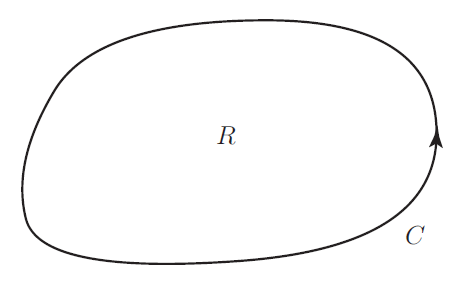
\includegraphics[width=0.6\linewidth]{fig/3.1.png}
	\caption{闭曲线$C$和它围成的区域$R$。}
\end{figure}

考虑用复坐标 $(z,\bar{z})$ 写,我们有
\begin{equation}
\begin{aligned} &d x=\frac{d z+d \bar{z}}{2},&&d y=\frac{d z-d \bar{z}}{2 i}\\ &\frac{\partial}{\partial x}=\partial+\bar{\partial}, && \frac{\partial}{\partial y}=i \partial-i \bar{\partial} 
\end{aligned}
\end{equation}
于是
\begin{equation}
	\int_{C} \frac{1}{2}(P-i Q) d z+\frac{1}{2}(P+i Q) d \bar{z}=\int_{R} d x d y(\partial(Q-i P)+\bar{\partial}(Q+i P))
\end{equation}
令
\[
T_{z z} \epsilon=Q+i P, \quad T_{\bar{z} \bar{z}} \bar{\epsilon}=Q-i P\]
得到
\begin{equation}
	\int_{R} d^{2} x\left\{\bar{\partial}\left(T_{z z} \epsilon\right)+\partial\left(T_{\bar{z} \bar{z}} \bar{\epsilon}\right)\right\}=\int_{C} \frac{T_{z z} \epsilon}{2 i} d z-\int_{C} \frac{T_{\bar{z} \bar{z}} \bar{\epsilon}}{2 i} d \bar{z}
\end{equation}
$T_{zz} $是全纯函数,$ T_{\bar{z} \bar{z}} $是反全纯函数,因此 (3.23) 改写成
\begin{equation}
\sum_{i=1}^{n}\left\langle\phi_{1} \cdots \delta \phi_{i} \cdots \phi_{n}\right\rangle+\left\langle\left(\int_{C} d z \frac{1}{i} \epsilon(z) T_{z z}-\int_{C} d \bar{z} \frac{1}{i} \bar{\epsilon}(\bar{z}) T_{\bar{z} \bar{z}}\right) \phi_{1} \cdots \phi_{n}\right\rangle=0 
\end{equation}
这里,积分路径 $C $围绕复平面上的 $z_1,\cdots,z_n $,如图3.2。
\begin{figure}[h]
	\centering
	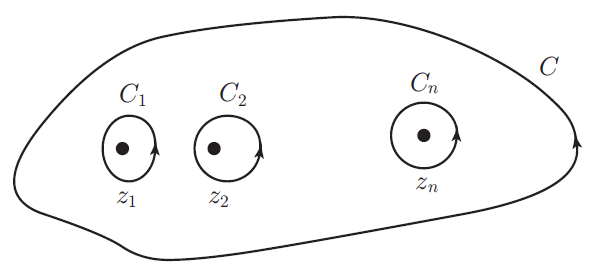
\includegraphics[width=0.6\linewidth]{fig/3.2.png}
	\caption{ 点$z_1,\cdots,z_n$,围绕它们的路径$C$,以及围绕各$z_i$的路径$C_i$。}
\end{figure}
定义 $T(z),\bar{T}(\bar{z}) $为
\[
2 \pi T_{z z}=T(z), \quad 2 \pi T_{\bar{z} \bar{z}}=\bar{T}(\bar{z})
\]
再代入初级场的无穷小变化, (3.28) 成为
\begin{equation}
\begin{aligned} &\int_{C} d z \frac{1}{2 \pi i} \epsilon(z)\left\langle T(z) \phi_{1} \cdots \phi_{n}\right\rangle-\int_{C} d \bar{z} \frac{1}{2 \pi i} \bar{\epsilon}(\bar{z})\left\langle\bar{T}(\bar{z}) \phi_{1} \cdots \phi_{n}\right\rangle\\ =&\sum_{i=1}^{n}\left(h_{i} \partial_{i} \epsilon\left(z_{i}\right)+\epsilon\left(z_{i}\right) \partial_{i}+\bar{h}_{i} \bar{\partial}_{i} \bar{\epsilon}\left(\bar{z}_{i}\right)+\bar{\epsilon}\left(\bar{z}_{i}\right) \bar{\partial}_{i}\right)\left\langle\phi_{1}\left(z_{1}, \bar{z}_{1}\right) \cdots \phi_{n}\left(z_{n}, \bar{z}_{n}\right)\right\rangle \end{aligned}
\end{equation}

这里,$ C$ 上对 $z$ 积分的被积函数,在 $C $围成的区域上是全纯的,除了插入初级场的点 $z_i$ 。根据积分路径的变形原理\footnote{[就是柯西定理]}, $C $上的积分等于围绕点 $z_i$ 的小回路 $C_i$ 上的积分之和,改写成
\[
\sum_{i=1}^{n} \int_{C_{i}} d z \frac{1}{2 \pi i} \epsilon(z)\left\langle T(z) \phi_{1} \cdots \phi_{n}\right\rangle
\]
对$ \bar{z}$ 的积分也可同样改写,那么期望值$ \langle \cdots \rangle$ 中,初级场的无穷小变化可写成
\begin{equation}
	\delta \phi_{i}\left(z_{i}, \bar{z}_{i}\right)=-\int_{C_{i}} d z \frac{1}{2 \pi i} \epsilon(z) T(z) \phi_{i}+\int_{C_{i}} d \bar{z} \frac{1}{2 \pi i} \bar{\epsilon}(\bar{z}) \bar{T}(\bar{z}) \phi_{i}
\end{equation}

因为$ C_i $可以任意小,贡献积分的只是能动张量位置 $z$ 趋于初级场位置 $z_i $时的奇异行为。具体来说,我们认为, $z\to z_i $时,期望值中可作如下展开:
\begin{equation}
T(z) \phi_{i}\left(z_{i}, \bar{z}_{i}\right)\sim\frac{h_{i}}{\left(z-z_{i}\right)^{2}} \phi_{i}\left(z_{i}, \bar{z}_{i}\right)+\frac{1}{z-z_{i}} \partial \phi_{i}\left(z_{i}, \bar{z}_{i}\right)+\text{Regular}
\end{equation}
“Regular”指展开中的常数项和$z-z_i $的正幂次项。右边在 $C_i $上积分,留数定理给出
\begin{equation}
\begin{aligned} &-\int_{C_{i}} \frac{d z}{2 \pi i} \epsilon(z)\left\{\frac{h_{i}}{\left(z-z_{i}\right)^{2}} \phi_{i}\left(z_{i}, \bar{z}_{i}\right)+\frac{1}{z-z_{i}} \partial \phi_{i}\left(z_{i}, \bar{z}_{i}\right)\right\} \\ =&-h_{i} \partial \epsilon\left(z_{i}\right) \phi_{i}\left(z_{i}, \bar{z}_{i}\right)-\epsilon\left(z_{i}\right) \partial \phi_{i}\left(z_{i}, \bar{z}_{i}\right) \end{aligned}
\end{equation}

这与初级场$ \phi(z,\bar{z}) $的无穷小变化 (3.11) 中依赖于 $\epsilon(z)$ 的项一致。依赖于 $\bar{\epsilon}(\bar{z})$ 的项也可同样得到:
\begin{equation}
\bar{T}(\bar{z}) \phi_{i}\left(z_{i}, \bar{z}_{i}\right) \sim \frac{\bar{h}_{i}}{\left(\bar{z}-\bar{z}_{i}\right)^{2}} \phi_{i}\left(z_{i}, \bar{z}_{i}\right)+\frac{1}{\bar{z}-\bar{z}_{i}} \bar{\partial} \phi_{i}\left(z_{i}, \bar{z}_{i}\right)+\text{Regular}
\end{equation}
这里的"Regular"也一样,指展开中的常数项和$ \bar{z}-\bar{z}_i $的正幂次项。

一般地,以算符之和的形式,描述算符 $A(z),B(w) $的乘积 $A(z)B(w)$ 在 $z\to w $时奇异行为的式子,称为 $A,B $的算符乘积展开(OPE)。 (3.31) 是 $T(z) $和初级场 $\phi_i(z_i,\bar{z}_i) $的OPE, $\epsilon(z)$ 代表任意无穷小共形变换。共形Ward恒等式 (3.30) ,除以 $\epsilon(z) $得到
\begin{align} 
	&\left\langle T(z) \phi_{1}\left(z_{1}, \bar{z}_{1}\right) \cdots \phi_{n}\left(z_{n}, \bar{z}_{n}\right)\right\rangle=\sum_{i=1}^{n}\left[\frac{h_{i}}{\left(z-z_{i}\right)^{2}}+\frac{1}{z-z_{i}} \partial_{i}\right]\left\langle\phi_{1}\left(z_{1}, \bar{z}_{1}\right) \cdots \phi_{n}\left(z_{n}, \bar{z}_{n}\right)\right\rangle  \\&\left\langle\bar{T}(\bar{z}) \phi_{1}\left(z_{1}, \bar{z}_{1}\right) \cdots \phi_{n}\left(z_{n}, \bar{z}_{n}\right)\right\rangle=\sum_{i=1}^{n}\left[\frac{\bar{h}_{i}}{\left(\bar{z}-\bar{z}_{i}\right)^{2}}+\frac{1}{\bar{z}-\bar{z}_{i}} \bar{\partial}_{i}\right]\left\langle\phi_{1}\left(z_{1}, \bar{z}_{1}\right) \cdots \phi_{n}\left(z_{n}, \bar{z}_{n}\right)\right\rangle
\end{align}

对全局共形变换 (3.13) ,Ward恒等式 (3.29) 的左边为零,那么初级场关联函数中加入$ T(z)$ 后,在 $z\to \infty$ 时,至少以 $z^{-4} $衰减。

\section{算符乘积和对易关系}

为更加详细地讨论局域共形对称性的Ward恒等式,我们考察二维场论中量子化与算符乘积展开的关系。

二维Euclid平面上,时间坐标是 $x^0 $,空间坐标是$ x^1$ ,引入复坐标
\begin{equation}
u=x^{0}+i x^{1}, \quad \bar{u}=x^{0}-i x^{1}
\end{equation}

令$ x^1 $有周期 $2\pi$ 。也就是说,空间是半径为 1 的圆, $(x^0,x^1) $是参数化圆柱的坐标。共形变换
\begin{equation}
	z=e^{u}, \quad \bar{z}=e^{\bar{u}}
\end{equation}

将圆柱映到复平面。无穷远过去 $x^0=-\infty$ 对应复平面原点$ z=0$ ,无穷远未来 $x^0=+\infty $对应无穷远点 $z=\infty$ 。时刻固定的圆,对应复平面上以原点为圆心的圆,时间流逝对应半径增大,如图3.3。
\begin{figure}[h]
	\centering
	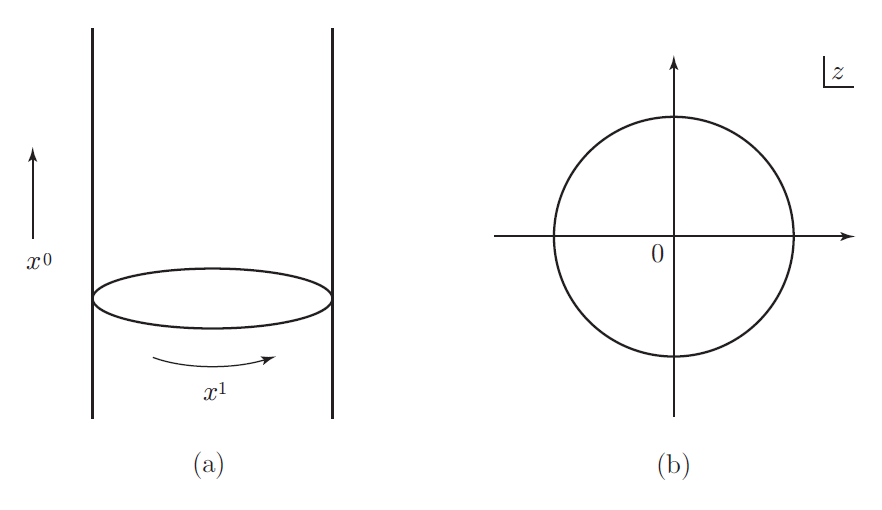
\includegraphics[width=0.6\linewidth]{fig/3.3.png}
	\caption{(a)圆柱上的坐标$(x^0,x^1)$,(b)复平面。}
\end{figure}

换句话说,时间在复平面上对应径向坐标。时间平移 $x^0\to x^0+a$ 对应复坐标 $z$ 的标度变换 $z\to e^a z$ ,空间平移 $x^1\to x^1+b$ 对应旋转 $z\to e^{ib}z $。

圆柱 $(x^0,x^1)$ 上场的期望值由编时乘积定义。在复平面上,自然就要按径向坐标排列场的顺序。这样的顺序称为\textbf{径向顺序},场的乘积称为\textbf{径向顺序积}。算符 $A(z),B(w) $的径向顺序积定义为
\begin{equation}
	R(A(z) B(w))=\left\{\begin{array}{ll} A(z) B(w), & |z|>|w| \\ B(w) A(z), & |z|<|w| \end{array}\right.
\end{equation}
复平面上共形场论中初级场的关联函数也可按径向顺序定义,接下来就展示这时得到的算符乘积与对易关系间自然的联系。

圆柱上算符$ A(x^0,x^1),B(x^0,y^1) $的等时对易关系 $[A(x^0,x^1),B(x^0,y^1)]$ ,对应复平面上的等径向坐标对易关系 $\left[A^{\prime}(z, \bar{z}), B^{\prime}(w, \bar{w})\right]$ , $|z|=|w| $。 $A'(z,\bar{z})$ 由$ A(x^0,x^1) $作共形变换 (3.37) 得到。

如果理论在特定的对称性下不变,由Noether定理,有守恒量 $J_\mu(x^0,x^1)$ ,$ \partial^\mu J_\mu=0 $。相应的守恒荷是
\begin{equation}
	Q=\int_{0}^{2 \pi} J_{0}\left(x^{0}, x^{1}\right) d x^{1}
\end{equation}
可以看到它是守恒的:
\begin{equation}
	\begin{aligned} \frac{d Q}{d x^{0}} &=\int_{0}^{2 \pi} \frac{\partial J_{0}\left(x^{0}, x^{1}\right)}{\partial x^{0}} d x^{1}=-\int_{0}^{2 \pi} \frac{\partial J_{1}\left(x^{0}, x^{1}\right)}{\partial x^{1}} d x^{1} \\ &=-J_{1}\left(x^{0}, 2 \pi\right)+J_{1}\left(x^{0}, 0\right)=0 \end{aligned}
\end{equation}
这里假定$ J_\mu(x^0,x^1)$ 满足周期性边界条件 $J_\mu(x^0,x^1+2\pi)=J_\mu(x^0,x^1) $。守恒荷生成无穷小变换,换句话说,场$ \phi$ 的无穷小变化 $\delta \phi $由对易关系给出: $\delta \phi=\epsilon[Q,\phi] $, $\epsilon $是无穷小参数。

二维无穷小共形变换对应流 $J_\mu=\epsilon^\nu T_{\mu\nu}$ ,守恒荷用复坐标 $(z,\bar{z}) $表达为
\begin{equation}
	Q=\int_{C_{0}} \frac{d z}{2 \pi i} \epsilon(z) T(z)+\int_{C_{0}} \frac{d \bar{z}}{2 \pi i} \bar{\epsilon}(\bar{z}) \bar{T}(\bar{z})
\end{equation}
这里, $C_0$ 是围绕原点的闭合曲线。

计算守恒荷与场的对易关系时,会出现同一点处场的乘积。因为这是发散的,需要先正规化计算出有限的量,再恢复正规化的参数。定义等时对易关系时,让时间发生微小的变化 $\epsilon $( $\epsilon $是正数)以正规化:
\[
\left[A\left(x^{0}, x^{1}\right), B\left(x^{0}, y^{1}\right)\right]= \lim _{\epsilon \rightarrow 0}\left(A\left(x^{0}+\epsilon, x^{1}\right) B\left(x^{0}, y^{1}\right)-B\left(x^{0}, y^{1}\right) A\left(x^{0}-\epsilon, x^{1}\right)\right)
\]
在复平面上,这样的操作对应
\begin{equation}
[A(z, \bar{z}), B(w, \bar{w})]=\lim _{|z| \rightarrow|w| \atop|z|>|w|} A(z, \bar{z}) B(w, \bar{w})-\lim _{|z| \rightarrow|w| \atop|w|>|z|} B(w, \bar{w}) A(z, \bar{z})
\end{equation}
换句话说,算符乘积被定义为总按径向顺序。

无穷小共形变换的生成元$ Q $与初级场 $\phi(w,\bar{w})$ 的对易关系,用径向顺序积写成
\begin{equation}
	\begin{aligned} \left[Q, \phi(w, \bar{w})\right]&=\int_{C_{1}} \frac{d z}{2 \pi i} \epsilon(z) T(z) \phi(w, \bar{w})-\int_{C_{2}} \frac{d z}{2 \pi i} \phi(w, \bar{w}) \epsilon(z) T(z)+\text{含}\bar{T}\text{的项}\\ &=\left(\int_{C_{1}} \frac{d z}{2 \pi i}-\int_{C_{2}} \frac{d z}{2 \pi i}\right) R(\epsilon(z) T(z) \phi(w, \bar{w}))+\text{含}\bar{T}\text{的项}\end{aligned}
\end{equation}
这里, $C_1 $是满足$ |z|>|w| $的围绕原点的闭合曲线, $C_2$ 则是满足 $|z|<|w| $。这两个积分的差,可转换成围绕 $z=w $的圆$ C_w$ 上的积分,如图3.4:
\begin{equation}
	[Q, \phi(w, \bar{w})]=\int_{C_{w}} \frac{d z}{2 \pi i} R(\epsilon(z) T(z) \phi(w, \bar{w}))+\text{含}\bar{T}\text{的项}
\end{equation}

\begin{figure}[h]
	\centering
	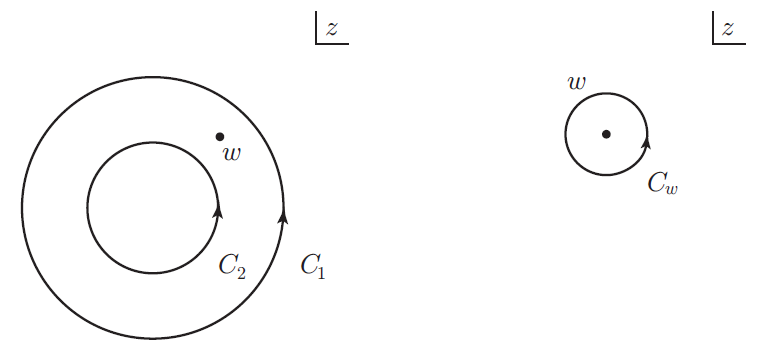
\includegraphics[width=0.6\linewidth]{fig/3.4}
	\caption{$C_1$:满足$|z| >|w|$的闭合曲线,$C_2$:满足$|z|<|w|$的闭合曲线,$C_w$:$C_1-C_2$变形得到的围绕$w$的闭合曲线。}
\end{figure}

因为$ C_w $可以任意小,贡献积分的是 $z\to w $,$T(z)$ 与$ \phi(w,\bar{w})$ 的OPE。代入OPE
\[
	T(z) \phi(w, \bar{w})=\frac{h}{(z-w)^{2}} \phi(w, \bar{w})+\frac{1}{z-w} \partial \phi(w, \bar{w})+\text{Regular}
\]
我们有
\begin{equation}
	\begin{aligned} \left[Q, \phi(w, \bar{w})\right]&=\int_{C_{w}} \frac{d z}{2 \pi i} \epsilon(z)\left\{\frac{h}{(z-w)^{2}} \phi_{i}(w, \bar{w})+\frac{1}{z-w} \partial \phi_{i}(w, \bar{w})\right\}+\text{含}\bar{T}\text{的项}\\ &=h \partial \epsilon(w) \phi(w, \bar{w})+\epsilon(w) \partial \phi(w, \bar{w})+\bar{h} \bar{\partial} \bar{\epsilon}(\bar{w}) \phi(w, \bar{w})+\bar{\epsilon}(\bar{w}) \bar{\partial} \phi(w, \bar{w}) \end{aligned}
\end{equation}
于是,通过$ {\color{red}-}\delta\phi=[Q,\phi] $得到了 $\phi$ 的无穷小变化\footnote{[按照本书的符号约定,似乎这里漏掉了一个负号,下一节也存在同样的问题,均使用红色标出]}。用径向顺序积定义的对易关系可由OPE计算。
\section{Virasoro代数}
\subsection{中心荷}
考虑能动张量 $T(z),\bar{T}(\bar{z})$ 的关联函数。因为能动张量 $T(z) $本来就是 $(2,0) $型张量,我们预期它是共形权为 $(2,0) $的初级场。同样, $\bar{T}(\bar{z})$ 是 $(0,2) $型张量,我们预期它是共形权为 $(0,2) $的初级场。$ T(z)$ 的单点函数 $\langle T(z)\rangle $平移不变,因此是不依赖于$ z$的常数,设为零:
\begin{equation}
	\langle T(z)\rangle=0, \quad\langle\bar{T}(\bar{z})\rangle=0
\end{equation}
全局共形不变性将$ T(z)$ 的两点函数限制成
\begin{equation}
	\langle T(z) T(w)\rangle=\frac{\frac{c}{2}}{(z-w)^{4}}, \quad\langle\bar{T}(\bar{z}) \bar{T}(\bar{w})\rangle=\frac{\frac{\bar{c}}{2}}{(\bar{z}-\bar{w})^{4}}
\end{equation}
这里, $c,\bar{c} $是常数。两点函数的形式 (3.47) 说明,$ T(z) $和$ T(w) $的OPE有 $z-w $的四阶极点,再由 $T(w) $本来就是$ (2,0)$ 型张量,得到OPE的形式是
\begin{equation}
	T(z) T(w)=\frac{\frac{c}{2}}{(z-w)^{4}}+\frac{2 T(w)}{(z-w)^{2}}+\frac{\partial T(w)}{z-w}+\cdots
\end{equation}

这里,$\cdots$代表展开中$ z-w $的非负幂次项。同样,$ \bar{T}(\bar{z})$ 和 $\bar{T}(\bar{w})$ 的OPE是
\begin{equation}
	\bar{T}(\bar{z}) \bar{T}(\bar{w})=\frac{\frac{\bar{c}}{2}}{(\bar{z}-\bar{w})^{4}}+\frac{2 \bar{T}(\bar{w})}{(\bar{z}-\bar{w})^{2}}+\frac{\partial \bar{T}(\bar{w})}{\bar{z}-\bar{w}}+\cdots
\end{equation}
常数 $c,\bar{c} $称为\textbf{中心荷}。

能动张量 $T(z) $的无穷小共形变化是
\begin{equation}
	{\color{red}-}\delta T(w)=\int \frac{d z}{2 \pi i} \epsilon(z) T(z) T(w)
\end{equation}
右边代入OPE (3.48) ,得到\footnote{$n$阶极点留数可以使用下式计算:\[\Res[f(z),a]=\lim_{z\to a}\frac{1}{(n-1)!}\frac{d^{n-1}}{dz^{n-1}}\left[(z-a)^nf(z)\right]\]}
\begin{equation}
	\begin{aligned} {\color{red}-}\delta T(w) &=\int \frac{d z}{2 \pi i} \epsilon(z)\left\{\frac{\frac{c}{2}}{(z-w)^{4}}+\frac{2 T(w)}{(z-w)^{2}}+\frac{\partial T(w)}{z-w}\right\} \\ &=\frac{c}{2} \frac{1}{3 !} \partial^{3} \epsilon(w)+2 \partial \epsilon(w) T(w)+\epsilon(w) \partial T(w) \end{aligned}
\end{equation}

能动张量 $T(w)$ 的无穷小共形变化,与初级场的不同只在于多了含$ \epsilon(w) $三阶导的项。在全局共形变换的情形, $\epsilon(w) $是$ w$ 的二次多项式,这项就为零。因此,全局共形变换下,$ T(w) $的行为同初级场一样,那么它是准初级场(见2.3节)。

有限共形变换 $z \rightarrow w=w(z) $下, $T(z) $变换为:\footnote{[此式对于一般的共形变换证明是较难的,但是对于无穷小变换可以很快地验证,本章末尾会对自由费米子和玻色子进行简要证明]}
\begin{equation}
	T(z) \rightarrow T^{\prime}(w)=T(z)\left(\frac{d w}{d z}\right)^{-2}-\frac{c}{12} S(w, z)\left(\frac{d w}{d z}\right)^{-2}
\end{equation}
$S(w,z)$ 是\textbf{Schwarz导数},定义为
\begin{equation}
	S(w, z)=\frac{\partial_{z} w \partial_{z}^{3} w-\frac{3}{2}\left(\partial_{z}^{2} w\right)^{2}}{\left(\partial_{z} w\right)^{2}}
\end{equation}

对全局 $SL(2,\mathbb{C})$ 变换$ w=(az+b)/(cz+d) $,有 $S(w,z)=0 $。同时,对共形变换 $f=f(z),w=w(f)$ 的复合 $w(f(z)) $,有
\begin{equation}
	S(w, z)=\left(\partial_{z} f\right)^{2} S(w, f)+S(f, z)
\end{equation}
中心荷出现在能动张量的两点函数中,导致能动张量的变换规则不同于常规的 $(2,0) $型张量。量子效应破坏守恒律和变换规则的现象,称为\textbf{反常}。 $c$ 就是表现\textbf{共形反常}的指标。

\subsection{ Virasoro代数}

将无穷小共形变换Laurent展开成:$\epsilon(z)=\sum_{n=-\infty}^{\infty} \epsilon_{n} z^{n+1}, \bar{\epsilon}(\bar{z})=\sum_{n=-\infty}^{\infty} \bar{\epsilon}_{n} \bar{z}^{n+1}\ (n\in \mathbb{Z}) $, $\epsilon_n,\bar{\epsilon}_n $对应的荷记作 $\epsilon_nL_n,\bar{\epsilon}_n\bar{L}_n $,那么$ L_n,\bar{L}_n\ (n\in \mathbb{Z})$ 是
\begin{equation}
	L_{n}=\oint \frac{d z}{2 \pi i} z^{n+1} T(z), \quad \bar{L}_{n}=\oint \frac{d \bar{z}}{2 \pi i} \bar{z}^{n+1} \bar{T}(\bar{z})
\end{equation}
这相当于 $T(z),\bar{T}(\bar{z}) $的Laurent展开
\begin{equation}
	T(z)=\sum_{n=-\infty}^{\infty} L_{n} z^{-n-2}, \quad \bar{T}(\bar{z})=\sum_{n=-\infty}^{\infty} \bar{L}_{n} \bar{z}^{-n-2}
\end{equation}
共形变换的荷可写成
\begin{equation}
	Q=\sum_{n=-\infty}^{\infty} \epsilon_{n} L_{n}+\bar{\epsilon}_{n} \bar{L}_{n}
\end{equation}

我们来计算$ L_n 和 L_m $( $n,m\in \mathbb{Z}$ )的对易子 $[L_n,L_m] $。先计算 $L_n $和 $T(w)$ 的对易关系,再围绕原点作积分 $\oint \frac{d w}{2 \pi i} w^{m+1}$ ,也就是
\begin{equation}
	\left[L_{n}, L_{m}\right]=\oint \frac{d w}{2 \pi i} w^{m+1} \int_{C_{w}} \frac{d z}{2 \pi i} z^{n+1} T(z) T(w)
\end{equation}
$C_w$ 是围绕$ z=w $的闭合曲线。右边代入OPE (3.48) :
\[
	\oint \frac{d w}{2 \pi i} w^{m+1} \int_{C_{w}} \frac{d z}{2 \pi i} z^{n+1}\left\{\frac{\frac{c}{2}}{(z-w)^{4}}+\frac{2 T(w)}{(z-w)^{2}}+\frac{\partial T(w)}{z-w}\right\}
\]
用留数定理计算对 $z$ 的积分,再根据$ L_n$ 的定义改写:
\begin{equation}
	\begin{aligned} &\oint \frac{d w}{2 \pi i} w^{m+1}\left\{\frac{c}{2} \frac{(n+1) n(n-1)}{3 !} w^{n-2}+2(n+1) T(w) w^{n}+\partial T(w) w^{n+1}\right\} \\ =&\frac{c}{12}(n+1) n(n-1) \delta_{n+m, 0}+2(n+1) L_{n+m}-(n+m+2) L_{n+m} \end{aligned}
\end{equation}
最后一项是这样算的:
\[
\oint \frac{d w}{2 \pi i} w^{m+n+2} \partial T(w)=\oint \frac{d w}{2 \pi i} \left[\partial\left(w^{m+n+2} T(w)\right)-(m+n+2) w^{m+n+1} T(w)\right]
\]
全导数不贡献积分。于是, $L_n,L_m$ 的对易关系是
\begin{equation}
	\left[L_{n}, L_{m}\right]=(n-m) L_{n+m}+\frac{c}{12} n\left(n^{2}-1\right) \delta_{n+m, 0}
\end{equation}

这个代数称为\textbf{Virasoro代数},$ L_n$ 是Virasoro代数的生成元。中心荷 $c$ 是常规的数,与Virasoro代数的生成元对易,这样的元素称为中心。因为右边也可看成$ L_n $和 $c$ 的线性组合,我们称这个代数是第1章讨论的二维共形代数加上$ c$ \textbf{扩张}得到的,是它的\textbf{中心扩张}。

$\bar{L}_n$ 也是同一代数的生成元:
\begin{equation}	
\left[\bar{L}_{n}, \bar{L}_{m}\right]=(n-m) \bar{L}_{n+m}+\frac{\bar{c}}{12} n\left(n^{2}-1\right) \delta_{n+m, 0}
\end{equation}
$T(z) $和 $\bar{T}(\bar{w}) $没有OPE,因此
\begin{equation}
\left[L_{n}, \bar{L}_{m}\right]=0	
\end{equation}
$L_{\pm 1},L_0 $生成全局共形变换,相应的代数中不出现 $c $,具体来说是
\begin{equation}
\left[L_{0}, L_{\pm 1}\right]=\mp L_{\pm 1}, \quad\left[L_{1}, L_{-1}\right]=2 L_{0}
\end{equation}
这个代数是 $\mathfrak{sl}(2,\mathbb{C})$ 。

\subsection{CFT的Hilbert空间}
我们来考察共形场论的Hilbert空间与Virasoro代数的表示间的关系。将初级场的关联函数表示成场算符乘积的真空期望值:
\begin{equation}
	\left\langle\phi_{1}\left(z_{1}, \bar{z}_{1}\right) \cdots \phi_{N}\left(z_{N}, \bar{z}_{N}\right)\right\rangle=\left\langle 0\left|R\left(\phi_{1}\left(z_{1}, \bar{z}_{1}\right) \cdots \phi_{N}\left(z_{N}, \bar{z}_{N}\right)\right)\right| 0\right\rangle
\end{equation}
$|0\rangle$ 是对应真空的右矢。关联函数在全局共形变换下不变。无穷小Ward恒等式是
\begin{equation}
	\begin{aligned} 0 &=\sum_{j=1}^{N}\left\langle\phi_{1}\left(z_{1}, \bar{z}_{1}\right) \cdots \delta \phi_{j}\left(z_{j}, \bar{z}_{j}\right) \cdots \phi_{N}\left(z_{N}, \bar{z}_{N}\right)\right\rangle \\ &=\sum_{j=1}^{N}\left\langle 0\left|R\left(\phi_{1}\left(z_{1}, \bar{z}_{1}\right) \cdots\left[Q, \phi_{j}\left(z_{j}, \bar{z}_{j}\right)\right] \cdots \phi_{N}\left(z_{N}, \bar{z}_{N}\right)\right)\right| 0\right\rangle \end{aligned}
\end{equation}
这里, $Q=\epsilon_{-1} L_{-1}+\epsilon_{0} L_{0}+\epsilon_{1} L_{1}$ 。右边也可写成
\[
	\left\langle 0\left|\left[Q, \phi_{1}\left(z_{1}, \bar{z}_{1}\right) \cdots \phi_{N}\left(z_{N}, \bar{z}_{N}\right)\right]\right| 0\right\rangle
\]
这要对任意 $\epsilon_{\pm1},\epsilon_0$ 成立,真空右矢 $|0\rangle $和左矢 $\langle 0|$ 就要在$ m=0,\pm 1$ 时满足
\begin{equation}
	L_{m}|0\rangle=0, \quad\langle 0| L_{m}=0
\end{equation}
这意味着真空是 $SL(2,\mathbb{C}) $不变的。

Virasoro代数的一般生成元$ L_m $作用在 $|0\rangle $上需要满足的条件,由 $T(z)|0\rangle $在 $z\to 0 $时正规来确定。根据 $T(z)$ 的Laurent展开式
\begin{equation}
	T(z)|0\rangle=\sum_{n=-\infty}^{\infty} L_{n}|0\rangle z^{-n-2}
\end{equation}
可以知道, $z\to 0$ 时不出现奇异性要求
\begin{equation}
	L_{n}|0\rangle=0, \quad n \geq-1
\end{equation}
对真空左矢$ \langle 0| $,则是 $\langle 0|T(z)$ 在 $z\to \infty $时正规,这要求\footnote{要看到这点,在$z \to \infty$处改用坐标$w = 1/z$。能动张量的变换规则给出$T(z) = \left( \frac{\partial w}{\partial z} \right)^2 T'(w)=w^4 T'(w)$。于是我们要求$\langle 0 | T'(w) = \langle 0 | z^4 T(z)$在$z \to \infty$时正规。}
\begin{equation}
	0=\langle 0| L_{n}, \quad n \leq 1
\end{equation}
用这个性质可以计算$ T(z) $的两点函数$ \langle T(z)T(w)\rangle $。$ |z|>|w|$ 时,由 (3.68),(3.69) 有
\begin{equation*}
	\begin{aligned} \langle 0|T(z) T(w)| 0\rangle &=\sum_{n=-\infty}^{\infty} \sum_{m=-\infty}^{\infty} z^{-n-2} w^{-m-2}\left\langle 0\left|L_{n} L_{m}\right| 0\right\rangle \\ &=\sum_{n=0}^{\infty} \sum_{m=-\infty}^{-2} z^{-n-2} w^{-m-2}\left\langle 0\left|L_{n} L_{m}\right| 0\right\rangle \end{aligned}
\end{equation*}
右边代入Virasoro代数 (3.60) 得到
\begin{equation*}
\begin{aligned} & \sum_{n=0}^{\infty} \sum_{m=-\infty}^{-2} z^{-n-2} w^{-m-2}\left\langle 0\left|\left(L_{m} L_{n}+\left[L_{n}, L_{m}\right]\right)\right| 0\right\rangle \\ =& \sum_{n=0}^{\infty} \sum_{m=-\infty}^{-2} z^{-n-2} w^{-m-2}\left\langle 0\left|\left\{(n-m) L_{n+m}+\frac{c}{12} n\left(n^{2}-1\right) \delta_{n+m, 0}\right\}\right| 0\right\rangle \\ =& \sum_{n=0}^{\infty} \frac{c}{12} n\left(n^{2}-1\right) \frac{1}{z^{2} w^{2}}\left(\frac{w}{z}\right)^{n} \\ =& \frac{\frac{c}{2}}{(z-w)^{4}} \end{aligned}
\end{equation*}
这复现了OPE的结果。

\subsection{BPZ共轭}
CFT的Hilbert空间上定义有自然的Hermite共轭(BPZ共轭)。它是将二维Minkowski时空中的Hermite共轭推广到Euclid空间得到的。

首先,定义作用在Hilbert空间上的算符的共轭。考虑Minkowski时空 $(t,x) $中的场 $A(t,x) $。时间演化由Hamiltonian生成, $t $时刻的场与 $t=0 $时的关系是
$$
A(t, x)=e^{i H t} A(0, x) e^{-i H t}
$$
这个关系式的Hermite共轭是
$$
A(t, x)^{\dagger}=e^{i H t} A(0, x)^{\dagger} e^{-i H t}
$$
也就是说,时间演化后作Hermite共轭,等价于 $t=0$ 时取Hermite共轭再时间演化。

时间 $t$ 解析延拓( $\tau=+i t$ )到虚轴\footnote{[原书为$\tau=-i t$]},就得到Euclid空间 $(\tau,x)$ 中的时间演化:
$$
A(\tau, x)=e^{H \tau} A(0, x) e^{-H \tau}
$$
这个关系式的Hermite共轭是
$$
A(\tau, x)^{\dagger}=e^{-H \tau} A(0, x)^{\dagger} e^{H \tau}
$$
也就是说,时间演化后作Hermite共轭,不同于 $\tau=0 $时取Hermite共轭再时间演化,还需要加上时间反演 $\tau \to -\tau$ 。我们将这个复合变换定义为Euclid空间中的“Hermite”共轭,本节用$ {}^+ $表示:
$$
A(\tau, x)^{+}=e^{H \tau} A(0, x)^{+} e^{-H \tau}
$$
在圆柱 $(x^0,x^1) $上定义共形权是 $(h,\bar{h}) $的初级场 $\phi'(u,\bar{u})$ ,它的“Hermite”共轭是
$$
\phi^{\prime}(u, \bar{u})^{+}=\phi^{\prime}(-\bar{u},-u)
$$
这里,$ u=x^{0}+i x^{1}, \bar{u}=x^{0}-i x^{1} $。通过共形变换 $z=e^{u}, \bar{z}=e^{\bar{u}} $,将$ \phi'(u,\bar{u})$ 映到复平面上,得到的初级场记作 $\phi(z,\bar{z}) $,它与$ \phi'(u,\bar{u})$ 的关系是
$$
\phi(z, \bar{z})=\left(\frac{d z}{d u}\right)^{-h}\left(\frac{d \bar{z}}{d \bar{u}}\right)^{-\bar{h}} \phi^{\prime}(u, \bar{u})
$$
由 $dz/du=z,d\bar{z}/d\bar{u}=\bar{z} $得到
\begin{equation}
	\phi(z, \bar{z})=z^{-h} \bar{z}^{-\bar{h}} \phi^{\prime}(u, \bar{u})
\end{equation}
那么 $\phi(z,\bar{z}) $的“Hermite”共轭是
$$
\phi(z, \bar{z})^{+}=\bar{z}^{-h} z^{-\bar{h}} \phi^{\prime}(u, \bar{u})^{+}
$$
另一方面, $(u,\bar{u}) $时间反演成$ (-\bar{u},-u)$ 后,$ (z,\bar{z}) $就会变成 $(1/\bar{z},1/z)$ ,因此 (3.70) 时间反演后成为
$$
\phi\left(\frac{1}{\bar{z}}, \frac{1}{z}\right)=\left(\frac{1}{\bar{z}}\right)^{-h}\left(\frac{1}{z}\right)^{-\bar{h}} \phi^{\prime}(-\bar{u}, -u)
$$
于是有
\begin{equation}
	\phi(z, \bar{z})^{+}=\bar{z}^{-2 h} z^{-2 \bar{h}} \phi\left(\frac{1}{\bar{z}}, \frac{1}{z}\right)
\end{equation}
同时,初级场 $\phi(z,\bar{z}) $在 $w=1/z $变换下成为
\begin{equation}
\begin{aligned} \tilde{\phi}(w, \bar{w}) &=\left(\frac{d w}{d z}\right)^{-h}\left(\frac{d \bar{w}}{d \bar{z}}\right)^{-\bar{h}} \phi(z, \bar{z}) \\ &=\left(-w^{2}\right)^{-h}\left(-\bar{w}^{2}\right)^{-\bar{h}} \phi\left(\frac{1}{w}, \frac{1}{\bar{w}}\right) \end{aligned}
\end{equation}
与 (3.71) 比对得到
\begin{equation}
	\phi(z, \bar{z})^{+}=(-1)^{h+\bar{h}} \tilde{\phi}(\bar{z}, z)
\end{equation}
因为能动张量 $T(z)$ 的共形权是 $(2,0) $, (3.71) 给出
\begin{equation}
	T(z)^{+}=T\left(\frac{1}{\bar{z}}\right) \frac{1}{\bar{z}^{4}}
\end{equation}
代入 $T(z)$ 的Laurent展开 (3.56) ,得到
$$
\sum_{m=-\infty}^{\infty} L_{m}^{+} \bar{z}^{-m-2}=\bar{z}^{-4} \sum_{n=-\infty}^{\infty} L_{n} \bar{z}^{n+2}
$$
从而
\begin{equation}
	L_n^+=L_{-n}
\end{equation}

CFT Hilbert空间中态矢 $|\phi\rangle$的BPZ共轭按如下方式定义:首先, $SL(2,\mathbb{C}) $不变真空$ |0\rangle$ 的BPZ共轭是$ \langle 0|$ :
$$
(|0\rangle)^{+}=\langle 0|
$$
初级场 $\phi(z,\bar{z}) $对应的态矢 $|\phi\rangle$ 定义为
\begin{equation}
	|\phi\rangle=\lim _{z, \bar{z} \rightarrow 0} \phi(z, \bar{z})|0\rangle
\end{equation}
$z=\bar{z}=0 $对应无穷远过去 $x^0\to -\infty$ 。态 $|\phi\rangle$ 的BPZ共轭,定义为无穷远未来 $z\to\infty $( $x^0\to +\infty $)时的态
\begin{equation}
	\langle\phi|=\lim _{w, \bar{w} \rightarrow 0}\langle 0| \tilde{\phi}(w, \bar{w})(-1)^{h+\bar{h}}=\lim _{z, \bar{z} \rightarrow \infty}\langle 0| \phi(z, \bar{z}) z^{2 h} \bar{z}^{2 \bar{h}}
\end{equation}
$z\to \infty$ 就对应$ w\to 0$ 。根据 (3.73) , $\langle \phi| $正是 $|\phi\rangle $的“Hermite”共轭 $(|\phi\rangle)^+ $。之后将讨论,CFT的Hilbert空间一般通过负模Virasoro代数生成元$ L_{-n} $( $n=1,2,\ldots$)作用在初级场对应的态矢上来构造。根据 (3.75) ,态矢$ L_{-n_{1}} \cdots L_{-n_{N}}|\phi\rangle$ 的“Hermite”共轭是 $\langle\phi| L_{n_{N}} \cdots L_{n_{1}} $。

因此,在CFT中,态矢一般可通过算符作用在$ SL(2,\mathbb{C}) $不变真空上来构造,且算符对应着态矢。(恒等算符 $\boldsymbol{I} $对应真空)这称为\textbf{态-算符对应}。

接下来解释CFT的一些简单例子,自由玻色子和自由费米子。
\section{自由标量场}
用复坐标 $(z,\bar{z})$ 写,无相互作用标量场(自由玻色子) $\varphi(z,\bar{z}) $的作用量是
\begin{equation}
	S=\frac{1}{8 \pi} \int d^{2} x \partial^{\mu} \varphi \partial_{\mu} \varphi=\frac{1}{2 \pi} \int d^{2} x \partial_{z} \varphi \partial_{\bar{z}} \varphi
\end{equation}
这是 (2.52) 中令 $\varphi \to \varphi/\sqrt{4\pi}$ 得到的。 $\varphi$ 的两点函数是
\begin{equation}
	\langle\varphi(z, \bar{z}) \varphi(w, \bar{w})\rangle=-\ln |z-w|^{2}
\end{equation}
这里, $-\ln |z-w|^{2}$ 是Laplacian $\partial_z\partial_{\bar{z}} $的Green函数,这等价于二维中点电荷产生的势。这个意义上,自由玻色子系统也称为Coulomb气体。

由运动方程$ \partial_{z} \partial_{\bar{z}} \varphi=0 $, $\varphi(z,\bar{z})$ 可分成正反全纯部分:
\begin{equation}
	\varphi(z, \bar{z})=\varphi(z)+\bar{\varphi}(\bar{z})
\end{equation}
那么$ \varphi(z) $和 $\bar{\varphi}(\bar{z}) $的两点函数是
\begin{align} &\langle\varphi(z) \varphi(w)\rangle=-\ln (z-w) \\ &\langle\bar{\varphi}(\bar{z}) \bar{\varphi}(\bar{w})\rangle=-\ln (\bar{z}-\bar{w}) \end{align}
共形变换 $z\to w=f(z)$ 下,标量场变换为\footnote{二维下标量场的共形维数是 $\Delta=(D-2)/2=0 $,见2.1节}
\[\varphi(z, \bar{z})=\varphi^{\prime}(w, \bar{w})
\]
对无穷小变换 $w=z-\epsilon(z) $,标量场在同一点上的无穷小变化是
$$
\delta \varphi(z, \bar{z})=\epsilon(z) \partial \varphi+\bar{\epsilon}(\bar{z}) \bar{\partial} \bar{\varphi}(\bar{z})
$$
关于$ z $求导得到
\begin{equation}
	\delta \partial \varphi(z)=\partial \epsilon \partial \varphi+\epsilon \partial^{2} \varphi
\end{equation}
这个无穷小变换的生成元是能动张量 $T(z),\bar{T}(\bar{z}) $,无穷小变化 (3.83) 用OPE表示是
\begin{equation}
	T(z) \partial \varphi(w)=\frac{\partial \varphi(w)}{(z-w)^{2}}+\frac{\partial^{2} \varphi(w)}{z-w}+\cdots
\end{equation}
因此$ \partial \varphi(z) $是共形权为 $(1,0) $的初级场。

另一方面, $T(z),\bar{T}(\bar{z})$ 用 $\partial \varphi(z),\bar{\partial}\bar{\varphi}(\bar{z}) $表示是
\begin{equation}
	T(z)=-\frac{1}{2}:(\partial \varphi)^{2}:(z), \quad \bar{T}(\bar{z})=-\frac{1}{2}:(\bar{\partial} \bar{\varphi})^{2}:(\bar{z})
\end{equation}
这里,记号
$$
:AB:(z)\quad\text{或}\quad(AB)(z)
$$
表示算符$ A(z),B(z)$ 的\textbf{正规顺序积}。也就是取算符乘积 $A(w)B(z) $在两点接近即 $w\to z $时的极限,再减去发散项得到的算符。

简单起见,之后只考虑全纯部分。由 (3.81) , $\partial \varphi(z) $的两点函数是
\begin{equation}
	\langle\partial \varphi(z) \partial \varphi(w)\rangle=-\partial_{z} \partial_{w} \ln (z-w)=-\frac{1}{(z-w)^{2}}
\end{equation}
$\partial \varphi(z) $间的OPE是
\begin{equation}
	\partial \varphi(z) \partial \varphi(w)=-\frac{1}{(z-w)^{2}}+\cdots
\end{equation}
那么正规顺序积 $:(\partial \varphi)^2:$ 就通过OPE (3.87) 中减去奇异项来定义:
\begin{equation}
:(\partial \varphi)^{2}:(w)=\lim _{z \rightarrow w}\left(\partial \varphi(z) \partial \varphi(w)+\frac{1}{(z-w)^{2}}\right)
\end{equation}

为从 $\partial \varphi(z) $间的OPE,来计算 $T(z)$ 和 $\partial \varphi(w)$ 的OPE,以及 $T(z) $间的OPE,接下来总结一下如何计算正规顺序积给出的复合算符间的OPE。

\section{复合算符间的OPE}
令 $A(z),B(z),C(z)$ 是共形权为整数(这样有玻色对易关系\footnote{因为共形权的差是自旋,见3.1节})的共形场。 $A(z) 和 B(w) $的OPE表示成
\begin{equation}
	A(z) B(w)=\sum_{n=-\infty}^{N} \frac{\{A B\}_{n}(w)}{(z-w)^{n}}
\end{equation}
OPE中的奇异部分记作
\begin{equation}
	\wick{\c A(z) \c B}(w)=\sum_{n=1}^{N} \frac{\{A B\}_{n}(w)}{(z-w)^{n}}
\end{equation}
这里, $\{AB\}_0(w)$ 就是 $A$ 和$ B$ 的正规顺序积$ (AB)(w) $:
\begin{equation}
	\begin{aligned} \{A B\}_{0}(w) &=(A B)(w) \\ &=\lim _{z \rightarrow w}\left(A(z) B(w)-	\wick{\c A(z) \c B}(w)\right) \end{aligned}
\end{equation}
$(AB)(w) $也是OPE中 $(z-w)^0$那项的系数:
\begin{equation}
	(A B)(w)=\frac{1}{2 \pi i} \oint d z \frac{A(z) B(w)}{z-w}
\end{equation}

一般来说,$ (AB)(w) $不同于 $(BA)(w)$ 。事实上,由OPE
\begin{equation}
	B(z) A(w)=A(w) B(z)=\sum_{n=-\infty}^{N} \frac{\{A B\}_{n}(z)}{(w-z)^{n}}
\end{equation}
可以得到
\begin{equation}
	(B A)(w)=\sum_{n=0}^{N}(-1)^{n} \frac{1}{n !} \partial^{n}\{A B\}_{n}(w)
\end{equation}
根据Wick定理,对算符 $A(z),B(z),C(z) $, $A(z) $和 $(BC)(w) $的OPE是\footnote{F. A. Bais, P. Bouwknegt, M. Surridge and K. Schoutens, Nucl. Phys. B 304 (1988) 348.}
\begin{equation}
	A(z)(B C)(w)=\frac{1}{2 \pi i} \oint \frac{d x}{x-w}\left\{ \wick{\c A(z) \c B}(x) C(w)+B(x) \wick{\c A(z) \c C}(w)\right\}
\end{equation}
例如,要计算$ \partial \varphi(z) $和 $(\partial \varphi \partial \varphi)(w)$ 的OPE,用 (3.95) 就转换成计算 $w $处的留数:
\begin{equation}
	\begin{aligned} \partial \varphi(z)(\partial \varphi \partial \varphi)(w)=& \frac{1}{2 \pi i} \oint \frac{d x}{x-w}\left\{-\frac{1}{(z-x)^{2}} \partial \varphi(w)+\partial \varphi(x)\left(\frac{-1}{(z-w)^{2}}\right)\right\} \\ =&-\frac{\partial \varphi(w)}{(z-w)^{2}}-\frac{\partial \varphi(w)}{(z-w)^{2}} \\ =& \frac{-2 \partial \varphi(w)}{(z-w)^{2}} \end{aligned}
\end{equation}
因此,$ T(z)$ 和 $\partial\varphi(w) $的OPE是
\begin{equation}
	\begin{aligned} T(z) \partial \varphi(w) &=\partial \varphi(w) T(z)=\frac{\partial \varphi(z)}{(w-z)^{2}} \\ &=\frac{\partial \varphi(w)}{(z-w)^{2}}+\frac{\partial^{2} \varphi(w)}{z-w} \end{aligned}
\end{equation}
可以看到, $\partial \varphi(z) $是共形权 $h=1 $的初级场。

接下来计算 $T(z) $和 $T(w) $的OPE。先用 (3.95) 得到
\begin{equation}
	\begin{aligned} T(z) T(w) &=-\frac{1}{2} T(z)(\partial \varphi \partial \varphi)(w) \\ &=-\frac{1}{2} \frac{1}{2 \pi i} \oint \frac{d x}{x-w}\left\{\wick{\c T(z) \partial \c \varphi}(x) \partial \varphi(w)+\partial \varphi(x) \wick{\c T(z) \partial\c \varphi}(w)\right\} \end{aligned}
\end{equation}
再用 $T(z)$ 和 $\partial \varphi(x)$ 的OPE,可以看到右边第一项中除了有这个OPE的贡献,还有$ \partial \varphi(z) $间OPE的贡献,这提高了奇异的程度:
\begin{equation}
	\begin{aligned} &- \frac{1}{2} \frac{1}{2 \pi i} \oint \frac{d x}{x-w}\left\{\frac{\partial \varphi(x)}{(z-x)^{2}}+\frac{\partial^{2} \varphi(x)}{z-x}\right\} \partial \varphi(w) \\ =&-\frac{1}{2} \frac{1}{2 \pi i} \oint \frac{d x}{x-w}\left\{\frac{1}{(z-x)^{2}}\left(\frac{-1}{(x-w)^{2}}+\left(\partial \varphi \partial \varphi\right)(w)\right)\right.\\ &\left.+\frac{1}{z-x}\left(\frac{2}{(x-w)^{3}}+(\partial^2 \varphi \partial \varphi)(w)\right)\right\} \end{aligned}
\end{equation}
由Cauchy-Goursat公式有
\begin{align} &\frac{1}{2 \pi i} \oint \frac{d x}{(x-w)^{3}} \frac{1}{(z-x)^{2}}=\left.\frac{1}{2 !} \frac{d^{2}}{d x^{2}} \frac{1}{(z-x)^{2}}\right|_{x=w}=\frac{3}{(z-w)^{4}} \\ &\frac{1}{2 \pi i} \oint \frac{d x}{(x-w)^{4}} \frac{1}{z-x}=\left.\frac{1}{3 !} \frac{d^{3}}{d x^{3}} \frac{1}{z-x}\right|_{x=w}=\frac{1}{(z-w)^{4}} \end{align}
那么 (3.99) 就成为
\begin{equation}
	\frac{\frac{1}{2}}{(z-w)^{4}}+\frac{-\frac{1}{2}(\partial \varphi \partial \varphi)(w)}{(z-w)^{2}}+\frac{-\frac{1}{2}\left(\partial^{2} \varphi \partial \varphi\right)(w)}{z-w}
\end{equation}
(3.98) 右边第二项是
\begin{equation}
		\begin{aligned} &-\frac{1}{2} \frac{1}{2 \pi i} \oint \frac{d x}{x-w}\left\{\partial \varphi(x)\left(\frac{\partial \varphi(w)}{(z-w)^{2}}+\frac{\partial^{2} \varphi(w)}{z-w}\right)\right\} \\ =& \frac{-\frac{1}{2}(\partial \varphi \partial \varphi)(w)}{(z-w)^{2}}+\frac{-\frac{1}{2}\left(\partial \varphi \partial^{2} \varphi\right)(w)}{z-w} \end{aligned}
\end{equation}\
最终得到
\begin{equation}
	T(z) T(w)=\frac{\frac{1}{2}}{(z-w)^{4}}+\frac{2 T(w)}{(z-w)^{2}}+\frac{\partial T(w)}{z-w}
\end{equation}

因此,这个CFT的中心荷是 $c=1$ 。可以看到,计算复合算符间的OPE,需要多次计算基本场间的OPE。$ T(z) $间的OPE中出现的中心荷,是作两次缩并得到的。

\section{顶点算符}
自由玻色场CFT中一类重要的初级场形如 $V_{\alpha}(z)=: \exp (i \sqrt{2} \alpha \varphi(z)): $,称为\textbf{顶点算符}。在弦论中,这类算符对应散射振幅Feynman图的顶点,因此得名。展开$ V_\alpha(z)$ 中的指数函数:
\begin{equation}
	V_{\alpha}(z)=: e^{i \sqrt{2} \alpha \varphi(z)}:=\sum_{n=0}^{\infty} \frac{(i \sqrt{2} \alpha)^{n}}{n !}: \varphi^{n}:(z)
\end{equation}
根据
\begin{equation}
	\partial \varphi(z): \varphi^{n}:(w)=\frac{-n}{z-w}: \varphi^{n-1}:(w)
\end{equation}
可以得到$ \partial \varphi(z) $和 $V_\alpha(w) $的OPE:
\begin{equation}
\begin{aligned} \partial \varphi(z) V_{\alpha}(w) &=\sum_{n=0}^{\infty} \frac{-n}{z-w} \frac{(i \sqrt{2} \alpha)^{n}}{n !}: \varphi^{n-1}:(w) \\ &=\frac{-i \sqrt{2} \alpha V_{\alpha}(w)}{z-w} \end{aligned}
\end{equation}
计算$T(z)$ 和$ V_\alpha(w) $的OPE需要作两次缩并\footnote{注意, $V_\alpha $同两个 $\partial \varphi $作缩并给出第一项,但这只有一种方式,因此第一项没有因子$2$,也见\href{https://physics.stackexchange.com/questions/398365/ope-double-contractions-between-t-and-eikx}{Physics Stack Exchange上的讨论}}:
\begin{equation}
	\begin{aligned} T(z) V_{\alpha}(w) &=-\frac{1}{2}\left(\frac{-i \sqrt{2} \alpha}{z-w}\right)^2 V_{\alpha}(w)-\frac{1}{2} \frac{-2 i \sqrt{2} \alpha \partial \varphi(w)}{z-w} V_{\alpha}(w) \\ &=\frac{\alpha^{2} V_{\alpha}(w)}{(z-w)^{2}}+\frac{\partial V_{\alpha}(w)}{z-w} \end{aligned}
\end{equation}
因此,$V_\alpha(z) $是共形权 $h=\alpha^2 $的初级场。

考虑顶点算符$ V_{\alpha_{1}}\left(z_{1}, \bar{z}_{1}\right), \cdots, V_{\alpha_{N}}\left(z_{N}, \bar{z}_{N}\right) $的关联函数
$$
	\left\langle V_{\alpha_{1}}\left(z_{1}, \bar{z}_{1}\right) \cdots V_{\alpha_{N}}\left(z_{N}, \bar{z}_{N}\right)\right\rangle=\left\langle e^{i \sqrt{2} \alpha_{1} \varphi\left(z_{1}, \bar{z}_{1}\right)} \ldots e^{i \sqrt{2} \alpha_{N} \varphi\left(z_{N}, \bar{z}_{N}\right)}\right\rangle
$$
用路径积分表示是
\begin{equation}
\begin{aligned} &\left\langle e^{i \sqrt{2} \alpha_{1} \varphi\left(z_{1}, \bar{z}_{1}\right) \ldots} e^{i \sqrt{2} \alpha_{N} \varphi\left(z_{N}, \bar{z}_{N}\right)}\right\rangle \\ =& \frac{\int D \varphi e^{i \sqrt{2} \alpha_{1} \varphi\left(z_{1}, \bar{z}_{1}\right)} \cdots e^{i \sqrt{2} \alpha_{N} \varphi\left(z_{N}, \bar{z}_{N}\right)} e^{-S[\varphi]}}{\int D \varphi e^{-S[\varphi]}} \end{aligned}
\end{equation}
这里源是delta函数
\begin{equation}
	J(x)=\sum_{i=1}^{N} i \sqrt{2} \alpha_{i} \delta^{2}\left(x-x_{i}\right)
\end{equation}
积分给出
\begin{equation}
\begin{aligned} &\left\langle e^{i \sqrt{2} \alpha_{1} \varphi\left(z_{1}, \bar{z}_{1}\right)} \ldots e^{i \sqrt{2} \alpha_{N} \varphi\left(z_{N}, \bar{z}_{N}\right)}\right\rangle \\ =& \exp \left(-\frac{1}{2} \sum_{i, j=1}^{N}(i \sqrt{2})^{2} \alpha_{i} \alpha_{j} \ln \left|z_{i}-z_{j}\right|^{2}\right) \\ =& \prod_{i<j}\left|z_{i}-z_{j}\right|^{4 \alpha_{i} \alpha_{j}} \end{aligned}
\end{equation}
这里的 $\varphi $加上一常数后:
\begin{equation}
	\varphi \rightarrow \varphi^{\prime}=\varphi+\varphi_{0}
\end{equation}
对关联函数的路径积分表示有
\begin{equation}
	\begin{aligned} & \frac{\int D \varphi e^{i \sqrt{2} \alpha_{1} \varphi\left(z_{1}, \bar{z}_{1}\right)} \cdots e^{i \sqrt{2} \alpha_{N} \varphi\left(z_{N}, \bar{z}_{N}\right)} e^{-S[\varphi]}}{\int D \varphi e^{-S[\varphi]}} \\ =& \frac{\int D \varphi^{\prime} e^{i \sqrt{2} \alpha_{1} \varphi^{\prime}\left(z_{1}, \bar{z}_{1}\right)} \cdots e^{i \sqrt{2} \alpha_{N} \varphi^{\prime}\left(z_{N}, \bar{z}_{N}\right)} e^{-S\left[\varphi^{\prime}\right]}}{\int D \varphi^{\prime} e^{-S\left[\varphi^{\prime}\right]}} \end{aligned}
\end{equation}
因为作用量$ S[\varphi] $和积分测度在这变换下不变,关联函数满足
\begin{equation}
	\begin{aligned} &\left\langle e^{i \sqrt{2} \alpha_{1} \varphi\left(z_{1}, \bar{z}_{1}\right)} \ldots e^{i \sqrt{2} \alpha_{N} \varphi\left(z_{N}, \bar{z}_{N}\right)}\right\rangle \\ =& e^{i \sqrt{2} \varphi_{0} \sum_{i=1} \alpha_{i}}\left\langle e^{i \sqrt{2} \alpha_{1} \varphi\left(z_{1}, \bar{z}_{1}\right)} \ldots e^{i \sqrt{2} \alpha_{N} \varphi\left(z_{N}, \bar{z}_{N}\right)}\right\rangle \end{aligned}
\end{equation}
因此,只有
$$
\sum_{i=1}^{N} \alpha_{i}=0
$$
时,关联函数 $\left\langle V_{\alpha_{1}} \cdots V_{\alpha_{N}}\right\rangle$ 非零。

例如,非零的两点函数是
\begin{equation}
	\left\langle V_{\alpha}(z, \bar{z}) V_{-\alpha}(w, \bar{w})\right\rangle=|z-w|^{-4 \alpha^{2}}
\end{equation}
这与$ h=\bar{h}=\alpha^2 $的初级场的两点函数一致。
\section{自由费米子}
和自由玻色子一样重要的CFT例子是自由费米子,作用量是
\begin{equation}
	S=\frac{1}{2 \pi} \int d^{2} x(\psi \bar{\partial} \psi+\bar{\psi} \partial \bar{\psi})
\end{equation}
运动方程是
\begin{equation}
	\bar{\partial} \psi=0, \quad \partial \bar{\psi}=0
\end{equation}
那么$ \psi(z,\bar{z})$ 全纯而 $\bar{\psi}(z,\bar{z})$ 反全纯,可以写作$ \psi(z) $和$ \bar{\psi}(\bar{z})$ 。两点函数是
\begin{equation}
	\langle\psi(z) \psi(w)\rangle=\frac{1}{z-w}, \quad\langle\bar{\psi}(\bar{z}) \bar{\psi}(\bar{w})\rangle=\frac{1}{\bar{z}-\bar{w}}
\end{equation}
那么 $\psi $间的OPE是
\begin{equation}
	\psi(z) \psi(w)=\frac{1}{z-w}+\cdots, \quad \bar{\psi}(\bar{z}) \bar{\psi}(\bar{w})=\frac{1}{\bar{z}-\bar{w}}+\cdots
\end{equation}
能动张量是
\begin{equation}
	T(z)=-\frac{1}{2}: \psi \partial \psi:(z), \quad \bar{T}(\bar{z})=-\frac{1}{2}: \bar{\psi} \bar{\partial} \bar{\psi}:(\bar{z})
\end{equation}
这里,正规顺序积 $: \psi \partial \psi:$ 的定义同自由玻色子情形的算符乘积 $\psi(w)\partial \psi(w) $一样,是从OPE
$$
\psi(w) \partial \psi(z)=\partial_{z} \frac{1}{w-z}+\cdots=\frac{1}{(w-z)^{2}}+\cdots
$$
中减去奇异项:
\begin{equation}
		: \psi \partial \psi:(z)=\lim _{w \rightarrow z}\left(\psi(w) \partial \psi(z)-\frac{1}{(w-z)^{2}}\right)
\end{equation}
注意, $\psi$ 是反对易的Grassmann场,那么 $T(z) $和 $\psi(w)$ 的OPE是
\begin{equation}
	\begin{aligned} T(z) \psi(w) &=-\frac{1}{2}: \psi \partial \psi:(z) \psi(w) \\ &=-\frac{1}{2} \psi(z) \partial_{z} \frac{1}{z-w}+\frac{1}{2} \partial \psi(z) \frac{1}{z-w}+\cdots \\ &=\frac{\frac{1}{2} \psi(z)}{(z-w)^{2}}+\frac{\frac{1}{2} \partial \psi(z)}{z-w}+\cdots \end{aligned}
\end{equation}
右边的$\psi(z) $在$ z=w $附近Taylor展开,得到
\begin{equation}
	T(z) \psi(w)=\frac{\frac{1}{2} \psi(w)}{(z-w)^{2}}+\frac{\partial \psi(w)}{z-w}+\cdots
\end{equation}
因此, $\psi(z) $是共形权 $h=1/2 $的初级场。

接下来计算 $T(z) $间的OPE。 $A(z) $是玻色算符时, (3.95) 成立,于是对自由费米子有
\begin{equation}
	\begin{aligned} T(z) T(w) &=-\frac{1}{2} T(z)(\psi \partial \psi)(w) \\ &=-\frac{1}{2} \frac{1}{2 \pi i} \oint \frac{d x}{x-w}\left\{\wick{ \c T(z) \c\psi}(x) \partial \psi(w)+\psi(x) \wick{\c T(z) \partial \c\psi}(w)\right\} \end{aligned}
\end{equation}
先计算右边第一项。同自由玻色子情形一样,需要作两次缩并:
\begin{equation}
	\begin{aligned} &-\frac{1}{2} \frac{1}{2 \pi i} \oint \frac{d x}{x-w}\left(\frac{\frac{1}{2} \psi(x)}{(z-x)^{2}}+\frac{\partial \psi(x)}{z-x}\right) \partial \psi(w) \\ =&-\frac{1}{2} \frac{1}{2 \pi i} \oint \frac{d x}{x-w}\left\{\frac{\frac{1}{2}}{(z-x)^{2}}\left[\frac{1}{(x-w)^{2}}+(\psi \partial \psi)(w)\right]+\frac{1}{z-x}\left[\frac{-2}{(x-w)^{3}}+(\partial \psi \partial \psi)(w)\right]\right\} \\ =& \frac{\frac{1}{4}}{(z-w)^{4}}+\frac{-\frac{1}{4}(\psi \partial \psi)(w)}{(z-w)^{2}}+\frac{-\frac{1}{2}(\partial \psi \partial \psi)(w)}{z-w}+\cdots \end{aligned}
\end{equation}
由 $T$ 和 $\psi$ 的OPE得到
\begin{equation}
	T(z) \partial \psi(w)=\frac{\psi(w)}{(z-w)^{3}}+\frac{\frac{3}{2} \partial \psi(w)}{(z-w)^{2}}+\frac{\partial^{2} \psi(w)}{z-w}
\end{equation}
那么第二项是
\begin{equation}
	\begin{aligned} &-\frac{1}{2} \frac{1}{2 \pi i} \oint \frac{d x}{x-w} \psi(x)\left\{\frac{\psi(w)}{(z-w)^{3}}+\frac{\frac{3}{2} \partial \psi(w)}{(z-w)^{2}}+\frac{\partial^{2} \psi(w)}{z-w}\right\} \\ =& \frac{-\frac{3}{4}(\psi \partial \psi)(w)}{(z-w)^{2}}+\frac{-\frac{1}{2}\left(\psi \partial^{2} \psi\right)(w)}{z-w}+\cdots \end{aligned}
\end{equation}
这里用到了 $\psi\psi=0 $,因为 $\psi $反对易。最终得到
\begin{equation}
	T(z) T(w)=\frac{\frac{1}{4}}{(z-w)^{4}}+\frac{2 T(w)}{(z-w)^{2}}+\frac{\partial T(w)}{z-w}+\cdots\quad
\end{equation}
可以看到,自由费米子的中心荷是$ c=1/2 $。

费米子 $\psi(z) $的 $2n$ 点函数可由Wick定理计算。例如,四点函数是
\begin{equation}
	\begin{aligned} \left\langle\psi\left(z_{1}\right) \psi\left(z_{2}\right) \psi\left(z_{3}\right) \psi\left(z_{4}\right)\right\rangle=&\left\langle\psi\left(z_{1}\right) \psi\left(z_{2}\right)\right\rangle\left\langle\psi\left(z_{3}\right) \psi\left(z_{4}\right)\right\rangle \\ &-\left\langle\psi\left(z_{1}\right) \psi\left(z_{3}\right)\right\rangle\left\langle\psi\left(z_{2}\right) \psi\left(z_{4}\right)\right\rangle \\ &+\left\langle\psi\left(z_{1}\right) \psi\left(z_{4}\right)\right\rangle\left\langle\psi\left(z_{2}\right) \psi\left(z_{3}\right)\right\rangle \\ =& \frac{1}{z_{12} z_{34}}-\frac{1}{z_{13} z_{24}}+\frac{1}{z_{14} z_{23}} \end{aligned}
\end{equation}

在自由玻色子和自由费米子的情形,能动张量在有限共形变换下的变换规则 (3.52) 可通过具体计算证明。以自由费米子为例,共形变换 $z\to z'=f(z)$ 下,费米子 $\psi(z)$ 变换为:
\begin{equation}
	\psi(z) \rightarrow \psi^{\prime}\left(z^{\prime}\right)=\left(f^{\prime}(z)\right)^{-1 / 2} \psi(z)
\end{equation}
这里,对 $f'(z)=\partial f(z) $开平方根时,符号有任意性(自旋结构)。简单起见,我们取正\footnote{译者注:原书接下来的推导是错误的,我进行了改写。主要参考了
	
	[1] C. Itzykson \& J-M. Drouffe, Statistical Field Theory Vol 2, Cambridge, 1989.
	
	[2] D. Luest \& D. Skliros, Handle Operators in String Theory, arXiv: 1912.01055.
	
	[3] \url{https://physics.stackexchange.com/questions/483612/}
	
	这些文献的计算思路是相同的,只是具体的论证和计算过程在详略上有差异,且只计算了自由玻色子情形,我推广到自由费米子情形。事实上原书也是同一思路,但忽略了一些微妙之处,最终导致了错误。}。
能动张量
\begin{equation}
	T\left(w\right)=-\frac{1}{2} :\psi \partial \psi:(w)=-\frac{1}{2}\lim _{z \rightarrow w}\left(\psi\left(z\right) \partial_{w} \psi\left(w\right)-\partial_w\frac{1}{z-w}\right)
\end{equation}
的变换分两步:(1)固定坐标,重新定义正规顺序;(2)保持正规顺序的定义,变换坐标。重新定义正规顺序,也就是按变换后两点函数给出的奇异项来定义正规顺序,但固定坐标还需要抵消掉两点函数中费米子坐标变换带上的因子$ (f')^{-1/2}$ ,因此
\begin{equation}
	T'(w')_{(1)}=-\frac{1}{2}\lim _{z \rightarrow w}\left(\psi\left(z\right) \partial_{w} \psi\left(w\right)-\partial_w\frac{(f'(z))^{1/2}(f'(w))^{1/2}}{f(z)-f(w)}\right)
\end{equation}
首先在 $z=w $附近展开 $f(z) $和 $f'(z) $:
\begin{equation*}
	\begin{aligned} &f(z)=f(w)+(z-w) f^{\prime}(w)+\frac{1}{2}(z-w)^{2} f^{\prime \prime}(w)+\frac{1}{6}(z-w)^{3} f^{\prime \prime \prime}(w)+\cdots \\ &f^{\prime}(z)=f^{\prime}(w)+(z-w) f^{\prime \prime}(w)+\frac{1}{2}(z-w)^{2} f^{\prime \prime \prime}(w)+\cdots \end{aligned}
\end{equation*}
那么待求导的函数是
\begin{equation*}
	\begin{aligned} &(z-w)^{-1}\left[ 1+(z-w)\frac{f''(w)}{f'(w)}+\frac{1}{2}(z-w)^2\frac{f'''(w)}{f'(w)}+\cdots\right]^{1/2}\\ &\ \ \times \left[ 1+\frac{1}{2} (z-w)\frac{f''(w)}{f'(w)}+\frac{1}{6}(z-w)^2\frac{f'''(w)}{f'(w)}+\cdots\right]^{-1}\\= &(z-w)^{-1}\left\{ 1+\frac{1}{2}(z-w)\frac{f''(w)}{f'(w)}+(z-w)^2\left[\frac{1}{4}\frac{f'''(w)}{f'(w)}-\frac{1}{8}\left(\frac{f''(w)}{f'(w)} \right)^2\right]+\cdots\right\}\\ &\ \ \times \left\{1- \frac{1}{2} (z-w)\frac{f''(w)}{f'(w)}-(z-w)^2\left[\frac{1}{6}\frac{f'''(w)}{f'(w)}-\frac{1}{4}\left(\frac{f''(w)}{f'(w)} \right)^2\right]+\cdots\right\} \end{aligned}
\end{equation*}
既然是求导并取极限$ z\to w $,只需保留到 $z-w$ 的线性阶,同时不必对线性项系数求导,代入 (3.132) 就得到
\begin{equation}
	\begin{aligned} T'(w')_{(1)}&=-\frac{1}{2}\lim _{z \rightarrow w}\left(\psi\left(z\right) \partial_{w} \psi\left(w\right)-\partial_w\frac{1}{z-w}\right)-\frac{1}{24}\left[ \frac{f'''(w)}{f'(w)}-\frac{3}{2}\left(\frac{f''(w)}{f'(w)}\right)^2\right]\\&=T(w)-\frac{1}{24}S(w,z) \end{aligned}
\end{equation}
这正是 $T(w)$ 的变换中Schwarz导数那部分。接着变换坐标,注意 $\partial_{w'}=(f'(w))^{-1}\partial_w$ ,我们有
\begin{equation}
	\begin{aligned} T'(w')_{(2)}&=-\frac{1}{2}:\psi'(w')\partial_{w'} \psi'(w') :_{(1)}\\ &=-\frac{1}{2}(f'(w))^{-2}:\psi(w)\partial_w\psi(w):_{(1)}+\frac{1}{4}(f'(w))^{-3}f''(w):\psi(w)\psi(w): _{(1)}\\&=(f'(w))^{-2}T'(w')_{(1)} \end{aligned}
\end{equation}
右边第二行中,第二项由 $\psi $反对易为零。这正是$ T(w) $的变换中按$ h=2$ 初级场那部分。因此我们证明了能动张量按 (3.52) 变换。

自由玻色子和费米子系统中,关联函数很容易计算,CFT的各种性质也能具体验证。不能指望对中心荷取一般值的CFT也是如此。下章,我们将借助Virasoro代数的结构来考察CFT的关联函数。




\chapter{Virasoro代数的表示和关联函数}
本章,描述Virasoro代数的最高权表示同初级场的次级场间的关系后,我们定义初级场的OPE代数。OPE代数的结合律给出四点函数需要满足的非平凡条件(交叉对称性)。

\section{Virasoro代数的表示}
令$ \phi(z,\bar{z}) $是共形权为 $(h,\bar{h}) $的初级场。$ \phi(0,0)$ 作用在 $SL(2,\mathbb{C})$ 不变真空$ |0\rangle $上得到的态(上章记作 $|\phi\rangle$ ),本章记作
\begin{equation}
	|h, \bar{h}\rangle=\phi(0,0)|0\rangle
\end{equation}

接下来我们考虑Virasoro算符 $L_n,\bar{L}_n$ ( $n\in\mathbb{Z} $)作用在这个真空上得到的态。之后,在需要区分Virasoro算符的 $L_n,\bar{L}_n$ 模式的情形,分别用右模和左模指代它们。

Virasoro算符 $L_n $和初级场$ \phi(w,\bar{w}) $的对易关系,可由OPE计算:
\begin{equation}
	\begin{aligned} \left[L_{n}, \phi(w, \bar{w})\right] &=\int_{w} \frac{d z}{2 \pi i} z^{n+1} T(z) \phi(w, \bar{w}) \\ &=\int_{w} \frac{d z}{2 \pi i} z^{n+1}\left\{\frac{h \phi(w, \bar{w})}{(z-w)^{2}}+\frac{\partial \phi(w, \bar{w})}{z-w}+\cdots\right\} \\ &=h(n+1) w^{n} \phi(w, \bar{w})+w^{n+1} \partial \phi(w, \bar{w}) \end{aligned}
\end{equation}
取$ w,\bar{w}\to 0$ 的极限,得到对正整数 $n $有
\begin{equation}
	\left[L_{n}, \phi(0,0)\right]=0
\end{equation}
$n=0 $时则是
\begin{equation}
	\left[L_{0}, \phi(0,0)\right]=h \phi(0,0)
\end{equation}
对 $\bar{L}_n$ 类似地有
\begin{equation}
	[\bar{L}_{n}, \phi(0,0)]=0 \quad(n>0), \quad [\bar{L}_{0}, \phi(0,0) ]=\bar{h} \phi(0,0)
\end{equation}
因此,态$ |h,\bar{h}\rangle $作用上 $L_n,\bar{L}_n $( $n\geq 0$ )有
\begin{equation}
	\begin{aligned} &L_{0}|h, \bar{h}\rangle=h|h, \bar{h}\rangle \\ &\bar{L}_{0}|h, \bar{h}\rangle=\bar{h}|h, \bar{h}\rangle \\ &L_{n}|h, \bar{h}\rangle=\bar{L}_{n}|h, \bar{h}\rangle=0 \quad(n>0) \end{aligned}
\end{equation}
态$ |h,\bar{h}\rangle$ 的BPZ共轭定义为
\begin{equation}
\langle h, \bar{h}|=\lim _{z, \bar{z} \rightarrow \infty}\langle 0| \phi(z, \bar{z}) z^{2 h} \bar{z}^{2 \bar{h}}
\end{equation}
它满足 (4.6) 的BPZ共轭:
\begin{equation}
	\begin{aligned} &\langle h, \bar{h}| L_{0}=h\langle h, \bar{h}| \\& \langle h, \bar{h}| \bar{L}_{0}=\bar{h}\langle h, \bar{h}| \\& \langle h, \bar{h}| L_{-n}=\langle h, \bar{h}| \bar{L}_{-n}=0 \quad(n>0) \end{aligned}
\end{equation}
满足 (4.6) 的态,称为权为$ (h,\bar{h})$ 的最高权态。最高权态 $|h,\bar{h}\rangle$ 多次作用上负模Virasoro算符 $L_{-n},\bar{L}_{-n}$ ( $n>0$ )得到的态
\begin{equation}
L_{-n_{1}} \cdots L_{-n_{k}} \bar{L}_{-m_{1}} \cdots \bar{L}_{-m_{l}}|h, \bar{h}\rangle
\end{equation}
称为\textbf{次级态(descendant state)},其中$ n_i,m_i $是正整数。由Virasoro代数 $[L_{0}, L_{-n} ]=n L_{-n}$,$ [\bar{L}_{0}, \bar{L}_{-n} ]=n \bar{L}_{-n}$ 可知,这些次级态是 $L_0 $的对应本征值 $h+N$ 的本征态,也是 $\bar{L}_0$ 的对应本征值 $\bar{h}+M $的本征态,其中$ N=\sum_{i=1}^{k} n_{i}$ , $M=\sum_{i=1}^{l} m_{i} $。分别称整数$ N,M $是次级态的右级(level)和左级。

最高权态 $|h,\bar{h}\rangle$ 和它的次级态张成的向量空间是Virasoro代数的表示。因为右模$ L_n $与左模 $\bar{L}_m$对易,这个向量空间也可看成右模最高权态 $|h\rangle$ 和左模最高权态 $|\bar{h}\rangle $给出的表示的张量积:
\begin{equation}
	|h, \bar{h}\rangle=|h\rangle \otimes|\bar{h}\rangle
\end{equation}
态 $|h\rangle,|\bar{h}\rangle $满足
\begin{equation}
	\begin{aligned} &L_{n}|h\rangle=\bar{L}_{n}|\bar{h}\rangle=0 \quad(n>0) \\& L_{0}|h\rangle=h|h\rangle, \quad \bar{L}_{0}|\bar{h}\rangle=\bar{h}|\bar{h}\rangle \end{aligned}
\end{equation}
$|h\rangle$ 和它的次级态
\begin{equation}
	L_{-n_{1}} \cdots L_{-n_{k}}|h\rangle, \quad 0<n_{1} \leq n_{2} \leq \cdots \leq n_{k}
\end{equation}
张成的向量空间称为Verma模,记作$ V_h$ 。 $|\bar{h}\rangle $给出的记作 $\bar{V}_{\bar{h}}$ ,那么$ |h,\bar{h}\rangle $给出的就是 $V_{h} \otimes \bar{V}_{\bar{h}} $。

\section{次级场}

我们发现,Virasoro代数的最高权态$ |h,\bar{h}\rangle $对应共形权为 $(h,\bar{h})$ 的初级场 $\phi(z,\bar{z}) $。那么, $|h,\bar{h}\rangle $的次级态 $L_{-n_{1}} \cdots L_{-n_{k}}|h, \bar{h}\rangle$ 对应的场如何构造呢?

最高权态$ |h,\bar{h}\rangle $作用上负模Virasoro算符$ L_{-n}$ ( $n\geq 1$ ),可写成
\begin{equation}
L_{-n}|h, \bar{h}\rangle=L_{-n} \phi(0,0)|0\rangle=\oint \frac{d z}{2 \pi i} z^{1-n} T(z) \phi(0,0)|0\rangle
\end{equation}
展开能动张量$ T(z) $与初级场$ \phi(w,\bar{w}) $的OPE,包含$ z-w$ 的所有正幂次项:
\begin{equation}
	\begin{aligned} T(z) \phi(w, \bar{w}) &=\frac{\phi^{(0)}(w, \bar{w})}{(z-w)^{2}}+\frac{\phi^{(-1)}(w, \bar{w})}{z-w}+\phi^{(-2)}(w, \bar{w})+\cdots \\ &=\sum_{n=0}^{\infty}(z-w)^{n-2} \phi^{(-n)}(w, \bar{w}) \end{aligned}
\end{equation}
这里的场 $\phi^{(-n)}(w, \bar{w}) $可以反过来写成
\begin{equation}
	\phi^{(-n)}(w, \bar{w})=\oint_{w} \frac{d z}{2 \pi i} \frac{1}{(z-w)^{n-1}} T(z) \phi(w, \bar{w})
\end{equation}
奇异项的系数是
\begin{align} &\phi^{(0)}(w, \bar{w})=h \phi(w, \bar{w})\\ &\phi^{(-1)}(w, \bar{w})=\partial \phi(w, \bar{w}) \end{align}
$w=0$ 时, (4.15) 成为
\begin{equation}
	\phi^{(-n)}(0,0)=\oint_{0} \frac{d z}{2 \pi i} \frac{1}{z^{n-1}} T(z) \phi(0,0)
\end{equation}
由此看到,次级态$ L_{-n}|h, \bar{h}\rangle$对应的场就是 $\phi^{(-n)}(w, \bar{w}) $:
\begin{equation}
	L_{-n}|h, \bar{h}\rangle=\phi^{(-n)}(0,0)|0\rangle
\end{equation}
那么, $\phi^{(-n)}(z, \bar{z}) $就也可写成 $\left(L_{-n} \phi\right)(z, \bar{z}) $。同理,场$ \phi^{\left(-n_{1},-n_{2}, \cdots,-n_{k}\right)}(w, \bar{w})$ 可递归地定义成
\begin{equation}
	\phi^{\left(-n_{1}, \cdots,-n_{k}\right)}(w, \bar{w})=\oint_{w} \frac{d z}{2 \pi i} \frac{1}{(z-w)^{n_{k}-1}} T(z) \phi^{\left(-n_{1}, \cdots,-n_{k-1}\right)}(w, \bar{w})
\end{equation}
它对应次级态 $L_{-n_{1}} \cdots L_{-n_{k}}|h, \bar{h}\rangle$ 。因此,$\phi^{\left(-n_{1},-n_{2}, \cdots,-n_{k}\right)}(w, \bar{w})$ 称为次级场,写成$$\left(L_{-n_{1}} \cdots L_{-n_{k}} \phi\right)(w, \bar{w})$$ 次级场同Verma模$ V_{h} \otimes \bar{V}_{\bar{h}} $中的元素一一对应。初级场和它的次级场构成的集合,称为初级场$ \phi $的\textbf{共形类(conformal class)}或\textbf{共形塔(conformal tower)},记作$ [\phi]$ 。

为仔细考察 (4.20) ,我们具体计算$ T(z)$ 与次级场 $\phi^{(-n)}(w, \bar{w}) $的OPE。因此,先考虑无穷小共形变换$ z \rightarrow z^{\prime}=z-\epsilon(z) $下 $\phi^{(-n)}(z, \bar{z})$ 的变化。简单起见,略去反全纯部分。 (4.14) 的无穷小变化是
\begin{equation}
\delta(T(z) \phi(w, \bar{w}))=\sum_{n=0}^{\infty}(z-w)^{n-2} \delta \phi^{(-n)}(w, \bar{w})
\end{equation}
左边是
\begin{equation}
	\delta(T(z) \phi(w, \bar{w}))=(\delta T(z)) \phi(w, \bar{w})+T(z) \delta \phi(w, \bar{w})
\end{equation}
代入 $T $的变化 (3.51) 和初级场的变化 (3.11) ,得到
\begin{equation}
	\begin{aligned} \delta(T(z) \phi(w, \bar{w}))=&\left\{\frac{c}{12} \partial^{3} \epsilon(z)+\epsilon(z) \partial T(z)+2 \partial \epsilon(z) T(z)\right\} \phi(w, \bar{w}) \\ &+T(z)\{\epsilon(w) \partial \phi(w, \bar{w})+h \partial \epsilon(w) \phi(w, \bar{w})\} \end{aligned}
\end{equation}
$z $趋于$ w $时,右边各项中的OPE可由 (4.14) 计算,那么右边是
\begin{equation}
	\begin{aligned} &\left\{\epsilon(z) \partial_{z}+2 \partial \epsilon(z)+\epsilon(w) \partial_{w}+h \partial \epsilon(w)\right\} \sum_{n=0}^{\infty}(z-w)^{n-2} \phi^{(-n)}(w, \bar{w})\\ &+\frac{c}{12} \partial^{3} \epsilon(z) \phi(w, \bar{w}) \end{aligned}
\end{equation}
与 (4.21) 右边 $(z-w)^{n-2}$ 的系数比对,可得到 $\delta \phi^{(-n)}(w, \bar{w}) $是
\begin{equation}
	\begin{aligned} \delta \phi^{(-n)}(w, \bar{w})=& \epsilon(w) \partial \phi^{(-n)}(w, \bar{w})+(h+n) \partial \epsilon(w) \phi^{(-n)}(w, \bar{w}) \\ &+\sum_{k=1}^{n} \frac{n+k}{(k+1) !} \partial^{k+1} \epsilon(w) \phi^{(k-n)} \\ &+\frac{c}{12} \frac{1}{(n-2) !} \partial^{n+1} \epsilon(w) \phi(w, \bar{w}) \end{aligned}
\end{equation}
右边出现第三和四项说明,$ \phi^{(-n)} $不是初级场。

由此看到, $T(z) $与 $\phi^{(-n)}(w, \bar{w})$ 的OPE具有如下形式:
\begin{equation}
	\begin{aligned} T(z) \phi^{(-n)}(w, \bar{w})=& \frac{c}{12} n\left(n^{2}-1\right)(z-w)^{-n-2} \phi(w, \bar{w}) \\ &+\sum_{k=1}^{n}(z-w)^{-k-2}(n+k) \phi^{(k-n)}(w, \bar{w}) \\ &+\sum_{k=0}^{\infty}(z-w)^{k-2} \phi^{(-k,-n)}(w, \bar{w}) \end{aligned}
\end{equation}
其中
\begin{equation}
	\begin{aligned} &\phi^{(-1,-n)}(w, \bar{w})=\partial \phi^{(-n)}(w, \bar{w}) \\ &\phi^{(0,-n)}(w, \bar{w})=(h+n) \phi^{(-n)}(w, \bar{w}) \end{aligned}
\end{equation}

以恒等算符 $\boldsymbol{I}(z, \bar{z})$ 为例。这个算符的共形权是 $(0,0) $,不依赖于 $z,\bar{z} $,因此
\begin{equation}
	L_{0} \boldsymbol{I}(z, \bar{z})=\boldsymbol{I}^{(0)}(z, \bar{z})=0, \quad L_{-1} \boldsymbol{I}(z, \bar{z})=\boldsymbol{I}^{(-1)}(z, \bar{z})=0
\end{equation}
同时又有
\begin{equation}
	L_{-2} \boldsymbol{I}(w, \bar{w})=\boldsymbol{I}^{(-2)}(w, \bar{w})=\oint_{w} \frac{d z}{2 \pi i} \frac{1}{z-w} T(z) \boldsymbol{I}(w, \bar{w})=T(w)
\end{equation}
也就是说,$ \boldsymbol{I}^{(-2)}$ 就是能动张量。这说明 $T(z)$ 是恒等算符的次级场,这与 $c\neq0$ 时 $T(z)$ 不是初级场一致。事实上,$ T(z) $是准初级场。

考虑包含共形权为 $(h,\bar{h}) $的初级场$ \phi(z,\bar{z}) $的次级场 $L_{-n_{1}} \cdots L_{-n_{k}}\phi(z,\bar{z}) $的关联函数
\begin{equation}
	\left\langle\left(L_{-n_{1}} \cdots L_{-n_{k}} \phi\right)(z) \phi_{1}\left(z_{1}\right) \cdots \phi_{N}\left(z_{N}\right)\right\rangle
\end{equation}
其中, $\phi_i(z_i)$ 是共形权为$ h_i $的初级场。简单起见,略去对 $\bar{z} $的依赖。根据次级场的定义 (4.20) ,这个关联函数可写成
\begin{equation}
	\begin{aligned} \oint_{z} \frac{d \zeta_{1}}{2 \pi i}\left(\zeta_{1}-z\right)^{-n_{1}+1} \cdots \oint_{z} \frac{d \zeta_{k}}{2 \pi i}\left(\zeta_{k}-z\right)^{-n_{k}+1} \\ \times\left\langle T\left(\zeta_{1}\right) \cdots T\left(\zeta_{k}\right) \phi(z) \phi_{1}\left(z_{1}\right) \cdots \phi_{N}\left(z_{N}\right)\right\rangle \end{aligned}
\end{equation}
包含能动张量和初级场的关联函数可由Ward恒等式计算:
\begin{equation}
	\begin{aligned} &\left\langle T\left(\zeta_{1}\right) \cdots T\left(\zeta_{k}\right) \phi(z) \phi_{1}\left(z_{1}\right) \cdots \phi_{N}\left(z_{N}\right)\right\rangle \\ =&\left\{\sum_{j=2}^{k} \frac{2}{\left(\zeta_{1}-\zeta_{j}\right)^{2}}+\frac{1}{\zeta_{1}-\zeta_{j}} \partial_{\zeta_{j}}\right\}\left\langle T\left(\zeta_{2}\right) \cdots T\left(\zeta_{k}\right) \phi(z) \phi_{1}\left(z_{1}\right) \cdots \phi_{N}\left(z_{N}\right)\right\rangle \\ &+\frac{c}{2} \sum_{j=2}^{k} \frac{1}{\left(\zeta_{1}-\zeta_{j}\right)^{4}}\left\langle T\left(\zeta_{2}\right) \cdots T\left(\zeta_{j-1}\right) T\left(\zeta_{j+1}\right) \cdots \phi_{N}\left(z_{N}\right)\right\rangle \\ &+\left\{\frac{h}{\left(\zeta_{1}-z\right)^{2}}+\frac{1}{\zeta_{1}-z} \partial_{z}+\sum_{i=1}^{N}\left(\frac{h_{i}}{\left(\zeta_{1}-z_{i}\right)^{2}}+\frac{1}{\zeta_{1}-z_{i}} \partial_{z_{i}}\right)\right\} \\ & \times\left\langle T\left(\zeta_{2}\right) \cdots T\left(\zeta_{k}\right) \phi(z) \phi_{1}\left(z_{1}\right) \cdots \phi_{N}\left(z_{N}\right)\right\rangle \end{aligned}
\end{equation}
对右边剩下的 $T$ 再用Ward恒等式,计算包含次级场的关联函数,最终会转换成计算只包含初级场的关联函数$ \left\langle\phi(z) \phi_{1}\left(z_{1}\right) \cdots \phi_{N}\left(z_{N}\right)\right\rangle $。

我们来具体写出初级场的关联函数中只加入一个次级场后,需要满足的微分方程。先考虑关联函数中只加入一个$ T(\zeta) $的情形:
$$
\left\langle T(\zeta) \phi(z) \phi_{1}\left(z_{1}\right) \cdots \phi_{N}\left(z_{N}\right)\right\rangle
$$
乘上因子 $(\zeta-z)^{1-n} $( $n\geq 2$ ),然后在围绕 $z $的闭合曲线 $C_z $上作线积分。在$ C_z $上作积分,可转换成在围绕其它初级场 $\phi_i(z_i) $所在的点$ z_i$ 的闭合曲线上作积分,如图4.1:
\begin{equation}
\begin{aligned} & \int_{C_{z}} \frac{d \zeta}{2 \pi i}(\zeta-z)^{1-n}\left\langle T(\zeta) \phi(z) \phi_{1}\left(z_{1}\right) \cdots \phi_{N}\left(z_{N}\right)\right\rangle \\ =&-\sum_{i=1}^{N} \int_{C_{i}} \frac{d \zeta}{2 \pi i}(\zeta-z)^{1-n}\left\langle T(\zeta) \phi(z) \phi_{1}\left(z_{1}\right) \cdots \phi_{N}\left(z_{N}\right)\right\rangle \end{aligned}
\end{equation}

\begin{figure}[h]
	\centering
	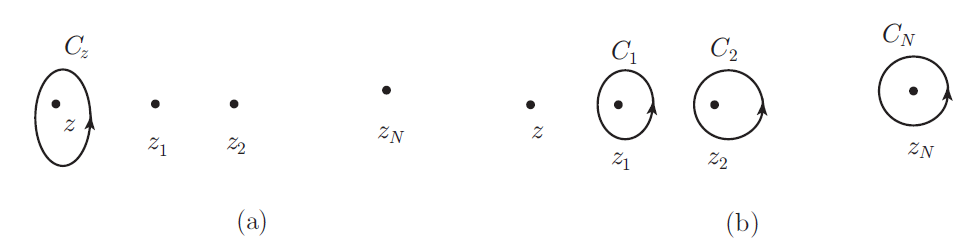
\includegraphics[width=0.6\linewidth]{fig/4.1.png}
	\caption{ (a)围绕$z$的闭合曲线,(b)围绕$z_1, \cdots, z_N$的闭合曲线。}
\end{figure}

右边用 $T(\zeta)$ 和 $\phi_i(z_i)$ 的OPE写成
\begin{equation}
	-\sum_{i=1}^{N} \int_{C_{i}} \frac{d \zeta}{2 \pi i}(\zeta-z)^{1-n}\left(\frac{h_{i}}{\left(\zeta-z_{i}\right)^{2}}+\frac{1}{\zeta-z_{i}} \partial_{i}\right)\left\langle\phi(z) \phi_{1}\left(z_{1}\right) \cdots \phi_{N}\left(z_{N}\right)\right\rangle
\end{equation}
计算$ \zeta=z_i $处的留数,得到
\begin{equation}
	\left\langle\left(L_{-n} \phi\right)(z) \phi_{1}\left(z_{1}\right) \cdots \phi_{N}\left(z_{N}\right)\right\rangle=\mathcal{L}_{-n}\left\langle\phi(z) \phi_{1}\left(z_{1}\right) \cdots \phi_{N}\left(z_{N}\right)\right\rangle
\end{equation}
其中
\begin{equation}
	\mathcal{L}_{-n}=\sum_{i=1}^{N}\left[\frac{(n-1) h_{i}}{\left(z_{i}-z\right)^{n}}-\frac{1}{\left(z_{i}-z\right)^{n-1}} \partial_{i}\right]
\end{equation}
重复这样的操作可得到
\begin{equation}
	\left\langle\left(L_{-n_{1}} \cdots L_{-n_{k}} \phi\right)(z) \phi_{1}\left(z_{1}\right) \cdots \phi_{N}\left(z_{N}\right)\right\rangle = \mathcal{L}_{-n_{1}} \cdots \mathcal{L}_{-n_{k}}\left\langle\phi(z) \phi_{1}\left(z_{1}\right) \cdots \phi_{N}\left(z_{N}\right)\right\rangle
\end{equation}
这样,计算包含次级场的关联函数,就转换成计算只包含初级场的关联函数。

\section{OPE的自举}
在共形场论中,Virasoro代数作用在局域场的空间上,初级场的共形类中的元素同Virasoro代数的Verma模中的元素一一对应。这个场的空间记作 $\mathcal{A}$ ,$ \mathcal{A}$ 是Virasoro代数的可约表示。将 $\mathcal{A} $分解成Virasoro代数的不可约表示,各不可约表示中有一个最高权向量,对应一个初级场。因此,局域场的空间 $\mathcal{A} $是初级场的共形类的直和,可分解成
$$
\mathcal{A}=\oplus_{\ell}\left[\phi_{\ell}\right]
$$
指标 $\ell$ 或离散,或连续。

场论中一个重要想法是自举(bootstrap)。这是由Polyakov\footnote{A. M. Polyakov, Sov. Phys. JETP 30 (1970) 151.},Kadanoff\footnote{L. P. Kadanoff, Phys. Rev. Lett. 23 (1969) 1430.}和Wilson\footnote{K. G. Wilson, Phys. Rev. 179 (1969) 1499.}提出的,同时提出的还有算符乘积展开和重整化群的想法。这一想法下,定义关联函数不是通过基本场 $\varphi(x) $的路径积分,而是通过$ \varphi(x) $和它的(包含导数的)复合场$ \varphi^{n_{0}}(\partial \varphi)^{n_{1}} \cdots$ 整体组成的局域场$ A_i(x) $的关联函数间的关系。局域场全体构成的空间 $\mathcal{A}$ 是完备集,也就是说,任何局域场都可写成 $\mathcal{A}$ 的基$ A_i(x)$ 的线性组合。那么,局域场 $A_i(x) $和 $A_j(y) $的算符乘积,就可在两点 $x,y$ 趋近时用 $\mathcal{A}$ 中的元素展开成
$$
A_{i}(x) A_{j}(y)=\sum_{k} C_{i j}^{k}(x, y) A_{k}(y)
$$
在二维共形场论中,初级场的共形类构成了局域场的完备集。可对初级场 $\phi_1(z,\bar{z})$ 和 $\phi_2(0,0)$ 的OPE作共形类分解:
\begin{equation}
	\phi_{1}(z, \bar{z}) \phi_{2}(0,0)=\sum_{k} C_{12}^{k} z^{-h_{1}-h_{2}+h_{k}} \bar{z}^{-\bar{h}_{1}-\bar{h}_{2}+\bar{h}_{k}} \Psi_{k}(z, \bar{z})
\end{equation}
这里,$ C_{12}^{k} $是常数,$ \Psi_{k}(z, \bar{z}) $可用共形类$ [\phi_k] $中的元素展开成
\begin{equation}
	\Psi_{k}(z, \bar{z})=\phi_{k}(0,0)+\beta_{1} z L_{-1} \phi_{k}(0,0)+\bar{\beta}_{1} \bar{z} \bar{L}_{-1} \phi_{k}(0,0)+\cdots
\end{equation}
这里作了归一化,以使$ \phi_{k}(0,0)$ 项的系数为1。因为Virasoro算符的右模 $L_{-n} $和左模$ \bar{L}_{-m}$ 独立地作用, $\Psi_{k}$ 对应的态 $|\Psi_{k}\rangle $可写成张量积
$$
\left|\Psi_{k}\right\rangle=\left|\psi_{k}\right\rangle \otimes |\bar{\psi}_{k} \rangle
$$
$\left|\psi_{k}\right\rangle$ 可展开成
\begin{equation}
	\left|\psi_{k}\right\rangle=\sum_{\{n\}} \beta_{12}^{k\{n\}} L_{-n_{1}} \cdots L_{-n_{p}}\left|\phi_{k}\right\rangle
\end{equation}
这里, $\{n\} $指非负整数的集合,其中的元素满足$ n_{1} \geq \cdots \geq n_{p}>0 $, $\beta_{12}^{k\{n\}} $是常数。相应地, $\Psi_{k}(z, \bar{z})$ 可写成
\begin{equation}
\begin{aligned} \Psi_{k}(z, \bar{z})=& \sum_{\{n\},\{m\}} \beta_{12}^{k\{n\}} \bar{\beta}_{12}^{k\{m\}} z^{\sum_{i} n_{i}} \bar{z}^{\sum_jm_{j}} \\ & \times L_{-n_{1}} \cdots L_{-n_{p}} \bar{L}_{-m_{1}} \cdots \bar{L}_{-m_{q}} \phi_{k}(0,0) \end{aligned}
\end{equation}
OPE (4.38) 作用在 $SL(2,\mathbb{C}) $不变真空$ |0\rangle$ 上,可以确定 $\beta,\bar{\beta} $:
\begin{equation}
	\phi_{1}(z, \bar{z}) \phi_{2}(0,0)|0\rangle=\sum_{k} C_{12}^{k} z^{-h_{1}-h_{2}+h_{k}} \bar{z}^{-\bar{h}_{1}-\bar{h}_{2}+\bar{h}_{k}}\left|\Psi_{k}(z, \bar{z})\right\rangle
\end{equation}
考虑$ L_n $( $n\geq 0 $)生成的无穷小共形变换。左边作用上$ L_n $得到
\begin{equation}
	L_{n}\left(\phi_{1}(z, \bar{z}) \phi_{2}(0,0)\right)|0\rangle=\left(\left[L_{n}, \phi_{1}(z, \bar{z})\right] \phi_{2}(0,0)+\phi_{1}(z, \bar{z})\left[L_{n}, \phi_{2}(0,0)\right]\right)|0\rangle
\end{equation}
因为$ L_n $对 $\phi_i(z,\bar{z}) $( $i=1,2 $)生成的无穷小变换是
\begin{equation}
	\left[L_{n}, \phi_{i}(z, \bar{z})\right]=z^{n+1} \partial \phi_{i}(z, \bar{z})+h_{i}(n+1) z^{n} \phi_{i}(z, \bar{z})
\end{equation}
$n>0$ 时有
\begin{equation}
L_{n}\left(\phi_{1}(z, \bar{z}) \phi_{2}(0,0)\right)|0\rangle=\left(\left(z^{n+1} \partial_{z}+h_{1}(n+1) z^{n}\right) \phi_{1}(z, \bar{z})\right) \phi_{2}(0,0)|0\rangle	
\end{equation}
$n=0 $时有
\begin{equation}
L_{0}\left(\phi_{1}(z, \bar{z}) \phi_{2}(0,0)\right)|0\rangle=\left(z \partial_{z}+h_{1}+h_{2}\right) \phi_{1}(z, \bar{z}) \phi_{2}(0,0)|0\rangle	
\end{equation}
由此知道 $|\psi_k\rangle$ 满足
\begin{align}
	L_{n} z^{-h_{1}-h_{2}+h_{k}}\left|\psi_{k}\right\rangle=&\left(z^{n+1} \partial_{z}+(n+1) h_{1} z^{n}\right) z^{-h_{1}-h_{2}+h_{k}}\left|\psi_{k}\right\rangle, \quad n>0,\\ L_{0} z^{-h_{1}-h_{2}+h_{k}}\left|\psi_{k}\right\rangle=&\left(z \partial_{z}+h_{1}+h_{2}\right) z^{-h_{1}-h_{2}+h_{k}}\left|\psi_{k}\right\rangle 
\end{align}
$|\psi_k\rangle$ 可展开成
\begin{equation}
	\left|\psi_{k}\right\rangle=\sum_{N=0}^{\infty} z^{N}\left|h_{k}, N\right\rangle
\end{equation}
例如\footnote{[这里记号有点混乱,$\ket{h_k}$在这里应该理解为共形权为$h_k$的初级态,也就是前面的$\ket{\phi_k}$]}
\begin{align} \left|h_{k}, 0\right\rangle &=\left|h_{k}\right\rangle \\ \left|h_{k}, 1\right\rangle &=\beta_{12}^{k\{1\}} L_{-1}\left|h_{k}\right\rangle \\ \left|h_{k}, 2\right\rangle &=\left(\beta_{12}^{k\{1,1\}} L_{-1}^{2}+\beta_{12}^{k\{2\}} L_{-2}\right)\left|h_{k}\right\rangle  \end{align}
(4.49) 代入 (4.47),(4.48) 。代入 (4.48) 得到的式子显然成立。代入 (4.47) 得到
\begin{equation}
	L_{n}\left|\psi_{k}\right\rangle=\sum_{N=0}^{\infty} z^{n+N}\left(N-h_{1}-h_{2}+h_{k}+(n+1) h_{1}\right)\left|h_{k}, N\right\rangle
\end{equation}
由此知道$ |h_k,N\rangle $满足
\begin{equation}
	L_{n}\left|h_{k}, N+n\right\rangle=\left(N+n h_{1}-h_{2}+h_{k}\right)\left|h_{k}, N\right\rangle
\end{equation}
于是可以看到,系数$ \beta_{12}^{k\{n\}}$ 可以递归地确定,并表示成中心荷$ c $和共形权的函数。

我们来具体确定低阶的 $\beta_{12}^{k\{n\}}$ 。 $n=1,N=0$ 时有
\begin{equation}
L_{1}\left|h_{k}, 1\right\rangle=\left(h_{k}+h_{1}-h_{2}\right)\left|h_{k}\right\rangle 
\end{equation}
进而得到
\begin{equation}
	2 h_{k} \beta_{12}^{k\{1\}}=h_{k}+h_{1}-h_{2}
\end{equation}
$n=2,N=0 $和 $n=1,N=1$ 时则可得到
\begin{equation}
\left(\begin{array}{cc} 2\left(2 h_{k}+1\right) & 3 \\ 6 h_{k} & 4 h_{k}+\frac{c}{2} \end{array}\right)\left(\begin{array}{c} \beta_{12}^{k\{1,1\}} \\ \beta_{12}^{k\{2\}} \end{array}\right)=\left(\begin{array}{c} \left(h_{k}+h_{1}-h_{2}+1\right) \beta_{12}^{k\{1\}} \\ h_{k}+2 h_{1}-h_{2} \end{array}\right)
\end{equation}

对一般的 $c,h_k $,上式左边的矩阵是可逆的, $\beta_{12}^{k\{1,1\}},\beta_{12}^{k\{2\}} $被唯一确定。然而,有些特殊情形下,矩阵不可逆,下章再说。

\section{交叉对称性}
上节说到,初级场$ \phi_1,\phi_2$ 的OPE中 $\Psi_k$ 的结构,可通过作无穷小共形变换来确定。但前面的系数 $C_{12}^k$ ,并不能从Virasoro代数的作用确定。如果要求初级场的OPE代数满足结合律 $\left(A_{i} A_{j}\right) A_{k}=A_{i}\left(A_{j} A_{k}\right) $,可以得到$ C_{ij}^k$ 满足的非线性条件。这说明,初级场的四点函数具有某种对称性(交叉对称性)。

考虑初级场的四点函数
\begin{equation}
	\left\langle\phi_{1}\left(z_{1}, \bar{z}_{1}\right) \phi_{2}\left(z_{2}, \bar{z}_{2}\right) \phi_{3}\left(z_{3}, \bar{z}_{3}\right) \phi_{4}\left(z_{4}, \bar{z}_{4}\right)\right\rangle
\end{equation}
全局的$ SL(2,\mathbb{C}) $共形变换,可用于固定初级场4个位置 $z_1,z_2,z_3,z_4 $中的3个。例如,作共形变换
\begin{equation}
	w=\frac{\left(z_{2}-z_{1}\right)\left(z-z_{4}\right)}{\left(z_{2}-z_{4}\right)\left(z-z_{1}\right)}
\end{equation}
这将点 $(z_1,z_2,z_3,z_4)$ 映到$ (\infty,1,x,0) $,其中
\begin{equation}
x=\frac{z_{21}z_{ 34}}{z_{24} z_{31}}
\end{equation}
是交比, $z_{ij}=z_i-z_j $。关联函数按Ward恒等式 (3.3) 变换。导数是
\begin{equation}
\frac{d w}{d z}=\frac{z_{21} z_{41}}{z_{24}} \frac{1}{\left(z-z_{1}\right)^{2}}
\end{equation}
在 $z=z_2,z_3,z_4$ 处分别是
\begin{equation}
	\begin{aligned} \left.\frac{d w}{d z}\right|_{z=z_{2}} & =\frac{z_{41}}{z_{24} z_{21}} \\ \left.\frac{d w}{d z}\right|_{z=z_{3}} & =\frac{z_{21} z_{41}}{z_{24} z_{31}^{2}} \\ \left.\frac{d w}{d z}\right|_{z=z_{4}} & =\frac{z_{21}}{z_{24} z_{41}} \end{aligned}
\end{equation}
$z=z_1$ 处是发散的,不过可以考虑取极限 $z=z_1'\to z_1 $,我们有
\begin{equation}
	\left.\frac{d w}{d z}\right|_{z=z_{1}^{\prime}}=\frac{z_{21} z_{41}}{z_{24}} \frac{1}{\left(z_{1}^{\prime}-z_{1}\right)^{2}} \sim \frac{z_{24}}{z_{21} z_{41}}\left(w_{1}^{\prime}\right)^{2}
\end{equation}
其中$w_1' $是 $z=z_1'$ 处 $w$ 的值。因此四点函数可写成
\begin{equation}
	\begin{aligned} &\left\langle\phi_{1}\left(z_{1}, \bar{z}_{1}\right) \phi_{2}\left(z_{2}, \bar{z}_{2}\right) \phi_{3}\left(z_{3}, \bar{z}_{3}\right) \phi_{4}\left(z_{4}, \bar{z}_{4}\right)\right\rangle \\ =&\left(\frac{z_{24}}{z_{21} z_{41}}\right)^{h_{1}}\left(\frac{z_{41}}{z_{24} z_{21}}\right)^{h_{2}}\left(\frac{z_{21} z_{41}}{z_{24} z_{31}^{2}}\right)^{h_{3}}\left(\frac{z_{21}}{z_{24} z_{41}}\right)^{h_{4}} \\ &\times\left(\frac{\bar{z}_{24}}{\bar{z}_{21} \bar{z}_{41}}\right)^{\bar{h}_{1}}\left(\frac{\bar{z}_{41}}{\bar{z}_{24} \bar{z}_{21}}\right)^{\bar{h}_{2}}\left(\frac{\bar{z}_{21} \bar{z}_{41}}{\bar{z}_{24} \bar{z}_{31}^{2}}\right)^{\bar{h}_{3}}\left(\frac{\bar{z}_{21}}{\bar{z}_{24} \bar{z}_{41}}\right)^{\bar{h}_{4}} G^{21}_{43}(x, \bar{x}) \end{aligned}
\end{equation}
其中\footnote{[原文的记号容易引起误会,这里进行了更正]}
\begin{equation}
	\begin{aligned} G_{43}^{21}(x, \bar{x}) &=\lim _{w_{1}', \bar{w}_{1}' \rightarrow \infty}\left(w_{1}^{\prime}\right)^{2 h_{1}}\left(\bar{w}_{1}^{\prime}\right)^{2 \bar{h}_{1}}\left\langle\phi_{1}\left(w_{1}^{\prime}, \bar{w}_{1}^{\prime}\right) \phi_{2}(1,1) \phi_{3}(x, \bar{x}) \phi_{4}(0,0)\right\rangle \\ &=\bra{\phi_1} \phi_{2}(1,1) \phi_{3}(x, \bar{x})\ket{\phi_4} \end{aligned}
\end{equation}
我们引入$ Y_{43}^{21}(x, \bar{x}) $:
\begin{equation}
	G_{43}^{21}(x, \bar{x})=x^{\frac{h}{3}-h_{3}-h_{4}}(1-x)^{\frac{h}{3}-h_{2}-h_{3}} \bar{x}^{\frac{\bar{h}}{3}-\bar{h}_{3}-\bar{h}_{4}}(1-\bar{x})^{\frac{\bar{h}}{3}-\bar{h}_{2}-\bar{h}_{3}} Y_{43}^{21}(x, \bar{x})
\end{equation}
这样,四点函数可写成简单的形式
\begin{equation}
	\left\langle\phi_{1}\left(z_{1}, \bar{z}_{1}\right) \phi_{2}\left(z_{2}, \bar{z}_{2}\right) \phi_{3}\left(z_{3}, \bar{z}_{3}\right) \phi_{4}\left(z_{4}, \bar{z}_{4}\right)\right\rangle=\prod_{i<j}\left(z_{i j}\right)^{\gamma_{i j}}\left(\bar{z}_{i j}\right)^{\bar{\gamma}_{i j}} Y_{43}^{21}(x, \bar{x})
\end{equation}
其中
\begin{equation}
	\begin{aligned} &\gamma_{i j}=\frac{h}{3}-h_{i}-h_{j}, \quad h=h_{1}+h_{2}+h_{3}+h_{4}\\ &\bar{\gamma}_{i j}=\frac{\bar{h}}{3}-\bar{h}_{i}-\bar{h}_{j}, \quad \bar{h}=\bar{h}_{1}+\bar{h}_{2}+\bar{h}_{3}+\bar{h}_{4} \end{aligned}
\end{equation}

考虑另一个 $SL(2,\mathbb{C}) $变换,我们在 $z_1,z_2,z_3,z_4$ 中选取不同于上面例子的3个点,映到$ 0,1,\infty $。例如$ z_1 $映到 $\infty$ , $z_2 $映到 0 , $z_4 $映到 1 ,也就是交换初级场 $\phi_2,\phi_4$ ,那么作变换
\begin{equation}
	w=\frac{\left(z_{4}-z_{1}\right)\left(z-z_{2}\right)}{\left(z_{4}-z_{2}\right)\left(z-z_{1}\right)}
\end{equation}
这时, $z=z_3 $处的值是
\begin{equation}
	w_{3}=\frac{z_{41} z_{32}}{z_{42} z_{31}}=1-x
\end{equation}
四点函数可写成
\begin{equation}
	\begin{aligned} &\left\langle\phi_{1}\left(z_{1}, \bar{z}_{1}\right) \phi_{2}\left(z_{2}, \bar{z}_{2}\right) \phi_{3}\left(z_{3}, \bar{z}_{3}\right) \phi_{4}\left(z_{4}, \bar{z}_{4}\right)\right\rangle \\ =&\left(\frac{z_{42}}{z_{41} z_{21}}\right)^{h_{1}}\left(\frac{z_{21}}{z_{42} z_{41}}\right)^{h_{4}}\left(\frac{z_{41} z_{21}}{z_{42} z_{31}^{2}}\right)^{h_{3}}\left(\frac{z_{41}}{z_{42} z_{21}}\right)^{h_{2}} \\ & \times\left(\frac{\bar{z}_{42}}{\bar{z}_{41} \bar{z}_{21}}\right)^{\bar{h}_{1}}\left(\frac{\bar{z}_{21}}{\bar{z}_{42} \bar{z}_{41}}\right)^{\bar{h}_{4}}\left(\frac{\bar{z}_{41} \bar{z}_{21}}{\bar{z}_{42} \bar{z}_{31}^{2}}\right)^{\bar{h}_{3}}\left(\frac{\bar{z}_{41}}{\bar{z}_{42} \bar{z}_{21}}\right)^{\bar{h}_{2}} G_{23}^{41}(1-x, 1-\bar{x}) \end{aligned}
\end{equation}
比对 (4.64) 和 (4.71) 可知,差一个相位因子的意义上有
\begin{equation}
	G_{43}^{21}(x, \bar{x})=G_{23}^{41}(1-x, 1-\bar{x})
\end{equation}
再考虑 $z_1 $映到 0 , $z_2 $映到 1 , $z_4 $映到 $\infty$,那么作变换
\begin{equation}
	w=\frac{\left(z_{2}-z_{4}\right)\left(z-z_{1}\right)}{\left(z_{2}-z_{1}\right)\left(z-z_{4}\right)}
\end{equation}
这时$ z_3 $映到$ 1/x$ 。同理可得
\begin{equation}
	G_{43}^{21}(x, \bar{x})=x^{-2 h_{3}} \bar{x}^{-2 \bar{h}_{3}} G_{13}^{24}\left(1/x, 1/\bar{x}\right)
\end{equation}
关联函数 $G_{n m}^{l k}(x, \bar{x}) $间的关系 (4.72),(4.74) 是从四点函数的全局共形对称性推出的,这称为四点函数的\textbf{交叉对称性(crossing symmetry)}。

我们来用OPE计算$ G_{43}^{21}(x, \bar{x})$ 。代入 $\phi_3(x,\bar{x})$ 和 $\phi_4(0,0) $的OPE,得到
\begin{equation}
	G_{43}^{21}(x, \bar{x})=\sum_{p} C_{43}^{p} C_{12}^{p} A_{43}^{21}(p | x, \bar{x})
\end{equation}
其中
\begin{equation}
	A_{43}^{21}(p | x, \bar{x})=\left(C_{12}^{p}\right)^{-1} x^{h_{p}-h_{3}-h_{4}} \bar{x}^{\bar{h}_{p}-\bar{h}_{3}-\bar{h}_{4}}\left\langle\phi_{1}\left|\phi_{2}(1,1) \Psi_{p}(x, \bar{x})\right| 0\right\rangle
\end{equation}
$A_{43}^{21}(p | x, \bar{x}) $可进一步分解成
\begin{equation}
	A_{43}^{21}(p | x, \bar{x})=F_{43}^{21}(p| x) \bar{F}_{43}^{21}(p | \bar{x})
\end{equation}
其中\footnote{[这里用到了,$C_{12}^p=\left\langle\phi_{1}\left|\phi_{2}(1,1)\right| \phi_{p}\right\rangle$,详见大黄书P181.]}
\begin{equation}
	F_{43}^{21}(p |x)=x^{h_{p}-h_{3}-h_{4}} \sum_{\{n\}} \beta_{43}^{p\{n\}}x^{\sum_{i=1}^{k} n_{i}} \frac{\left\langle\phi_{1}\left|\phi_{2}(1,1) L_{-n_{1}} \cdots L_{-n_{k}}\right| \phi_{p}\right\rangle}{\left\langle\phi_{1}\left|\phi_{2}(1,1)\right| \phi_{p}\right\rangle}
\end{equation}
因此,$F_{43}^{21}(p |x)$ 是构造四点函数的基础材料,称为\textbf{共形块(conformal block)}。

交叉对称性 (4.72) 成为
\begin{equation}
	\sum_{p} C_{43}^{p} C_{12}^{p} F_{43}^{21}(p | x) \bar{F}_{43}^{21}(p | \bar{x})=\sum_{q} C_{32}^{p} C_{14}^{q} F_{32}^{41}(q | 1-x) \bar{F}_{32}^{41}(q | 1-\bar{x})
\end{equation}
如果算出共形块,这就给出OPE系数 $C_{n m}^{l} $和共形权 $h_i $的方程。通过求解它,可以考察CFT的关联函数。这个方程是非线性的,很难求解,不过人们已经详细研究了极小模型的结构。

\chapter{极小模型}
本章考虑Virasoro代数的退化表示,并介绍零模向量。所有初级场都是二重退化表示的CFT称为极小模型,是二维CFT中最基本的。极小模型中,退化初级场的关联函数满足解有固定奇点的微分方程,解它可得到共形块。此外,利用单值变换下的不变性,可以得到对关联函数的约束,算出OPE系数。我们也会解释由Dotsenko-Fateev提出的极小模型的自由场表示,这是推导关联函数的积分表示的系统方法。

\section{Virasoro代数的退化表示}
共形场论局域场的空间 $\mathcal{A} $是初级场$ \phi_i$ 所属的共形类$ [\phi_i]$ 的直和: $\mathcal{A}=\oplus_{i}\left[\phi_{i}\right]$ 。如果 $\phi_i$ 的共形权是 $(h_i,\bar{h}_i) $,共形类$ [\phi_i] $就可写成Virasoro代数右模( $L_n$ )和左模( $\bar{L}_n$ )的表示 $V_{h_{i}}, \bar{V}_{\bar{h}_{i}} $的张量积: $\left[\phi_{i}\right]=V_{h_{i}} \otimes \bar{V}_{\bar{h}_{i}} $。这里用了态-算符对应,将场和Hilbert空间中的态视作等同。Verma模 $V_h$ 由最高权态 $|h\rangle$ 和它的次级态 $L_{-n_{1}} \cdots L_{-n_{k}}|h\rangle$ ( $n_{1} \geq \cdots \geq n_{k}>0$ )生成。最高权态 $|h\rangle$ 满足 $L_{n}|h\rangle=0(n>0) $, $L_{0}|h\rangle=h|h\rangle $。

Verma模$ V_h $未必是Virasoro代数的不可约表示,也可能是不可约表示之和。有Verma模 $V_h$ 的元素$ |h+N\rangle$ ( N 是正整数)满足
\begin{align} &L_{n}|h+N\rangle=0, \quad n>0 \\ &L_{0}|h+N\rangle=(h+N)|h+N\rangle \end{align}
时,$ L_{-n} $作用在 $|h+N\rangle $上生成的空间 $V_{h+N}$ 是Virasoro代数的表示空间。这个态$ |h+N\rangle$ 称为级为 $N $的\textbf{零模向量(null vector)}或\textbf{奇异向量(singular vector)}。对应零模向量的共形场称为\textbf{零模场(null field)}。如果 $|h+N\rangle $是级为 N 的零模向量,Verma模中任何元素 $L_{-n_{1}} \cdots L_{-n_{k}}|h\rangle $与它的内积将是
\begin{equation}
	\left\langle h+N\left|L_{-n_{1}} \cdots L_{-n_{k}}\right| h\right\rangle=\left\langle h\left|L_{n_{k}} \cdots L_{n_{1}}\right| h+N\right\rangle^{*}=0
\end{equation}
特别地,它自身的范数为零: $\langle h+N | h+N\rangle=0 $。$ |h+N\rangle$ 的次级态同样与所有Verma模中元素正交。

如果Virasoro代数的表示 $V_h$ 不可约,$ V_h $就不包含零模向量。同样地,如果 $V_h$ 不包含零模向量,它就是不可约表示。$ V_h $包含一个零模向量 $|h+N\rangle$ 时, $V_h $中定义等价关系
\begin{equation}
	|h+N\rangle=0
\end{equation}
得到的空间 $[h]$ (商空间$ V_h/V_{h+N}$ )是Virasoro代数的不可约表示。这个表示 $[h]$ 称为\textbf{退化表示(degenerate representation)},$ N $称为退化表示的级。

\subsection{零模向量的组成}
Virasoro代数的最高权表示是退化表示时,可以得到共形权 $h $和中心荷$c$ 间的关系。我们构造具体的零模向量来考察这个关系。Verma模$ V_h$ 中级为 $N$ 的态可写成
$$
L_{-n_{1}} \cdots L_{-n_{k}}|h\rangle, \quad n_{1} \geq \cdots \geq n_{k}>0 \quad (N=n_{1}+\cdots+n_{k})
$$
的线性组合。

例如级为1的态形如
\begin{equation}
	|\chi\rangle=L_{-1}|h\rangle
\end{equation}
假定它是零模向量,那么作用上 $L_n$ ( $n>0 $)有
\begin{equation}
\begin{aligned} L_{n}|\chi\rangle &=L_{n} L_{-1}|h\rangle=\left(\left[L_{n}, L_{-1}\right]+L_{-1} L_{n}\right)|h\rangle \\ &=(n+1) L_{n-1}|h\rangle \\ &=0 \end{aligned}
\end{equation}
这里,我们用了Virasoro代数和$ |h\rangle $是最高权态。 $n>1$ 时,由$ |h\rangle$ 是最高权态,右边为零。$ n=1 $时,得到
$$
2 h|h\rangle=0
$$
也就是 $h=0 $。换句话说,级为1的零模向量是 $SL(2,\mathbb{C}) $不变真空 $|0\rangle $,对应的零模场是恒等算符$ \boldsymbol{I}(z) $。
级为2的态形如
\begin{equation}
|\chi\rangle=\left(L_{-2}+a L_{-1}^{2}\right)|h\rangle
\end{equation}
这里 $a$ 是常数。假定它是零模向量,用Virasoro代数,作用上$ L_n$ ( $n>0 $)有
\begin{equation}
	\begin{aligned} L_{n}|\chi\rangle=&\left(\left[L_{n}, L_{-2}\right]+a [L_{n}, L_{-1}^{2} ]\right)|h\rangle \\ =&\left\{(n+2) L_{n-2}+\frac{c}{12}\left(n^{3}-n\right) \delta_{n-2,0}+a(n+1)\left(n L_{n-2}+2 L_{-1} L_{n-1}\right)\right\}|h\rangle \\ =& 0 \end{aligned}
\end{equation}
$n=1$ 时,得到
\begin{equation}
	L_{1}|\chi\rangle=(3+2 a(2 h+1)) L_{-1}|h\rangle=0
\end{equation}
$h=0$ 时, $L_{-1}|h\rangle $是级为1的零模向量,这等式成立。 $h\neq 0 $时,得到
\begin{equation}
	a=-\frac{3}{2(2 h+1)}
\end{equation}
$n=2 $时,得到
\begin{equation}
L_{2}|\chi\rangle=\left(4 h+\frac{c}{2}+6 a h\right)|h\rangle=0
\end{equation}
于是有关于 $h,c $的方程
\begin{equation}
	(6 a+4) h+\frac{c}{2}=0
\end{equation}
代入 (5.10) 得到 $h,c$ 间的关系
\begin{equation}
	8 h^{2}+(c-5) h+\frac{c}{2}=0
\end{equation}
$n\geq 3$ 时不会得到新等式。总结一下,$ h,c $满足 (5.13) 时,
\begin{equation}
	\left(L_{-2}-\frac{3}{2(2 h+1)} L_{-1}^{2}\right)|h\rangle
\end{equation}
是级为2的零模向量。 (5.13) 是关于 $h$ 的二次方程,对给定中心荷 $c$ ,$ h $有两取值
\begin{equation}
	h=\frac{5-c \pm \sqrt{c^{2}-26 c+25}}{16}
\end{equation}
级为3的态形如
\begin{equation}
	|\chi\rangle=\left(L_{-3}+a L_{-2} L_{-1}+b L_{-1}^{3}\right)|h\rangle
\end{equation}
这里 $a,b $是常数。假定它是零模向量,作用上Virasoro算符$ L_n $( $n>0$ )有
\begin{equation}
	\begin{aligned} L_{n}|\chi\rangle=&\Big\{(n+3) L_{n-3}+\frac{c}{12}\left(n^{3}-n\right) \delta_{n-3,0} \\ &+a \big[(n+2)(n-1) L_{n-3}+(n+1) L_{-2} L_{n-1} \\ &\quad +(n+2) L_{-1} L_{n-2}+\frac{c}{12} (n^{3}-n ) \delta_{n-2,0} L_{-1} \big] \\ &+b(n+1) (3 n L_{-1} L_{n-2}+n(n-1) L_{n-3} +3 L_{-1}^{2} L_{n-1} ) \Big\}|h\rangle \\=&0 \end{aligned}
\end{equation}
$n=1 $时,得到
\begin{equation}
	L_{1}|\chi\rangle=\left\{(4+2 a h) L_{-2}+(3 a+3 b(2 h+2)) L_{-1}^{2}\right\}|h\rangle=0
\end{equation}
于是
\begin{equation}
	4+2 a h=0, \quad 3 a+6 b(h+1)=0
\end{equation}
$n=2 $时,得到
\begin{equation}
	5+a\left(4+4 h+\frac{c}{2}\right)+3 b(6 h+2)=0
\end{equation}
$n=3$ 时,得到
\begin{equation}
	6 h+2 c+10 a h+24 b h=0
\end{equation}
这最后一个等式是多余的,只需要前三个等式。可以得到级为3的零模向量是
\begin{equation}
\left(L_{-3}-\frac{2}{h} L_{-2} L_{-1}+\frac{1}{h( h+1)} L_{-1}^{3}\right)|h\rangle
\end{equation}
其中
\begin{equation}
	h=\frac{7-c \pm \sqrt{c^{2}-26 c+25}}{6}
\end{equation}
从级为2和3的例子中可以看到,零模向量对应的共形权有特别的形式。引入参数
\begin{equation}
\alpha_{\pm}=\frac{\sqrt{1-c} \pm \sqrt{25-c}}{\sqrt{24}}
\end{equation}
$\alpha_{\pm} $满足
\begin{align} &\alpha_{+} \alpha_{-}=-1 \\ &\left(\alpha_{+}+\alpha_{-}\right)^{2}=\frac{1-c}{6}, \quad\left(\alpha_{+}-\alpha_{-}\right)^{2}=\frac{25-c}{6}  \end{align}
中心荷$ c $可用 $\alpha_{\pm} $写成
\begin{equation}
	c=1-6\left(\alpha_{+}+\alpha_{-}\right)^{2}
\end{equation}
再引入
\begin{equation}
	h_{0}=-\frac{1}{4}\left(\alpha_{+}+\alpha_{-}\right)^{2}=\frac{c-1}{24}
\end{equation}
对正整数 $n,m $定义
\begin{equation}
	h_{n, m}=h_{0}+\frac{1}{4}\left(n \alpha_{+}+m \alpha_{-}\right)^{2}
\end{equation}
$h_{n,m} $写成 $c$ 的函数是
\begin{equation}
	\begin{aligned} h_{n, m}=&\frac{1}{4}\left(n^{2}-1\right) \alpha_{+}^{2}+\frac{1}{4}\left(m^{2}-1\right) \alpha_{-}^{2}-\frac{1}{2}(m n-1) \\ =& \frac{1}{48}\Big\{-24(m n-1)+\left(n^{2}+m^{2}-2\right)(13-c)\\&+\left(n^{2}-m^{2}\right) \sqrt{(1-c)(25-c)}\Big\} \end{aligned}
\end{equation}
$n,m $较小时的几个值是
\begin{equation*}
	\begin{aligned} &h_{1,1}=0 \\& h_{1,2}=\frac{5-c-\sqrt{(1-c)(25-c)}}{16} \quad h_{2,1}=\frac{5-c+\sqrt{(1-c)(25-c)}}{16} \\& h_{1,3}=\frac{7-c-\sqrt{(1-c)(25-c)}}{6} \quad h_{3,1}=\frac{7-c+\sqrt{(1-c)(25-c)}}{6} \end{aligned}
\end{equation*}
这些共形权对应级为1, 2, 3的零模向量。

一般来说,对正整数$ n,m $,共形权$ h=h_{n,m}$ 对应级为$ N=nm $的零模向量。 (5.29) 也称为Kac谱。最高权态$ \left|h_{n, m}\right\rangle \otimes\left|h_{n, m}\right\rangle $对应的初级场记作 $\phi_{(n, m)}(z, \bar{z}) $。文献\footnote{L. Benoit and Y. Saint-Aubin, Phys. Lett. B 215 (1988) 517.}\footnote{M. Bauer, P. Di Francesco, C. Itzykson and J. B. Zuber, Nucl. Phys. B 362 (1991) 515.}中讨论了如何构造Virasoro代数的零模向量。

\section{零模场的关联函数}
考虑包含初级场 $\phi_{(n, m)}(z, \bar{z}) $的关联函数,它的共形类中有Kac谱中的零模场:
$$
\left\langle\phi_{(n, m)}(z) \phi_{1}\left(z_{1}\right) \cdots \phi_{N}\left(z_{N}\right)\right\rangle
$$
这里忽略了对 $\bar{z} $的依赖。

因为可由$ \phi_{(n, m)}(z) $得到的零模场 $\chi_{(n, m)}(z)$ 在关联函数中会给出零,可以推出关联函数需要满足的新微分方程。\footnote{由态-算符对应,两算符的关联函数正比于对应态的内积,多个算符的可通过OPE转化成两个的,而零模向量与其它态都正交,那么关联函数为零。}级为1的零模场$ \chi_{(1,1)}(z)$ 是恒等算符 $\boldsymbol{I}(z)$ ,不依赖于坐标 $z $:由 (4.17),(4.28) ,这零模场满足 $\left(L_{-1} \boldsymbol{I}\right)(z)=\partial_{z} \boldsymbol{I}(z)=0$。在关联函数中,这给出
$$
\left\langle\left(L_{-1} \boldsymbol{I}\right)(z) \phi_{1}\left(z_{1}\right) \cdots \phi_{N}\left(z_{N}\right)\right\rangle=\partial_{z}\left\langle\boldsymbol{I}(z) \phi_{1}\left(z_{1}\right) \cdots \phi_{N}\left(z_{N}\right)\right\rangle=0
$$
这等式就是在表达关联函数不依赖于 $z$ ,是平凡的。

初级场 $\phi_{(1,2)}(z) $的共形类中有级为2的零模场
\begin{equation}
	\chi_{(1,2)}(z)=\left(\left(L_{-2}-\frac{3}{2\left(2 h_{1,2}+1\right)} L_{-1}^{2}\right) \phi_{(1,2)}\right)(z)
\end{equation}
关联函数 $\left\langle\chi_{(1,2)}(z) \phi_{1}\left(z_{1}\right) \cdots \phi_{N}\left(z_{N}\right)\right\rangle $为零,由 (5.31),(4.35) 有
\begin{equation}
\begin{aligned} &\left\langle\left(\left(L_{-2}-\frac{3}{2\left(2 h_{1,2}+1\right)} L_{-1}^{2}\right) \phi_{(1,2)}\right)(z) \phi_{1}\left(z_{1}\right) \cdots \phi_{N}\left(z_{N}\right)\right\rangle \\ =&\left(\mathcal{L}_{-2}-\frac{3}{2\left(2 h_{1,2}+1\right)} \mathcal{L}_{-1}^{2}\right)\left\langle\phi_{(1,2)}(z) \phi_{1}\left(z_{1}\right) \cdots \phi_{N}\left(z_{N}\right)\right\rangle \\ =& 0 \end{aligned}
\end{equation}
代入 $\mathcal{L}_{-1}=\partial_{z}$ 以及 (4.36) 给出的 $\mathcal{L}_{-2}$ ,得到微分方程
\begin{equation}
	\begin{aligned} &\left\{\frac{3}{2\left(2 h_{1,2}+1\right)} \frac{\partial^{2}}{\partial z^{2}}-\sum_{i=1}^{N}\left[\frac{h_{i}}{\left(z-z_{i}\right)^{2}}+\frac{1}{z-z_{i}} \frac{\partial}{\partial z_{i}}\right]\right\} \\& \times\left\langle\phi_{(1,2)}(z) \phi_{1}\left(z_{1}\right) \cdots \phi_{N}\left(z_{N}\right)\right\rangle=0 \end{aligned}
\end{equation}
同样地,对共形类中有级为3的零模场的初级场$ \phi_{(1,3)}(z) $,有三阶微分方程
\begin{equation}
	\begin{aligned} &\left\{\frac{1}{ h_{1,3}+1} \frac{\partial^{3}}{\partial z^{3}}-\sum_{i=1}^{N}\left[\frac{2 h_{1,3} h_{i}}{\left(z-z_{i}\right)^{3}}+\frac{h_{1,3}}{\left(z-z_{i}\right)^{2}} \frac{\partial}{\partial z_{i}}+\frac{2 h_{i}}{\left(z-z_{i}\right)^{2}} \frac{\partial}{\partial z}+\frac{2}{z-z_{i}} \frac{\partial^{2}}{\partial z_{i} \partial z}\right]\right\} \\&\quad \times\left\langle\phi_{(1,3)}(z) \phi_{1}\left(z_{1}\right) \cdots \phi_{N}\left(z_{N}\right)\right\rangle=0 \end{aligned}
\end{equation}

一般来说,共形类中有级为$ N=nm$ 的零模场的退化初级场 $\phi_{(n, m)} $满足一个 $nm $阶微分方程。这些微分方程是Virasoro代数退化表示给出的关联函数的新约束。

\subsection{四点函数}
例如,考虑四点函数 $\left\langle\phi_{(1,2)}(z) \phi_{1}\left(z_{1}\right) \phi_{2}\left(z_{2}\right) \phi_{3}\left(z_{3}\right)\right\rangle$ 满足的微分方程。定义 $\phi_{0}\left(z_{0}\right)=\phi_{(1,2)}(z) $, $h_{0}=h_{1,2}$ ,引入交比
$$
x=\frac{z_{01} z_{23}}{z_{02} z_{13}}, \quad z_{i j}=z_{i}-z_{j}
$$
(4.64) 变成了
\begin{equation}
\begin{aligned} &\left\langle\phi_{0}\left(z_{0}\right) \phi_{1}\left(z_{1}\right) \phi_{2}\left(z_{2}\right) \phi_{3}\left(z_{3}\right)\right\rangle \\ =&\left(\frac{z_{13}}{z_{10} z_{03}}\right)^{h_{0}}\left(\frac{z_{30}}{z_{13} z_{10}}\right)^{h_{1}}\left(\frac{z_{10} z_{30}}{z_{13} z_{20}^{2}}\right)^{h_{2}}\left(\frac{z_{10}}{z_{13} z_{30}}\right)^{h_{3}} G_{32}^{10}(x) \end{aligned}
\end{equation}
其中
\begin{equation}
	G_{32}^{10}(x)=x^{a_{1}}(1-x)^{b_{1}} H(x) 
\end{equation}
$a_{1}=h_{0}+h_{1}-h_{2}-h_{3}$ ,$ b_{1}=h_{0}-h_{1}-h_{2}+h_{3}$ , $H(x)$ 满足微分方程
\begin{equation}
\begin{aligned} &\frac{3}{2\left(1+2 h_{0}\right)} \frac{d^{2} H(x)}{d x^{2}}+\frac{1-2 x}{x(1-x)} \frac{d H(x)}{d x} \\& -\left\{\frac{\lambda}{x(1-x)}+\frac{h_{1}}{x^{2}}+\frac{h_{3}}{(1-x)^{2}}\right\} H(x)=0 \end{aligned}
\end{equation}
其中 $\lambda=h_{0}+h_{1}-h_{2}+h_{3}$ 。\footnote{计算的中间结果可见P. Di Francesco et al., Conformal Field Theory, pp. 252-254.}

微分方程 (5.37) 是一个解有固定奇点 $x=0,1,\infty$ 的Fuchs型微分方程。记
\begin{equation}
	H(x)=x^{a_{2}}(1-x)^{b_{2}} F(x), \quad \frac{3}{2\left(1+2 h_{0}\right)}=\frac{1}{t}
\end{equation}
(5.30) 给出
$$
h_{1,2}=\frac{3}{4} \alpha_{-}^{2}-\frac{1}{2}
$$
于是
$$
\frac{3}{2\left(1+2 h_{0}\right)}=\frac{1}{\alpha_{-}^{2}}
$$
也就是$ t=\alpha_-^2 $。微分方程 (5.37) 可重写成
\begin{equation}
	\begin{aligned} &x(1-x) \frac{d^{2} F}{d x^{2}}+\left(t+2 a_{2}-2\left(t+a_{2}+b_{2}\right) x\right) \frac{d F}{d x} \\& +\Bigg\{-\left(a_{2}+b_{2}+t-\frac{1}{2}\right)^{2}+\left(t-\frac{1}{2}\right)^{2}-\left(h_{0}-h_{2}\right) t\\&\quad +\frac{a_{2}\left(a_{2}-1\right)+t a_{2}-h_{1} t}{x}+\frac{b_{2}\left(b_{2}-1\right)+t b_{2}-h_{2} t}{1-x}\Bigg\} F=0 \end{aligned}
\end{equation}
我们选取 $a_2,b_2 $以使$ 1/x,1/(1-x)$ 的系数为零,那么
\begin{equation}
	a_{2}=\frac{1-t \pm \sqrt{(t-1)^{2}+4 h_{1} t}}{2}, \quad b_{2}=\frac{1-t \pm \sqrt{(t-1)^{2}+4 h_{3} t}}{2}
\end{equation}
可以看到 $F(x)$ 满足超几何微分方程
\begin{equation}
	x(1-x) \frac{d^{2} F}{d x^{2}}+(\gamma-(\alpha+\beta+1) x) \frac{d F}{d x}-\alpha \beta F=0
\end{equation}
其中
\begin{equation}
	\begin{aligned} &\alpha=a_{2}+b_{2}+t-\frac{1}{2}+\sqrt{\left(t-\frac{1}{2}\right)^{2}-\left(h_{0}-h_{2}\right) t} \\& \beta=a_{2}+b_{2}+t-\frac{1}{2}-\sqrt{\left(t-\frac{1}{2}\right)^{2}-\left(h_{0}-h_{2}\right) t} \\& \gamma=t+2 a_{2} \end{aligned}
\end{equation}
不过, $\alpha,\beta$ 可以互换。定义参数$ \alpha$ 的函数\footnote{与 (5.41) 中的 $\alpha $无关}
\begin{equation}
	h(\alpha)=\frac{1}{4} \alpha^{2}-\frac{1}{4}\left(\alpha_{+}+\alpha_{-}\right)^{2}
\end{equation}
可将初级场 $\phi_1,\phi_2,\phi_3 $的共形权$ h_1,h_2,h_3 $写成 $h_{i}=h\left(\alpha_{i}\right) $。 $h_{0}=h_{1,2}=h\left(\alpha_{+}+2 \alpha_{-}\right) $。于是$ a_2,b_2$ 可写成
$$
a_{2}=\frac{1-t \pm \alpha_{1} \sqrt{t}}{2}, \quad b_{2}=\frac{1-t \pm \alpha_{3} \sqrt{t}}{2}
$$
简单起见取负号,我们得到
\begin{equation}
	\begin{aligned} &\alpha=\frac{1}{2}\left(1-\sqrt{t}\left(\alpha_{1}+\alpha_{2}+\alpha_{3}\right)\right) \\& \beta=\frac{1}{2}\left(1-\sqrt{t}\left(\alpha_{1}-\alpha_{2}+\alpha_{3}\right)\right) \\& \gamma=1-\alpha_{1} \sqrt{t} \end{aligned}
\end{equation}
以及
\begin{equation}
	a_{2}=h\left(\alpha_{1}-\alpha_{-}\right)-h_{1,2}-h\left(\alpha_{1}\right), \quad b_{2}=h\left(\alpha_{3}-\alpha_{-}\right)-h_{1,2}-h\left(\alpha_{3}\right)
\end{equation}
考虑超几何微分方程 (5.41) 在$ x=0 $附近的级数解
$$
F=x^{\lambda}\left(1+\sum_{n=1}^{\infty} a_{n} x^{n}\right)
$$
指数$ \lambda $满足方程
$$
\lambda^{2}+(\gamma-1) \lambda=0
$$
解得 $\lambda=0,1-\gamma $。 $\lambda=0 $的解记作$ F_1 $,称为超几何级数,定义为
\begin{equation}
	F_{1}(x)=F(\alpha, \beta, \gamma, x)=\sum_{n=0}^{\infty} \frac{(\alpha)_{n}(\beta)_{n}}{(1)_{n}(\gamma)_{n}} x^{n}
\end{equation}
其中
\begin{equation}
	\begin{array}{l} (x)_{n}=x(x+1) \cdots(x+n-1) \quad(n=1,2, \cdots)\\ (x)_{0}=1 \end{array}
\end{equation}
特别地, $(1)_{n}=n ! $。 $\lambda=1-\gamma $的解记作$ F_2 $,可用超几何级数写成
\begin{equation}
	F_{2}(x)=x^{1-\gamma} F(\alpha-\gamma+1, \beta-\gamma+1,2-\gamma, x)
\end{equation}
任何解都可写成线性组合$ F=c_{1} F_{1}+c_{2} F_{2} $。

那么关联函数$ G_{32}^{10}(x) $可用超几何级数写成
\begin{equation}
	\begin{aligned} G_{32}^{10}(x)=& c_{1} x^{a_{1}+a_{2}}(1-x)^{b_{1}+b_{2}} F(\alpha, \beta, \gamma, x) \\ &+c_{2} x^{a_{1}+a_{2}+1-\gamma}(1-x)^{b_{1}+b_{2}} F(\alpha-\gamma+1, \beta-\gamma+1,2-\gamma, x) \end{aligned}
\end{equation}
由 $a_1,b_1 $的定义以及 (5.44),(5.45) ,我们有
\begin{align} &a_{1}+a_{2}=h\left(\alpha_{1}-\alpha_{-}\right)-h_{2}-h_{3} \\& b_{1}+b_{2}=h\left(\alpha_{3}-\alpha_{-}\right)-h_{1}-h_{2}\\& a_{1}+a_{2}+1-\gamma=h\left(\alpha_{1}+\alpha_{-}\right)-h_{2}-h_{3} \end{align}
系数 $c_1,c_2$ 可由关联函数在单值变换下的不变性确定,这将在5.6节解释。各项都代表共形块。我们可从 $x$ 的幂次直接看出$ h_p $的值: (5.49) 的第一项对应 $h_{p}=h\left(\alpha_{1}-\alpha_{-}\right)$ ,第二项对应 $h_{p}=h\left(\alpha_{1}+\alpha_{-}\right)$ 。这表征了初级场 $\phi_{(1,2)}$ 和 $\phi_1 $的OPE的代数结构。这OPE的代数结构将在下节解释。

\section{融合规则}

我们来详细考察退化初级场OPE代数的结构,这是从零模场的微分方程推出的。在关联函数$ \left\langle\phi_{(1,2)}(z) \phi_{1}\left(z_{1}\right) \cdots \phi_{N}\left(z_{N}\right)\right\rangle $中,设退化初级场 $\phi_{(1,2)}(z)$ 和共形权是 $h_1 $的初级场 $\phi_1(z_1)$ 的OPE是
\begin{equation}
	\phi_{(1,2)}(z) \phi_{1}\left(z_{1}\right)=\sum_{k} C_{(1,2) 1}^{k}\left(z-z_{1}\right)^{h_{k}-h_{1}-h_{1,2}}\left[\phi_{k}\left(z_{1}\right)+\cdots\right]
\end{equation}
将这OPE代入关联函数的微分方程 (5.33) 。极限 $z\to z_1 $下最奇异的项是
\begin{equation}
\sum_{k} C_{(1,2) 1}^{k}\left\{\frac{3}{2\left(2 h_{1,2}+1\right)} \kappa_{k}\left(\kappa_{k}-1\right)-h_{1}+\kappa_{k}\right\}\left(z-z_{1}\right)^{\kappa_{k}-2}\left\langle\phi_{k}\left(z_{1}\right) \cdots\right\rangle	
\end{equation}
其中 $\kappa_{k}=h_{k}-h_{1}-h_{1,2} $。因此 $\kappa_k$ 满足
\begin{equation}
	\frac{3}{2\left(2 h_{1,2}+1\right)} \kappa_{k}\left(\kappa_{k}-1\right)-h_{1}+\kappa_{k}=0
\end{equation}
由这方程解得
\begin{equation}
h_{k}=\frac{1}{6}\left(1+6 h_{1}+2 h_{1,2} \pm \sqrt{1+24 h_{1}-8 h_{1,2}+48 h_{1} h_{1,2}+16 h_{1,2}^{2}}\right)	
\end{equation}
零模场的微分方程确定了 $h_k $的值。这个解形式复杂,但如果记$ h_1=h(\alpha)$ ,$ h_k $就可写成
\begin{equation}
	h\left(\alpha-\alpha_{-}\right), \quad h\left(\alpha+\alpha_{-}\right)
\end{equation}
共形权是$ h=h(\alpha)$ 的初级场记作$ \phi_{(\alpha)}$ 。我们只考虑OPE的结果中初级场所属的共形类,那么 $\phi_{(1,2)}$ 和 $\phi_{(\alpha)}$ 的OPE表达了如下的初级场共形类间的关系:
\begin{equation}
	\left[\phi_{(1,2)}\right]\left[\phi_{(\alpha)}\right]=\left[\phi_{\left(\alpha-\alpha_{-}\right)}\right]+\left[\phi_{\left(\alpha+\alpha_{-}\right)}\right]
\end{equation}
这称为\textbf{融合规则(fusion rule)}。$ \phi_{(2,1)} $对应的融合规则是
\begin{equation}
	\left[\phi_{(2,1)}\right]\left[\phi_{(\alpha)}\right]=\left[\phi_{\left(\alpha-\alpha_{+}\right)}\right]+\left[\phi_{\left(\alpha+\alpha_{+}\right)}\right]
\end{equation}
$\phi_{(1,2)} $同时也是 $\phi_{\left(\alpha_{+}+2 \alpha_{-}\right)} $,那么特别地, $\phi_{(1,2)}$ 和 $\phi_{(1,2)} $的融合规则是
\begin{equation}
	\left[\phi_{(1,2)}\right]\left[\phi_{(1,2)}\right]=\left[\phi_{(1,1)}\right]+\left[\phi_{(1,3)}\right]
\end{equation}

考虑融合规则的代数性质时,也称它为\textbf{融合代数(fusion algebra)}。OPE代数有结合律,那么融合规则就有结合律,自然地也有分配律。 (5.60) 两边作用在 $[\phi(\alpha)] $上。由 (5.58) ,左边是
\begin{equation}
	\begin{aligned} \left(\left[\phi_{(1,2)}\right]\left[\phi_{(1,2)}\right]\right)\left[\phi_{(\alpha)}\right] &=\left[\phi_{(1,2)}\right]\left(\left[\phi_{(1,2)}\right]\left[\phi_{(\alpha)}\right]\right) \\ &=\left[\phi_{(1,2)}\right]\left(\left[\phi_{\left(\alpha-\alpha_{-}\right)}\right]+\left[\phi_{\alpha+\alpha_{+}}\right]\right) \\ &=\left[\phi_{\left(\alpha-2 \alpha_{-}\right)}\right]+2\left[\phi_{(\alpha)}\right]+\left[\phi_{\left(\alpha+2 \alpha_{-}\right)}\right] \end{aligned}
\end{equation}
另一方面,$ \phi_{(1,1)} $是恒等算符,那么 (5.60) 的右边是
\begin{equation}
	\left[\phi_{(\alpha)}\right]+\left[\phi_{(1,3)}\right]\left[\phi_{(\alpha)}\right]
\end{equation}
这意味着
\begin{equation}
	\left[\phi_{(1,3)}\right]\left[\phi_{(\alpha)}\right]=\left[\phi_{\left(\alpha-2 \alpha_{-}\right)}\right]+\left[\phi_{(\alpha)}\right]+\left[\phi_{\left(\alpha+2 \alpha_{-}\right)}\right]
\end{equation}
重复这样的操作,可以得到 $\phi_{(1, m)} $和 $\phi_{(\alpha)}$ 的融合规则是
\begin{equation}
	\begin{aligned} \left[\phi_{(1, m)}\right]\left[\phi_{(\alpha)}\right] &=\left[\phi_{\left(\alpha+(-m+1) \alpha_{-}\right)}\right]+\left[\phi_{\left(\alpha+(-m+3) \alpha_{-}\right)}\right]+\cdots+\left[\phi_{\left(\alpha+(m-1) \alpha_{-}\right)}\right] \\ &=\sum_{l=0}^{m-1}\left[\phi_{\left(\alpha+(2 l-m+1) \alpha_{-}\right.}\right] \end{aligned}
\end{equation}
对这进行推广,一般的退化初级场 $\phi_{(n, m)}$ 和初级场$ \phi_{(\alpha)} $的融合规则是
\begin{equation}
	\left[\phi_{(n, m)}\right]\left[\phi_{(\alpha)}\right]=\sum_{k=0}^{n-1} \sum_{l=0}^{m-1}\left[\phi_{\left(\alpha+(2 k-n+1) \alpha_{+}+(2 l-m+1) \alpha_{-}\right)}\right]
\end{equation}
我们这里应当注意退化初级场间的融合规则。例如 $\phi_{(1,2)} $和 $\phi_{(2,1)}$ 的, $\phi_{(2,1)} $和 $\phi_{(1,2)}$ 的,似乎应当是
\begin{equation}
\begin{array}{l} {\left[\phi_{(1,2)}\right]\left[\phi_{(2,1)}\right] \stackrel{?}{=}\left[\phi_{(2,0)}\right]+\left[\phi_{(2,2)}\right]} \\ {\left[\phi_{(2,1)}\right]\left[\phi_{(1,2)}\right] \stackrel{?}{=}\left[\phi_{(0,2)}\right]+\left[\phi_{(2,2)}\right]} \end{array}
\end{equation}
两个融合规则应当一样,可是这里一个是 $\left[\phi_{(2,0)}\right]$ ,一个是 $\left[\phi_{(0,2)}\right] $。其实,OPE系数$ C_{(1,2)(2,1)}^{(2,0)}$ 和 $C_{(2,1)(1,2)}^{(0,2)} $为零,这里默认不是了。如果系数为零,融合代数将是
\begin{equation}
	\begin{array}{l} {\left[\phi_{(1,2)}\right]\left[\phi_{(2,1)}\right]=\left[\phi_{(2,2)}\right]} \\ {\left[\phi_{(2,1)}\right]\left[\phi_{(1,2)}\right]=\left[\phi_{(2,2)}\right]} \end{array}
\end{equation}

这样融合规则的定义是一致的。OPE系数的具体计算之后再说,这里只给出结果:不属于Kac谱,也就是共形权不是 $h_{n,m} $( $n,m $是正整数),而是例如 $h_{0,m}$ , $h_{n,0} $等的场,不会出现在融合规则的右边。那么,退化初级场 $\phi_{\left(n_{1}, m_{1}\right)}$ , $\phi_{\left(n_{2}, m_{2}\right)} $的融合规则关于Kac谱中的初级场是封闭的。例如,考虑 $\phi_{\left(1, m_{1}\right)}$ 和 $\phi_{\left(1, m_{2}\right)} $的,在 (5.64) 中令 $\alpha=\alpha_{+}+m_{2} \alpha_{-}$ 得到
\begin{equation}
	\begin{aligned} \left[\phi_{\left(1, m_{1}\right)}\right]\left[\phi_{\left(1, m_{2}\right)}\right] &=\left[\phi_{\left(1, m_{2}-m_{1}+1\right)}\right]+\cdots+\left[\phi_{\left(1, m_{2}+m_{1}-1\right)}\right] \\ & \stackrel{?}{=} \sum_{k=0}^{m_{1}-1}\left[\phi_{\left(1, m_{2}-m_{1}+2 k+1\right)}\right] \end{aligned}
\end{equation}
但融合规则的右边不会出现 $m_{2}-m_{1}+2 k+1<0 $的项。我们来考虑$ k $要满足的条件。如果 $m_{2}-m_{1} \geq 0 $,那么 $k=0, \cdots, m_{1}-1 $都行。如果 $m_{2}-m_{1}<0 $,考虑 $\phi_{\left(1, m_{1}\right)} $和 $\phi_{\left(1, m_{2}\right)} $互换后的融合规则
\begin{equation}
	\left[\phi_{\left(1, m_{2}\right)}\right]\left[\phi_{\left(1, m_{1}\right)}\right] \stackrel{?}{=} \sum_{k=0}^{m_{2}-1}\left[\phi_{\left(1, m_{1}-m_{2}+2 k+1\right)}\right]
\end{equation}
右边的场在 $k=0, \cdots, m_{2}-1$ 时都属于Kac谱。这可统一写成
\begin{equation}
	\left[\phi_{\left(1, m_{1}\right)}\right]\left[\phi_{\left(1, m_{2}\right)}\right]=\sum_{k=0}^{\min \left(m_{1}, m_{2}\right)-1}\left[\phi_{\left(1,\left|m_{1}-m_{2}\right|+2 k+1\right)}\right]
\end{equation}
$\min \left(m_{1}, m_{2}\right) $指 $m_1,m_2 $中更小的数。于是一般的退化初级场间融合规则是
\begin{equation}
	\left[\phi_{\left(n_{1}, m_{1}\right)}\right]\left[\phi_{\left(n_{2}, m_{2}\right)}\right]=\sum_{k=0}^{\min \left(n_{1}, n_{2}\right)-1 } \sum_{l=0}^{\min \left(m_{1}, m_{2}\right)-1}\left[\phi_{\left(\left|n_{1}-n_{2}\right|+2 k+1,\left|m_{1}-m_{2}\right|+2 l+1\right)}\right]
\end{equation}
这也可写成
\begin{equation}
	\left[\phi_{\left(n_{1}, m_{1}\right)}\right]\left[\phi_{\left(n_{2}, m_{2}\right)}\right]=\sum_{k=\left|n_{1}-n_{2}\right|+1}^{n_{1}+n_{2}-1} \sum_{l=\left|m_{1}-m_{2}\right|+1}^{m_{1}+m_{2}-1}\left[\phi_{(k, l)}\right]
\end{equation}
注意当$n_1+n_2$为奇数时,$k$对偶数求和,反之对奇数求和,对$l$求和同理。在初级场的OPE代数中,退化初级场的OPE是封闭的。

\section{极小模型}
在Belavin-Polyakov-Zamolodchikov的论文\footnote{A. A. Belavin, A. M. Polyakov and A. B. Zamolodchikov, Nucl. Phys. B 241 (1984) 333.}中,考虑了所有初级场都属于退化表示的共形场论。为使共形场论在物理上有意义,考虑的是Hilbert空间上内积正定,共形权非复也非负\footnote{非酉CFT中则是容许的。}的。

\begin{figure}[h]
	\centering
	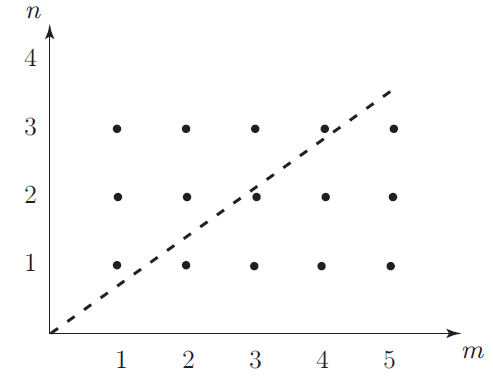
\includegraphics[width=0.6\linewidth]{fig/5.1.png}
	\caption{Kac谱的格点图。}
\end{figure}

我们来考察什么样的共形场论符合这要求。由 (5.24) ,中心荷 $c $满足$ 1<c<25$ 时,$ \alpha_\pm$ 是复的,Kac谱中的共形权 $h_{n,m}$ 一般也是复的。因此,退化初级场给出的中心荷 $c$ 有限制 $c\leq 1 $或$c\geq 25$ 。$ c\geq 25$时, $\alpha_\pm$ 是纯虚数,如果$n,m $足够大,共形权 $h_{n,m}$ 将是负的。因此考虑 $c\leq 1$ 。退化初级场的共形权由二维中坐标为$ (m,n) $的格点代表,如图5.1。虚线是斜率为
$$
\tan \theta=-\frac{\alpha_{-}}{\alpha_{+}}
$$
的直线。对一般的 $c<1 $, $\alpha_-/\alpha_+ $是无理数,虚线上没有格点。但可以看到, $(m,n)$ 取值合适时,格点可以任意接近虚线。这时,$ \left(n \alpha_{+}+m \alpha_{-}\right)^{2} $\footnote{由解析几何不难知道,这个量与点$ (n,m) $到直线$ n=-\alpha_- m/\alpha_+ $的距离正相关}可以任意小,因此存在使得 $h_{n,m}<0$ 的格点。

如果斜率是有理数呢?
\begin{equation}
\tan \theta=-\frac{\alpha_{-}}{\alpha_{+}}=\frac{q}{p}, \quad p, q \in \mathbb{Z}, \quad p>q
\end{equation}
这时, $p \alpha_{-}+q \alpha_{+}=0$ ,初级场间有了新的关系。由 (5.29) ,初级场 $\phi_{(n, m)}$ 的共形权 $h_{n,m} $满足
\begin{align} &h_{n+q, m+p}=h_{n, m}\\ &h_{q-n, p-m}=h_{n, m} \\ &h_{n, m}+n m=h_{n+q, p-m}=h_{q-n, p+m} \\ &h_{n, m}+(q-n)(p-m)=h_{n, 2 p-m}=h_{2 q-n, m} \end{align}
这说明,初级场 $\phi_{(n, m)} $的Verma模中级为$ nm$ ( $(q-n)(p-m)$ )的零模态,属于初级场 $\phi_{(n+q, p-m)}$ 或 $\phi_{(q-n, p+m)} $( $\phi_{(n, 2p-m)}$ 或 $\phi_{(2q-n, m)}$ )的Kac谱。因此, $\alpha_-/\alpha_+$ 是有理数时,初级场 $\phi_{(n, m)}$ 有级为 $nm$ 和 $(q-n)(p-m)$ 的零模场。

令零模场等价成$0$,可以得到Virasoro代数的不可约表示。可以看到,Kac谱中只剩下有限个独立的初级场,对应$ n=1,2,...,q-1$ , $m=1,2,...,p-1$ 。此外,根据对称性 (5.75) 令 $\phi_{(q-n, p-m)} $和 $\phi_{(n, m)}$ 等价,就只剩下 $(p-1)(q-1)/2 $个初级场。接着,由$ p \alpha_{-}+q \alpha_{+}=0 $和 $\alpha_{+} \alpha_{-}=-1 $解得
\begin{equation}
	\alpha_{-}=\sqrt{\frac{q}{p}}, \quad \alpha_{+}=-\sqrt{\frac{p}{q}}
\end{equation}
那么中心荷和共形权就是
\begin{align} &c=1-6\left(\alpha_{+}+\alpha_{-}\right)^{2}=1-6 \frac{(p-q)^{2}}{p q} \\ &h_{n, m}=\frac{(n p-m q)^{2}-(p-q)^{2}}{4 p q} \end{align}
一般来说,这样的共形场论中初级场是有限个,而不是通常的无穷个,称为\textbf{极小模型}。

我们来考察$ 0<n<q$ , $0<m<p$ 的格点上的初级场融合代数的具体结构。 $(p,q)=(3,2) $时,有$ \phi_{(1,1)} $和$ \phi_{(1,2)}$ ,但对称性 (5.75) 给出 $\phi_{(1,1)}=\phi_{(1,2)} $。因此这个理论中只有恒等算符 $\boldsymbol{I}=\phi_{(1,1)} $,中心荷是 $c=0$ 。非平凡的理论例如 $(p,q)=(5,2)$ 或 $(p,q)=(4,3)$ ,接下来考察一个例子。

$(p,q)=(5,2) $模型的Kac谱中,有初级场 $\phi_{(1,1)} $, $\phi_{(1,2)}$ , $\phi_{(1,3)} 和 \phi_{(1,4)}$ 。对称性给出$ \phi_{(1,3)}=\phi_{(1,2)}$ , $\phi_{(1,4)}=\phi_{(1,1)}$ 。$ \phi_{(1,2)} $的共形权是
$$
h_{1,2}=\bar{h}_{1,2}=-\frac{1}{5}
$$
中心荷是
$$
c=-\frac{22}{5}
$$
见表5.1。
\begin{table}[h]
	\centering
	\begin{tabular}{l|ccccc}
		$n$ &   &                &                &   &     \\
		1   & 0 & $-\frac{1}{5}$ & $-\frac{1}{5}$ & 0 &     \\ \hline
		& 1 & 2              & 3              & 4 & $m$
	\end{tabular}
	\caption{Yang-Lee边界奇点($c=-22/5$)的Kac谱。}
\end{table}

这个理论的Hilbert空间上内积不正定,但是一个只有恒等算符 $\boldsymbol{I}(z, \bar{z})=\phi_{(1,1)}(z, \bar{z}) $和另一个初级场 $\varphi(z, \bar{z})=\phi_{(1,2)}(z, \bar{z}) $的,很简单的共形场论。由于同二维临界现象的关联, (5,2) 极小模型也称为对应Yang-Lee边界奇点的共形场论。考虑它的融合规则。由 (5.70) , $\phi_{(1,2)}$ 自身的融合规则是
\begin{equation}
	\left[\phi_{(1,2)}\right]\left[\phi_{(1,2)}\right]=\left[\phi_{(1,1)}\right]+\left[\phi_{(1,3)}\right]
\end{equation}
$\phi_{(1,3)}=\phi_{(1,2)} $意味着
\begin{equation}
	[\varphi][\varphi]=[I]+[\varphi]
\end{equation}\quad \quad (5.82)

$\varphi $自身的融合规则还可写成
\begin{align} &\left[\phi_{(1,2)}\right]\left[\phi_{(1,3)}\right]=\left[\phi_{(1,2)}\right]+\left[\phi_{(1,4)}\right]\\ &\left[\phi_{(1,3)}\right]\left[\phi_{(1,3)}\right] \stackrel{?}{=}\left[\phi_{(1,1)}\right]+\left[\phi_{(1,3)}\right]+\left[\phi_{(1,5)}\right] \end{align}
这里,融合规则 (5.81),(5.83),(5.84) 要表达同一规则 (5.82) , (5.84) 右边 $\left[\phi_{(1,5)}\right] $的OPE系数就要为零。这样,在极小模型中初级场的融合规则中,同时有“上界”和5.3节讨论过的“下界”,融合规则在格点上封闭。

接着考虑 $(p,q)=(4,3) $的情形,这时中心荷是
$$
c=\frac{1}{2}
$$
初级场有恒等算符 $\boldsymbol{I}=\phi_{(1,1)}=\phi_{(2,3)} $,共形权为 (1/16,1/16) 的 $\sigma \equiv \phi_{(1,2)}=\phi_{(2,2)} $和共形权为 (1/2,1/2) 的 $\epsilon \equiv \phi_{(1,3)}=\phi_{(2,1)}$ ,见表5.2。 $\sigma(z, \bar{z}) $是自旋算符, $\epsilon(z, \bar{z})$ 是能量密度算符。 (4,3) 模型的中心荷和初级场的共形权都非负,Hilbert空间上的内积也是正定的。换句话说,这个CFT是酉的。在二维临界现象中,这个CFT对应Ising模型。
\begin{table}[h]
	\centering
		\begin{tabular}{l|cccc}
			$n$ &               &                &               &     \\
			2   & $\frac{1}{2}$ & $\frac{1}{16}$ & 1             &     \\
			1   & 0             & $\frac{1}{16}$ & $\frac{1}{2}$ &     \\ \hline
			& 1             & 2              & 3             & $m$
		\end{tabular}
	\caption{Ising模型(c=1/2)的Kac谱。}
\end{table}

$\sigma$ 间的融合规则同 (5,2) 模型类似:
\begin{equation}
	[\sigma][\sigma]=[I]+[\epsilon]
\end{equation}
$\epsilon $间的融合规则有两种形式:
\begin{align} &{\left[\phi_{(2,1)}\right]\left[\phi_{(2,1)}\right] \stackrel{?}{=}\left[\phi_{(1,1)}\right]+\left[\phi_{(3,1)}\right]}\\& {\left[\phi_{(1,3)}\right]\left[\phi_{(1,3)}\right] \stackrel{?}{=}\left[\phi_{(1,1)}\right]+\left[\phi_{(1,3)}\right]+\left[\phi_{(1,5)}\right] } \end{align}
这两种要表达同一规则, (5.86) 中 $\left[\phi_{(3,1)}\right] $的OPE系数就要为零, (5.87) 中 $\left[\phi_{(1,3)}\right] $和 $\left[\phi_{(1,5)}\right]$ 的也是。因此融合规则是
\begin{equation}
	[\epsilon][\epsilon]=[I]
\end{equation}
$\sigma$ 和$ \epsilon $的融合规则是
\begin{align} &\left[\phi_{(1,2)}\right]\left[\phi_{(1,3)}\right] \stackrel{?}{=}\left[\phi_{(1,2)}\right]+\left[\phi_{(1,4)}\right]\\& \left[\phi_{(2,2)}\right]\left[\phi_{(2,1)}\right] \stackrel{?}{=}\left[\phi_{(1,2)}\right]+\left[\phi_{(3,2)}\right] \end{align}
比对得到
\begin{equation}
	[\sigma][\epsilon]=[\sigma]
\end{equation}
因此, $(4,3) $模型的融合规则也在有限个格点上封闭。

一般的 $(p,q)$ ( $p,q $是互素正整数,$ p>q $)模型中,格点上的初级场融合规则,从对$ \phi_{\left(n_{1}, m_{1}\right)} $和$ \phi_{\left(n_{2}, m_{2}\right)} $应用 (5.72) ,对$ \phi_{\left(q-n_{1}, p-m_{1}\right)} $和 $\phi_{\left(q-n_{2}, p-m_{2}\right)}$ 应用 (5.72) 后取交集得到:
\begin{equation}
	\left[\phi\left(n_{1}, m_{1}\right)\right]\left[\phi\left(n_{2}, m_{2}\right)\right]=\sum_{k=\left|n_{1}-n_{2}\right|+1}^{\min \left(n_{1}+n_{2}-1,2 q-n_{1}-n_{2}-1\right)}\sum_{l=\left|m_{1}-m_{2}\right|+1}^{\min \left(m_{1}+m_{2}-1,2 p-m_{1}-m_{2}-1\right)}\left[\phi_{(k, l)}\right]
\end{equation}
上式对$k,l$的求和约定与(5.72)相同。

\section{Kac行列式和酉性}
极小模型由一对正整数 $(p,q)$ 标记。有些是非酉的,例如Yang-Lee边界奇点 $(p,q)=(5,2)$ ,有些则是酉的,例如Ising模型 $(p,q)=(4,3) $。极小模型中的酉性如何表征呢?

考虑最高权态 $|h\rangle$ 和它的次级态组成的Verma模 $V_h $中内积的正定性。次级态
\begin{equation}
	L_{-n_1}\cdots L_{-n_k}|h\rangle,\quad n_1\geq\cdots \geq n_k\geq 1
\end{equation}
由 $\{n\}=\{n_1,\cdots ,n_k\}$ 标记,这个态记作 $|\{n\},h\rangle $或 $L_{-\{n\}}|h\rangle $。态 (5.93) 的级是$ N=n_1+\cdots+n_k$ 。记$ p(N) $是 $V_h $中级为$ N $的次级态的数目。前几级是
\begin{figure*}[h]
	\centering
	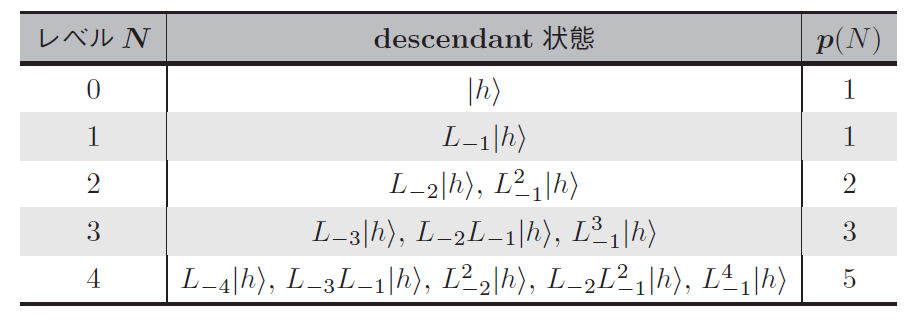
\includegraphics[width=0.6\linewidth]{fig/5.2notag.png}
\end{figure*}

$p(N) $是$ N$ 的拆分数,可通过对无穷乘积
\begin{equation}
	P(q)=\prod_{n=1}^{\infty}\left(1-q^{n}\right)
\end{equation}
\quad \quad (5.94)
的倒数作Taylor展开:
\begin{equation}
	\prod_{n=1}^{\infty}\left(1-q^{n}\right)^{-1}=\sum_{n=0}^{\infty} p(n) q^{n}, \quad|q|<1
\end{equation}
来计算。

态$ |\{n\},h\rangle$ 的Hermite共轭是
\begin{equation}
	\langle h,\{n\}|=\langle h| L_{\{n\}}=\langle h| L_{n_{k}} \cdots L_{n_{1}}
\end{equation}

为讨论Verma模 $V_h$ 中内积的正定性,有必要计算次级态间的内积$ \langle h,\{n'\}|\{n\},h\rangle $。由 $|h\rangle $的范数归一化的内积
$$
\frac{\langle h,\{n'\}|\{n\},h\rangle}{\langle h|h\rangle}
$$
称为Shapovarov形式。因为$ |\{n\},h\rangle$ 是Virasoro算符 $L_0 $的本征值为 $h+N $( $N=\sum_{i=1}^{k} n_{i}$ )的本征态,只有同级态间的内积非零。考虑级为 $N$ 的次级态间归一化内积的矩阵
\begin{equation}
	M(c, h)_{N}=\left(\frac{\left\langle h,\left\{n^{\prime}\right\} |\{n\}, h\right\rangle}{\langle h | h\rangle}\right)
\end{equation}
这是一个 $p(N)\times p(N) $矩阵。

在酉的理论中,各级Shapovarov形式都非负。正定时, $V_h$ 是Virasoro代数的不可约表示。在退化表示的情形, $V_h $中存在一个零模态。既然这时 $M(c, h)_{N} $有一个本征值为零的本征态,就可以得到Shapovarov形式非负的一个边界条件。

例如我们计算$ L_{-n}|h\rangle$ ( $n\geq 1 $)的范数,这非负的条件是
\begin{equation}
	\begin{aligned} \left\langle h\left|L_{n} L_{-n}\right| h\right\rangle &= \langle h\left|\left[L_{n}, L_{-n}\right]\right| h \rangle \\ &= \langle h |\left(2 n L_{0}+\frac{c}{12} n\left(n^{2}-1\right)\right) | h \rangle \\ &=\left(2 n h+\frac{c}{12} n\left(n^{2}-1\right)\right)\langle h |h\rangle \geq 0 \end{aligned}
\end{equation}
$n=1 $时,这是
$$
\langle h|L_1L_{-1}|h\rangle=2h\langle h|h\rangle \geq0
$$
如果 $\langle h|h\rangle>0 $,这就意味着$ h\geq 0 $。此外,考虑 $n$ 足够大的情形,如果 $c<0$ ,那么 (5.98) 是负的。因此,酉的CFT必须满足
\begin{equation}
	h \geq 0, \quad c \geq 0
\end{equation}
对前几级,$ M(c, h)_{N}$ 是
\begin{align} M(c, h)_{0} &=1\\ M(c, h)_{1} &=2 h \\ M(c, h)_{2} &=\frac{1}{\langle h | h\rangle}\left(\begin{array}{cc} \langle h,\{2\} |\{2\}, h\rangle & \langle h,\{2\} |\{1,1\}, h\rangle \\ \langle h,\{1,1\} |\{2\}, h\rangle & \langle h,\{1,1\} |\{1,1\}, h\rangle \end{array}\right) \notag\\ &=\left(\begin{array}{cc} 4 h+\frac{c}{2} & 6 h \\ 6 h & 4 h(1+2 h) \end{array}\right)  \end{align}
直接计算Shapovarov形式不容易。$ M(c, h)_{N} $的行列式称为Kac行列式\footnote{V. G. Kac, Lect. Notes. Phys. 94 (1979) 441.},$ N=0,1,2 $时是
\begin{align} &\det M(c, h)_{0}=1 \\ &\det M(c, h)_{1}=2 h \\ &\det M(c, h)_{2}=4 h\left(8 h^{2}+(c-5) h+\frac{c}{2}\right)  \end{align}
$\det M(c, h)_{N}$ 是$ h,c $的多项式。如果令$ \det M(c, h)_{N}=0 $,将得到作为 $c$ 的函数的 $h$ 。 $N=1$ 时得到$ h=0$ , $N=2 $时得到
$$
h=\frac{5-c \pm \sqrt{(c-1)(c-25)}}{16}
$$
这和 (5.30) 中 $h_{1,1},h_{1,2},h_{2,1}$ 的值是一样的。$ h$ 在Kac谱中时,Kac行列式为零。在Verma模$ V_h $中,如果有一个级为 $n(\leq N)$ 的零模态 $|h+n\rangle$ ,那么 $h,c $的值将使行列式为零。$ |h+n\rangle$ 作用上Virasoro算符得到的态
$$
L_{-n_{1}} \cdots L_{-n_{k}}|h+n\rangle, \quad n_{1} \geq \cdots \geq n_{k}\geq 1
$$
也是零模态。级为 $N $的零模态,可以要求$ n_{1}+\cdots+n_{k}=N-n $来这样构造。这些态的数目是$ p(N-n)$ 。也就是说,对应级为 $n$ 的零模态, $M(c, h)_{N} $有 $p(N-n) $个本征值为零。因为对应Kac谱中 $h_{n,m}$ 的是级为 $nm $的零模态, $\det M(c, h)_{N}$ 包含因子 $\left(h-h_{n, m}\right)^{p(N-n m)} $。Kac猜想
\begin{equation}
	\operatorname{det} M(c, h)_{N}=\alpha_{N} \prod_{n m \leq N}\left(h-h_{n, m}\right)^{p(N-n m)}
\end{equation} 
$\alpha_N$ 是一正常数。这个猜想后来被Feigin-Fuchs\footnote{B. L. Feigin and D. B. Fuchs, Funct. Anal. and Appl. 16 (1984) 114, 17 (1983) 241.}证明了。这里令 $\alpha_{-}=\sqrt{\frac{q}{q+1}}$ 将很方便,那么中心荷是
\begin{equation}
	c=1-\frac{6}{q(q+1)}
\end{equation}
取逆得到
\begin{equation}
	q=-\frac{1 \pm \sqrt{\frac{25-c}{1-c}}}{2}
\end{equation}
Kac谱中的 $h_{n,m}$可写成
\begin{equation}
	h_{n, m}=\frac{[(q+1) n-q m]^{2}-1}{4 q(q+1)}
\end{equation}

Kac行列式可能在 $(c,h) $空间中的一处区域内是正的,另一处则是负的。在负的区域, $M(c, h)_{N}$ 有奇数个负本征值,内积不正定。在各级排除掉行列式是负的情形,或者找到一个关于$ c,h $的条件使得行列式非负,就是CFT酉的必要条件。首先,考虑$ c\geq1,h\geq 0 $的情形,如果 $1<c<25$ ,那么$q $有虚部,因而$ h_{n,m} $有虚部( $n\neq m $)或是负的($ n=m $)。所以, $h>0$ 时,$ \det M(c, h)_{N}$ 不会为零。另一方面,$ h$ 很大时,$\det M(c, h)_{N} $是正的,因此 $h>0$ 时行列式总是正的。

如果 $c\geq 25$ ,那么 $-1<q<0$ 。这时 $h_{n,m} $是负的,$ h>0$ 时 $\det M(c, h)_{N}$是正的。如果$ c=1$ ,那么$ h_{n, m}=\frac{(n-m)^{2}}{4}$ ,$ h\geq 0 $时$ \det M(c, h)_{N} $有零点,但总不会是负的。因此,如果 $c\geq1,h\geq 0$ ,从行列式的讨论中得不出理论非酉。

\begin{figure}[h]
	\centering
	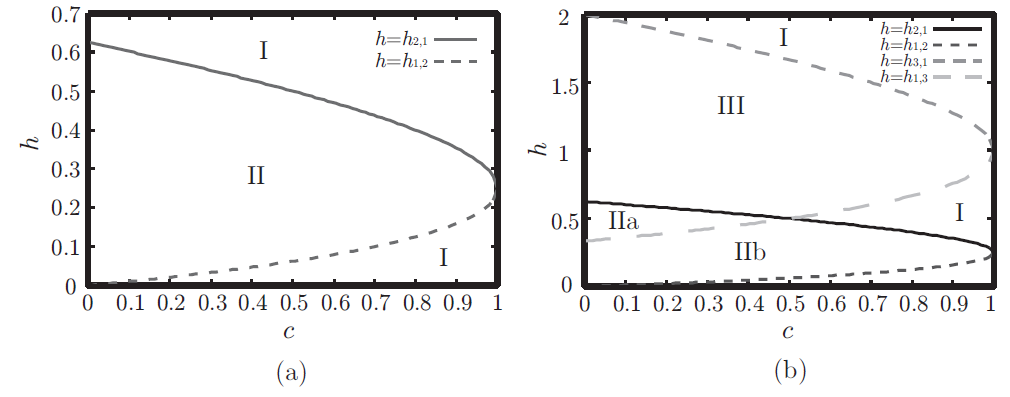
\includegraphics[width=0.7\linewidth]{fig/5.2.png}
	\caption{$(c,h)$平面上的酉区域。(a)级$N=2$,(b)$N=3$。}
\end{figure}

$0<c<1 $时,$Kac$行列式的正负区域由曲线 $h=h_{n, m}(c)$ 分开。这条曲线在 $c=0 $时的值是 $h=\frac{(3 n-2 m)^{2}-1}{24} $, $c=1$ 时的值是 $h=\frac{(n-m)^{2}}{4} $。我们在各级排除掉行列式是负的情形。 $N=1$ 时,这给出$ h\geq 0 $。 $N=2 $时,在图5.2(a)的 $h=h_{2,1}(c) $和 $h=h_{1,2}(c)$ 围起来的区域II中, $\det M(c, h)_{2}<0$ 。在边界上理论可能是酉的。

然后考虑$ N=3 $的情形。可以看到,在图5.2(b)的区域III和IIb中, $\det M(c, h)_{3}<0 $。 $N=2 $时已经排除了区域IIa,那么区域IIa,IIb和III就都被排除了。在边界$ h=h_{1,3} $上,位于区域II中的部分也被排除了。同理,在边界 $h=h_{2,1} $上,区域IIa和III间的线段也被排除了。剩下 $h=h_{2,1}$ 和 $h=h_{1,3}$ 的交点$ (c,h)=(1/2,1/2) $。讨论更高级时不会排除掉这个点,它刚好对应Ising模型。重复这些论证将得到,酉的理论对应$ q=3,4,5,\cdots$ 。这点是由Friedan-Qiu-Shenker\footnote{D. Friedan, Z. a. Qiu and S. H. Shenker, Phys. Rev. Lett. 52 (1984) 1575.}\footnote{D. Friedan, S. H. Shenker and Z. a. Qiu, Commun. Math. Phys. 107 (1986) 535.}\footnote{D. Friedan, Z. a. Qiu and S. H. Shenker, “Conformal Invariance, Unitarity and Two Dimensional Critical Exponents” in Vertex Operators in Mathematical Physics, Springer–Verlag, 1984.}证明的。Goddard-Kent-Olive\footnote{P. Goddard, A. Kent and D. I. Olive, Commun. Math. Phys. 103 (1986) 105.}证明了,这不只是酉的必要条件,也是充分条件。

\section{共形块和单值变换不变性}
4.4节讨论过,四点关联函数具有交叉对称性。本节,我们调查含极小模型中退化初级场的四点关联函数的全局性质。在5.2节,我们推导了含退化初级场的关联函数满足的微分方程,并将含场 $\phi_{(1,2)}$ 的四点关联函数写成超几何级数。考虑到反全纯部分,四点函数$ G_{32}^{10}(x, \bar{x})=\left\langle\phi_{(2,1)}(\infty, \infty) \phi_{1}(1,1) \phi_{2}(x, \bar{x}) \phi_{3}(0,0)\right\rangle$ 是
\begin{equation}
	G_{32}^{10}(x, \bar{x})=|x|^{2 a_{1}+2 a_{2}}|1-x|^{2 b_{1}+2 b_{2}} \sum_{i, j=1}^{2} X_{i j} y_{i}^{(0)}(x) \overline{y_{j}^{(0)}(x)} 
\end{equation}
其中 $a_{1}+a_{2}=h\left(\alpha_{1}-\alpha_{-}\right)-h_{2}-h_{3} $, $b_{1}+b_{2}=h\left(\alpha_{3}-\alpha_{-}\right)-h_{1}-h_{2}$ , $X_{ij}$ 是常数, $y_{1}^{(0)}(x), y_{2}^{(0)}(x) $是超几何微分方程 (5.41) 在$ x=0$ 附近的基本解 (5.46),(5.48) 。这个关联函数的表达式是在 $x=0$ 附近得到的,但关联函数本身定义在除去$ x=0,1,\infty $的复平面上。它的值在给定 $x $处应当是唯一确定的。另一方面,这个微分方程的解有固定奇点$ x=0,1,\infty $,沿绕奇点的路径延拓时会经历带相位因子的变换。解的这个变换称为单值变换。由于物理的要求,关联函数的值在给定 $x$ 处唯一确定, $G_{32}^{10}(x, \bar{x}) $应当在单值变换下不变。

\begin{figure}[h]
	\centering
	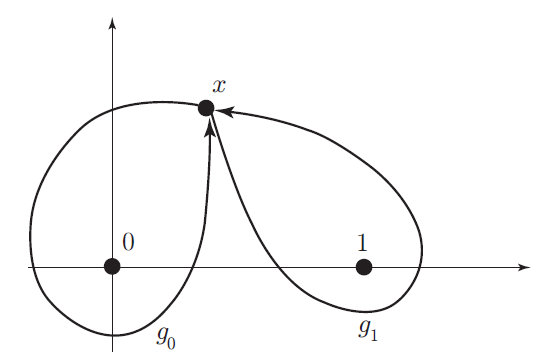
\includegraphics[width=0.6\linewidth]{fig/5.3.png}
	\caption{绕$x=0,1$时经历的单值变换。}
\end{figure}

从点 $x$ 出发,逆时针沿绕 $x=0 $的闭合曲线时经历的变换记作 $g_0$ ,绕 $x=1$ 的记作 $g_1$ ,如图5.3。因为绕无穷远点的 $g_\infty $由$ g_1g_0 $生成,验证 $g_0,g_1 $下不变就足够了。

绕$ x=0$ 一圈,也就是 $x \rightarrow x e^{2 \pi i} $, $y_{1}^{(0)}(x), y_{2}^{(0)}(x) $变换为
\begin{equation}
	g_{0}\left(\begin{array}{c} y_{1}^{(0)}(x) \\ y_{2}^{(0)}(x) \end{array}\right)=\left(\begin{array}{cc} 1 & 0 \\ 0 & \omega_{0} \end{array}\right)\left(\begin{array}{l} y_{1}^{(0)}(x) \\ y_{2}^{(0)}(x) \end{array}\right)
\end{equation} 
其中 $\omega_{0}=\exp (2 \pi i(1-\gamma)) $。$ G_{32}^{10}(x, \bar{x})$ 在变换 $g_0 $下不变,要求$ X_{i j}$ 满足
$$
\sum_{i, j} X_{i j}\left(g_{0}\right)_{i k} \overline{\left(g_{0}\right)}_{j l}=X_{k l}
$$
因为$ \left(g_{0}\right)_{i k} $是对角矩阵 $\left(g_{0}\right)_{i i} \delta_{i k}$ ,上式即
$$
		X_{k l}\left(g_{0}\right)_{k k} \overline{\left(g_{0}\right)}_{l l}=X_{k l} 
$$
那么 $i\neq j $时 $X_{ij}=0 $。因此四点函数可写成
\begin{equation}
	G_{32}^{10}(x, \bar{x})=|x|^{2 a_{1}+2 a_{2}}|1-x|^{2 b_{1}+2 b_{2}} \sum_{i=1}^{2} X_{i i} y_{i}^{(0)}(x) \overline{y_{i}^{(0)}(x)} 
\end{equation}
考虑 $x=1$ 附近的单值变换。令 $\xi=1-x $, (5.41) 成为
\begin{equation}
	\xi(1-\xi) \frac{d^{2} y}{d \xi^{2}}+(\alpha+\beta+1-\gamma-(\alpha+\beta+1) \xi) \frac{d y}{d \xi}-\alpha \beta y=0
\end{equation} 
那么这时的级数解 $y_{1}^{(1)}(x), y_{2}^{(1)}(x) $相比$ x=0 $附近的,要将 $\alpha,\beta,\gamma$ 换成 $\alpha,\beta,\alpha+\beta+1-\gamma $:
\begin{equation}
	\begin{aligned} &y_{1}^{(1)}(x)=F(\alpha, \beta, 1+\alpha+\beta-\gamma, 1-x) \\ &y_{2}^{(1)}(x)=(1-x)^{\gamma-\alpha-\beta} F(\gamma-\beta, \gamma-\alpha, 1+\gamma-\alpha-\beta, 1-x) \end{aligned}
\end{equation}
对这个解,绕 $x=1$ 一圈,也就是 $1-x \rightarrow(1-x) e^{2 \pi i} $, $y_{1}^{(1)}(x), y_{2}^{(1)}(x)$ 变换为
\begin{equation}
	g_{1}\left(\begin{array}{c} y_{1}^{(1)}(x) \\ y_{2}^{(1)}(x) \end{array}\right)=\left(\begin{array}{cc} 1 & 0 \\ 0 & \omega_{1} \end{array}\right)\left(\begin{array}{l} y_{1}^{(1)}(x) \\ y_{2}^{(1)}(x) \end{array}\right)
\end{equation} 
其中 $\omega_{1}=\exp (2 \pi i(\gamma-\alpha-\beta))$ 。

对无穷远点 $x=\infty $也类似。令$ x=1/\xi$ , $y=\xi^{\alpha} y^{\prime} $, (5.41) 成为
\begin{equation}
	\xi(1-\xi) \frac{d^{2} y^{\prime}}{d \xi^{2}}+(\alpha-\beta+1-(2 \alpha-\gamma+2) \xi) \frac{d y^{\prime}}{d \xi}-\alpha(\alpha-\gamma+1) y^{\prime}=0
\end{equation} 
那么这时的级数解$ y_{1}^{(\infty)}(x), y_{2}^{(\infty)}(x) $相比$ x=0$ 附近的,要将$ \alpha,\beta,\gamma$ 换成 $\alpha,\alpha-\gamma+1,\alpha-\beta+1$ :
\begin{equation}
	\begin{aligned} &y_{1}^{(\infty)}(x)=x^{-\alpha} F\left(\alpha, \alpha+1-\gamma, \alpha+1-\beta, \frac{1}{x}\right) \\ &y_{2}^{(\infty)}(x)=x^{-\beta} F\left(\beta, \beta+1-\gamma, \beta+1-\alpha, \frac{1}{x}\right) \end{aligned}
\end{equation}
单值变换是
\begin{equation}
	g_{\infty}\left(\begin{array}{c} y_{1}^{(\infty)}(x) \\ y_{2}^{(\infty)}(x) \end{array}\right)=\left(\begin{array}{cc} e^{-2 \pi i \alpha} & 0 \\ 0 & e^{-2 \pi i \beta} \end{array}\right)\left(\begin{array}{l} y_{1}^{(\infty)}(x) \\ y_{2}^{(\infty)}(x) \end{array}\right)
\end{equation} 
这三点附近的基本解间有关系
\begin{align} &y_{i}^{(0)}(x)=\sum_{j=1}^{2} a_{i j} y_{j}^{(1)}(x \\ &y_{i}^{(0)}(x)=\sum_{j=1}^{2} b_{i j} y_{j}^{(\infty)}(x) \end{align}
借助超几何级数的解析延拓公式\footnote{犬井鉄郎,『特殊函数』,岩波全書,1962.}
\begin{align} F(\alpha, \beta, \gamma, x)=& \frac{\Gamma(\gamma) \Gamma(\gamma-\alpha-\beta)}{\Gamma(\gamma-\alpha) \Gamma(\gamma-\beta)} F(\alpha, \beta, 1+\alpha+\beta-\gamma, 1-x) \notag\\ &+\frac{\Gamma(\gamma) \Gamma(\alpha+\beta-\gamma)}{\Gamma(\alpha) \Gamma(\beta)}(1-x)^{\gamma-\alpha-\beta} \\ & \times F(\gamma-\beta, \gamma-\alpha, 1+\gamma-\alpha-\beta, 1-x)\notag\\ F(\alpha, \beta, \gamma, x)=& \frac{\Gamma(\gamma) \Gamma(\beta-\alpha)}{\Gamma(\beta) \Gamma(\gamma-\alpha)}(-x)^{-\alpha} F\left(\alpha, 1+\alpha-\gamma, 1+\alpha-\beta, \frac{1}{x}\right) \notag\\ &+\frac{\Gamma(\gamma) \Gamma(\alpha-\beta)}{\Gamma(\alpha) \Gamma(\gamma-\beta)}(-x)^{-\beta} F\left(\beta, 1+\beta-\gamma, 1+\beta-\alpha, \frac{1}{x}\right) \end{align}
我们得到变换矩阵$ a_{ij},b_{ij} $是
\begin{align} &\left(a_{i j}\right)=\left(\begin{array}{cc} \frac{\Gamma(\gamma) \Gamma(\gamma-\alpha-\beta)}{\Gamma(\gamma-\alpha) \Gamma(\gamma-\beta)} & \frac{\Gamma(\gamma) \Gamma(\alpha+\beta-\gamma)}{\Gamma(\alpha) \Gamma(\beta)} \\ \frac{\Gamma(2-\gamma) \Gamma(\gamma-\alpha-\beta)}{\Gamma(1-\alpha) \Gamma(1-\beta)} & \frac{\Gamma(2-\gamma) \Gamma(\alpha+\beta-\gamma)}{\Gamma(\alpha-\gamma+1) \Gamma(\beta-\gamma+1)} \end{array}\right) \\ &\left(b_{i j}\right)=\left(\begin{array}{cc} \frac{\Gamma(\gamma) \Gamma(\beta-\alpha)}{\Gamma(\beta) \Gamma(\gamma-\alpha)} e^{-\pi i \alpha} & \frac{\Gamma(\gamma) \Gamma(\alpha-\beta)}{\Gamma(\alpha) \Gamma(\gamma-\beta)} e^{-\pi i \beta} \\ \frac{\Gamma(2-\gamma) \Gamma(\beta-\alpha)}{\Gamma(\beta-\gamma+1) \Gamma(1-\alpha)} e^{-\pi i(\alpha-\gamma+1)} &\frac{\Gamma(2-\gamma) \Gamma(\alpha-\beta)}{\Gamma(\alpha-\gamma+1) \Gamma(1-\beta)} e^{-\pi i(\beta-\gamma+1)} \end{array}\right)\end{align}
(5.119) 代入 (5.112) ,得到$ G_{32}^{10}(x, \bar{x})$ 在$ x=1$ 附近的级数表示:
\begin{align} &G_{32}^{10}(x, \bar{x})=|x|^{2 a_{1}+2 a_{2}}|1-x|^{2 b_{1}+2 b_{2}} \sum_{i, j=1}^{2} X_{i j}^{1} y_{i}^{(1)}(x) \overline{y_{j}^{(1)}(x)} \\ &X_{i j}^{1}=\sum_{k=1}^{2} X_{k k} a_{k i} \bar{a}_{k j} \end{align}

关联函数在 $g_1 $下不变,要求$ X_{i j}^{1} $的非对角项$ X_{12}^{1} $为零,那么
$$
X_{11} a_{11} \bar{a}_{12}+X_{22} a_{21} \bar{a}_{22}=0
$$
换言之
\begin{equation}
	\begin{aligned} \frac{X_{11}}{X_{22}} &=-\frac{a_{21} \bar{a}_{22}}{a_{11} \bar{a}_{12}} \\ &=-\frac{\Gamma(2-\gamma)^{2} \Gamma(\alpha) \Gamma(\beta) \Gamma(\gamma-\alpha) \Gamma(\gamma-\beta)}{\Gamma(\gamma)^{2} \Gamma(1-\alpha) \Gamma(1-\beta) \Gamma(\alpha-\gamma+1) \Gamma(\beta-\gamma+1)} \end{aligned}
\end{equation} 
因此四点函数可写成
\begin{equation}
	\begin{aligned} G_{32}^{10}(x, \bar{x})=&|x|^{2 h\left(\alpha_{1}-\alpha_{-}\right)-2 h_{2}-2 h_{3}}|1-x|^{2 h\left(\alpha_{3}-\alpha_{-}\right)-2 h_{1}-2 h_{2}} \\ & \times \lambda\left(\frac{\Gamma(\alpha) \Gamma(\beta) \Gamma(\gamma-\alpha) \Gamma(\gamma-\beta)}{\Gamma(\gamma)^{2}}\left|y_{1}^{(0)}(x)\right|^{2}\right.\\&\left.-\frac{\Gamma(1-\alpha) \Gamma(1-\beta) \Gamma(1-\gamma+\alpha) \Gamma(1-\gamma+\beta)}{\Gamma(2-\gamma)^{2}}\left|y_{2}^{(0)}(x)\right|^{2}\right) \end{aligned}
\end{equation} 
其中 $\lambda$ 是常数。$ G_{32}^{10}(x, \bar{x}) $在 $x=1 $附近可写成
\begin{equation}
	\begin{aligned} G_{32}^{10}(x, \bar{x})=&|x|^{2 h\left(\alpha_{1}-\alpha_{-}\right)-2 h_{2}-2 h_{3}}|1-x|^{2 h\left(\alpha_{3}-\alpha_{-}\right)-2 h_{1}-2 h_{2}} \\ & \times \lambda^{\prime}\left(\frac{\Gamma(\gamma-\alpha-\beta)^{2}}{\Gamma(1-\alpha) \Gamma(1-\beta) \Gamma(\gamma-\alpha) \Gamma(\gamma-\beta)}\left|y_{1}^{(1)}(x)\right|^{2}\right.\\&\left.-\frac{\Gamma(\alpha+\beta-\gamma)^{2}}{\Gamma(\alpha) \Gamma(\beta) \Gamma(1+\alpha-\gamma) \Gamma(1+\beta-\gamma)}\left|y_{2}^{(1)}(x)\right|^{2}\right) \end{aligned}
\end{equation} 
其中
\begin{equation}
	\begin{aligned} \lambda^{\prime}=& \lambda \frac{\Gamma(\alpha) \Gamma(1-\alpha) \Gamma(\beta) \Gamma(1-\beta)}{\Gamma(\gamma) \Gamma(1-\gamma)} \\ & \times \frac{\Gamma(\gamma-\alpha) \Gamma(1+\alpha-\gamma) \Gamma(\gamma-\beta) \Gamma(1+\beta-\gamma)}{\Gamma(\gamma-\alpha-\beta) \Gamma(1+\alpha+\beta-\gamma)} \end{aligned} 
\end{equation}

计算关联函数的具体例子,有描述Ising模型\footnote{A. A. Belavin, A. M. Polyakov and A. B. Zamolodchikov, Nucl. Phys. B 241 (1984) 333.}和Yang-Lee边界奇点\footnote{J. L. Cardy, Phys. Rev. Lett. 54 (1985) 1345.}的极小模型。Yang-Lee边界奇点对应CFT的中心荷是 $c=-22/5$ ,含恒等算符$ \boldsymbol{I}$ 和共形权是$ (-1/5,-1/5)$ 的初级场$ \varphi=\phi_{(1,2)}$ 。这个模型中非平凡的四点函数是
$$
\left\langle\varphi\left(z_{1}, \bar{z}_{1}\right) \varphi\left(z_{2}, \bar{z}_{2}\right) \varphi\left(z_{3}, \bar{z}_{3}\right) \varphi\left(z_{4}, \bar{z}_{4}\right)\right\rangle
$$
这时 $t=2/5 $, $\alpha_{1}=\alpha_{2}=\alpha_{3}=\alpha_{+}+2 \alpha_{-}$ ,我们有
\begin{align} &a_1=b_1=0,\quad a_2=b_2=2/5\\ &\alpha=4/5,\quad \beta=3/5,\quad \gamma=6/5 \end{align}
因此
\begin{equation}
	\begin{aligned} G_{\varphi \varphi}^{\varphi \varphi}(x, \bar{x})=\lambda|x|^{\frac{4}{5}}|1-x|^{\frac{4}{5}} &\left\{N_{1}\left|F\left(\frac{4}{5}, \frac{3}{5}, \frac{6}{5}, x\right)\right|^{2}\right.\\&\left.+N_{2}\left|x^{-\frac{1}{5}} F\left(\frac{3}{5}, \frac{2}{5}, \frac{4}{5}, x\right)\right|^{2}\right\} \end{aligned} 
\end{equation}
其中
\begin{align} &N_{1}=\frac{\Gamma\left(4/5\right) \Gamma\left(3/5\right)^{2} \Gamma\left(2/5\right)}{\Gamma\left(6/5\right)} \\ &N_{2}=-\frac{\Gamma\left(1/5\right) \Gamma\left(2/5\right)^{2} \Gamma\left(3/5\right)}{\Gamma\left(4/5\right)^{2}} \end{align}

接着考虑Ising模型,它含恒等算符 $\boldsymbol{I}$ ( $h=\bar{h}=0 $),自旋算符$ \sigma(z, \bar{z})=\phi_{(1,2)}(z, \bar{z})$ ( $h=\bar{h}=1/16$ )和能量密度算符 $\epsilon(z, \bar{z})=\phi_{(2,1)}(z, \bar{z}) $( $h=\bar{h}=1/2 $)。考虑自旋算符的四点函数
$$
\left\langle\sigma\left(z_{0}, \bar{z}_{0}\right) \sigma\left(z_{1}, \bar{z}_{1}\right) \sigma\left(z_{2}, \bar{z}_{2}\right) \sigma\left(z_{3}, \bar{z}_{3}\right)\right\rangle
$$
这时 $h_{0}=h_{1}=h_{2}=h_{3} =1/16 $,我们有
\begin{equation}
	\begin{aligned} &a_{1}=b_{1}=0, \quad a_{2}=b_{2}=-1/8 \\ &\alpha=-1/4,\quad \beta=1/4,\quad \gamma=1/2
	 \end{aligned}
\end{equation}
于是关联函数可写成
\begin{equation}
	\left\langle\sigma\left(z_{0}, \bar{z}_{0}\right) \sigma\left(z_{1}, \bar{z}_{1}\right) \sigma\left(z_{2}, \bar{z}_{2}\right) \sigma\left(z_{3}, \bar{z}_{3}\right)\right\rangle=\left|\frac{z_{13} z_{02}}{z_{01} z_{23} z_{12} z_{03}}\right|^{\frac{1}{4}} F(x, \bar{x})
\end{equation}
$F(x, \bar{x}) $满足微分方程
\begin{equation}
	x(1-x) \frac{d^{2} F}{d x^{2}}+\left(\frac{1}{2}-x\right) \frac{d F}{d x}+\frac{1}{16} F=0
\end{equation}
令$ x=\sin^2\theta $,这成为
$$
\left(\frac{d^{2}}{d \theta^{2}}+\frac{1}{4}\right) F=0
$$
解得
\begin{equation}
	F_{1}=\cos \frac{\theta}{2}=\frac{1}{2} \sqrt{1+\sqrt{1-x}}, \quad F_{2}=\sin \frac{\theta}{2}=\frac{1}{2} \sqrt{1-\sqrt{1-x}}
\end{equation}
$F(x, \bar{x})$ 可写成$ F_i,\bar{F}_j $的组合:
\begin{equation}
	F(x, \bar{x})=u_{11} F_{1} \bar{F}_{1}+u_{22} F_{2} \bar{F}_{2}+u_{12} F_{1} \bar{F}_{2}+u_{21} F_{2} \bar{F}_{1}
\end{equation} 
绕$ x=0,1,\infty $一圈经历的单值变换是
\begin{align} &F_{1} \rightarrow F_{1}, \quad F_{2} \rightarrow e^{\pi i} F_{2}, \quad x=0\quad \\ &F_{1} \rightarrow F_{2}, \quad F_{2} \rightarrow F_{1}, \quad x=1\quad\\ &F_{1} \rightarrow e^{-\pi i} F_{1}, \quad F_{2} \rightarrow e^{-\pi i} F_{2}, \quad x=\infty\quad  \end{align}
不变性要求 $u_{11}=u_{22} $, $u_{12}=u_{21}=0$ ,因此有
\begin{equation}
	\begin{aligned} F(x, \bar{x})=\lambda\left( \sqrt{1+\sqrt{1-x}} \sqrt{1+\sqrt{1-\bar{x}}}+\sqrt{1-\sqrt{1-x}} \sqrt{1-\sqrt{1-\bar{x}}}\right) \end{aligned}
\end{equation}

\section{四点函数和OPE系数}
上节展示了,含退化初级场$ \phi_{(1,2)}$ 的四点关联函数可写成超几何级数。本节,我们从退化初级场的四点函数
\begin{equation}
	\left\langle\phi_{(1,2)}(\infty, \infty) \phi_{\left(n_{1}, m_{1}\right)}(1,1) \phi_{\left(n_{2}, m_{2}\right)}(x, \bar{x}) \phi_{\left(n_{3}, m_{3}\right)}(0,0)\right\rangle 
\end{equation}
中,提取有关退化初级场OPE系数的信息。

(5.145) 中令$ x $趋于零,用OPE
\begin{equation}
\begin{aligned} \phi_{\left(n_{2}, m_{2}\right)}(x, \bar{x}) \phi_{\left(n_{3}, m_{3}\right)}(0,0)=& \sum_{(n, m)} C_{\left(n_{2}, m_{2}\right)\left(n_{3}, m_{3}\right)}^{(n, m)}|x|^{2 h_{n, m}-2 h_{n_{2},m_2}-2 h_{n_{3},m_3}} \\ & \times\left(\phi_{(n, m)}(0,0)+\cdots\right) \end{aligned}
\end{equation} 
将关联函数展开成
\begin{equation}
	\begin{aligned} &\sum_{(n, m)} C_{\left(n_{2}, m_{2}\right)\left(n_{3}, m_{3}\right)}^{(n, m)}|x|^{2 h_{n,m}-2 h_{n_{2}, m_{2}}-2 h_{n_{3}, m_{3}}} \\ &\times\left\langle\phi_{(1,2)}(\infty, \infty) \phi_{\left(n_{1}, m_{1}\right)}(1,1) \phi_{(n, m)}(0,0)\right\rangle+\cdots \end{aligned}
\end{equation} 
两点和三点函数的归一化条件选为
\begin{align} &\left\langle\phi_{(n_1, m_1)}\left(z_{1}, \bar{z}_{1}\right) \phi_{\left(n_2, m_2\right)}\left(z_{2}, \bar{z}_{2}\right)\right\rangle=\delta_{n_{1}, n_{2}} \delta_{m_{1}, m_{2}}\left|z_{12}\right|^{-4 h_{n_{1},m_1}}\\ &\left\langle\phi_{\left(n_{1}, m_{1}\right)}\left(z_{1}, \bar{z}_{1}\right) \phi_{\left(n_{2}, m_{2}\right)}\left(z_{2}, \bar{z}_{2}\right) \phi_{\left(n_{3}, m_{3}\right)}\left(z_{3}, \bar{z}_{3}\right)\right\rangle \notag\\ &=C_{\left(n_{1}, m_{1}\right)\left(n_{2}, m_{2}\right)\left(n_{3}, m_{3}\right)}\left|z_{12}\right|^{2 h_{3}-2 h_{1}-2 h_{2}}\left|z_{23}\right|^{2 h_{1}-2 h_{2}-2 h_{3}}\left|z_{13}\right|^{2 h_{2}-2 h_{1}-2 h_{3}} 
\end{align}
其中$ h_{i}=h_{n_{i}, m_{i}}$ ( $i=1,2,3 $)。 $C_{\left(n_{1}, m_{1}\right)\left(n_{2}, m_{2}\right)\left(n_{3}, m_{3}\right)} $关于 $(n_i,m_i) $是对称的。取$ \phi_{\left(n_{1}, m_{1}\right)}$ 和 $\phi_{\left(n_{2}, m_{2}\right)} $的OPE,并用两点函数的归一化条件,可以得到 $C_{\left(n_{1}, m_{1}\right)\left(n_{2}, m_{2}\right)\left(n_{3}, m_{3}\right)}=C_{\left(n_{1}, m_{1}\right)\left(n_{2}, m_{2}\right)}^{\left(n_{3}, m_{3}\right)} $。注意,如果含恒等算符 $\phi_{(1,1)}$ ,那么 (5.148) 给出 $C_{\left(n_{2}, m_{2}\right)\left(n_{3}, m_{3}\right)}^{(1,1)}=\delta_{n_{2}, n_{3}} \delta_{m_{2}, m_{3}}$ 。
特别地,三点$ (z_1,z_2,z_3)$ 选成$ (\infty, 1,0) $,使用同 (4.65) 一样的定义,可以得到 (5.147) 中的三点函数就是OPE系数本身:
\begin{equation}
\left\langle\phi_{(1,2)}(\infty, \infty) \phi_{\left(n_{1}, m_{1}\right)}(1,1) \phi_{(n, m)}(0,0)\right\rangle=C_{(1,2)\left(n_{1}, m_{1}\right)(n, m)}
\end{equation} 
根据融合规则,它的值仅当$ (n, m)=\left(n_{1}, m_{1} \pm 1\right) $时非零。因此 (5.147) 等于
\begin{equation}
	\sum_{l=\pm 1} C_{\left(n_{2}, m_{2}\right)\left(n_{3}, m_{3}\right)}^{\left(n_{1}, m_{1}+l\right)} C_{(1,2)\left(n_{1}, m_{1}\right)}^{\left(n_{1}, m_{1}+l\right)}|x|^{2 h_{n_1, m_1+l}-2 h_{n_{2}, m_{2}}-2 h_{n_{3}, m_{3}}}
\end{equation}
与关联函数的超几何级数表达式 (5.128) 比对。在 (5.151) 中,$ l=-1 $项对应 (5.128) 第一项,$ l=+1 $项则对应第二项,于是得到
\begin{align} C_{\left(n_{2}, m_{2}\right)\left(n_{3}, m_{3}\right)}^{\left(n_{1}, m_{1}-1\right)} C_{(1,2)\left(n_{1}, m_{1}\right)}^{\left(n_{1}, m_{1}-1\right)}=& \lambda \frac{\Gamma(\alpha) \Gamma(\beta) \Gamma(\gamma-\alpha) \Gamma(\gamma-\beta)}{\Gamma(\gamma)^{2}} \\ C_{\left(n_{2}, m_{2}\right)\left(n_{3}, m_{3}\right)}^{\left(n_{1}, m_{1}+1\right)} C_{(1,2)\left(n_{1}, m_{1}\right)}^{\left(n_{1}, m_{1}+1\right)}=&-\lambda \Gamma(1-\alpha) \Gamma(1-\beta) \notag\\ & \times \frac{\Gamma(1-\gamma+\alpha) \Gamma(1-\gamma+\beta)}{\Gamma(2-\gamma)^{2}} \end{align}
其中
\begin{align} &\alpha=\frac{1}{2}\left(1+n_{1}+n_{2}+n_{3}-t\left(m_{1}+m_{2}+m_{3}\right)\right)\\ &\beta=\frac{1}{2}\left(1+n_{1}-n_{2}+n_{3}-t\left(m_{1}-m_{2}+m_{3}\right)\right)\\ &\gamma=1+n_{1}-m_{1} t \end{align}

例如,考虑初级场都是 $\phi_{(1,2)}$ ,即 $\left(n_{i}, m_{i}\right)=(1,2) $的情形。归一化给出$ C_{(1,2)(1,2)}^{(1,1)}=1$ ,代入 (5.152) 可求出$ \lambda$ ,于是由 (5.153) 得到
\begin{equation}
	\begin{aligned} C_{(1,2)(1,2)}^{(1,3)} &=\frac{\Gamma(2-2 t)}{\Gamma(2 t)}(-\gamma(t) \gamma(-1+3 t))^{\frac{1}{2}} \\ &=\frac{\Gamma(2-2 t)}{\Gamma(2 t)}\left(-\frac{\gamma(t)^{3}}{\gamma(3 t-1)}\right)^{\frac{1}{2}} \frac{\gamma(1-t)}{\gamma(2-3 t)} \end{aligned} 
\end{equation}
这里, $C_{(1,2)(1,2)}^{(1,3)} $选取正的,
\begin{equation}
	\gamma(x)=\frac{\Gamma(x)}{\Gamma(1-x)}
\end{equation}
$\gamma(x) $满足 $\gamma(x) \gamma(1-x)=1 $。

接着考虑 $\left(n_{1}, m_{1}\right)=(1,2) $, $\left(n_{2}, m_{2}\right)=\left(n_{3}, m_{3}\right)=(n, m) $的情形,这时四点函数是
\begin{equation}
	\left\langle\phi_{(1,2)}(\infty, \infty) \phi_{(1,2)}(1,1) \phi_{(n, m)}(x, \bar{x}) \phi_{(n, m)}(0,0)\right\rangle
\end{equation}
$\alpha=1+n-t(m+1)$, $\beta=1-t$ , $\gamma=2-2 t $。归一化给出 (5.152) 左边是 1 ,那么
\begin{equation}
\lambda=\frac{\Gamma(2-2 t)^{2}}{\Gamma(1+n-t(m+1)) \Gamma(1-n-t(1-m)) \Gamma(1-t)^2}
\end{equation}
(5.153) 左边是$ C_{(n, m)(n, m)}^{(1,3)} C_{(1,2)(1,2)}^{(1,3)} $,代入 (5.157) 得到
\begin{equation}
	C_{(n, m)(n, m)}^{(1,3)}=\frac{\Gamma(2-2 t)}{\Gamma(2 t)}\left(-\frac{\gamma(t)^{3}}{\gamma(3 t-1)}\right)^{\frac{1}{2}} \frac{\gamma(-n+t(m+1))}{\gamma(1+n-t(m+1))}
\end{equation}

考虑四点函数 (5.159) 在 $x\to 1$ 时的极限,我们得到OPE系数间的另一条关系。这时取 $\phi_{(1,2)}(1,1) 和 \phi_{(n, m)}(x, \bar{x}) $的OPE, (5.159) 等于
\begin{equation}
	\sum_{l=\pm 1} C_{(1,2)(n, m)}^{(n, m+l)} C_{(1,2)(n, m)}^{(n, m+l)}|x-1|^{2 h_{n, m+l}-2 h_{1,2}-2 h_{n, m}}+\cdots 
\end{equation}
与 (5.129) 比对得到
\begin{align} &C_{(1,2)(n, m)}^{(n, m-1)} C_{(1,2)(n, m)}^{(n, m-1)}=\lambda^{\prime} \frac{\Gamma(\gamma-\alpha-\beta)^{2}}{\Gamma(1-\alpha) \Gamma(1-\beta) \Gamma(\gamma-\alpha) \Gamma(\gamma-\beta)}\\ &C_{(1,2)(n, m)}^{(n, m+1)} C_{(1,2)(n, m)}^{(n, m+1)}=-\lambda^{\prime} \frac{\Gamma(\alpha+\beta-\gamma)^{2}}{\Gamma(\alpha) \Gamma(\beta) \Gamma(1+\alpha-\gamma) \Gamma(1+\beta-\gamma)} \end{align}
代入 $\alpha,\beta,\gamma $的值得到OPE系数
\begin{align} &C_{(1,2)(n, m)}^{(n, m-1)}=\left(\frac{\gamma(2-2 t) \gamma(-n+t m))}{\gamma(1-t) \gamma(1-n+t(m-1))}\right)^{\frac{1}{2}} \\ &C_{(1,2)(n, m)}^{(n, m+1)}=\left(\frac{\gamma(2-2 t) \gamma(n-t m))}{\gamma(1-t) \gamma(1+n+t(m+1))}\right)^{\frac{1}{2}} \end{align}

例如,在Yang-Lee边界奇点的情形,$ t=2/5$ , $\varphi=\phi_{(1,2)}=\phi_{(1,3)}$ 间的OPE系数 (5.157) 是
\begin{equation}
	C_{\varphi \varphi}^{\varphi}=\frac{i}{5} \frac{\Gamma\left(1/5\right)^2}{\Gamma\left(4/5\right) \Gamma\left(3/5\right)}\left(\frac{\sqrt{5}-1}{2}\right)^{\frac{1}{2}}
\end{equation}
那么OPE是
\begin{equation}
	\varphi(z, \bar{z}) \varphi(0,0)=C_{\varphi \varphi}^{\varphi}|z|^{\frac{2}{5}} \varphi(0,0)+\cdots
\end{equation}
$C_{\varphi \varphi}^{\varphi} $是纯虚数,说明CFT非酉。

在Ising模型的情形,$ \sigma=\phi_{(1,2)}$ , $\epsilon=\phi_{(1,3)} $, $t=3/4$ , (5.157) 是
\begin{equation}
	C_{\sigma \sigma}^{\epsilon}=\frac{1}{2}
\end{equation} 
那么$ \sigma(z, \bar{z})$ 间的OPE是
\begin{equation}
	\sigma(z, \bar{z}) \sigma(0,0) \models|z|^{-\frac{1}{4}}(\boldsymbol{I}(0,0)+\cdots)+\frac{1}{2}|z|^{\frac{3}{4}}(\epsilon(0,0)+\cdots)
\end{equation}

知道了一般退化初级场的四点关联函数,就能具体计算OPE系数。这样的话,需要知道一般零模场满足的微分方程,作为它的解的共形块,和共形块单值变换不变的表达式。使用Dotsenko-Fateev方法\footnote{V. S. Dotsenko and V. A. Fateev, Nucl. Phys. B 240 (1984) 312.}\footnote{V. S. Dotsenko and V. A. Fateev, Nucl. Phys. B 251 (1985) 691.}\footnote{V. S. Dotsenko and V. A. Fateev, Phys. Lett. B 154 (1985) 291.}\footnote{V. S. Dotsenko, Adv. Stud. Pure. Math. 16 (1988) 123.},直接求出共形块的积分表示,就能得到一般四点函数的形式,从而具体计算OPE系数。

\section{Kac谱和自由场}
因为极小模型的中心荷小于1,不直接对应自由玻色子CFT( $c=1 $)。标量场同世界面曲率结合的话,自由玻色系统的中心荷$ c $可以偏离1。在一般的二维度规 $g_{\mu\nu}$ 下,这样的理论作用量是
\begin{equation}
	S=\frac{1}{8 \pi} \int d^{2} x \sqrt{g}\left(g^{\mu \nu} \partial_{\mu} \varphi \partial_{\nu} \varphi+i Q R \varphi\right)
\end{equation} \quad \quad (5.171)
其中, $g=\operatorname{det}\left(g_{\mu \nu}\right) $, $R $是标量曲率, $Q$ 是常数。标量场平移 $\varphi \rightarrow \varphi+\varphi_{0}$ ( $\varphi_0$ 是常数)下,作用量变化了
$$
\delta S=\frac{i Q \varphi_{0}}{8 \pi} \int d^{2} x \sqrt{g} R
$$
二维曲面是亏格(洞的数目)为 h 的Riemann面时,Gauss-Bonnet定理给出
\begin{equation}
	\int d^{2} x \sqrt{g} R=8 \pi(1-h)
\end{equation} 
对球面,$ h=0$ ,$ \delta S=i Q \varphi_{0}$ ,于是 (3.114) 变为
\begin{equation}
	\begin{aligned} &\left\langle e^{i \sqrt{2} \alpha_{1} \varphi\left(z_{1}, \bar{z}_{1}\right)} \ldots e^{i \sqrt{2} \alpha_{N} \varphi\left(z_{N}, \bar{z}_{N}\right)}\right\rangle \\ =& e^{\left(i \sqrt{2} \sum_{i=1}^{N} \alpha_{i}-i Q\right) \varphi_{0}}\left\langle e^{i \sqrt{2} \alpha_{1} \varphi\left(z_{1}, \bar{z}_{1}\right)} \cdots e^{i \sqrt{2} \alpha_{N} \varphi\left(z_{N}, \bar{z}_{N}\right)}\right\rangle \end{aligned} 
\end{equation}
因此,只有
\begin{equation}
	\sum_{i=1}^{N} \alpha_{i}=\frac{1}{\sqrt{2}} Q
\end{equation} 
时,这个关联函数非零。

度规是
\begin{equation}
	d s^{2}=\rho d z d \bar{z}, \quad g_{z \bar{z}}=\frac{1}{2} \rho, \quad g_{z z}=g_{\bar{z} \bar{z}}=0
\end{equation}
时,标量曲率是
\begin{equation}
	R=\rho^{-1}\left(-4 \partial_{z} \partial_{\bar{z}} \log \rho\right)
\end{equation}
于是
$$
\sqrt{g} R=-2 \partial_{z} \partial_{\bar{z}} \log \rho
$$
对度规为 $d s^{2}=d z d \bar{z} $的复平面, $\sqrt{g} R=0 $。另一方面, $z=\infty $时,在原点附近作坐标变换$ w=1/z$ ,度规成为 $w^{-2} \bar{w}^{-2} d w d \bar{w} $, $\sqrt{g} R \sim \delta^{2}(0)$ 。这相当于,Riemann球面上 $z=\infty $处有电荷$ -Q $, (5.174) 表达电荷中性条件。 $Q $常称为背景荷。\footnote{接下来的计算类似\href{https://zhuanlan.zhihu.com/p/150578081}{[BBS] 3.6 线性胀子真空和非临界弦}}

从作用量可推出,这个CFT的能动张量是
\begin{equation}
	T(z)=-\frac{1}{2}:(\partial \varphi)^{2}:+i \frac{Q}{2} \partial^{2} \varphi 
\end{equation}
计算 $T(z)$ 间的OPE,将得到额外的$ (z-w)^{-4} $项:
\begin{equation}
	\left(i \frac{Q}{2}\right)^{2} \partial^{2} \varphi(z) \partial^{2} \varphi(w)=\frac{-\frac{3 Q^{2}}{2}}{(z-w)^{4}}+\cdots 
\end{equation}
于是中心荷是
\begin{equation}
	c=1-3 Q^{2} 
\end{equation}

计算 $T(z)$ 和顶点算符$ V_{\beta}(z)=: e^{i \sqrt{2} \beta \varphi(z)}:$ 间的OPE,将得到额外的$ (z-w)^{-2} $项:
\begin{equation}
	\frac{i Q}{2} \partial^{2} \varphi(z) V_{\beta}(w)=\frac{\frac{i Q}{2} i \sqrt{2} \beta}{(z-w)^{2}} V_{\beta}(w)+\cdots 
\end{equation}
于是它的共形权是
\begin{equation}
	h=\beta^{2}-\frac{Q}{\sqrt{2}} \beta
\end{equation} 

现在与5.1节讨论过的Kac谱方程 (5.27),(5.29) 比对。首先,取$ Q=2 \sqrt{2} \alpha_{0} $比较方便,我们有
\begin{align} &c=1-24 \alpha_{0}^{2}\\ &h=\beta^{2}-2 \beta \alpha_{0}=\left(\beta-\alpha_{0}\right)^{2}-\alpha_{0}^{2} \end{align}
于是由 (5.27) 知 $\alpha_{+}+\alpha_{-} $对应 $\alpha_0$ ,由 (5.29) 知$ n \alpha_{+}+m \alpha_{-}$ 对应 $\beta$ ,具体来说是
\begin{align} &\alpha_{0}=\frac{1}{2}\left(\alpha_{+}+\alpha_{-}\right) \\ &\beta=\beta_{n, m} \equiv \frac{1}{2}(1-n) \alpha_{+}+\frac{1}{2}(1-m) \alpha_{-}\end{align}
由 (5.183) 可知, $V_{\beta}(z) $和 $V_{2 \alpha_{0}-\beta}(z)$ 的共形权相等,我们引入记号
\begin{equation}
	\bar{\beta}_{n, m}=2 \alpha_{0}-\beta_{n, m}=\frac{1}{2}(1+n) \alpha_{+}+\frac{1}{2}(1+m) \alpha_{-} 
\end{equation}
那么,对应Kac谱中 $h_{n,m}$ 的初级场 $\phi_{(n, m)}(z) $,对应顶点算符 $V_{\beta_{n, m}}(z) $和$ V_{\bar{\beta}_{n, m}}(z) $。

\section{关联函数的自由场表示}
如何基于上节极小模型和自由场的对应,来表示初级场的关联函数呢?背景荷的效果,相当于$ z=\infty $处有带荷 $-2\alpha_0 $的顶点算符 $V_{-2 \alpha_{0}}(\infty) $。这时顶点算符 $V_{\beta_{1}}\left(z_{1}\right), \cdots, V_{\beta_{N}}\left(z_{N}\right) $的关联函数,等价于这样一个含 $V_{-2 \alpha_{0}}(\infty)$ 的 $N+1$ 点函数,像 (4.65) 那样定义为
\begin{equation}
	\begin{aligned} \left\langle V_{\beta_{1}}\left(z_{1}\right) \cdots V_{\beta_{N}}\left(z_{N}\right)\right\rangle_{-2 \alpha_{0}} &=\left\langle V_{\beta_{1}}\left(z_{1}\right) \cdots V_{\beta_{N}}\left(z_{N}\right) V_{-2 \alpha_{0}}(\infty)\right\rangle \\ & \equiv \lim _{z \rightarrow \infty} z^{8 \alpha_{0}^{2}}\left\langle V_{\beta_{1}}\left(z_{1}\right) \cdots V_{\beta_{N}}\left(z_{N}\right) V_{-2 \alpha_{0}}(z)\right\rangle \end{aligned} 
\end{equation}
左边的 $\langle\cdots\rangle_{-2 \alpha_{0}}$ ,指关联函数是在背景荷 $Q=-2 \sqrt{2} \alpha_{0} $下计算的。简单起见,将$ \langle\cdots\rangle_{-2 \alpha_{0}}$ 写成$ \langle\langle\cdots\rangle\rangle$ 。右边的关联函数是在无背景荷时计算的。只有
\begin{equation}
	\sum_{i=1}^{N} \beta_{i}=2 \alpha_{0} 
\end{equation}
时,这个关联函数非零。

例如,由 (3.111) ,我们有两点函数
\begin{equation}
	\left\langle\left\langle V_{\beta}(z) V_{2 \alpha_{0}-\beta}(w)\right\rangle\right\rangle=(z-w)^{2 \beta\left(2 \alpha_{0}-\beta\right)}=\frac{1}{(z-w)^{2 h}}
\end{equation}
其中$ h=\beta^{2}-2 \beta \alpha_{0}$ 。这等价于Kac谱中相应初级场的两点函数。上式对任意$ \beta $都成立,但如果换成$\left\langle\left\langle V_{\beta}(z) V_{\beta}(w)\right\rangle\right\rangle$ ,就只有 $2 \beta=2 \alpha_{0}$ 时非零。自由场顶点算符的关联函数要等价于极小模型中初级场的关联函数的话,电荷中性条件至关重要。

四点函数呢?我们想表示共形权为$ h $的初级场 $\phi_{h}(z)$ 的四点函数 $\left\langle\phi_{h}\left(z_{1}\right) \phi_{h}\left(z_{2}\right) \phi_{h}\left(z_{3}\right) \phi_{h}\left(z_{4}\right)\right\rangle $,考虑这样一些自由场顶点算符 $V_{\beta}(z) 和 V_{2 \alpha_{0}-\beta}(z)$ 的四点函数:
\begin{align} &\left\langle\left\langle V_{\beta}\left(z_{1}\right) V_{\beta}\left(z_{2}\right) V_{\beta}\left(z_{3}\right) V_{\beta}\left(z_{4}\right)\right\rangle\right\rangle \\ &\left\langle\left\langle V_{\beta}\left(z_{1}\right) V_{\beta}\left(z_{2}\right) V_{\beta}\left(z_{3}\right) V_{2 \alpha_{0}-\beta}\left(z_{4}\right)\right\rangle\right\rangle \\ &\left\langle\left\langle V_{\beta}\left(z_{1}\right) V_{\beta}\left(z_{2}\right) V_{2 \alpha_{0}-\beta}\left(z_{3}\right) V_{2 \alpha_{0}-\beta}\left(z_{4}\right)\right\rangle\right\rangle \end{align}
它们分别对应电荷中性条件
\begin{align} &4 \beta=2 \alpha_{0}\\ &2 \beta+2 \alpha_{0}=2 \alpha_{0}\\ &4 \alpha_{0}=2 \alpha_{0} \end{align}
可以看到一般不成立。

因此,我们引入屏蔽算符,来调整电荷中性条件。定义为这样一个顶点算符 $V_\beta(z) $,它在闭合曲线 $C$ 上的线积分 $\int_{C} V_{\beta}(z) d z$ 同Virasoro算符$ L_n$ 对易:
\begin{equation}
	[L_{n}, \int_{C} V_{\beta}(z) d z ]=0 
\end{equation}
由对易关系 (4.2) ,如果 $V_\beta(z)$ 的共形权$ h=1$ , $\left[L_{n}, V_{\beta}(z)\right] $就可写成关于$ z $的全导数,上式就成立。条件$ h=1 $用 $\beta $写就是
\[
h=\beta^{2}-2 \alpha_{0} \beta=1
\]
由 $2 \alpha_{0}=\alpha_{+}+\alpha_{-} $和 $\alpha_{+} \alpha_{-}=-1$ (5.25) 又可写成
$$
\left(\beta-\alpha_{+}\right)\left(\beta-\alpha_{-}\right)=0
$$
那么可解得
\begin{equation}
	\beta=\alpha_{0} \pm \sqrt{1+\alpha_{0}^{2}}=\alpha_{\pm} 
\end{equation}
换句话说,屏蔽算符是 $V_{\alpha_{\pm}}(z) $。

考虑屏蔽算符$ V_{\alpha_{\pm}}(z) $在 $C $上的线积分
\begin{equation}
	\int_{C} d z V_{\alpha_{\pm}}(z) 
\end{equation}
无穷小共形变换 $w=z-\epsilon(z) $下,将变化
\begin{equation}
	\delta V_{\alpha_{\pm}}(z)=\left(\epsilon(z) \partial_{z}+\partial_{z} \epsilon(z)\right) V_{\alpha_{\pm}}(z)=\frac{d}{d z}\left(\epsilon(z) V_{\alpha_{\pm}}(z)\right)
\end{equation} 
因此,其线积分变化
\begin{equation}
    \delta\int_{C}  V_{\alpha_{\pm}}(z) d z=\int_{C} dz\frac{d}{d z}\left(\epsilon(z) V_{\alpha_{\pm}}(z)\right)
\end{equation}
$C$ 是闭合曲线时,这为零。那么在关联函数中插入这线积分,不影响共形对称性。考虑在关联函数 (5.191) 中插入屏蔽算符, $r$ 个$ V_{\alpha_{+}}$ , $s$ 个 $V_{\alpha_{-}} $:
\begin{equation}
\begin{aligned} & \langle \langle V_{\beta}\left(z_{1}\right) V_{\beta}\left(z_{2}\right) V_{\beta}\left(z_{3}\right) V_{2 \alpha_{0}-\beta}\left(z_{4}\right) \int_{C_{1}} d u_{1} V_{\alpha_{+}}\left(u_{1}\right) \cdots \int_{C_{r}} d u_{r} V_{\alpha_{+}}\left(u_{r}\right)\\&\times \int_{S_{1}} d v_{1} V_{\alpha_{-}}\left(v_{1}\right) \cdots \int_{S_{s}} d v_{s} V_{\alpha_{-}}\left(v_{s}\right) \rangle \rangle \end{aligned}
\end{equation} 
电荷中性条件是
\begin{equation}
	2 \alpha_{0}+2 \beta+r \alpha_{+}+s \alpha_{-}=2 \alpha_{0}
\end{equation} 
解得
\begin{equation}
	\beta=-\frac{r}{2} \alpha_{+}-\frac{s}{2} \alpha_{-} 
\end{equation}
这对应Kac谱中的$ \beta_{r+1, s+1} $。

考虑关联函数
\begin{equation}
	\left\langle\phi_{\left(n_{1}, m_{1}\right)}(0) \phi_{(1,2)}(z) \phi_{\left(n_{3}, m_{3}\right)}(1) \phi_{\left(n_{4}, m_{4}\right)}(\infty)\right\rangle 
\end{equation}
它的自由场表示是
\begin{equation}
	\begin{aligned} & \int_{S} d v \langle \langle V_{\beta_{n_{1}, m_{1}}}(0) V_{\beta_{1,2}}(z) V_{\beta_{n_{3}, m_{3}}}(1) V_{\bar{\beta}_{n_{4}, m_{4}}}(\infty) V_{\alpha_{-}}(v) \rangle \rangle \\ =& z^{2 \beta_{n_{1}, m_{1}} \beta_{1,2}}(1-z)^{2 \beta_{1,2} \beta_{n_{3}, m_{3}}} I_{S}(z) \end{aligned}
\end{equation} 
其中
\begin{align} &I_{S}(z)=\int_{S} d v v^{a}(v-1)^{b}(v-z)^{c}\\ &a=2 \alpha_{-} \beta_{n_{1}, m_{1}}, \quad b=2 \alpha_{-} \beta_{n_{3}, m_{3}}, \quad c=2 \alpha_{-} \beta_{1,2} \end{align}
电荷中性条件是
\begin{equation}
	\beta_{n_{1}, m_{1}}+\beta_{1,2}+\beta_{n_{3}, m_{3}}-\beta_{n_{4}, m_{4}}+\alpha_{-}=0
\end{equation} \quad \quad (5.208)
在积分 (5.206) 中,因为被积函数存在分支,我们选取使积分单值的闭合路径 $S$ 。这样的路径称为\textbf{Pochhammer积分路径},有如图5.4(a)(b)两种选法。

\begin{figure}[h]
	\centering
	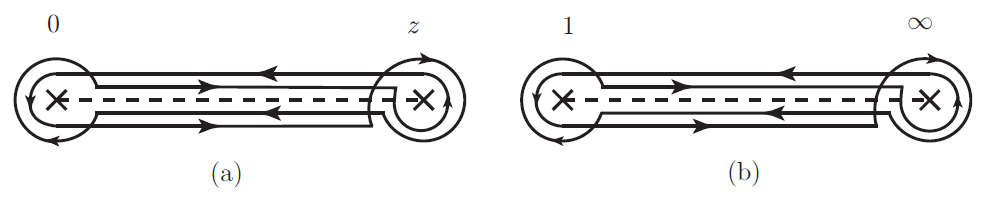
\includegraphics[width=0.6\linewidth]{fig/5.4.png}
	\caption{Pochhammer积分路径,(a)$S_a$,(b)$S_b$。}
\end{figure}

除了带些相位因子, $S_a$ 上的$ I_{S}(z) $就是$ [0,z] $上的积分, $S_b $上的就是 $[1,\infty)$ 上的积分:
\begin{align} &I_{S_{a}}(z)=\left(1-e^{2 \pi i a}\right)\left(1-e^{2 \pi i c}\right) I_{1}(z)\\ &I_{S_{b}}(z)= (1-e^{-2 \pi i(a+b+c)} )\left(1-e^{2 \pi i b}\right) I_{2}(z) \end{align}
其中
\begin{align} I_{1}(z) &=\int_{0}^{z} d v v^{a}(1-v)^{b}(z-v)^{c} \\ &=z^{1+a+b+c} \frac{\Gamma(a+1) \Gamma(c+1)}{\Gamma(a+c+2)} F(-b, a+1, a+c+2 ; z) \\ I_{2}(z) &=\int_{1}^{\infty} d v v^{a}(v-1)^{b}(v-z)^{c} \\ &=\frac{\Gamma(-a-b-c-1) \Gamma(b+1)}{\Gamma(-a-c)} F(-c,-a-b-c-1,-a-c ; z) \end{align}
都可写成超几何级数。借助超几何级数间的关系
\begin{equation}
	F(\alpha, \beta, \gamma ; z)=(1-z)^{\gamma-\alpha-\beta} F(\gamma-\alpha, \gamma-\beta, \gamma ; z) 
\end{equation}
可以看到,在 (5.44) 中取
\begin{equation}
	\alpha_{1}=2\left(\alpha_{0}-\beta_{n_{1}, m_{1}}\right), \quad \alpha_{2}=2\left(\alpha_{0}-\bar{\beta}_{n_{4}, m_{4}}\right), \quad \alpha_{3}=2\left(\alpha_{0}-\beta_{n_{3}, m_{3}}\right)
\end{equation}
得到的就是从$ \phi_{(1,2)} $零模条件推出的微分方程的解。

极小模型的自由场表示是相当有用的工具,可用来研究Virasoro代数的表示,例如构造零模向量,证明Kac的行列式猜想\footnote{M. Kato and S. Matsuda, Adv. Stud. Pure Math. 16 (1988) 205.}\footnote{A. Tsuchiya and Y. Kanie, Publ. RIMS 22 (1986) 259.}\footnote{G. Felder, Nucl. Phys. B 317 (1989) 215 [Erratum-ibid. B 324 (1989) 548].}。本书略过了这些主题,因为例如\footnote{山田泰彦,『共形場理論入門』,培風館, 2006.}\footnote{白石潤一,『量子可積分系入門』,SGC ライブラリ-28,サイエンス社,2003.}\footnote{鈴木淳史,『現代物理数学への招待—ランダムウォークからひろがる多彩な物理と数理』,SGC ライブラリ-47,サイエンス社,2006.}中已经解释得很详细了。

\chapter{环面上的极小模型}
我们先前考虑的共形场论都在复平面上。共形场论也可以定义在一般的二维曲面(Riemann面)上。本章讨论环面上极小模型的配分函数,及其模不变性。

\section{圆柱上的CFT}
\begin{figure}[h]
	\centering
	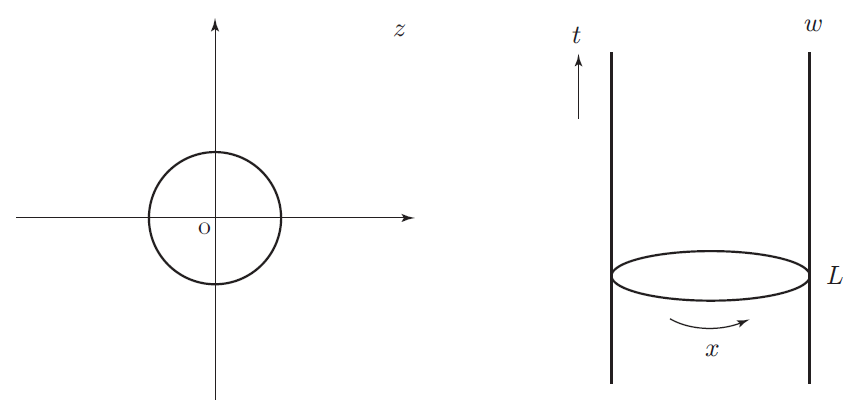
\includegraphics[width=0.6\linewidth]{fig/6.1.png}
	\caption{复平面和圆柱:$z$平面上以原点为圆心的圆,映到$w$平面上固定时刻。}
\end{figure}

考虑周长为 $L $的圆柱上的CFT。时间坐标记作$ t$ ,周向坐标记作 $x$ ,令场 $\phi(t, x) $满足周期性边界条件 $\phi(t, x+L)=\phi(t, x)$ 。坐标$ (t,x)$ 的取值范围是$ -\infty<t<\infty $,$ 0 \leq x \leq L$ 。在有关径向量子化那节(3.3节)解释过,圆柱可通过共形变换映到复平面,如图6.1。复平面上 $z$ 到圆柱上$ w $的共形变换是
\begin{equation}
	w=t+i x=\frac{L}{2 \pi} \log z
\end{equation} 
借助有限共形变换下的变换方程 (3.52) ,可以计算圆柱上CFT中的能动张量 $T_{\mathrm{cyl}}(w)$ 。由
$$
\frac{d w}{d z}=\frac{L}{2 \pi z}, \quad \frac{d^{2} w}{d z^{2}}=\frac{-L}{2 \pi z^{2}}, \quad \frac{d^{3} w}{d z^{3}}=\frac{2 L}{2 \pi z^{3}},
$$
可以得到共形变换 $w=w(z)$ 的Schwarz导数是
$$
S(w, z)=\frac{2-\frac{3}{2}}{z^{2}}=\frac{1}{2 z^{2}}
$$
因此, $z$ 平面上的能动张量$ T(z) $变换为
\begin{equation}
	T_{\text {cyl }}(w)=\left(\frac{2 \pi}{L}\right)^{2}\left(z^{2} T(z)-\frac{c}{24}\right)
\end{equation} 
$c$ 是CFT的中心荷。类似地可得到\footnote{本章考虑$c=\bar{c}$的CFT。如果要求配分函数具有6.3节将讨论的模不变性,可得到$c-\bar{c}$必定是24的整数倍。}
\begin{equation}
	\bar{T}_{\mathrm{cyl}}(\bar{w})=\left(\frac{2 \pi}{L}\right)^{2}\left(\bar{z}^{2} \bar{T}(\bar{z})-\frac{c}{24}\right) 
\end{equation}

圆柱上的Hamiltonian算符$ H $,是时间 $t$ 方向上的演化算符,也是Hamiltonian密度$ T_{t t}(t, x)=T_{\mathrm{cyl}}(w)+\bar{T}_{\mathrm{cyl}}(\bar{w})$ 的空间积分
\begin{equation}
	H=\frac{1}{2 \pi} \int_{0}^{L} T_{t t}(t, x) d x 
\end{equation}
与此类似,圆柱上的动量算符$ P $,是空间 $x$ 方向上的平移算符,也是动量密度 $T_{t x}(t,x)=i\left(T_{\mathrm{cyl}}(w)-\bar{T}_{\mathrm{cyl}}(\bar{w})\right)$ 的空间积分
\begin{equation}
	P=\frac{1}{2 \pi} \int_{0}^{L} \frac{1}{i} T_{t x}(t, x) d x 
\end{equation}
将$ T(z), \bar{T}(\bar{z}) $的模式展开 (3.56) 代入 (6.2),(6.3) ,得到
\begin{align} &T_{\mathrm{cyl}}(w)=\left(\frac{2 \pi}{L}\right)^{2}\left(\sum_{n=-\infty}^{\infty} L_{n} e^{-\frac{2 \pi n}{L}(t+i x)}-\frac{c}{24}\right) \\ &\bar{T}_{\mathrm{cyl}}(\bar{w})=\left(\frac{2 \pi}{L}\right)^{2}\left(\sum_{n=-\infty}^{\infty} \bar{L}_{n} e^{-\frac{2 \pi n}{L}(t-i x)}-\frac{c}{24}\right) \end{align}
作空间积分的话,将只剩下零模$ L_{0}, \bar{L}_{0}$ ,得到Hamiltonian和动量算符是
\begin{align} &H=\frac{2 \pi}{L}\left(L_{0}+\bar{L}_{0}\right)-\frac{\pi c}{6 L}\\ &P=\frac{2 \pi}{L}\left(L_{0}-\bar{L}_{0}\right) \end{align}
共形权为 $(h, \bar{h}) $的初级场$ \phi(z, \bar{z}) $的最高权态 $|h, \bar{h}\rangle $是$ H,P$的本征态,本征值是
\begin{equation}
H=\frac{2 \pi}{L}(h+\bar{h})-\frac{\pi c}{6 L}, \quad P=\frac{2 \pi}{L}(h-\bar{h})
\end{equation} 
$x_{\phi}=h+\bar{h}$ 称为 $\phi $的\textbf{共形维数}, $s=h-\bar{h} $称为 $\phi$ 的\textbf{自旋}。

\section{环面上的CFT}
\subsection{配分函数}
考虑周长 $L $,高 $M$ 的圆柱。在空间和时间方向都要求场 $\phi(t,x)$ 满足周期性边界条件: $\phi(t, x+L)=\phi(t, x)$ , $\phi(t+M, x)=\phi(t, x) $。这个CFT的配分函数是
\begin{equation}
\begin{aligned} Z(L, M) &=\operatorname{Tr} \exp (-M H) \\ &=\operatorname{Tr} \exp \left\{-\frac{2 \pi M}{L}\left(L_{0}+\bar{L}_{0}-\frac{c}{12}\right)\right\} 	
\end{aligned}
\end{equation}
这里的迹是在所考虑CFT的Hilbert空间中取的。

\begin{figure}[h]
	\centering
	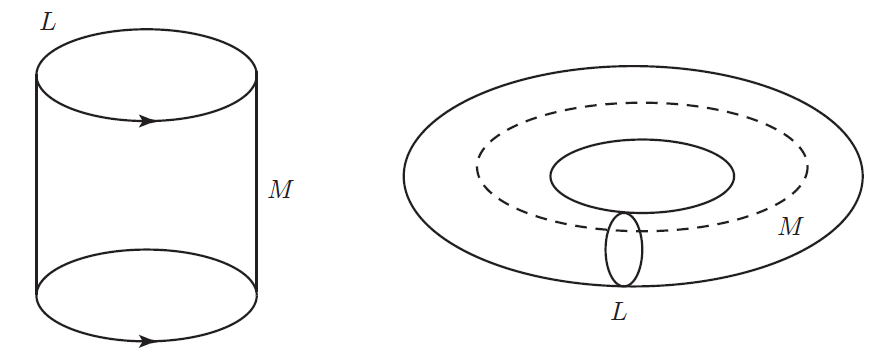
\includegraphics[width=0.6\linewidth]{fig/6.2.png}
	\caption{圆柱和环面:圆柱的上下两端粘起来得到环面。}
\end{figure}

定义CFT的二维曲面是个环面,通过将圆柱的上下两端粘起来得到,如图6.2。环面也可通过取长为 $L,M $的矩形,将左右两端和上下两端粘起来得到,如图6.3。

\begin{figure}[h]
	\centering
	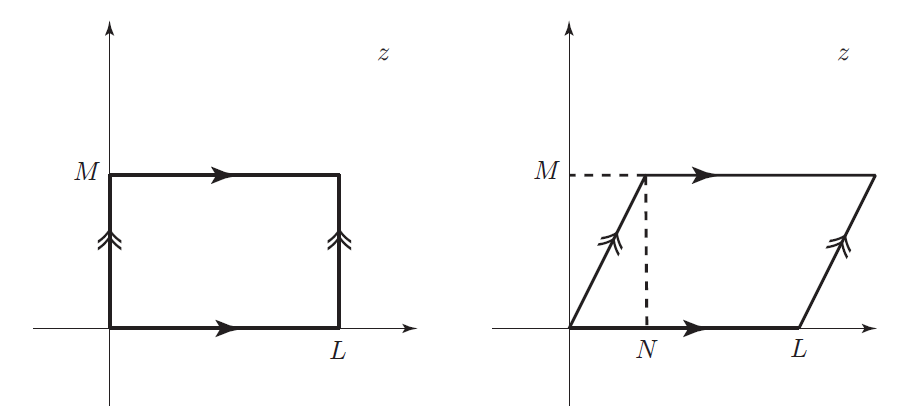
\includegraphics[width=0.6\linewidth]{fig/6.3.png}
	\caption{复平面上的矩形或平行四边形,对边粘起来得到环面。}
\end{figure}

粘起上下两端时,可先令上端转过弧长 $N$ 。这样就在配分函数的迹中,插入了 $x $方向上的平移算符 $\exp (i N P)$ :
\begin{equation}
	\begin{aligned} Z\left(\omega_{1}, \omega_{2}\right) &=\operatorname{Tr} \exp (-M H+i N P) \\ &=\operatorname{Tr} \exp \left\{-\frac{2 \pi M}{L}\left(L_{0}+\bar{L}_{0}-\frac{c}{12}\right)+2 \pi i \frac{N}{L}\left(L_{0}-\bar{L}_{0}\right)\right\} \end{aligned}
\end{equation}
$\omega_{1}=L $,$ \omega_{2}=N+i M$ 是在复平面上表示环面时,描述几何(两顶点的位置)的参数,称为周期。环面可通过将复 z 平面上满足 $z_{1}-z_{2}=n \omega_{1}+m \omega_{2} $( $n,m $是整数)的两点 $z_1,z_2 $视作等价得到。

配分函数可写成
\begin{equation}
	Z(\tau, \bar{\tau})=\operatorname{Tr} q^{L_{0}-\frac{c}{24}} \bar{q}^{\bar{L}_{0}-\frac{c}{24}}
\end{equation} 
其中
\begin{equation}
	q=\exp (2 \pi i \tau), \quad \bar{q}=\exp (-2 \pi i \bar{\tau}), \quad \tau=\frac{\omega_{2}}{\omega_{1}} 
\end{equation}
配分函数依赖于几何参数 $\omega_1,\omega_2 $之比。换句话说,它不依赖于环面的尺寸。复参数$ \tau $称为环面的模参数。

CFT的Hilbert空间可分解成Virasoro代数最高权为 $(h, \bar{h}) $的不可约表示 $V_{h} \otimes \bar{V}_{\bar{h}} $之和。Hilbert空间分解中 $V_{h} \otimes \bar{V}_{\bar{h}}$ 出现的次数记作$ N_{h, \bar{h}} $,那么配分函数可写成
\begin{equation}
	Z(\tau, \bar{\tau})=\sum_{h, \bar{h}} N_{h, \bar{h}} \chi_{(c, h)}(q) \chi_{(c, \bar{h})}(\bar{q})
\end{equation} 
其中
\begin{equation}
	\chi_{(c, h)}(q)=\operatorname{Tr}_{V_{h}} q^{L_{0}-\frac{c}{24}} 
\end{equation}
的迹是在Virasoro代数的不可约表示 $V_h $中取的,称为$ V_h$ 的\textbf{特征标}。类似地,$ \bar{V}_{\bar{h}} $的特征标是
\begin{equation}
	\chi_{(c, \bar{h})}(\bar{q})=\operatorname{Tr}_{\bar{V}_{\bar{h}}} \bar{q}^{\bar{L}_{0}-\frac{c}{24}} 
\end{equation}

\subsection{Virasoro代数的特征标}

Virasoro代数最高权为$ h $的表示 $V_h $中的态由 $L_0 $的本征值标记。级为 $N$ 的态张成的 $V_h$ 的子空间记作 $V_{h, N} $,是 $L_0 $的本征值为 $h+N$ 的本征空间。因为级为 $N$ 的线性独立态的数目等于$ V_{h, N} $的维数 $\operatorname{dim} V_{h, N} $,特征标是
\begin{equation}
	\chi_{(c, h)}(q)=q^{-\frac{c}{24}} \sum_{N=0}^{\infty} \operatorname{dim} V_{h, N} q^{h+N} 
\end{equation}
如果$ V_h$ 不含零模态,也就是说,如果最高权态$ |h\rangle$ 和它的次级态张成的Verma模$ V_h$ 是Virasoro代数的不可约表示,那么级为$ N $的态的数目 $\operatorname{dim} V_{h, N} $,就等于 $N$ 的拆分数 $p(N)$ ,因此特征标是
\begin{equation}
	\chi_{(c, h)}(q)=q^{-\frac{c}{24}} \sum_{N=0}^{\infty} p(N) q^{h+N}=\frac{q^{h-\frac{c}{24}}}{P(q)}
\end{equation} 
其中,$ P(q)=\prod_{n=1}^{\infty}\left(1-q^{n}\right)$ 由 (5.94) 定义。

如果 $V_h$ 含一个级为$ L $的零模态 $|h+L\rangle $,$ V_h $中定义等价关系 $|h+L\rangle=0 $得到的空间 $[h]=V_{h} / V_{h+L}$ 是不可约表示。这时,Verma模 $V_h $的特征标$ \operatorname{Tr}_{V_{h}} q^{L_{0}-\frac{c}{24}}$ ,减去零模态张成的子空间 $V_{h+L} $的特征标$ \operatorname{Tr}_{V_{h+L}} q^{L_{0}-\frac{c}{24}} $,才是不可约表示的特征标
\begin{equation}
\begin{aligned} \chi_{(c, h)}(q) &=q^{-\frac{c}{24}} \sum_{N=0}^{\infty}\left(\operatorname{dim} V_{h, N} q^{h+N}-\operatorname{dim} V_{h+L, N} q^{h+L+N}\right) \\ &=\frac{q^{h-\frac{c}{24}}\left(1-q^{L}\right)}{P(q)} \end{aligned}
\end{equation}

\subsection{极小模型的特征标}

考虑中心荷为$ c=1- 6(p-q)^{2}/(p q) $( $p,q $是互素正整数, $p>q$ )的极小模型的特征标\footnote{不要混淆这里的$q$和模参数$\tau$的函数$q=\exp (2\pi i \tau)$。}\footnote{A. Rocha-Caridi, “Vacuum Vector Representations of the Virasoro Algebra”, in Vertex Operators in Mathematics and Physics, MSRI Publications No.3, Springer, 1984.}。共形权为 $h_{n,m}= [(n p-m q)^{2}-(p-q)^{2}]/(4 p q) $的初级场$ \phi_{(n, m)} $( $0<n<q $,$ 0<m<p$ )对应的最高权表示记作$ \left[h_{n, m}\right] $。5.4节解释过,其中有级为 $nm $的零模态 $\left|h_{q-n, p+m}\right\rangle$和级为 $(q-n)(p-m) $的零模态$ \left|h_{2 q-n, m}\right\rangle $。但[由 (5.29) ]可以发现,Verma模$ V_{h_{q-n, p+m}}$ 和$ V_{h_{2 q-n, m}} $含共同的零模态$ \left|h_{2 q+n, m}\right\rangle $和 $\left|h_{3 q-n, p-m}\right\rangle $,那么从这些态生成的Verma模$ V_{h_{2 q+n, m}} \oplus V_{h_{3 q-n, p-m}} $就有两份。这种零模态无穷嵌套的结构如图6.4。

\begin{figure}[h]
	\centering
	\begin{tikzcd}[column sep=tiny]
		& {h_{n,m}} \arrow[ld] \arrow[rd] &                                           \\
		{h_{2q-n,m}} \arrow[rrd] \arrow[d]  &                                 & {h_{q+n,p-m}} \arrow[lld] \arrow[d]       \\
		{h_{3q-n,p-m}}                      &                                 & {h_{2q+n,m}}                              \\
		\vdots                              &                                 & \vdots                                    \\
		{h_{2qk-n,m}} \arrow[d] \arrow[rrd] &                                 & {h_{(2k-1)q+n,p-m}} \arrow[d] \arrow[lld] \\
		{h_{(2k+1)q-n,p-m}}                 &                                 & {h_{2kq+n,m}}                             \\
		\vdots                              &                                 & \vdots                                   
	\end{tikzcd}
	\caption{最高权表示$[h_{n,m}]$中零模态无穷嵌套的结构。}
\end{figure}

根据这样的结构,最高权表示$ \left[h_{n, m}\right] $的特征标是
\begin{equation}
	\begin{aligned} \chi_{\left(c, h_{n, m}\right)}(\tau)=& \frac{q^{-\frac{c}{24}}}{P(q)}\left\{q^{h_{n, m}}-\sum_{k=1}^{\infty}\left(q^{h_{2 k q-n, m}}+q^{h_{(2 k-1) q+n, p-m}}\right)\right.\\&\left.+\sum_{k=1}^{\infty}\left(q^{h_{(2 k+1) q-n, p-m}}+q^{h_{2 k q+n, m}}\right)\right\} \end{aligned}
\end{equation}
可借助$ h_{n, m}=h_{q-n, p-m}$ 改写成
\begin{equation}
	\begin{aligned} \chi_{\left(c, h_{n, m}\right)}(\tau)=& \frac{q^{-\frac{c}{24}}}{P(q)}\left\{\sum_{k=-\infty}^{\infty}\left(q^{h_{2 k q+n, m}}-q^{h_{2 k q-n, m}}\right)\right\} \\ =&\frac{q^{-\frac{c}{24}}}{P(q)}\left\{\sum_{k=-\infty}^{\infty} \left(q^{\left[(2 k p q+m q-n p)^{2}-(p-q)^{2}\right] /(4 p q)}-q^{\left[(2 k p q+m q+n p)^{2}-(p-q)^{2}\right] /(4 p q)}\right)\right\} \end{aligned}
\end{equation} 

现在来看一些具体的例子。 $(p,q)=(3,2) $时, $c=0 $, $h_{1,1}=0 $的最高权表示只含$ |0\rangle $,因此 $\chi_{\left(c=0, h_{1,1}=0\right)}(q)=1 $。另一方面,代入 (6.22) 给出
\begin{equation}
	\chi_{(0,0)}(q)=\frac{1}{P(q)} \sum_{k=-\infty}^{\infty}(-1)^{k} q^{\frac{3 k^{2}+k}{2}} 
\end{equation}
由此推出
\begin{equation}
	\prod_{n=1}^{\infty}\left(1-q^{n}\right)=\sum_{k=-\infty}^{\infty}(-1)^{k} q^{\frac{3 k^{2}+k}{2}} 
\end{equation}
这可通过在下子节将介绍的Jacobi三重积公式
\begin{equation}
	\prod_{n=1}^{\infty}\left(1-q^{2 n}\right)\left(1-y^{-1} q^{2 n-1}\right)\left(1-y q^{2 n-1}\right)=\sum_{k=-\infty}^{\infty}(-1)^{k} y^{k} q^{k^{2}}
\end{equation} 
中令 $q \rightarrow q^{\frac{3}{2}} $,$ y \rightarrow q^{\frac{1}{2}}$ 得到。

对Ising模型, $(p, q)=(4,3)$ ,有共形权为 $h_{1,1}=0 $,$ h_{1,2}=1/16$ ,$ h_{1,3}=1/2 $的初级场,相应的最高权表示特征标是
\begin{align} &\chi_{\left(\frac{1}{2}, 0\right)}(q)=\frac{q^{-\frac{1}{48}}}{P(q)} \sum_{k=-\infty}^{\infty}\left(q^{\frac{\left[(24 k+1)^{2}-1\right]}{48}}-q^{\frac{\left[(24 k+7)^{2}-1\right]}{48}}\right) \\ &\chi_{\left(\frac{1}{2}, \frac{1}{2}\right)}(q)=\frac{q^{-\frac{1}{48}}}{P(q)} \sum_{k=-\infty}^{\infty}\left(q^{\frac{\left[(24 k+5)^{2}-1\right]}{48}}-q^{\frac{\left[(24 k+11)^{2}-1\right]}{48}}\right) \\ &\chi_{\left(\frac{1}{2}, \frac{1}{16}\right)}(q)=\frac{q^{-\frac{1}{48}}}{P(q)} \sum_{k=-\infty}^{\infty}\left(q^{\frac{\left[(24 k-2)^{2}-1\right]}{48}}-q^{\frac{\left[(24 k+10)^{2}-1\right]}{48}}\right) \end{align}
令 $r=4k $,$ s=4k+1 $, (6.26) 可改写成
\begin{equation}
	\chi_{\left(\frac{1}{2}, 0\right)}(q)=\frac{q^{-\frac{1}{48}}}{P(q)}\left( \sum_{r\equiv 0\ (\text{mod}\ 4)\in \mathbb{Z}} q^{\frac{3 r^{2}+r}{4}}-\sum_{s\equiv 1\ (\text{mod}\ 4)\in \mathbb{Z}} \quad q^{\frac{3 s^{2}+s}{4}}\right)
\end{equation} 
类似地有
\begin{align} &\chi_{\left(\frac{1}{2}, \frac{1}{2}\right)}(q)=\frac{q^{-\frac{1}{48}}}{P(q)}\left( \sum_{r\equiv 1\ (\text{mod}\ 4)\in \mathbb{Z}} q^{\frac{3 r^{2}-r}{4}}-\sum_{s\equiv 2\ (\text{mod}\ 4)\in \mathbb{Z}}q^{\frac{3s^2-s}{4}}\right)\\ &\chi_{\left(\frac{1}{2}, \frac{1}{16}\right)}(q)=\frac{q^{-\frac{1}{48}}}{P(q)} \sum_{k=-\infty}^{\infty}(-1)^{k} q^{3 k^{2}+k} \end{align}
在 (6.24) 中令 $4q\to q^2$ ,可得到
\begin{equation}
	\sum_{k=-\infty}^{\infty}(-1)^{k} q^{3 k^{2}+k}=\prod_{n=1}^{\infty}\left(1-q^{2 n}\right)=P(q) \prod_{n=1}^{\infty}\left(1+q^{n}\right) 
\end{equation}
于是 (6.31) 可写成无穷乘积。至于另两个特征标,考虑线性组合 $\chi_{\left(\frac{1}{2}, 0\right)}(q) \pm \chi_{\left(\frac{1}{2}, \frac{1}{2}\right)}(q)$ ,我们有
\begin{align} &\chi_{\left(\frac{1}{2}, 0\right)}(q)-\chi_{\left(\frac{1}{2}, \frac{1}{2}\right)}(q)=\frac{q^{-\frac{1}{48}}}{P(q)} \sum_{k=-\infty}^{\infty}(-1)^{k} q^{\frac{3 k^{2}+k}{4}} \\ &\chi_{\left(\frac{1}{2}, 0\right)}(q)+\chi_{\left(\frac{1}{2}, \frac{1}{2}\right)}(q)=\frac{q^{-\frac{1}{48}}}{P(q)} \sum_{k=-\infty}^{\infty}(-1)^{\frac{3 k(k+1)}{2}} q^{\frac{3 k^{2}+k}{4}}\end{align}
在Jacobi三重积公式 (6.25) 中令$q \rightarrow q^{\frac{3}{4}} $,$ y \rightarrow q^{\frac{1}{4}} $,可得到
\begin{align} &\sum_{k=-\infty}^{\infty}(-1)^{k} q^{\frac{3 k^{2}+k}{4}}=P(q) \prod_{n=0}^{\infty} (1-q^{n+\frac{1}{2}} ) \\& \sum_{k=-\infty}^{\infty}(-1)^{\frac{3 k(k+1)}{2}} q^{\frac{3 k^{2}+k}{4}}=P(q) \prod_{n=0}^{\infty} (1+q^{n+\frac{1}{2}} ) \end{align}
第二条式子是在第一条式子中令$ q \rightarrow e^{2 \pi i} q $得到的。最终,我们得到了Ising模型特征标的无穷乘积表示:
\begin{align} &\chi_{\left(\frac{1}{2}, 0\right)}(q)=\frac{q^{-\frac{1}{48}}}{2}\left\{\prod_{n=0}^{\infty} (1+q^{n+\frac{1}{2}} )+\prod_{n=0}^{\infty} (1-q^{n+\frac{1}{2}} )\right\} \\ &\chi_{\left(\frac{1}{2}, \frac{1}{2}\right)}(q)=\frac{q^{-\frac{1}{48}}}{2}\left\{\prod_{n=0}^{\infty} (1+q^{n+\frac{1}{2}} )-\prod_{n=0}^{\infty} (1-q^{n+\frac{1}{2}} )\right\} \\ &\chi_{\left(\frac{1}{2}, \frac{1}{16}\right)}(q)=q^{-\frac{1}{48}} \prod_{n=1}^{\infty}\left(1+q^{n}\right) \end{align}
这种无穷乘积表示,对应用自由费米子写的Ising模型CFT。

\subsection{theta函数}

Virasoro代数的特征标可写成模参数 $\tau $的函数$ q=\exp (2 \pi i \tau) $的无穷级数,但其中最基本的结构是Jacobi theta函数$ \vartheta_{a}(z, \tau) $( $a=1,2,3,4 $)。$ z$是复数,$ \tau$ 是满足$ \operatorname{Im} \tau>0 $的复数。本子节用于总结theta函数的基本性质,更详细的讲解见例如\footnote{A. フルヴィッツ,R. クーラント,『楕円関数論』,足立恒雄,小松啓一訳,シュプリンガー・フェ アラーク東京,1991.}\footnote{D. Mumford, Tata Lectures on Theta I, Birkhäuser, 2006.}。
它们的定义是
\begin{align} &\vartheta_{1}(z, \tau)=i \sum_{n=-\infty}^{\infty}(-1)^{n} q^{\frac{1}{2}\left(n-\frac{1}{2}\right)^{2}} e^{i \pi(2 n-1) z} \\ &\vartheta_{2}(z, \tau)=\sum_{n=-\infty}^{\infty} q^{\frac{1}{2}\left(n-\frac{1}{2}\right)^{2}} e^{i \pi(2 n-1) z} \\ &\vartheta_{3}(z, \tau)=\sum_{n=-\infty}^{\infty} q^{\frac{n^{2}}{2}} e^{2 i \pi n z} \\ &\vartheta_{4}(z, \tau)=\sum_{n=-\infty}^{\infty}(-1)^{n} q^{\frac{n^{2}}{2}} e^{2 i \pi n z} \end{align}
只有 $\vartheta_{1}(z, \tau) $是奇函数:
\begin{align} &\vartheta_{1}(-z, \tau)=-\vartheta_{1}(z, \tau) \\ &\vartheta_{a}(-z, \tau)=\vartheta_{a}(z, \tau) \quad(a=2,3,4) \end{align}
特别地,可以看到 $z=0$ 是 $\vartheta_{1}(z, \tau) $的零点。此外,在平移变换 $z \rightarrow z+1/2$ 和 $z \rightarrow z+ \tau/2 $下我们有
\begin{align} &\vartheta_{1}\left(z+\frac{1}{2}, \tau\right)=\vartheta_{2}(z, \tau)\\ &\vartheta_{2}\left(z+\frac{1}{2}, \tau\right)=-\vartheta_{1}(z, \tau)\\ &\vartheta_{3}\left(z+\frac{1}{2}, \tau\right)=\vartheta_{4}(z, \tau)\\ &\vartheta_{4}\left(z+\frac{1}{2}, \tau\right)=\vartheta_{3}(z, \tau) \\ &\vartheta_{1}\left(z+\frac{\tau}{2}, \tau\right)=i q^{\frac{1}{8}} e^{-\pi i z} \vartheta_{4}(z, \tau)\\ &\vartheta_{2}\left(z+\frac{\tau}{2}, \tau\right)=q^{\frac{1}{8}} e^{-\pi i z} \vartheta_{3}(z, \tau)\\ &\vartheta_{3}\left(z+\frac{\tau}{2}, \tau\right)=q^{-\frac{1}{8}} e^{-\pi i z} \vartheta_{2}(z, \tau)\\ &\vartheta_{4}\left(z+\frac{\tau}{2}, \tau\right)=i q^{-\frac{1}{8}} e^{-\pi i z} \vartheta_{1}(z, \tau)  \end{align}
将它们复合起来,得到
\begin{align} &\vartheta_{1}\left(z+\frac{1}{2}+\frac{\tau}{2}, \tau\right)=q^{\frac{1}{8}} e^{-\pi i z} \vartheta_{3}(z, \tau) \\ &\vartheta_{2}\left(z+\frac{1}{2}+\frac{\tau}{2}, \tau\right)=-i q^{\frac{1}{8}} e^{-\pi i z} \vartheta_{4}(z, \tau) \\ &\vartheta_{3}\left(z+\frac{1}{2}+\frac{\tau}{2}, \tau\right)=i q^{-\frac{1}{8}} e^{-\pi i z} \vartheta_{1}(z, \tau) \\ &\vartheta_{4}\left(z+\frac{1}{2}+\frac{\tau}{2}, \tau\right)=q^{-\frac{1}{8}} e^{-\pi i z} \vartheta_{2}(z, \tau) \end{align}
在平移变换$ z \rightarrow z+n+m \tau $下, $\vartheta_{a}(z, \tau) $的值和原来只相差一个数值因子。从 $\vartheta_{a}(z, \tau) $的这一准周期性,可以推出 $\vartheta_{1}(z, \tau)$ 的零点是
$$
z=n+m \tau, \quad n, m \in \mathbb{Z}
$$
$\vartheta_{2}(z, \tau) $, $\vartheta_{3}(z, \tau) $和 $\vartheta_{4}(z, \tau) $的零点,则是 $\vartheta_{1}(z, \tau)$ 的零点分别平移 $1/2$ , $(1+\tau)/2$ 和 $\tau/2 $。引入变量 $y=e^{2 \pi i z} $,那么 $\vartheta_{1}(z, \tau)$ 的零点是 $y=q^{m} $( $m\in \mathbb{Z} $),它有无穷乘积形式
$$
\vartheta_{1}(z, \tau)=2 i C q^{\frac{1}{8}} \sin \pi z \prod_{m=1}^\infty\left(1-y q^{m}\right)\left(1-y^{-1} q^{m}\right)
$$
$C$ 是不依赖于$ z $的数,我们不讨论如何确定 $C$ ,可见\footnote{A. フルヴィッツ,R. クーラント,『楕円関数論』,足立恒雄,小松啓一訳,シュプリンガー・フェ アラーク東京,1991.}。最终的结果是
\begin{align} &\vartheta_{1}(z, \tau)=i 2 e^{\frac{\pi i \tau}{4}} \sin \pi z \prod_{m=1}^{\infty}\left(1-q^{m}\right)\left(1-y q^{m}\right)\left(1-y^{-1} q^{m}\right) \\ &\vartheta_{2}(z, \tau)=2 e^{\frac{\pi i \tau}{4}} \cos \pi z \prod_{m=1}^{\infty}\left(1-q^{m}\right)\left(1+y q^{m}\right)\left(1+y^{-1} q^{m}\right) \\ &\vartheta_{3}(z, \tau)=\prod_{m=1}^{\infty}\left(1-q^{m}\right) (1+y q^{m-\frac{1}{2}} ) (1+y^{-1} q^{m-\frac{1}{2}} ) \\ &\vartheta_{4}(z, \tau)=\prod_{m=1}^{\infty}\left(1-q^{m}\right) (1-y q^{m-\frac{1}{2}}) (1-y^{-1} q^{m-\frac{1}{2}} ) \end{align}
这里, $\vartheta_{4}(z, \tau) $的无穷乘积表示,正是Jacobi三重积公式 (6.25) 中令 $q \rightarrow q^{\frac{1}{2}} $。

接着引入Dedekind eta函数
\begin{equation}
	\eta(\tau)=q^{\frac{1}{24}} P(q)=q^{\frac{1}{24}} \prod_{n=1}^{\infty}\left(1-q^{n}\right), \quad q=e^{2 \pi i \tau}
\end{equation} 
代入 (6.24) 可得到
\begin{equation}
	\eta(\tau)=\sum_{k=-\infty}^{\infty}(-1)^{k} q^{\frac{3}{2}\left(k+\frac{1}{6}\right)^{2}}
\end{equation} 

Ising模型的特征标可用theta和eta函数表示。借助无穷乘积表示
\begin{equation}
	\begin{aligned} \frac{\vartheta_{3}(0, \tau)}{\eta(\tau)} &=\frac{\prod_{m=1}^{\infty}\left(1-q^{m}\right) (1+q^{m-\frac{1}{2}} ) (1+q^{m-\frac{1}{2}} )}{q^{\frac{1}{24}} \prod_{m=1}^{\infty}\left(1-q^{m}\right)} \\ &=q^{-\frac{1}{24}} \prod_{m=1}^{\infty} (1+q^{m-\frac{1}{2}} )^{2} \end{aligned} 
\end{equation}
类似地有
\begin{align} &\frac{\vartheta_{4}(0, \tau)}{\eta(\tau)}=q^{-\frac{1}{24}} \prod_{m=1}^{\infty} (1-q^{m-\frac{1}{2}} )^{2}\\ &\frac{\vartheta_{2}(0, \tau)}{\eta(\tau)}=2 q^{\frac{1}{12}} \prod_{m=0}^{\infty}\left(1+q^{m}\right)^{2}\end{align}
与 (6.37),(6.38),(6.39) 比对可知,
\begin{align} & \chi_{\left(\frac{1}{2}, 0\right)}(q)=\frac{1}{2}\left(\sqrt{\frac{\vartheta_{3}(0, \tau)}{\eta(\tau)}}+\sqrt{\frac{\vartheta_{4}(0, \tau)}{\eta(\tau)}}\right) \\ &\chi_{\left(\frac{1}{2}, \frac{1}{2}\right)}(q)=\frac{1}{2}\left(\sqrt{\frac{\vartheta_{3}(0, \tau)}{\eta(\tau)}}-\sqrt{\frac{\vartheta_{4}(0, \tau)}{\eta(\tau)}}\right) \\ &\chi_{\left(\frac{1}{2}, \frac{1}{16}\right)}(q)=\frac{1}{\sqrt{2}} \sqrt{\frac{\vartheta_{2}(0, \tau)}{\eta(\tau)}} \end{align}
再引入theta函数($ A_1^{(1)} $经典theta函数\footnote{V. G. Kac, Infinite-Dimensional Lie Algebra, 3rd ed., Cambridge Univ. Press, 1990.}\footnote{脇本実,『無限次元リー環』,岩波書店,2008.})
\begin{equation}
	\begin{aligned} &\Theta_{n, m}(z, \tau, u)=e^{2 \pi i m u} \sum_{k=-\infty}^{\infty} e^{2 \pi i m\left(\left(k+\frac{n}{2 m}\right)^{2} \tau+\left(k+\frac{n}{2 m}\right) z\right)}, \\ &n \equiv 0, \cdots, 2 m-1 \quad(\text{mod}\ 2 m) \end{aligned} 
\end{equation}
特别地,为讨论 $(p,q) $极小模型的特征标,我们需要$ u=0$ 情形,因此定义
\begin{equation}
	\begin{aligned} &\Theta_{n, m}(z, \tau)=\sum_{k=-\infty}^{\infty} q^{m\left(k+\frac{n}{2 m}\right)^{2}} e^{2 \pi i m\left(k+\frac{n}{2 m}\right) z} ,\\ &n \equiv 0, \cdots, 2 m-1 \quad(\text{mod}\ 2 m) \end{aligned}
\end{equation}
在 $(p,q) $极小模型的特征标 (6.22) 中代入中心荷$ c=1- 6(p-q)^{2}/(p q)$ ,可得到
\begin{equation}
	\chi_{\left(c, h_{n, m}\right)}(\tau)=K_{\lambda_{n, m}}(\tau)-K_{\lambda_{n,-m}}(\tau) 
\end{equation}
其中
\begin{align} &K_{\lambda}(\tau)=\frac{1}{\eta(\tau)} \Theta_{\lambda, \frac{N}{2}}(0, \tau)\\ & N=2 p q \\ & \lambda_{n, m}=n p-m q  \end{align}

\section{配分函数的模不变性}
因为$ SL(2,\mathbb{Z}) $模变换不改变环面的形状,环面上的配分函数 $Z(\tau, \bar{\tau}) $是模不变的。这对极小模型的结构和四点函数的单值变换不变性施加了很强的限制。为讨论特征标在模变换下的行为,需要进一步的数学基础,我们现在就来解释。

\subsection{ 环面的模变换}

环面可定义为复平面上的二维格。考虑两向量 $\omega_1,\omega_2$ 生成的二维格。假定复数 $\tau=\omega_2/\omega_1 $的虚部为正。$ \tau $称为模参数。环面可通过将复平面上平移 $z \rightarrow z+n \omega_{1}+m \omega_{2}$ ( $n,m$ 是整数)前后的两点视作等价得到。

\begin{figure}[h]
	\centering
	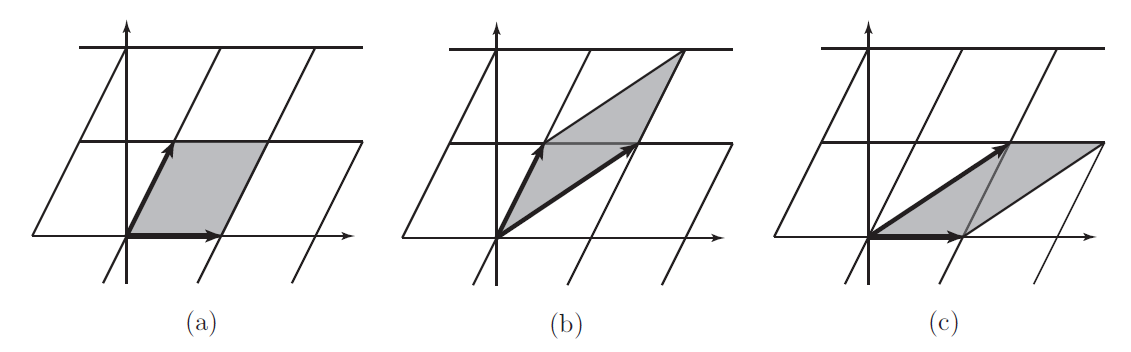
\includegraphics[width=0.6\linewidth]{fig/6.5.png}
	\caption{(a) $(\omega_1,\omega_2)$,(b)$(\omega_1+\omega_2,\omega_2)$,(c) $(\omega_1,\omega_1+\omega_2)$为周期的环面。}
\end{figure}

生成格的基 $(\omega_1,\omega_2) $取法不唯一。例如, $\left(\omega_{1}, \omega_{1}+\omega_{2}\right)$ 和 $\left(\omega_{1}+\omega_{2}, \omega_{2}\right) $也生成同样的格,如图6.5。模参数在这基变换下变为:
\begin{align} &T: \tau \rightarrow \tau+1 \\ &U: \tau \rightarrow \frac{\tau}{\tau+1} \end{align}
定义 $S$ 变换为
\begin{equation}
	S: \tau \rightarrow-\frac{1}{\tau}
\end{equation} 
我们有 $U=T S T $。

考虑一般的基变换
\begin{equation}
	\left(\begin{array}{l} \omega_{2} \\ \omega_{1} \end{array}\right) \rightarrow\left(\begin{array}{l} \omega_{2}^{\prime} \\ \omega_{1}^{\prime} \end{array}\right)=\left(\begin{array}{ll} a & b \\ c & d \end{array}\right)\left(\begin{array}{l} \omega_{2} \\ \omega_{1} \end{array}\right)
\end{equation}
如果前后的两基生成同样的格,那么$ a,b,c,d $要是整数,且 $a d-b c=1 $。换句话说,矩阵
\begin{equation}
	\left(\begin{array}{ll} a & b \\ c & d \end{array}\right) 
\end{equation}
描述的线性变换,要是 $P S L(2, \mathbb{Z})=S L(2, \mathbb{Z}) / \mathbb{Z}_{2} $的元素。模参数在这基变换下变为:
\begin{equation}
	\tau \rightarrow \frac{a \tau+b}{c \tau+d} 
\end{equation}\quad \quad (6.81)
$\mathbb{Z}_2$ 中恒等变换之外的元素,由矩阵
\begin{equation}
	\left(\begin{array}{cc} -1 & 0 \\ 0 & -1 \end{array}\right) 
\end{equation}\quad \quad (6.82)
描述。对模参数来说,它和恒等变换的效果一样。换句话说,矩阵乘上 $-1 $,和原来视作等价。$ P S L(2, \mathbb{Z}) $可由 $T $变换和 $S $变换生成。可以验证矩阵
$$
S=\left(\begin{array}{ll} 0 & -1 \\ 1 & 0 \end{array}\right)
$$
和
$$
T=\left(\begin{array}{ll} 1 & 1 \\ 0 & 1 \end{array}\right)
$$
满足
\begin{equation}
	S^{2}=1, \quad(S T)^{3}=1
\end{equation} \quad \quad (6.83)

\subsection{ Poisson公式}
实数$ x$ 的函数$ f(x)$ 的Fourier变换是
\begin{equation}
	\tilde{f}(y)=\int_{-\infty}^{\infty} e^{-2 \pi i y x} f(x) d x
\end{equation} 
考虑 $f(x) $定义的无穷求和
\begin{equation}
F(x)=\sum_{n=-\infty}^{\infty} f(x+n)	
\end{equation}
$F(x) $具有周期性$ F(x+1)=F(x)$ ,因此可写成Fourier级数
\begin{equation}
	F(x)=\sum_{m=-\infty}^{\infty} F_{m} e^{2 \pi i m x}
\end{equation} 
系数是
\begin{equation}
	F_{m}=\int_{0}^{1} d x e^{-2 \pi i m x} F(x) 
\end{equation}
代入 (6.85) 得到
\begin{equation}
	\begin{aligned} F_{m} &=\sum_{n=-\infty}^{\infty} \int_{0}^{1} e^{-2 \pi i m x} f(x+n) d x \\ &=\sum_{n=-\infty}^{\infty} \int_{n}^{n+1} e^{-2 \pi i m\left(x^{\prime}-n\right)} f\left(x^{\prime}\right) d x^{\prime} \quad\left(令x^{\prime}=x+n \right) \\ &=\int_{-\infty}^{\infty} e^{-2 \pi i m x^{\prime}} f\left(x^{\prime}\right) d x^{\prime} \end{aligned}
\end{equation}
也就是说,Fourier系数$ F_m$ 等于$ f(x) $的Fourier变换 $\tilde{f}(y)$ 在 $y=m $时的值 $\tilde{f}(m)$ 。因此
\begin{equation}
	\sum_{n=-\infty}^{\infty} f(x+n)=\sum_{m=-\infty}^{\infty} \tilde{f}(m) e^{2 \pi i m x}
\end{equation}
令$ x=0 $得到
\begin{equation}
	\sum_{n=-\infty}^{\infty} f(n)=\sum_{m=-\infty}^{\infty} \tilde{f}(m)
\end{equation} 
这称为\textbf{Poisson重求和公式}。

Gauss型函数 $f(x)=e^{-\pi a x^{2}+b x} $的Fourier变换是
\begin{equation}
	\begin{aligned} \tilde{f}(y) &=\int_{-\infty}^{\infty} e^{-2 \pi i y x} e^{-\pi a x^{2}+b x} d x \\ &=\int_{-\infty}^{\infty} e^{-\pi a\left(x+\frac{b-2 \pi i y}{2 \pi a}\right)^{2}-\frac{\pi}{a}\left(y-\frac{b}{2 \pi i}\right)^{2}} d x \\ &=\frac{1}{\sqrt{a}} e^{-\frac{\pi}{a}\left(y-\frac{b}{2 \pi i}\right)^{2}} \end{aligned}
\end{equation} 
于是有
\begin{equation}
	\sum_{n=-\infty}^{\infty} e^{-\pi a n^{2}+b n}=\frac{1}{\sqrt{a}} \sum_{m=-\infty}^{\infty} e^{-\frac{\pi}{a}\left(m-\frac{b}{2 \pi i}\right)^{2}} 
\end{equation}
\subsection{theta函数的模变换}
现在应用Poisson公式,来讨论theta函数在模变换下的行为。模变换由$ T$ 变换和 $S $变换生成,那么考虑这两个变换就够了。

首先讨论Jacobi theta函数在模变换下的行为。 $T $变换 $\tau \rightarrow \tau+1 $下, $q \rightarrow e^{2 \pi i} q $,我们有
\begin{align} &\vartheta_{1}(z, \tau+1)=e^{\frac{\pi i}{4}} \vartheta_{1}(z, \tau)\\ &\vartheta_{2}(z, \tau+1)=e^{\frac{\pi i}{4}} \vartheta_{2}(z, \tau)\\ &\vartheta_{3}(z, \tau+1)=\vartheta_{4}(z, \tau)\\ &\vartheta_{4}(z, \tau+1)=\vartheta_{3}(z, \tau) \end{align}
接着考虑 $S $变换 $\tau\to -1/\tau$ 。在 (6.92) 中,令 $a=-i \tau $, $b=2 \pi i z$ 得到
\begin{equation}
	\sum_{n=-\infty}^{\infty} e^{i \pi \tau n^{2}+2 \pi i z n}=\frac{1}{\sqrt{-i \tau}} e^{-\frac{i z^{2}}{\tau}} \sum_{m=-\infty}^{\infty} e^{i \pi\left(\frac{-1}{\tau}\right) m^{2}+2 \pi i \frac{z}{\tau} m}
\end{equation} 
这就给出 $\vartheta_{3}(z, \tau) $在$ S$ 变换下的行为。其它theta函数同理,结果是
\begin{align} &\vartheta_{1}\left(\frac{z}{\tau}, \frac{-1}{\tau}\right)=-(-i \tau)^{\frac{1}{2}} e^{\frac{i z^{2}}{\tau}} \vartheta_{1}(z, \tau)\\ &\vartheta_{2}\left(\frac{z}{\tau}, \frac{-1}{\tau}\right)=(-i \tau)^{\frac{1}{2}} e^{\frac{i z^{2}}{\tau}} \vartheta_{4}(z, \tau)\\ &\vartheta_{3}\left(\frac{z}{\tau}, \frac{-1}{\tau}\right)=(-i \tau)^{\frac{1}{2}} e^{\frac{i z^{2}}{\tau}} \vartheta_{3}(z, \tau)\\ &\vartheta_{4}\left(\frac{z}{\tau}, \frac{-1}{\tau}\right)=(-i \tau)^{\frac{1}{2}} e^{\frac{i z^{2}}{\tau}} \vartheta_{2}(z, \tau) \end{align}

现在考察Dedekind eta函数。在它的展开式 (6.63) 中代入 $q=e^{2 \pi i \tau}$ ,得到
\begin{equation}
	\eta(\tau)=e^{\frac{\pi i \tau}{12}} \sum_{n=-\infty}^{\infty} e^{3 \pi i \tau n^{2}+\pi i n(\tau+1)}
\end{equation} \quad \quad (6.102)
由此知道 $T $变换$ \tau \rightarrow \tau+1 $给出
\begin{equation}
	\eta(\tau+1)=e^{\frac{\pi i}{12}} \eta(\tau)
\end{equation} 
至于 $S$ 变换,和Jacobi theta函数一样,在 (6.92) 中 $m$ 换成 $-m$ ,令 $a=-3 i \tau $, $b=\pi i(\tau+1)$ ,得到
\begin{equation}
	\begin{aligned} e^{\frac{\pi i \tau}{12}} \sum_{n=-\infty}^{\infty} e^{3 \pi i \tau n^{2}+\pi i n(\tau+1)} &=e^{\frac{\pi i \tau}{12}} \frac{1}{\sqrt{-3 i \tau}} \sum_{m=-\infty}^{\infty} e^{-\frac{\pi}{-3 i \tau}\left(m+\frac{\tau+1}{2}\right)^{2}} \\ &=\frac{e^{\frac{i \pi}{12}\left(\frac{-1}{\tau}\right)} e^{-\frac{i \pi}{6}}}{\sqrt{-3 i \tau}} \sum_{m=-\infty}^{\infty} e^{i \pi\left(\frac{-1}{\tau}\right) \frac{1}{3} m(m+1)} e^{-\frac{i \pi m}{3}} \end{aligned}
\end{equation}
右边$ m $换成$ -m-1$ ,再加上原来的右边取平均,得到
\begin{equation}
	\frac{1}{\sqrt{-3 i \tau}} e^{\frac{i \pi}{12}\left(\frac{-1}{\tau}\right)} \sum_{m=-\infty}^{\infty} e^{i \pi\left(\frac{-1}{\tau}\right) \frac{1}{3} m(m+1)} \cos \frac{\pi(2 m+1)}{6}
\end{equation}
$m=3k,3k\pm 1$ ( $k\in\mathbb{Z}$ )的情形需要分类讨论:
\begin{equation*}
\cos \frac{\pi(2 m+1)}{6}=\left\{\begin{aligned} &\frac{\sqrt{3}}{2}(-1)^{k},&m=3 k, 3 k-1 \\ &0, &m=3 k+1\ \ \ \ \ \ \end{aligned}\right.
\end{equation*}
代入得到
\begin{equation}
	\frac{1}{\sqrt{-i \tau}} e^{\frac{i \pi}{12}\left(\frac{-1}{\tau}\right)} \sum_{k=-\infty}^{\infty}(-1)^{k} e^{i \pi\left(\frac{-1}{\tau}\right)\left(3 k^{2}+k\right)} 
\end{equation}
由此知道$ S$ 变换给出
\begin{equation}
	\eta\left(\frac{-1}{\tau}\right)=(-i \tau)^{\frac{1}{2}} \eta(\tau)
\end{equation} 

最后来考察经典theta函数 (6.71) 。 $T $变换给出
\begin{equation}
	\begin{aligned} \Theta_{n, m}(z, \tau+1) &=\sum_{k=-\infty}^{\infty} e^{2 \pi i m\left(k+\frac{n}{2 m}\right)^{2}} e^{2 \pi i m\left(k+\frac{n}{2 m}\right)^{2} \tau+2 \pi i m\left(k+\frac{n}{2 m}\right) z} \\ &=e^{\frac{\pi i n^{2}}{2 m}} \Theta_{n, m}(z, \tau) \end{aligned}
\end{equation}
至于 $S$ 变换,仿照Jacobi theta函数。定义给出
\begin{equation}
	\Theta_{n, m}\left(\frac{z}{\tau},-\frac{1}{\tau}\right)=\sum_{k=-\infty}^{\infty} e^{2 \pi i m\left(k+\frac{n}{2 m}\right)^{2}\left(-\frac{1}{\tau}\right)+2 \pi i m\left(k+\frac{n}{2 m}\right) \frac{z}{\tau}} 
\end{equation}
在 (6.92) 中, $m $换成$ -l$ ,令 $a=(2im)/\tau $, $b=-2\pi i m(n/m-z)k/\tau$ ,得到右边是
\begin{equation}
e^{2 \pi i m\left(\frac{n^{2}}{4 m^2}\left(-\frac{1}{\tau}\right)+\frac{n z}{2 m \tau}\right)} \sqrt{\frac{1}{\frac{2 i m}{\tau}}} \sum_{l=-\infty}^{\infty} e^{\frac{i \pi \tau}{2 m}\left(l-\frac{n-z m}{\tau}\right)^{2}}
\end{equation} 
指数上的表达式和原来的theta函数不太一样,但整数 $l$ 除以 $2m $提出余数,即写成 $l=l^{\prime} 2 m+n^{\prime}$ ( $l^{\prime} \in \mathbb{Z}, n^{\prime}=0, \cdots, 2 m-1 $)后,我们有
\begin{equation}
	\begin{aligned} \frac{i \pi \tau}{2 m}\left(l-\frac{n-z m}{\tau}\right)^{2}=& 2 \pi i m\left(\left(l^{\prime}+\frac{n^{\prime}}{2 m}\right)^{2}\tau+\left(l^{\prime}+\frac{n^{\prime}}{2 m}\right) z\right) \\ &-2 \pi i l^{\prime} n-\frac{i \pi n^{\prime} n}{m}+\frac{i \pi }{2 m \tau}(n-z m)^{2} \end{aligned}
\end{equation}
代入 (6.110) 整理,得到$ S $变换给出
\begin{equation}
	\Theta_{n, m}\left(\frac{z}{\tau},-\frac{1}{\tau}\right)=\frac{(-i \tau)^{\frac{1}{2}}}{(2 m)^{\frac{1}{2}}} e^{\frac{\pi i m z^{2}}{2\tau}} \sum_{n^{\prime}=0}^{2 m-1} e^{-\frac{i \pi n n^{\prime}}{m}} \Theta_{n^{\prime}, m}(z, \tau)
\end{equation} 

\subsection{Virasoro特征标的模变换}
基于上子节的结果,我们来讨论中心荷为$ c=1- 6(p-q)^{2} /(p q) $的极小模型中退化表示 $\left[h_{n, m}\right] $的特征标 $\chi_{n, m}(\tau) $在模变换下的行为。

首先,以Ising模型为例。我们对Jacobi theta和Dedekind eta函数表示的特征标 (6.67),(6.68),(6.69) 作模变换。在 $T$ 变换下, (6.93)-(6.96) 中令 $z=0$ ,结合 (6.103) 得到
\begin{align} &\chi_{\left(\frac{1}{2}, 0\right)}(\tau+1)=e^{-\frac{i \pi}{24}} \chi_{\left(\frac{1}{2}, 0\right)}(\tau)\\ &\chi_{\left(\frac{1}{2}, \frac{1}{2}\right)}(\tau+1)=-e^{-\frac{i \pi}{24}} \chi_{\left(\frac{1}{2}, \frac{1}{2}\right)}(\tau) \\ & \chi_{\left(\frac{1}{2}, \frac{1}{16}\right)}(\tau+1)=e^{\frac{i \pi}{24}} \chi_{\left(\frac{1}{2}, \frac{1}{16}\right)}(\tau)  \end{align}
在 $S $变换下, (6.98)-(6.101) 中令 $z=0$ ,结合 (6.107) 得到
\begin{align} &\chi_{\left(\frac{1}{2}, 0\right)}\left(-\frac{1}{\tau}\right)=\frac{1}{2}\left(\sqrt{\frac{\vartheta_{3}(0, \tau)}{\eta(\tau)}}+\sqrt{\frac{\vartheta_{2}(0, \tau)}{\eta(\tau)}}\right) \\ &\chi_{\left(\frac{1}{2}, \frac{1}{2}\right)}\left(-\frac{1}{\tau}\right)=\frac{1}{2}\left(\sqrt{\frac{\vartheta_{3}(0, \tau)}{\eta(\tau)}}-\sqrt{\frac{\vartheta_{2}(0, \tau)}{\eta(\tau)}}\right)\\ &\chi_{\left(\frac{1}{2}, \frac{1}{16}\right)}\left(-\frac{1}{\tau}\right)=\frac{1}{\sqrt{2}} \sqrt{\frac{\vartheta_{4}(0, \tau)}{\eta(\tau)}} \end{align}
用原来的特征标写是
\begin{equation}
	\begin{aligned} &\chi_{\left(\frac{1}{2}, 0\right)}\left(-\frac{1}{\tau}\right)=\frac{1}{2} \chi_{\left(\frac{1}{2}, 0\right)}(\tau)+\frac{1}{2} \chi_{\left(\frac{1}{2}, \frac{1}{2}\right)}(\tau)+\frac{\sqrt{2}}{2} \chi_{\left(\frac{1}{2}, \frac{1}{16}\right)}(\tau)\\ &\chi_{\left(\frac{1}{2}, \frac{1}{2}\right)}\left(-\frac{1}{\tau}\right)=\frac{1}{2} \chi_{\left(\frac{1}{2}, 0\right)}(\tau)+\frac{1}{2} \chi_{\left(\frac{1}{2}, \frac{1}{2}\right)}(\tau)-\frac{\sqrt{2}}{2} \chi_{\left(\frac{1}{2}, \frac{1}{16}\right)}(\tau) \\ &\chi_{\left(\frac{1}{2}, \frac{1}{16}\right)}\left(-\frac{1}{\tau}\right)=\frac{\sqrt{2}}{2} \chi_{\left(\frac{1}{2}, 0\right)}(\tau)-\frac{\sqrt{2}}{2} \chi_{\left(\frac{1}{2}, \frac{1}{2}\right)}(\tau) \end{aligned}
\end{equation}
我们看到,模变换造成了特征标间的变换。那么,一般的极小模型是什么样呢?

对 $(p,q)$ 极小模型,基于特征标的定义 (6.22) 考虑$ T $变换。在 $T $变换 $\tau \rightarrow \tau+1$ 下,$ q=e^{2\pi i \tau} \rightarrow q e^{2 \pi i}$ 。 (6.22) 中的 $h_{2 k q+n, m} $, $h_{2 k q-n, m} $都在Verma模 $V_{h_{n, m}} $中,因此都是 $h_{n, m}$ 加上一整数,那么特征标只是乘上一个相位因子:
\begin{equation}
	\chi_{\left(c, h_{n, m}\right)}(\tau+1)=e^{2 \pi i\left(h_{n, m}-\frac{c}{24}\right)} \chi_{\left(c, h_{n, m}\right)}(\tau)
\end{equation} 
根据eta和经典theta函数在 $T $变换下的行为 (6.103),(6.108) ,也能看到这点。我们考察$ K_{\lambda}(\tau) $(6.73) ,$ T $变换给出
\begin{equation}
	K_{\lambda}(\tau+1)=e^{2 \pi i\left(\frac{\lambda^{2}}{2 N}-\frac{1}{24}\right)} K_{\lambda}(\tau)
\end{equation}
在 $K_\lambda $表示的特征标 (6.72) 中,第一项乘上相位因子 $\exp \left(2 \pi i\left(\frac{\lambda_{n, m}^{2}}{2 N}-\frac{1}{24}\right)\right)$ ,第二项乘上相位因子 $\exp \left(2 \pi i\left(\frac{\lambda_{n,-m}^{2}}{2 N}-\frac{1}{24}\right)\right) $,两相位之差是
$$
\frac{\pi i \lambda_{n, m}^{2}}{N}-\frac{\pi i \lambda_{n,-m}^{2}}{N}=2 m n \pi i
$$
因此给出同样的贡献,我们有
$$
\chi_{\left(c, h_{n, m}\right)}(\tau+1)=e^{\pi i\left(\frac{\lambda_{n, m}^{2}}{N}-\frac{1}{12}\right)} \chi_{\left(c, h_{n, m}\right)}(\tau)
$$
因为
$$
h_{n, m}-\frac{c}{24}=\frac{(n p-m q)^{2}}{4 p q}-\frac{1}{24}
$$
这同 (6.120) 一样。

接着考虑$ S $变换。根据eta和经典theta函数的变换行为 (6.107),(6.112) ,我们有
\begin{equation}
K_{\lambda}\left(-\frac{1}{\tau}\right)=\frac{1}{\sqrt{N}} \sum_{m=0}^{N-1} e^{-\frac{2 \pi i \lambda m}{N}} K_{m}(\tau)
\end{equation} 
要由此得到特征标在 $S$变换下的行为,关注 $K_{\lambda}(\tau) $的对称性至关重要。首先,从经典theta函数的定义可以看到
\begin{equation}
	K_{\lambda+N}(\tau)=K_{-\lambda}(\tau)=K_{\lambda}(\tau)
\end{equation} 
也就是说, $\tau $固定时$ K_{\lambda}(\tau) $只与 $\lambda\ \text{mod} \ N$ 有关,与 $\lambda $的符号也无关。

然后,因为 $p,q$ ( $p<q$ )是互素正整数,存在整数 $n_0,m_0 $使得
\begin{equation}
n_{0} p-m_{0} q=1	
\end{equation}
定义整数
\begin{equation}
	\omega_{0} \equiv n_{0} p+m_{0} q \quad(\text{mod}\ N)
\end{equation}
我们有
\begin{equation}
	\begin{aligned} \omega_{0} \lambda_{n, m} & \equiv\left(n_{0} p+m_{0} q\right)(n p-m q) \\ &=\left(n_{0} p-m_{0} q\right)(n p +m q)+\left(n m_{0}-n_{0} m\right) 2 p q \\ & \equiv \lambda_{n,-m} \quad(\text{mod} \ N) \end{aligned} 
\end{equation}
换句话说,$ \lambda_{n, m} $乘上$ \omega_0 $相当于改变 $m$ 的符号,此外$ \omega_{0}^{2} \equiv 1\ (\text{mod}\ N) $。因此可以定义
\begin{equation}
	\chi_{\lambda}(\tau)=K_{\lambda}(\tau)-K_{\omega_{0} \lambda}(\tau)
\end{equation} 
这样的话,
\begin{equation}
	\chi_{\left(c, h_{n, m}\right)}(\tau)=\chi_{\lambda_{n, m}}(\tau) 
\end{equation}
它满足
\begin{equation}
	\chi_{\lambda+N}(\tau)=\chi_{-\lambda}(\tau)=-\chi_{\omega_{0} \lambda}(\tau)=\chi_{\lambda}(\tau) 
\end{equation}
根据$ K_{\lambda}(\tau) $在$ S $变换下的行为,我们有
\begin{equation}
	\chi_{\lambda}\left(-\frac{1}{\tau}\right)=\frac{1}{\sqrt{N}} \sum_{n^{\prime}=0}^{N-1}\left(e^{-\frac{i 2 \pi \lambda n^{\prime}}{N}} K_{n^{\prime}}(\tau)-e^{-\frac{i 2 \pi \omega_{0} \lambda n^{\prime}}{N}} K_{n^{\prime}}(\tau)\right)
\end{equation} 
右边第二项对$ n'$ 的求和,可换成对$ \omega_0n' $的求和,于是右边可改写成
$$
\frac{1}{\sqrt{N}} \sum_{n^{\prime}=0}^{N-1} e^{-\frac{i 2 \pi \lambda n^{\prime}}{N}}\left(K_{n^{\prime}}(\tau)-K_{\omega_{0} n^{\prime}}(\tau)\right)
$$
我们得到 $S $变换给出
\begin{equation}
	\chi_{\lambda}\left(-\frac{1}{\tau}\right)=\frac{1}{\sqrt{N}} \sum_{n^{\prime}=0}^{N-1} e^{-\frac{i 2 \pi \lambda n^{\prime}}{N}} \chi_{n^{\prime}}(\tau)
\end{equation} 
注意,即使我们令$ \lambda=\lambda_{n, m} $,右边的特征标也不直接对应退化初级场。(6.124) 两边同乘 $n' $,得到 $n^{\prime}=a p-b q$ ( $a,b $是整数)。$ n' $满足$ \omega_{0} n^{\prime} \equiv \pm n^{\prime}\ (\text{mod}\ N)$ 时,[由 (6.129) ] $\chi_{n^{\prime}}(\tau) =0 $,不贡献求和。[由 (6.126) ]这个条件等价于
$$
a p+b q \equiv \pm(a p-b q) \quad(\text{mod}\ N)
$$
取正号的话,这又等价于$ b $是 $p$ 的倍数,于是 $n'$ 是 $p$ 的倍数。取负号的话,这又等价于 $a$ 是 $q $的倍数,于是$ n'$ 是 $q $的倍数。反过来,如果 $n' $是$ p$ 或 $q$ 的倍数,显然就满足 $\omega_{0} n^{\prime} \equiv \pm n^{\prime}$ 。总结一下, (6.131) 中$ n'$ 是$ p$ 或 $q $的倍数时不贡献求和。在 $0, \cdots, 2 p q-1 $中,这样的 $n' $共有 $2p+2q-2 $个( $0$ 和 $p q $重复了),去掉这些还剩下$2 p q-(2 p+2 q-2)=2(p-1)(q-1) $个。

在剩下的 $n'$ 中,我们找对应Virasoro代数退化表示的,也就是整数对$(a,b) $等于$ (n,m) $的。$ n,m$ 的范围是$ 1 \leq n \leq q-1$ ,$ 1 \leq m \leq p-1$ ,但5.4节讨论过,初级场 $\phi_{(n, m)}$ 和 $\phi_{(q-n, p-m)} $等价。 $(m,n) $等价关系的代表元可选成使得
\begin{equation}
	n p>m q
\end{equation} 
成立。对应这些独立初级场的 $(n,m) $的集合记作 $E_{p, q} $。这样的初级场共有 $(p-1)(q-1) / 2 $个。
对这些代表元$ (n,m)$ ,$ \lambda_{n, m}=n p-m q $,$ \omega_{0} \lambda_{n, m} \equiv \lambda_{n,-m}$ ,$ N-\lambda_{n,m}\equiv \lambda_{q-n,p-m} $,$ \omega_0(N-\lambda_{n,m})\equiv \lambda_{q-n,m-p} $都不相等。等于它们的 $n' $共有$ (p-1)(q-1) / 2 \times 4=2(p-1)(q-1) $个,这正是上面计算的不是 $p $或 $q$ 倍数的 $n'$ 的数目。

那么,求和 (6.131) 用属于$ E_{p, q}$ 的整数对写是\footnote{结合 (6.129)}
\begin{equation}
	\begin{aligned} \chi_{\lambda}\left(-\frac{1}{\tau}\right)=& \frac{1}{\sqrt{N}} \sum_{(n, m) \in E_{p, q}}\left(e^{\frac{2 \pi i \lambda \lambda_{n, m}}{N}}-e^{\frac{2 \pi i \lambda \omega_{0} \lambda_{n, m}}{N}}\right.\\&\left.+e^{\frac{2 \pi i \lambda\left(N-\lambda_{n, m}\right)}{N}}-e^{\frac{2 \pi i \lambda \omega_{0}\left(N-\lambda_{n, m}\right)}{N}}\right) \chi_{\lambda_{n, m}}(\tau) \end{aligned} 
\end{equation}
右边括号中的因子可改写成
\begin{equation}
	2 \cos \left(\frac{2 \pi \lambda \lambda_{n, m}}{N}\right)-2 \cos \left(\frac{2 \pi \lambda \lambda_{n,-m}}{N}\right)=4 \sin \left(\frac{\pi \lambda n}{q}\right) \sin \left(\frac{\pi \lambda m}{p}\right)
\end{equation} 
令$ \lambda=\lambda_{n', m'} $,我们得到$ S $变换给出
\begin{equation}
	\begin{aligned} \chi_{\lambda_{n^{\prime}, m^{\prime}}}\left(-\frac{1}{\tau}\right)=& \frac{1}{\sqrt{N}} \sum_{(n, m) \in E_{p, q}} 4 \sin \left(\frac{\pi\left(n^{\prime} p-m^{\prime} q\right) n}{q}\right) \\ & \times \sin \left(\frac{\pi\left(n^{\prime} p-m^{\prime} q\right) m}{p}\right) \chi_{\lambda_{n, m}}(\tau) \end{aligned} 
\end{equation}

总结一下,Virasoro代数的特征标$ \chi_{\left(c, h_{n, m}\right)}(\tau)$ 在 $T,S $变换下,变为
\begin{align} &\chi_{\left(c, h_{n, m}\right)}(\tau+1)=e^{2 \pi i\left(h_{n, m}-\frac{c}{24}\right)} \chi_{\left(c, h_{n, m}\right)}(\tau) \\ &\chi_{\left(c, h_{n, m}\right)}\left(-\frac{1}{\tau}\right)=\sum_{\left(n^{\prime}, m^{\prime}\right) \in E_{p, q}} S_{n, m}^{n^{\prime}, m^{\prime}} \chi_{\left(c, h_{n^{\prime}, m^{\prime}}\right)}(\tau) \end{align}
其中
\begin{equation}
	S_{n, m}^{n^{\prime}, m^{\prime}}=\left(\frac{8}{p q}\right)^{\frac{1}{2}}(-1)^{1+n m^{\prime}+m n^{\prime}} \sin \frac{\pi n n^{\prime} p}{q} \sin \frac{\pi m m^{\prime} q}{p} 
\end{equation}
称为\textbf{模 $S $矩阵}。

在Ising模型的情形,$ (p, q)=(3,4)$ ,$ E_{3,4}=\{(2,1),(3,1),(3,2)\}$ ,可由上式算出模 $S$ 矩阵是
\begin{equation}
	\left(\begin{array}{rrr} S_{3,2}^{3,2} & S_{3,2}^{3,1} & S_{3,2}^{2,1} \\ S_{3,1}^{3,2} & S_{3,1}^{3,1} & S_{3,1}^{2,1} \\ S_{2,1}^{3,2} & S_{2,1}^{3,1} & S_{2,1}^{2,1} \end{array}\right)=\left(\begin{array}{ccc} \frac{1}{2} & \frac{1}{2} & \frac{1}{\sqrt{2}} \\ \frac{1}{2} & \frac{1}{2} & -\frac{1}{\sqrt{2}} \\ \frac{1}{\sqrt{2}} & -\frac{1}{\sqrt{2}} & 0 \end{array}\right)
\end{equation} 
确实与 (6.119) 一致。

模 $S$ 矩阵 (6.138) 是实对称矩阵,满足$ S^{2}=1$ 。可从 (6.131) 推出
\begin{equation}
	\sum_{\left(n^{\prime}, m^{\prime}\right) \in E_{p, q}} S_{n, m}^{n^{\prime}, m^{\prime}} S_{n^{\prime}, m^{\prime}}^{n^{\prime \prime}, m^{\prime \prime}}=\frac{1}{N} \sum_{\mu=0}^{N-1} e^{\frac{2 \pi i\left(\lambda_{n, m}+\lambda_{n^{\prime \prime}, m^{\prime \prime}}\right) \mu}{N}} 
\end{equation})
右边在
\begin{equation}
	\lambda_{n, m}+\lambda_{n^{\prime \prime}, m^{\prime \prime}} \equiv 0 \quad(\text{mod}\ N)
\end{equation}
时等于 1 ,其它情形等于 0 。 $(n, m),\left(n^{\prime \prime}, m^{\prime \prime}\right) $属于$ E_{p, q} $时,上式等价于 $n^{\prime \prime}=q-n $,$ m^{\prime \prime}=p-m $,由此知道在$ E_{p, q} $中矩阵 $S^{2}=1 $。

\subsection{ADE分类}
上子节推导了Virasoro代数特征标在模变换下的行为。 $(p,q) $极小模型的配分函数由正反全纯部分的特征标组成:
\begin{equation}
	Z(\tau, \bar{\tau})=\sum_{(n, m),\left(n^{\prime}, m^{\prime}\right) \in E_{p, q}} N_{n, m, n^{\prime}, m^{\prime}} \chi_{\left(c, h_{n, m}\right)}(\tau) \overline{\chi_{\left(c, \bar{h}_{n^{\prime}, m^{\prime}}\right)}(\tau)} 
\end{equation}
这里, $N_{n, m, n^{\prime}, m^{\prime}} $指共形权 $h_{n, m}, \bar{h}_{n^{\prime}, m^{\prime}} $出现的次数,是非负整数。如果
\begin{equation}
	N_{n, m, n^{\prime}, m^{\prime}}=\delta_{n, n^{\prime}} \delta_{m, m^{\prime}}
\end{equation} 
从 S 是对称矩阵和 $S^{2}=1 $可以推出,配分函数是模不变的。 $T$ 变换下不变是显然的。 (6.143) 成立的配分函数称为\textbf{对角不变配分函数}。

Cappelli-Itzykson-Zuber\footnote{A. Cappelli, C. Itzykson and J. B. Zuber, Nucl. Phys. B 280 (1987) 445.}对 $(p,q) $极小模型模不变配分函数的分类进行了猜测,之后加藤\footnote{A. Kato, Mod. Phys. Lett. A 2 (1987) 585.}和Cappelli-Itzykson-Zuber\footnote{A. Cappelli, C. Itzykson and J. B. Zuber, Commun. Math. Phys. 113 (1987) 1.}实现了证明。这个分类可同Lie代数的ADE分类对应起来,结果列在表6.1中。
\begin{table}[h]
	\centering
	\begin{tabular}{|c|c|}
		\hline$\left(A_{q-1}, A_{p-1}\right)$ & $\frac{1}{2} \sum_{n=1}^{q-1} \sum_{m=1}^{p-1}\left|\chi_{n, m}\right|^2$ \\
		\hline$\left(D_{2 \rho+2}, A_{p-1}\right)$ & $\frac{1}{2} \sum_{m=1}^{p-1}\left(\sum_{\substack{n=1, \text { odd } \\
				n \neq 2 \rho+1}}^{4 \rho+1}\left|\chi_{n, m}\right|^2+2\left|\chi_{2 \rho+1, m}\right|^2\right.$ \\
		$q=4 \rho+2, \rho \geq 1$ & $\left.+\sum_{n=1, \text { odd }}^{2 \rho-1}\left(\chi_{n, m} \overline{\chi_{4 \rho+2-n, m}}+\overline{\chi_{n, m}} \chi_{4 \rho+2-n, m}\right)\right)$ \\
		\hline$\left(D_{2 \rho+1}, A_{p-1}\right)$ & $\frac{1}{2} \sum_{m=1}^{p-1}\left(\sum_{n=1, \text { odd }}^{4 \rho-1}\left|\chi_{n, m}\right|^2+\left|\chi_{2 \rho, m}\right|^2\right.$ \\
		$q=4 \rho, \rho \geq 2$ & $\left.+\sum_{n=2, \text { even }}^{2 \rho-2}\left(\overline{\chi_{n, m}} \chi_{4 \rho-n, m}+\overline{\chi 4 \rho-n, m} \chi_{n, m}\right)\right)$ \\
		\hline$\left(E_6, A_{p-1}\right) q=12$ & $\frac{1}{2} \sum_{m=1}^{p-1}\left\{\left|\chi_{1, m}+\chi_{7, m}\right|^2+\left|\chi_{4, m}+\chi_{8, m}\right|^2+\left|\chi_{5, m}+\chi_{11, m}\right|^2\right\}$ \\
		\hline$\left(E_7, A_{p-1}\right) q=18$ & \begin{tabular}{l}
			$\frac{1}{2} \sum_{m=1}^{p-1}\left\{\left|\chi_{1, m}+\chi_{17, m}\right|^2+\left|\chi_{5, m}+\chi_{13, m}\right|^2+\left|\chi_{7, m}+\chi_{11, m}\right|^2\right.$ \\
			$\left.\quad+\left|\chi_{9, m}\right|^2+\left[\overline{\left(\chi_{3, m}+\chi_{15, m}\right)} \chi_{9, m}+\overline{\chi_{9, m}}\left(\chi_{3, m}+\chi_{15, m}\right)\right]\right\}$
		\end{tabular} \\
		\hline$\left(E_8, A_{p-1}\right) q=30$ & \begin{tabular}{l}
			$\frac{1}{2} \sum_{m=1}^{p-1}\left\{\left|\chi_{1, m}+\chi_{11, m}+\chi_{19, m}+\chi_{29, m}\right|^2\right.$ \\
			$\left.\quad+\left|\chi_{7, m}+\chi_{13, m}+\chi_{17, m}+\chi_{23, m}\right|^2\right\}$
		\end{tabular} \\
		\hline
	\end{tabular}
	\caption{模不变配分函数的分类。在Lie代数的分类中,Dynkin图中节点间总是只有一条线的称为simply-laced Lie代数,也就是ADE型Lie代数。除了典型Lie代数$A_n=\mathfrak{su}(n+1)$和$D_n=\mathfrak{so}(2n)$,还有例外Lie代数$E_6$,$E_7$,$E_8$。求和中出现的自然数正是各Lie代数的指数。}
\end{table}

\section{模不变性的应用}
本节讨论配分函数的模不变性对CFT结构施加的限制。带一般中心荷$ c$ 的CFT的配分函数由Virasoro代数的特征标组成:
\begin{equation}
	Z(\tau, \bar{\tau})=\sum_{h, \bar{h}} N_{h, \bar{h}} \chi_{(c, h)}(\tau) \chi_{(c, \bar{h})}(\bar{\tau}) 
\end{equation}\quad \quad (6.144)
这里是对初级场的共形权 $(h, \bar{h}) $求和, $N_{h, \bar{h}}$ 是相应初级场在理论中出现的次数。特征标 $\chi_{(c, h)}(\tau) $可写成$ q=e^{2 \pi i \tau} $的级数
\begin{equation}
	\chi_{(c, h)}(\tau)=\sum_{n=0}^{\infty} d_{h}(n) q^{n+h-\frac{c}{24}}
\end{equation} 
这里, $d_{h}(n) $是最高权表示 $[h]$ 中级为$n $的态的数目。

令模参数是纯虚数 $\tau=i \delta$ ( $\delta>0 $),那么$ q=e^{-2 \pi \delta}$ 是实数,取值范围 $0<q<1 $。在退化表示中,我们将零模态视作同零等价,态的数目也就相应地减少。因此,$ d_{h}(n)$ 不超过Verma模中态的数目$ P(n) $,我们有不等式
\begin{equation}
	\chi_{(c, h)}(\tau) \leq q^{h-\frac{c}{24}} \sum_{n=0}^{\infty} P(n) q^{n}=q^{-\frac{c-1}{24}+h} \eta^{-1}(\tau)
\end{equation} 
在模变换$ \tau \rightarrow- 1/\tau=i/\delta$ 下,eta函数的变换行为给出
\begin{equation}
	\eta(\tau)=\frac{1}{(\operatorname{Im} \tau)^{1 / 2}} \eta\left(-\frac{1}{\tau}\right)
\end{equation} 
其中
\begin{equation}
	\eta\left(-\frac{1}{\tau}\right)=\tilde{q}^{\frac{1}{24}} \prod_{n=1}^{\infty}\left(1-\tilde{q}^{n}\right), \quad \tilde{q}=e^{-\frac{2 \pi i}{\tau}}=e^{-\frac{2 \pi}{\delta}}
\end{equation}
现在考察 (6.146) 右边在 $\operatorname{Im} \tau=\delta \rightarrow 0 $时的行为。这时
\begin{equation}
	q=e^{-2 \pi \delta} \rightarrow 1
\end{equation}
那么
\begin{equation}
	\tilde{q}=e^{-\frac{2 \pi}{\delta}} \rightarrow 0 
\end{equation}
由 (6.147) 知
\begin{equation}
	\eta(\tau) \rightarrow \frac{\tilde{q}^{\frac{1}{24}}}{(\operatorname{Im} \tau)^{\frac{1}{2}}}
\end{equation}
于是
\begin{equation}
	\chi_{(c, h)}(\tau) \leq \tilde{q}^{-\frac{1}{24}}(\operatorname{Im} \tau)^{\frac{1}{2}}
\end{equation}
从而对配分函数有
\begin{equation}
	Z(\tau, \bar{\tau}) \leq \tilde{q}^{-\frac{1}{12}}(\operatorname{Im} \tau) \sum_{h, \bar{h}} N_{h, \bar{h}}
\end{equation} 
特征标在 $S $变换下的行为给出
\begin{equation}
	\chi_{(c, h)}(\tau)=\sum_{h^{\prime}}\left(S^{-1}\right)_{h, h^{\prime}} \chi_{\left(c, h^{\prime}\right)}\left(-\frac{1}{\tau}\right) 
\end{equation}
$S^{-1}$ 是模 $S$ 矩阵的逆。在极小模型的情形, $S^{-1}=S $。$ q \rightarrow 1 $( $\tilde{q} \rightarrow 0 $)时,上述求和中主导的项是幂次最小的那项,相应的最小的$ h' $值记作 $h^{\prime}=h_{\min }$ ,那么特征标是
\begin{equation}
	\chi_{(c, h)}(\tau)=\left(S^{-1}\right)_{h, h_{\min }} \tilde{q}^{h_{\min }-\frac{c}{24}}(1+O(\tilde{q})) 
\end{equation}
于是模不变配分函数在 $q \rightarrow 1$ 时是
\begin{equation}
	Z(\tau, \bar{\tau})=Z\left(-\frac{1}{\tau},-\frac{1}{\bar{\tau}}\right)=\text { const. } \tilde{q}^{h_{\min }+\bar{h}_{\min }-\frac{c}{12}}(1+O(\tilde{q}))
\end{equation} 

对酉CFT,最小的共形权$ h_{\min }=\bar{h}_{\min }=0 $, $Z(\tau, \bar{\tau}) $中的主导项正比于$ \tilde{q}^{-\frac{c}{12}} $,中心荷 $c>1 $时比上限 (6.152) 中的因子$ \tilde{q}^{-\frac{1}{12}}$ 更快地发散。要不超过上限的话,就必须有 $\sum_{h, \bar{h}} N_{n, \bar{h}}=\infty $。也就是说, $c>1$ 的酉CFT含无穷多个Virasoro初级场\footnote{J. L. Cardy, Nucl. Phys. B 270 (1986) 186.}。

现在来更仔细地考察特征标 (6.145) 在 $q \rightarrow 1 $( $\delta \rightarrow 0$ )时的行为。级为 $n$ 的态的数目 $d_{h}(n)$ 随$ n $增大而增多。 $n$ 很大时,假定 $d_{h}(n) \sim e^{2 \sqrt{\alpha n}} $,$ \alpha$ 是常数。特征标中对级的求和近似成积分,得到
\begin{equation}
	\begin{aligned} \chi_{(c, h)}(\tau) & \sim e^{-2 \pi \delta\left(h-\frac{c}{24}\right)} \sum_{n=0}^{\infty} e^{2 \sqrt{n \alpha}} e^{-2 \pi \delta n} \\ & \sim \int_{0}^{\infty} d y e^{-2 \pi y+2 \sqrt{\frac{\alpha y}{\delta}}}, \quad(y=n \delta) \end{aligned}
\end{equation}
积分在 $\delta \rightarrow 0 $时的值用鞍点近似(WKB近似)计算。函数
$$
	f(y)=-2 \pi y+2 \sqrt{\frac{\alpha y}{\delta}}
$$
的一阶导是
$$
f^{\prime}(y)=-2 \pi+\sqrt{\frac{\alpha}{\delta}} \frac{1}{\sqrt{y}}
$$
在它的零点 $y_{0}=\left(\frac{1}{2 \pi} \sqrt{\frac{\alpha}{\delta}}\right)^{2} $附近展开 $f(y) $:
\begin{equation}
	f(y)=f\left(y_{0}\right)+\frac{1}{2} f^{\prime \prime}\left(y_{0}\right)\left(y-y_{0}\right)^{2}+\cdots 
\end{equation}
这里
$$
f^{\prime \prime}\left(y_{0}\right)=-\frac{1}{2}(2 \pi)^{3} \frac{\delta}{\alpha}
$$
我们将积分近似成 $y=y_0$ 处的Gauss积分:
\begin{equation}
\begin{aligned} \chi_{(c, h)}(\tau) & \sim \int_{-\infty}^{\infty} d y e^{f\left(y_{0}\right)+\frac{1}{2} f^{\prime \prime}\left(y_{0}\right)\left(y-y_{0}\right)^{2}} \\ & \sim \sqrt{\frac{2 \pi}{\left|f^{\prime \prime}\left(y_{0}\right)\right|}} e^{f\left(y_{0}\right)} \end{aligned} 
\end{equation}
这里指数上是
$$
f\left(y_{0}\right)=\frac{1}{2 \pi} \frac{\alpha}{\delta}
$$
与 (6.154) 比对,得到
\begin{equation}
	\alpha=\frac{\pi^{2}}{6}\left(c-24 h_{\min }\right) 
\end{equation}
于是级为 $n$ 的态的数目
\begin{equation}
	d_{h}(n) \sim e^{\pi \sqrt{\frac{2}{3} c_{\mathrm{eff}} n}} 
\end{equation}\quad \quad (6.160)
这里
$c_{\mathrm{eff}}=c-24 h_{\min } $
是\textbf{有效中心荷}。对酉CFT,$ h_{\min }=0$ ,$ c_{\mathrm{eff}}=c$ 。这个态数目公式称为\textbf{Cardy公式}\footnote{J. L. Cardy, Nucl. Phys. B 270 (1986) 186.},也被应用于计算三维黑洞的熵。

\section{Verlinde公式}
模 $S$ 矩阵同环面上的CFT有关,融合系数则带共形类间OPE的信息。两者间存在一条关系,也就是\textbf{Verlinde公式}。

5.3节讨论过融合代数。CFT中初级场 $\phi_i$ 的共形类 $\left[\phi_{i}\right]$ 间的融合代数是
$$
\left[\phi_{i}\right]\left[\phi_{j}\right]=\sum_{k} N_{i j}^{k}\left[\phi_{k}\right]
$$
这里, $N_{i j}^{k}$ 是$ \phi_i $和 $\phi_j $的OPE中$ \phi_k $出现的次数,$ N_{i j}^{k} $关于$ i,j,k $是对称的,我们选取使得 $N_{i 0}^{j}=\delta_{i}^{j} $( $0 $表示恒等算符)的基。
由融合代数的结合律
\begin{equation}
	\left(\left[\phi_{i}\right]\left[\phi_{j}\right]\right)\left[\phi_{k}\right]=\left[\phi_{i}\right]\left(\left[\phi_{j}\right]\left[\phi_{k}\right]\right) 
\end{equation}
可得到融合系数间的关系
\begin{equation}
	\sum_{l} N_{i j}^{l} N_{l k}^{m}=\sum_{l} N_{i l}^{m} N_{j k}^{l}
\end{equation}
定义矩阵$ \left(N_{i}\right)_{j}{}^{k}=N_{i j}^{k}$ ,这也可看成 $N_i$ 间的融合代数
\begin{equation}
	N_{i} N_{j}=\sum_{l} N_{i j}^{l} N_{l} 
\end{equation}
由此又可得到$ N_i,N_k$ 可交换:$ N_{i} N_{k}=N_{k} N_{i}$ 。我们知道矩阵可交换意味着可同时对角化。

$N_i$ 的本征值记作 $\lambda_{i}^{(n)}$ ,对角化变换矩阵记作$ S_{j}^{n}$ 。因为 $N_i $对称,$ S$ 可以是酉(或正交)的,我们有
\begin{equation}
	N_{i j}^{k}=S_{j}^{n} \lambda_{i}^{(n)} S_{n}^{\dagger k} 
\end{equation}
令 $j=0 $给出
\begin{equation}
\lambda_{i}^{(n)}=\frac{S_{i}^{n}}{S_{0}^{n}} \quad \quad (6.166)
\end{equation}
因此融合系数用$ S$ 写是
\begin{equation}
	N_{i j}^{k}=\frac{S_{j}^{n} S_{i}^{n} S_{n}^{\dagger k}}{S_{0}^{n}}
\end{equation} \quad \quad (6.167)
Verlinde\footnote{E. P. Verlinde, Nucl. Phys. B 300 (1988) 360.}发现,这里的 $S $就是模$ S$ 矩阵。上式称为Verlinde公式。Moore-Seiberg\footnote{G. W. Moore and N. Seiberg, Phys. Lett. B 212 (1988) 451.}\footnote{G. W. Moore and N. Seiberg, Commun. Math. Phys. 123 (1989) 177.}证明了这点。Cardy给出了另一个证明,下章将解释。

我们在Ising模型的具体情形验证这点。初级场有恒等算符 $\boldsymbol{I} $( $h=0 $),能量密度算符 $\epsilon $( $h=1/2$ )和自旋算符 $\sigma $( $h=1/16 $),它们间的融合代数是
\begin{align} &{[\sigma][\sigma]=[I]+[\epsilon]} \\ &{[\epsilon][\epsilon]=[I]} \\ &{[\sigma][\epsilon]=[\sigma]} \end{align}
系数矩阵是
\begin{equation}
	N_{0}=\left(\begin{array}{ccc} 1 & 0 & 0 \\ 0 & 1 & 0 \\ 0 & 0 & 1 \end{array}\right), \quad N_{\frac{1}{2}}=\left(\begin{array}{lll} 0 & 1 & 0 \\ 1 & 0 & 0 \\ 0 & 0 & 1 \end{array}\right), \quad N_{\frac{1}{16}}=\left(\begin{array}{ccc} 0 & 0 & 1 \\ 0 & 0 & 1 \\ 1 & 1 & 0 \end{array}\right)
\end{equation} 
模 $S $矩阵是
\begin{equation}
	S=\frac{1}{2}\left(\begin{array}{ccc} 1 & 1 & \sqrt{2} \\ 1 & 1 & -\sqrt{2} \\ \sqrt{2} & -\sqrt{2} & 0 \end{array}\right)
\end{equation}
满足$ S^2=1$ 。由 (6.166 ) ,非平凡的本征值是
\begin{equation}
	\lambda_{\frac{1}{2}}=\left(\begin{array}{ccc} 1 & 0 & 0 \\ 0 & 1 & 0 \\ 0 & 0 & -1 \end{array}\right), \quad \lambda_{\frac{1}{16}}=\left(\begin{array}{ccc} \sqrt{2} & 0 & 0 \\ 0 & -\sqrt{2} & 0 \\ 0 & 0 & 0 \end{array}\right)
\end{equation} 
可以验证确实有
$$
N_{\frac{1}{2}}=S \lambda_{\frac{1}{2}} S, \quad N_{\frac{1}{16}}=S \lambda_{\frac{1}{16}} S
$$


\chapter{边界共形场论}
本章讨论带边Riemann面(例如带,圆环)上的共形场论,也就是边界共形场论,之后用缩写BCFT指代。这个理论能用来研究带边物理系统的临界现象,在D膜和超弦理论中也有重要应用。本章,我们先讨论以实轴为边界的上半平面上的CFT中的关联函数,接着讨论圆环上的CFT的配分函数及其在模变换下的行为。
\section{ 两点函数}
在复平面 $\mathbb{C} $上的CFT中,初级场两点和三点函数的形式可从全局共形对称性确定。我们已经看到,全局共形对称性不能完全确定住四点函数的形式,由此不能知道它具体如何依赖于交比。在带边Riemann面上是什么样呢?Cardy\footnote{J. L. Cardy, Nucl. Phys. B 240 (1984) 514.}\footnote{J. L. Cardy, Nucl. Phys. B 275 (1986) 200.}思考过这些问题,并写过综述\footnote{J. L. Cardy, arXiv:hep-th/0411189.}\footnote{J. L. Cardy, arXiv:math-ph/0103018.}。

考虑上半复平面
\begin{equation}
	H=\{z=x+i y \in \mathbb{C} ; y>0\}
\end{equation}
上的共形场论。$ H$ 的边界是实轴$ \mathbb{R}$ , $H$ 内的点有时称为体(bulk)中的点。
\begin{figure}[h]
	\centering
	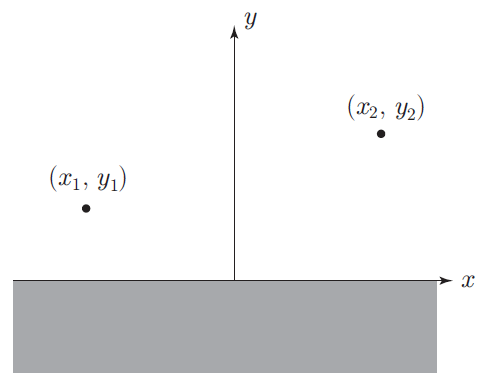
\includegraphics[width=0.6\linewidth]{fig/7.1.png}
	\caption{上半复平面上的CFT中的两点函数。}
\end{figure}
在 $H $内的点上,初级场的定义和复平面上一样。简单起见,考虑共形权为 $(h, h)$ ,自旋为零的初级场$ \phi(z, \bar{z})$ 的两点函数
$$
\left\langle\phi\left(z_{1}, \bar{z}_{1}\right) \phi\left(z_{2}, \bar{z}_{2}\right)\right\rangle
$$
如图7.1。

在Riemann球面上,也就是复平面 $\mathbb{C} $加上无穷远点,全局共形变换是 $PSL(2, \mathbb{C}) $变换
$$
z \rightarrow z^{\prime}=\frac{a z+b}{c z+d}, \quad a d-b c=1, \quad a, b, c, d \in \mathbb{C}
$$
$H $上的全局共形变换必须保持边界的形状,将实轴上的点映到实轴上,因此 $a,b,c,d $必须是实数。这些变换是$ PSL(2, \mathbb{R}) $变换
\begin{equation}
z \rightarrow z^{\prime}=\frac{\alpha z+\beta}{\gamma z+\delta}, \quad \alpha \delta-\beta \gamma=1, \quad \alpha, \beta, \gamma, \delta \in \mathbb{R}
\end{equation}
无穷小变换分为实轴上的平移,标度变换和特殊共形变换
\begin{align} &z \rightarrow z^{\prime}=z+\epsilon_{-1}\\ &z \rightarrow z^{\prime}=z+\epsilon_{0} z\\ &z \rightarrow z^{\prime}=z+\epsilon_{1} z^{2} \end{align}
这里 $\epsilon_{-1}, \epsilon_{0}, \epsilon_{1} $是实数。$ H $上的共形变换受更多限制,因而对称性对关联函数的限制更少。

全局共形变换下,对两点函数有Ward恒等式
\begin{equation}
	\begin{aligned} \left\langle\phi\left(z_{1}, \bar{z}_{1}\right) \phi\left(z_{2}, \bar{z}_{2}\right)\right\rangle=&\left.\left.\prod_{i=1,2}\left(\frac{d z^{\prime}}{d z}\right)^{h}\right|_{z=z_{i}}\left(\frac{d \bar{z}^{\prime}}{d \bar{z}}\right)^{h}\right|_{\bar{z}=\bar{z}_{i}} \\ & \times\left\langle\phi\left(z_{1}^{\prime}, \bar{z}_{1}^{\prime}\right) \phi\left(z_{2}^{\prime}, \bar{z}_{2}^{\prime}\right)\right\rangle \end{aligned} 
\end{equation}
令$ z_{i}=x_{i}+i y_{i} $( $i=1,2$ ),那么两点函数是$ \left(x_{1}, y_{1}, x_{2}, y_{2}\right)$ 的函数。 $x $方向上的平移对称性要求它是 $x_1-x_2 $的函数:
$$
\left\langle\phi\left(z_{1}, \bar{z}_{1}\right) \phi\left(z_{2}, \bar{z}_{2}\right)\right\rangle=G\left(x_{1}-x_{2}, y_{1}, y_{2}\right)
$$
注意,由于存在边界,$ y$ 方向上没有平移对称性。接着,在标度变换
\begin{equation}
	\begin{aligned} &x \rightarrow x^{\prime}=(1+\epsilon) x \\ &y \rightarrow y^{\prime}=(1+\epsilon) y \end{aligned} 
\end{equation}
下,两点函数满足
\begin{equation}
	G\left(x_{1}-x_{2}, y_{1}, y_{2}\right)=(1+\epsilon)^{4 h} G\left(x_{1}^{\prime}-x_{2}^{\prime}, y_{1}^{\prime}, y_{2}^{\prime}\right) 
\end{equation}
记 $u=x_{1}-x_{2}$ ,在$ \epsilon$ 很小时展开得到
\begin{equation}	
4 h G+u \frac{\partial G}{\partial u}+y_{1} \frac{\partial G}{\partial y_{1}}+y_{2} \frac{\partial G}{\partial y_{2}}=0 
\end{equation}
于是 $G$ 可写成
\begin{equation}
	G\left(u, y_{1}, y_{2}\right)=\left(y_{1} y_{2}\right)^{-2 h} \psi\left(\xi_{1}, \xi_{2}\right), \quad \xi_{i}=\frac{y_{i}}{u}
\end{equation} 
最后考虑特殊共形变换 $z^{\prime}=z+\epsilon z^{2} $。$ x,y $坐标变换为:
\begin{equation}
	\begin{aligned} &x \rightarrow x^{\prime}=x+\epsilon\left(x^{2}-y^{2}\right)\\ &y \rightarrow y^{\prime}=y+2 \epsilon x y \end{aligned} 
\end{equation}
Jacobian(之积)是
$$
\frac{d z^{\prime}}{d z} \frac{d \bar{z}^{\prime}}{d \bar{z}}=(1+2 \epsilon z)(1+2 \epsilon \bar{z})=1+4 \epsilon x
$$
因而Ward恒等式给出
\begin{equation}
	G\left(u, y_{1}, y_{2}\right)=\left(1+4 \epsilon x_{1}\right)^{h}\left(1+4 \epsilon x_{2}\right)^{h} G\left(u^{\prime}, y_{1}^{\prime}, y_{2}^{\prime}\right)
\end{equation}
展开得到
\begin{equation}
	\begin{aligned} &\left(x_{1}^{2}-x_{2}^{2}-y_{1}^{2}+y_{2}^{2}\right) \frac{\partial G}{\partial u}+2 x_{1} y_{1} \frac{\partial G}{\partial y_{1}}+2 x_{2} y_{2} \frac{\partial G}{\partial y_{2}} \\ &+4\left(x_{1}+x_{2}\right) h G=0 \end{aligned} 
\end{equation}
与标度变换的方程 (7.9) 联立,得到
\begin{equation}
	\left(y_{2}^{2}-y_{1}^{2}\right) \frac{\partial G}{\partial u}+u\left(y_{1} \frac{\partial G}{\partial y_{1}}-y_{2} \frac{\partial G}{\partial y_{2}}\right)=0 
\end{equation}
代入 (7.10) 给出
\begin{equation}
	\left(\xi_{1}^{2}-\xi_{2}^{2}+1\right) \xi_{1} \frac{\partial \psi}{\partial \xi_{1}}+\left(\xi_{1}^{2}-\xi_{2}^{2}-1\right) \xi_{2} \frac{\partial \psi}{\partial \xi_{2}}=0 
\end{equation}
解得
\begin{equation}
	\psi\left(\xi_{1}, \xi_{2}\right)=\Psi\left(\frac{\left(\xi_{1}+\xi_{2}\right)^{2}+1}{\xi_{1} \xi_{2}}\right) 
\end{equation}
总结一下,$ H$ 上的两点函数形如
\begin{equation}
	\left\langle\phi\left(z_{1}, \bar{z}_{1}\right) \phi\left(z_{2}, \bar{z}_{2}\right)\right\rangle=\left(y_{1} y_{2}\right)^{-2 h} \Psi\left(\frac{\left(x_{1}-x_{2}\right)^{2}+\left(y_{1}+y_{2}\right)^{2}}{y_{1} y_{2}}\right)
\end{equation}
全局共形对称性没有完全确定住它的形式,这同复平面上四点函数的情形一样。事实上,复平面上的点 $\left(z_{1}, z_{2}, \bar{z}_{1}, \bar{z}_{2}\right) $间的交比
\begin{equation}
	\eta=\frac{\left(z_{1}-\bar{z}_{1}\right)\left(z_{2}-\bar{z}_{2}\right)}{\left(z_{1}-\bar{z}_{2}\right)\left(z_{2}-\bar{z}_{1}\right)} 
\end{equation}
是实数,并且是 $PSL(2, \mathbb{R}) $不变量。$ \eta$ 用$ x,y$ 坐标写是
\begin{equation}
	\eta=\frac{4 y_{1} y_{2}}{\left(x_{1}-x_{2}\right)^{2}+\left(y_{1}+y_{2}\right)^{2}} 
\end{equation}
正是 (7.17) 右边括号内参数倒数的4倍。一般地, $H$ 上的$ n$ 点函数可同复平面上的$ 2n$ 点函数对应起来。要看到这一关系,基于无穷小共形Ward恒等式来讨论比较方便。
\section{加倍技巧}
考虑 $H$ 上共形权为$ \left(h_{i}, h_{i}\right)$ ,自旋为零的初级场 $\phi_{i}\left(z_{i}, \bar{z}_{i}\right) $( $i=1, \cdots, n$ )的关联函数
$$
\left\langle\phi_{1}\left(z_{1}, \bar{z}_{1}\right) \cdots \phi_{n}\left(z_{n}, \bar{z}_{n}\right)\right\rangle
$$
$z_i$ 都是$ H$ 内的点。

考虑无穷小共形变换
\begin{equation}
	z \rightarrow z^{\prime}=z+\epsilon(z), \quad \bar{z} \rightarrow \bar{z}^{\prime}=\bar{z}+\bar{\epsilon}(\bar{z})
\end{equation} 
为将边界上的点映到边界上, $\epsilon(z)$ 在实轴上必须要是实的:
\begin{equation}
	\epsilon(z)=\bar{\epsilon}(\bar{z}), \quad z \in \mathbb{R}
\end{equation}
关联函数的Ward恒等式 (3.29) 给出
\begin{equation}
	\begin{aligned} & \int_{C_{+}} d z \frac{1}{2 \pi i} \epsilon(z)\left\langle T(z) \phi_{1} \cdots \phi_{n}\right\rangle-\int_{C_{+}} d \bar{z} \frac{1}{2 \pi i} \bar{\epsilon}(\bar{z})\left\langle\bar{T}(\bar{z}) \phi_{1} \cdots \phi_{n}\right\rangle \\ =&\sum_{i=1}^{n}\left(h_{i} \partial_{i} \epsilon\left(z_{i}\right)+\epsilon\left(z_{i}\right) \partial_{i}+h_{i} \bar{\partial}_{i} \bar{\epsilon}\left(\bar{z}_{i}\right)+\bar{\epsilon}\left(\bar{z}_{i}\right) \bar{\partial}_{i}\right)\left\langle\phi_{1} \cdots \phi_{n}\right\rangle \end{aligned}
\end{equation}
这里,积分路径$ C_+$ 围绕$ H$ 内的$ z_{1}, \cdots, z_{n} $,如图7.2。
\begin{figure}[h]
	\centering
	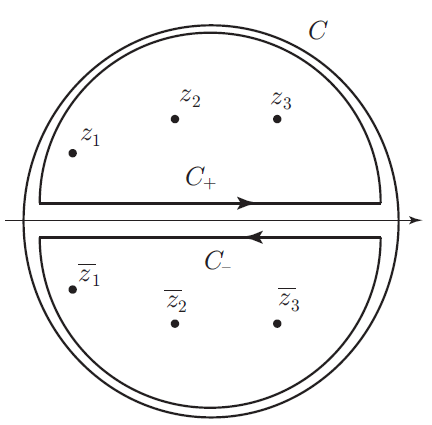
\includegraphics[width=0.6\linewidth]{fig/7.2.png}
	\caption{ $H$上CFT中$n$点函数的Ward恒等式。}
\end{figure}

无穷小共形变换由能动张量 $T_{\mu\nu} $生成。那么,变换不改变边界这一条件,就等价于能量和动量不流经边界。这条件用 $x,y$ 坐标写是 $T_{x y}=0$ ,用复坐标写是
\begin{equation}
	T_{x y}=\frac{1}{4 i}\left(T_{z z}-T_{\bar{z} \bar{z}}\right)=0 
\end{equation}
也就是说,在实轴上有
\begin{equation}
	T(z)=\bar{T}(\bar{z}), \quad z \in \mathbb{R}
\end{equation}
对实轴上取实值的全纯函数 $f(z)$ ,有
\begin{equation}
	f(\bar{z})=\overline{f(z)}
\end{equation} 
这是所谓\textbf{镜像原理}。因为$ \epsilon(z),T(z)$ 在实轴上取实值,它们可根据镜像原理延拓到下半复平面:
\begin{equation}
T(z)=\bar{T}(\bar{z}), \quad \epsilon(z)=\bar{\epsilon}(\bar{z}), \quad \operatorname{Im} z<0
\end{equation} 
因此, (7.22) 左边第二项线积分可改写到下半复平面$ H^{\prime}=\{z \in \mathbb{C}; \operatorname{Im} z<0\} $上:
$$
-\int_{C_{+}} d \bar{z} \frac{1}{2 \pi i} \bar{\epsilon}(\bar{z})\left\langle\bar{T}(\bar{z}) \phi_{1} \cdots \phi_{n}\right\rangle=\int_{C_{-}} d z \frac{1}{2 \pi i}\left\langle T(z) \phi_{1} \cdots \phi_{n}\right\rangle
$$
初级场在$ H'$ 上的位置,是点 $z_i $的复共轭点 $\bar{z}_{i} $,它们关于实轴镜像对称。闭合曲线 $C_- $是 $C_+ $的镜像。在Ward恒等式 (7.22) 中,实轴上的积分相互抵消了,只剩下围绕 $z_{1}, \bar{z}_{1}, \cdots, z_{n}, \bar{z}_{n} $的路径 $C$ 上的积分:
\begin{equation}
	\begin{aligned} & \int_{C} d z \frac{1}{2 \pi i} \epsilon(z)\left\langle T(z) \phi_{1} \cdots \phi_{n}\right\rangle \\ =&\sum_{i=1}^{n}\left(h_{i} \partial_{i} \epsilon\left(z_{i}\right)+\epsilon\left(z_{i}\right) \partial_{i}+h_{i} \partial_{i} \epsilon\left(\bar{z}_{i}\right)+\epsilon\left(\bar{z}_{i}\right) \partial_{i}\right)\left\langle\phi_{1} \cdots \phi_{n}\right\rangle \end{aligned}
\end{equation} 
这给出
\begin{equation}
	\begin{aligned} \left\langle T(z) \phi_{1} \cdots \phi_{n}\right\rangle=& \sum_{i=1}^{n}\left\{\frac{h_{i}}{\left(z-z_{i}\right)^{2}}+\frac{1}{z-z_{i}} \frac{\partial}{\partial z_{i}}+\frac{h_{i}}{\left(z-\bar{z}_{i}\right)^{2}}+\frac{1}{z-\bar{z}_{i}} \frac{\partial}{\partial \bar{z}_{i}}\right\} \\ & \times\left\langle\phi_{1} \cdots \phi_{n}\right\rangle \end{aligned}
\end{equation} 
这说明,上半复平面上 $n$ 点函数的共形Ward恒等式,等价于整个复平面上$ 2n$ 点函数的共形Ward恒等式。这种利用复共轭延拓到下半复平面,在整个复平面上处理的技术称为\textbf{加倍技巧(doubling trick)}。

例如, $H $上的单点函数$ \langle\phi(z, \bar{z})\rangle $等价于复平面上的两点函数$ \langle\phi(z) \phi(\bar{z})\rangle$ :
\begin{equation}
	\langle\phi(z, \bar{z})\rangle=\langle\phi(z) \phi(\bar{z})\rangle=\frac{A}{(2 y)^{2 h}}
\end{equation} \quad \quad (7.29)
$A $是常数。复平面上的单点函数,由共形对称性为零,$ H$ 上的则可非零。类似地, $H$ 上的两点函数$ \left\langle\phi\left(z_{1}, \bar{z}_{1}\right) \phi\left(z_{2}, \bar{z}_{2}\right)\right\rangle $等价于复平面上的四点函数$ \left\langle\phi\left(z_{1}^{\prime}\right) \phi\left(z_{2}^{\prime}\right) \phi\left(z_{3}^{\prime}\right) \phi\left(z_{4}^{\prime}\right)\right\rangle$ ,其中 $z_{1}^{\prime}=z_{1}, z_{2}^{\prime}=z_{2}, z_{3}^{\prime}=\bar{z}_{1} , z_{4}^{\prime}=\bar{z}_{2}$ 。引入交比
\begin{equation}
	\xi=\frac{z_{12}^{\prime} z_{34}^{\prime}}{z_{13}^{\prime} z_{24}^{\prime}}=\frac{\left(z_{1}-z_{2}\right)\left(\bar{z}_{1}-\bar{z}_{2}\right)}{\left(z_{1}-\bar{z}_{1}\right)\left(z_{2}-\bar{z}_{2}\right)}
\end{equation} 
(4.64) 给出
\begin{equation}
	\left\langle\phi\left(z_{1}, \bar{z}_{1}\right) \phi\left(z_{2}, \bar{z}_{2}\right)\right\rangle=\left(\frac{-1}{\left(z_{1}-\bar{z}_{1}\right)^{2}\left(z_{2}-\bar{z}_{2}\right)^{2}}\right)^{h} G_{43}^{21}(\xi)
\end{equation}
其中
\begin{equation}
	G_{43}^{21}(\xi)=\langle\phi(\infty) \phi(1) \phi(\xi) \phi(0)\rangle
\end{equation} 
注意,这里的交比 $\xi $和 (7.18) 定义的交比$ \eta$ 间的关系是
\begin{equation}
	\xi=\frac{\left(x_{1}-x_{2}\right)^{2}+\left(y_{1}-y_{2}\right)^{2}}{-4 y_{1} y_{2}}=\frac{\eta-1}{\eta} 
\end{equation}
此外,如果Virasoro代数有退化表示,可借助零模场得到关于$ G_{43}^{21}(\xi)$ 的解有固定奇点的微分方程,并由此得到关联函数。

例如,我们来计算Ising模型中自旋算符 $\sigma(z, \bar{z}) $的两点函数
$$
\left\langle\sigma\left(z_{1}, \bar{z}_{1}\right) \sigma\left(z_{2}, \bar{z}_{2}\right)\right\rangle
$$
它等价于复平面上的四点函数 (5.137) ,用这里的坐标写是
\begin{equation}
	\begin{aligned} &\left\langle\sigma\left(z_{1}\right) \sigma\left(z_{2}\right) \sigma\left(\bar{z}_{1}\right) \sigma\left(\bar{z}_{2}\right)\right\rangle \\ =&\left(\frac{\left(z_{1}-\bar{z}_{1}\right)\left(z_{2}-\bar{z}_{2}\right)}{\left(z_{1}-z_{2}\right)\left(\bar{z}_{1}-\bar{z}_{2}\right)\left(z_{1}-\bar{z}_{2}\right)\left(z_{2}-\bar{z}_{1}\right)}\right)^{\frac{1}{8}} F(\xi) \end{aligned} 
\end{equation}
共形块 $F(\xi)$ 是超几何微分方程 (5.138) 的解$ \sqrt{1 \pm \sqrt{1-\xi}}$ 的线性组合。于是
\begin{equation}
	\begin{aligned} \left\langle\sigma\left(z_{1}, \bar{z}_{1}\right) \sigma\left(z_{2}, \bar{z}_{2}\right)\right\rangle=&\left(\frac{1}{4 y_{1} y_{2}}\right)^{\frac{1}{8}} \xi^{-\frac{1}{8}}(1-\xi)^{-\frac{1}{8}} \\ & \times\left(a_{+} \sqrt{1+\sqrt{1-\xi}}+a_{-} \sqrt{1-\sqrt{1-\xi}}\right) \end{aligned}
\end{equation} 
$a_\pm $是常数。作为边界条件,我们要求实轴上$ \langle\sigma\rangle=0$ 。固定$ y_1,y_2$ , $\left|x_{1}-x_{2}\right| \rightarrow \infty $时两点函数趋于$ \langle\sigma\rangle\langle\sigma\rangle$ ,从而趋于零。这意味着,右边在 $\xi \rightarrow \infty $时趋于零,由此得到常数应当满足$ a_{+}-ia_{-} =0 $\footnote{J. L. Cardy, Nucl. Phys. B 240 (1984) 514.}。

\section{边界算符}
考虑借助加倍技巧延拓到整个复平面的能动张量 $T(z)$ 。它的模式展开系数定义为\textbf{边界Virasoro算符}
\begin{equation}
	L_{n}=\frac{1}{2 \pi i} \int_{C} d z z^{n+1} T(z) 
\end{equation}
$C $是围绕原点的闭合曲线。不像复平面上的CFT,边界Virasoro算符只有全纯部分。考虑边界Virasoro代数的Hilbert空间。

真空态 $|0\rangle$ 满足
\begin{equation}
	L_{n}|0\rangle=0, \quad(n \geq-1)
\end{equation} 
边界Virasoro算符最高权表示中的最高权态$ |h\rangle $满足
\begin{equation}
	L_{0}|h\rangle=h|h\rangle, \quad L_{n}|h\rangle=0, \quad(n \geq 1)
\end{equation} 
最高权态 $|h\rangle $对应初级场 $\psi(0) $,可由它作用在真空上得到:
\begin{equation}
	|h\rangle=\psi(0)|0\rangle 
\end{equation}
这里的初级场 $\psi(x)$ 是定义在边界(实轴)上的共形场, $x $是实数。定义在边界上的算符称为边界算符。通常定义在上半复平面上的算符$ \phi(z, \bar{z})$ 称为体算符。最高权态 $|h\rangle=\phi(0)|0\rangle $对应的$ L_0$ 的本征值称为边界共形维数。

由全局 $S L(2, \mathbb{R}) $共形对称性,可以确定边界共形维数为 $h_i$ 的边界初级场的关联函数:
\begin{align} &\left\langle\psi_{i}(x) \psi_{j}(y)\right\rangle=\frac{\delta_{i j} A_{i}}{|x-y|^{2 h_{i}}}\\ &\left\langle\psi_{i}\left(x_{1}\right) \psi_{j}\left(x_{2}\right) \psi_{k}\left(x_{3}\right)\right\rangle=\frac{C_{i j k}}{\left|x_{12}\right|^{h_{1}+h_{2}-h_{3}}\left|x_{23}\right|^{h_{2}+h_{3}-h_{1}}\left|x_{31}\right|^{h_{1}+h_{3}-h_{2}}} \end{align}
其中$ x_{i j}=x_{i}-x_{j}$ 。
\begin{figure}[h]
	\centering
	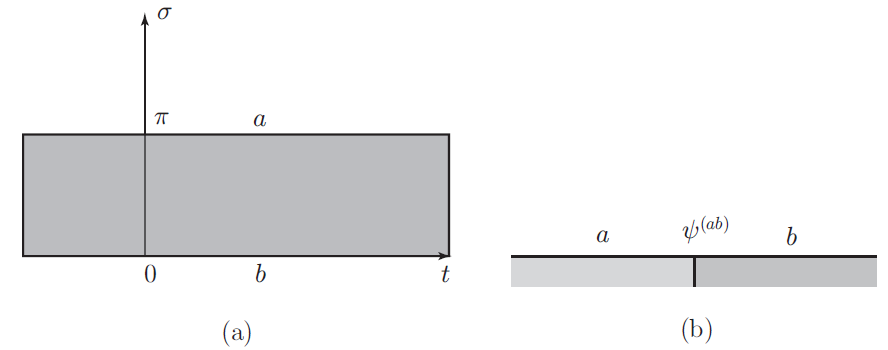
\includegraphics[width=0.6\linewidth]{fig/7.3.png}
	\caption{(a)带和边界条件。(b)连接边界条件$a$和$b$的边界算符$\psi^{(ab)}$。}
\end{figure}

在实轴上插入边界初级场会发生什么?我们用共形变换
\begin{equation}
	w=\log z=t+i \sigma
\end{equation} 
将上半复平面映成宽 $\pi $的无穷长带,如图7.3(a)。Hamiltonian是时间$ t $方向上的演化算符
\begin{equation}
	H=\int_{0}^{\pi} T_{t t} d \sigma-\frac{c}{24}
\end{equation}
6.1节讨论过,常数项来自Schwarz导数。借助加倍技巧,Hamiltonian可用边界Virasoro算符写成
\begin{equation}
	H=L_{0}-\frac{c}{24}
\end{equation} 
变换不改变边界这一条件,等价于 $T(z)=\bar{T}(\bar{z})$ ( $z\in\mathbb{R}$ ),用$ t,\sigma $坐标写是 $T_{t \sigma}=0$ ( $\sigma=0,\pi$ )。

边界条件有很多种。上下两边界上可以施加不同条件,确保仍然满足变换不改变边界这一条件即可。带上端(对应负半实轴)的边界条件记作$ a$ ,下端(对应正实半轴)的则记作 $b$ ,整个边界条件记作$ (ab)$ 。边界条件不同,意味着原点处不连续。在BCFT中,边界条件的变化可通过在$ z=0 $( $t=-\infty $)处插入边界初级场实现。对应边界条件$ (ab)$ 的边界初级场记作$ \psi^{(a b)}(x)$ ,如图7.3(b)。这种造成插入点左右边界条件不同的算符,有时称为边界改变算符。注意,恒等算符 $\boldsymbol{I}(x) $不会改变边界条件。\footnote{边界条件不同,也就破坏了原点处的平移对称性,这在径向量子化中意味着 $z=0 $处的“真空态”不再被$ L_{-1}$ 湮灭。根据态-算符对应,自然就相当于在 $z=0 $处插入算符。}

带边界条件 $(ab) $的系统的Hamiltonian记作 $H_{a b} $。$ H_{ab} $的本征空间可分解成边界Virasoro代数的不可约表示之和。最高权表示$ [h]$ 在分解中出现的次数记作 $n_{a b}^{h}$ 。满足$ n_{a b}^{h} \neq 0 $的最小的$ h $记作 $h_{ab}$ 。相应的边界初级场 $\psi^{(a b)}(x) $是基本的边界改变算符,$ h_{ab}$ 是它的边界共形维数。边界共形维数更高的场,可通过令其它算符作用在这个态上得到。特别地,在两侧边界条件相同的情形( a=b ),这个态是真空态 $|0\rangle$ ,对应恒等算符 $\boldsymbol{I}(x) $。 $h_{ab}=0$ , $[h_{ab}] $在分解中出现$ n_{a a}^{0}=1$ 次。\footnote{原书接下来的一句论证,我(\href{https://www.zhihu.com/people/wo-bei-56}{@笠道梓})不认同,发现文献中也有争议,因此按个人更认同的观点进行了改写。}

插入多个场时,我们只考虑最左侧和最右侧边界条件相同的情形,这相当于不在 $x=\pm \infty $处插入场,关联函数中就要出现额外的Kronecker delta符号。边界共形维数为 $h_i $的边界改变初级场 $\psi_{i}^{(a b)}(x)$ 的两点和三点函数是
\begin{align} &\left\langle\psi_{i}^{(a b)}(x) \psi_{j}^{(b c)}(y)\right\rangle=\frac{\delta_{i j} \delta_{a c} A_{i}^{a b}}{|x-y|^{2 h_{i}}}\\ &\left\langle\psi_{i}^{(a b)}\left(x_{1}\right) \psi_{j}^{(b c)}\left(x_{2}\right) \psi_{k}^{(c d)}\left(x_{3}\right)\right\rangle=\frac{\delta_{a d} C_{i j k}^{a b c}}{\left|x_{12}\right|^{h_{1}+h_{2}-h_{3}}\left|x_{23}\right|^{h_{2}+h_{3}-h_{1}}\left|x_{31}\right|^{h_{1}+h_{3}-h_{2}}} \end{align}

为确定这些三点函数中的系数,我们必须知道初级场OPE的结构。BCFT中的初级场包括体初级场$ \phi_{i}(z, \bar{z}) $和边界初级$场 \psi_{i}^{(a b)}(x)$ ,它们间的OPE都要纳入考虑。体初级场自身间的OPE和复平面上的形式相同,边界初级场自身间的OPE与上述两点和三点函数的结构一致。此外,体初级场靠近实轴时,同它的镜像生成了新的OPE。在BCFT中, $\phi_{i}(z, \bar{z})$ 的体共形权为 $\left(h_{i}, h_{i}\right)$ 时,OPE是(考虑自旋为零的场)\footnote{J. L. Cardy and D. C. Lewellen, Phys. Lett. B 259 (1991) 274.}\footnote{R. E. Behrend, P. A. Pearce, V. B. Petkova and J. B. Zuber, Nucl. Phys. B 570 (2000) 525 [arXiv:hep-th/9908036].}\footnote{I. Runkel, Nucl. Phys. B 549 (1999) 563 [arXiv:hep-th/9811178].}
\begin{align} &\phi_{i}(z, \bar{z}) \phi_{j}(w, \bar{w})=\sum_{k}|z-w|^{2\left(h_{k}-h_{i}-h_{j}\right)} C_{i j}^{k} \phi_{k}(w, \bar{w})\\ &\phi_{i}(z, \bar{z})=\sum_{k}{ }^{(a)} B_{i}^{k} \psi_{k}^{(a a)}(x)(2 y)^{h_{k}-2 h_{i}} \\ &\psi_{i}^{(a b)}(x) \psi_{j}^{(b c)}(y)=\sum_{k}(x-y)^{h_{k}-h_{i}-h_{j}} C_{i j}^{(a b c) k} \psi_{k}^{(a c)}(y) \end{align}
系数$ C_{i j}^{k}, {}^{(a)} B_{i}^{k}, C_{i j}^{(a b c) k}$ 表征着BCFT中的OPE。

\section{边界态}
在无穷长带的时间 $t $方向加上周期性:
$$
t \equiv t+2 \pi \delta
$$
就得到圆环,如图7.4。
\begin{figure}[h]
	\centering
	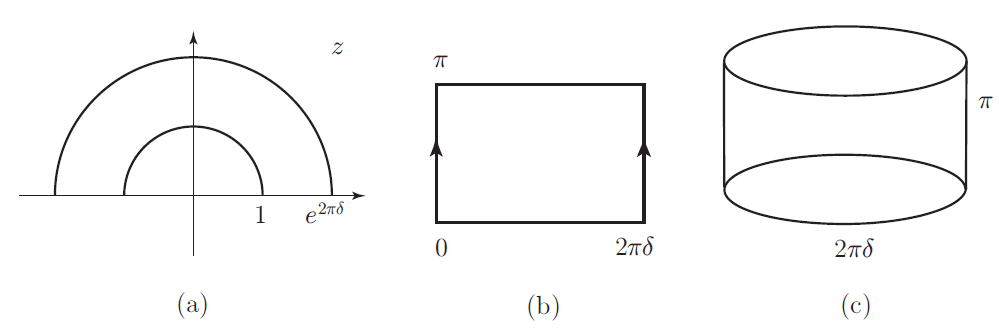
\includegraphics[width=0.6\linewidth]{fig/7.4.png}
	\caption{(a)$z$平面上的圆环,(b)长$2\pi \delta$,宽$\pi$的矩形,左右两边粘起来就得到圆环,(c)圆环。}
\end{figure}

这是一个带两条边界的曲面,如果再将这两条边界粘起来,就得到环面。

各边界条件记作$ a,b $,相应的Hamiltonian记作 $H_{ab} $,圆环上的配分函数是
\begin{equation}
	Z_{a b}(\delta)=\operatorname{Tr} e^{-2 \pi \delta H_{a b}} 
\end{equation}
因为Hamiltonian可用边界Virasoro算符写成 $H_{a b}=L_{0}-\frac{c}{24} $,它的本征空间可分解成边界Virasoro代数的最高权表示之和,我们有
\begin{equation}
	Z_{a b}(\delta)=\operatorname{Tr} q^{L_{0}-\frac{c}{24}}=\sum_{i} n_{a b}^{i} \chi_{h_{i}}(q)
\end{equation} 
这里$ q=e^{-2 \pi \delta} $。这对应将环面的模参数取成纯虚数 $\tau=i \delta $。$ \chi_{h_{i}}(q)=q^{-\frac{c}{24}} \operatorname{Tr}_{\left[h_{i}\right]} q^{L_{0}} $是边界Virasoro代数最高权表示$ [h_i]$ 的特征标, $n_{a b}^{i} $是$ [h_i] $在分解中出现的次数。

在环面的情形,配分函数模不变。特别地,将 $\tau $映成$ -1/\tau $的 $S $变换,交换了环面的时间和空间方向。在圆环的情形,模不变性对配分函数施加了什么限制呢?在 $S $变换下,
$$
q=e^{2 \pi i \tau} \rightarrow \tilde{q}=e^{-\frac{2 \pi i}{\tau}}=e^{-\frac{2 \pi}{\delta}}
$$
特征标的变换行为给出
\begin{equation}
	\chi_{h_{i}}(q)=\sum_{j} S_{i}^{j} \chi_{h_{j}}(\tilde{q})
\end{equation} 
于是配分函数是
\begin{equation}
	Z_{ab}=\sum_{i, j} n_{a b}^{i} S_{i}^{j} \chi_{h_{j}}(\tilde{q})
\end{equation} \quad \quad (7.53)
\begin{figure}[h]
	\centering
	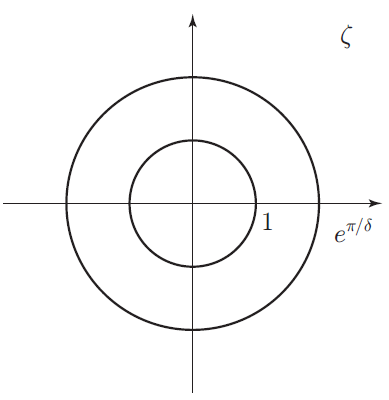
\includegraphics[width=0.6\linewidth]{fig/7.5.png}
	\caption{$\zeta$平面上的圆环。}
\end{figure}

另一方面,在圆环的情形,时间坐标 $t $和空间坐标 $\sigma $交换,周向成了空间方向,柱向则成了时间方向。变换后的Hamiltonian $H^{P} $是柱向的演化算符,我们用它来重写配分函数。共形变换
\begin{equation}
	\zeta=e^{-\frac{i}{\delta} w}=e^{-\frac{i}{\delta}(t+i \sigma)} 
\end{equation}\quad \quad (7.54)
下,图7.4(b)中的矩形映成图7.5中$ \zeta $平面上的圆环。为同之前的边界Virasoro算符区分,我们将$ \zeta$ 平面上的体Virasoro算符记作 $\hat{L}_{n}, \bar{\hat{L}}_{n}$ 。$ H^P $可用它们写成
\begin{equation}
	H^{P}=\hat{L}_{0}+\bar{\hat{L}}_{0}-\frac{c}{12}
\end{equation}
$\zeta$ 平面上的配分函数是从$ |\zeta|=1 $时的态$|a\rangle $到 $|\zeta|=e^{\frac{\pi}{\delta}} $时的态 $|b\rangle $的跃迁矩阵元
\begin{equation}
	Z_{ab}= \langle b |e^{-\frac{\pi}{\delta} H^{P}} | a \rangle= \langle b |\tilde{q}^{\frac{1}{2}\left(\hat{L}_{0}+\bar{\hat{L}}_{0}-\frac{c}{12}\right)} | a \rangle
\end{equation}
态 $|a\rangle,|b\rangle$ 称为\textbf{边界态},它们是Virasoro算符 $\hat{L}_{n}$, $\bar{\hat{L}}_{n}$ 作用的空间中的元素。

我们来进一步考察边界态的性质。能动张量可模式展开成
\begin{align} &\hat{T}(\zeta)=\sum_{n=-\infty}^{\infty} \hat{L}_{n} \zeta^{-n-2}\\ &\bar{\hat{T}}(\bar{\zeta})=\sum_{n=-\infty}^{\infty} \bar{\hat{L}}_{n} \bar{\zeta}^{-n-2} \end{align}
边界上\footnote{ z 平面上变换不改变边界的条件 (7.24) ,结合能动张量的变换行为 (3.52) 得到}$ \zeta^2\hat{T}(\zeta)-\bar{\zeta}^2\bar{\hat{T}}(\bar{\zeta})=0$ ,在边界 $|\zeta|=1 $上用相应的边界态 $|B\rangle $写是
\begin{equation}
	\left.(\zeta^2\hat{T}(\zeta)-\bar{\zeta}^2\bar{\hat{T}}(\bar{\zeta}))\right|_{|\zeta|=1}|B\rangle=0 
\end{equation}
用Virasoro算符写是
\begin{equation}
	\left(\hat{L}_{n}-\bar{\hat{L}}_{-n}\right)|B\rangle=0
\end{equation}

我们来在张量积空间 $[h] \otimes[\bar{h}]$ 中构造满足 (7.59) 的边界态 $|B\rangle $, $[h] $是$ \hat{L}_{n} $的最高权表示, $[\bar{h}] $是 $\bar{\hat{L}}_{n} $的最高权表示。注意,$ n=0$ 时,这个条件是
$$
\hat{L}_{0}|B\rangle=\bar{\hat{L}}_{0}|B\rangle
$$
这给出 $h=\bar{h}$ 。考虑$ [h]$ 级为 $N$ 的子空间,它的维数记作$d_{h}(N) $,标准正交基记作
$$
|h, N ; j\rangle, \quad j=1, \cdots, d_{h}(N)
$$
类似地,考虑 $[\bar{h}] $级为 $N $的子空间,标准正交基记作 $\overline{|h, N ; j\rangle} $。张量积空间的基从而是 $|h, N ; j\rangle\otimes\overline{|h, N ; j\rangle} $。引入满足
\begin{align} &U \overline{|h, 0\rangle}=\overline{|h, 0\rangle}^{*} \\ &U \bar{\hat{L}}_{n}=\bar{\hat{L}}_{n} U \end{align}
的反酉算符 $U $\footnote{反酉给出 $\langle Ux|Uy\rangle=\langle y|x\rangle$ },定义态
\begin{equation}
	|h\rangle\rangle=\sum_{N=0}^{\infty} \sum_{j=1}^{d_{h}(N)}|h, N ; j\rangle \otimes U \overline{|h, N ; j\rangle}
\end{equation}
这称为\textbf{Ishibashi态}\footnote{N. Ishibashi, Mod. Phys. Lett. A 4 (1989) 251.}。Ishibashi态是 $[h] \otimes[\bar{h}] $中 (7.59) 的唯一解。取 $\left(\hat{L}_{n}-\bar{\hat{L}}_{-n}\right)|h\rangle \rangle$ 和一般态 $\left\langle h, N_{1} ; k\right| \otimes U \overline{\left\langle h, N_{2} ; l\right|} $的内积,由基的标准正交性和算符的反酉性得到\footnote{由于$ h=\bar{h}$ ,相应表示中的矩阵元可以互相代换,我们有 $\langle x|A|y\rangle=\langle \bar{x}|\bar{A}|\bar{y}\rangle $。}
\begin{equation}
	\begin{aligned} & \left(\left\langle h, N_{1} ; k\right| \otimes U \overline{\left\langle h, N_{2} ; l\right|}\right)\left(\hat{L}_{n}-\bar{\hat{L}}_{-n}\right)|h\rangle \rangle \\ =& \sum_{N} \sum_{j}\left( \langle h, N_{1} ; k |\hat{L}_{n} | h, N ; j \rangle U \overline{\left\langle h, N_{2} ; l\right|} U \overline{|h, N ; j\rangle}\right.\\&\left.-\left\langle h, N_{1} ; k | h, N ; j\right\rangle U \overline{\left\langle h, N_{2} ; l\right|} \bar{\hat{L}}_{-n} U \overline{|h, N ; j\rangle}\right) \\ =& \langle h, N_{1} ; k |\hat{L}_{n} | h, N_{2} ; l \rangle- \langle h, N_{1} ;k |\hat{L}_{-n}^\dagger | h, N_{2} ; l \rangle \\ =& 0 \end{aligned}
\end{equation}
最后一个等号用了Hermite性$ \hat{L}_{-n}^{\dagger}=\hat{L}_{n}$ 。

Ishibashi态间的矩阵元可以算出是
\begin{equation}
	\begin{aligned} \langle \langle h^{\prime} |\tilde{q}^{\frac{1}{2}\left(\hat{L}_{0}+\bar{\hat{L}}_{0}-\frac{c}{12}\right)} | h \rangle \rangle=& \sum_{N^{\prime}=0}^{\infty} \sum_{j^{\prime}=1}^{d_{h^{\prime}}\left(N^{\prime}\right)} \sum_{N=0}^{\infty} \sum_{j=1}^{d_{h}(N)}\left\langle h^{\prime}, N^{\prime} ; j^{\prime}\right| \otimes U \bar{\left\langle h^{\prime}, N^{\prime} ; j^{\prime}\right|} \\ & \times \tilde{q}^{\frac{1}{2}\left(\hat{L}_{0}+\bar{\hat{L}}_{0}-\frac{c}{12}\right)}|h, N ; j\rangle \otimes U \overline{|h, N ; j\rangle} \\ =& \delta_{h^{\prime}, h} \sum_{N=0}^{\infty} \sum_{j=1}^{d_{h}(N)} \tilde{q}^{h+N-\frac{c}{24}} \\ =& \delta_{h^{\prime}, h} \sum_{N=0}^{\infty} d_{h}(N) \tilde{q}^{h+N-\frac{c}{24}} \\ =& \delta_{h, h^{\prime}} \chi_{h}(\tilde{q}) \end{aligned}
\end{equation} 
$\chi_{h}(\tilde{q}) $是Virasoro代数的特征标。

边界态 $|a\rangle $可用Ishibashi态展开成
\begin{equation}
	|a\rangle=\sum_{h}|h\rangle \rangle\langle\langle h |a\rangle
\end{equation}
代入配分函数 (7.56) 得到
\begin{equation}
	Z_{ab}=\sum_{h}\langle b | h\rangle \rangle \langle\langle h |a\rangle \chi_{h}(\tilde{q})
\end{equation} 
与 (7.53) 比对,我们得到矩阵元$ \langle\langle h |a\rangle $要满足
\begin{equation}
	\sum_{i} n_{b a}^{i} S_{i}^{j}=\left\langle b | h_{j} \rangle\right\rangle\left\langle\left\langle h_{j} |a\right\rangle\right.
\end{equation}
这称为\textbf{Cardy条件},满足这条件的边界态 $|a\rangle$ 称为\textbf{Cardy态}。

Virasoro代数最高权表示$ [h_j] $对应的边界条件记作 $\tilde{j}$ ,我们来构造边界态$ |\tilde{j}\rangle$ 。首先,恒等表示(记作$ j=0$ )对应的边界态记作 $|\tilde{0}\rangle$ 。这对应边界条件 $(\tilde{0}\tilde{0})$ ,Hamiltonian$ H_{\tilde{0} \tilde{0}}$ 的本征空间分解中只有恒等表示, $n_{\tilde{0} \tilde{0}}^{i}=\delta_{0}^{i} $,代入Cardy条件得到
\begin{equation}
	S_{0}^{j}= | \langle\tilde{0} |h_{j} \rangle \rangle |^{2}
\end{equation} 
这可写成
\begin{equation}
	|\tilde{0}\rangle=\sum_{j}\left(S_{0}^{j}\right)^{\frac{1}{2}} |h_{j} \rangle \rangle
\end{equation}
类似地,边界条件 $(\tilde{0}\tilde{l})$ ,对应Hamiltonian $H_{\tilde{0} \tilde{l}}$ 的本征空间分解中只有表示 $[h_l] $,对应边界态 $|\tilde{l}\rangle$ 。这时 $n_{\tilde{0} \tilde{l}}^{i}=\delta_{l}^{i}$ ,Cardy条件是
\begin{equation}
	S_l^j=\langle \tilde{0}|h_j\rangle\rangle\langle\langle h_j|l\rangle
\end{equation}
即
\begin{equation}
	\langle \langle h_{j} | \tilde{l} \rangle=\frac{S_{l}^{j}}{\left(S_{0}^{j}\right)^{1 / 2}} 
\end{equation}
于是
\begin{equation}
	|\tilde{l}\rangle=\sum_{j} \frac{S_{l}^{j}}{\left(S_{0}^{j}\right)^{1 / 2}}\left|h_{j}\right\rangle \rangle
\end{equation}
此外,取 $n_{\tilde{l} \tilde{0}}^{i}=\delta_{l}^{i}$ 给出左矢
\begin{equation}
	\langle\tilde{l}|=\sum_{j} \frac{\left(S_{l}^{j}\right)^{*}}{\left(S_{0}^{j}\right)^{1 / 2}}\left\langle\left\langle h_{j}\right|\right. 
\end{equation}
为方便,再定义
\begin{equation}
	\langle\tilde{l}^{\vee} |=\sum_{j} \frac{S_{l}^{j}}{\left(S_{0}^{j}\right)^{1 / 2}} \langle\left\langle h_{j}\right| 
\end{equation}
在极小模型的情形,模$ S $矩阵实对称,不必区分它们。

以Ising模型为例。由模 $S$ 矩阵 (6.139) , $h=0,1/2,1/16$ 初级态对应的Ishibashi态记作 $|0\rangle\rangle,|\epsilon\rangle\rangle,|\sigma\rangle\rangle$ ,那么Cardy态是
\begin{equation}
	\begin{aligned} & |\tilde{0}\rangle=\frac{1}{\sqrt{2}}|0\rangle \rangle+\frac{1}{\sqrt{2}}|\epsilon\rangle \rangle+\frac{1}{2^{\frac{1}{4}}}|\sigma\rangle \rangle \\ & \left|\frac{\tilde{1}}{2}\right\rangle=\frac{1}{\sqrt{2}}|0\rangle \rangle+\frac{1}{\sqrt{2}}|\epsilon\rangle \rangle-\frac{1}{2^{\frac{1}{4}}}|\sigma\rangle \rangle \\ & \left|\frac{\tilde{1}}{16}\right\rangle=|0\rangle \rangle-|\epsilon\rangle \rangle \end{aligned}
\end{equation}
用Ising模型的语言来说, $|\tilde{0}\rangle $是自旋向上的边界态, $\left|\frac{\tilde{1}}{2}\right\rangle$ 是自旋向下的边界态, $\left|\frac{\tilde{1}}{16}\right\rangle $是自由边界条件,由此我们记
\begin{equation}
	\begin{aligned} &|+\rangle=|\tilde{0}\rangle \\ &|-\rangle=\left|\frac{\tilde{1}}{2}\right\rangle \\ &|f\rangle=\left|\frac{\tilde{1}}{16}\right\rangle \end{aligned} 
\end{equation}
各边界条件下的配分函数是
\begin{align} &Z_{++}=Z_{--}=\frac{1}{2} \chi_{0}+\frac{1}{2} \chi_{\frac{1}{2}}+\frac{1}{\sqrt{2}} \chi_{\frac{1}{16}} \\ &Z_{f f}=\chi_{0}+\chi_{\frac{1}{2}}\\ &Z_{+-}=\frac{1}{2} \chi_{0}+\frac{1}{2} \chi_{\frac{1}{2}}-\frac{1}{\sqrt{2}} \chi_{\frac{1}{16}}\\ &Z_{+f}=Z_{-f}=\frac{1}{\sqrt{2}} \chi_{0}-\frac{1}{\sqrt{2}} \chi_{\frac{1}{2}} \end{align}

\subsection{BCFT和Verlinde公式}
Cardy态的表达式代入Cardy条件得到
\begin{equation}
	\sum_{i} S_{i}^{j} n_{\tilde{k}^{\vee} \tilde{l}}^{i}=\frac{S_{k}^{j} S_{l}^{j}}{S_{0}^{j}}
\end{equation} 
如果这里的 $n_{\tilde{k}^{\vee} \tilde{l}}^{i} $等于融合系数 $N_{k l}^{i}$ ,那么这个式子就是Verlinde公式 (6.167) 。
\begin{figure}[h]
	\centering
	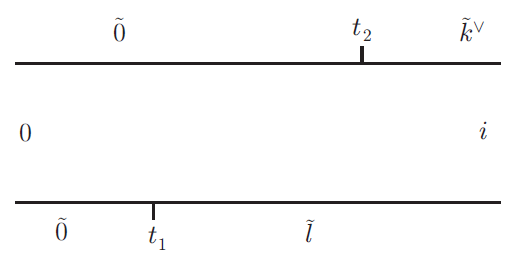
\includegraphics[width=0.6\linewidth]{fig/7.6.png}
	\caption{带上的BCFT和Verlinde公式。}
\end{figure}

Cardy从BCFT的角度给出了Verlinde公式的解释\footnote{J. L. Cardy, Nucl. Phys. B 324 (1989) 581.}。考虑带上的BCFT,假定某些时刻边界条件发生了改变,如图7.6。 $t<t_1 $时边界条件是 $(\tilde{0}\tilde{0})$ 。 $t=t_1$ 时下端的边界条件从 $\tilde{0}$ 变为 $\tilde{l}$ ,这相当于插入边界算符 $\psi_{\tilde{l} \tilde{0}} $。那么Hamiltonian从 $H_{\tilde{0} \tilde{0}} $变为$ H_{\tilde{l} \tilde{0}} $,$ n_{b a}^{i}$ 从 $n_{\tilde{0} \tilde{0}}^{i}=\delta_{0}^{i}$ 变为 $n_{\tilde{0} \tilde{l}}^{i}=\delta_{l}^{i} $,这相当于融合系数从 $N_{00}^{i}=\delta_{0}^{i} $变为 $N_{l 0}^{i}=\delta_{l}^{i}$ 。 $t=t_2>t_1$ 时上端的边界条件从 $\tilde{0} $变为 $\tilde{k}^{\vee} $,这相当于插入边界算符 $\psi_{\tilde{k} ^\vee \tilde{0}}$ ,那么 $n_{b a}^{i}$ 从 $n_{\tilde{l}\tilde{0}}^{i} $变为$ n_{\tilde{k}^{\vee} \tilde{l}}^{i} $。这个数等于表示 $k^{\vee} $对应的场和表示$ l$ 对应的场组合起来再分解时,表示$ i $对应的场出现的次数,就是融合系数 $N_{k l}^{i}$ 。





\backmatter
% bibliography, glossary and index would go here.

\end{document}